\documentclass[twoside]{book}

% Packages required by doxygen
\usepackage{fixltx2e}
\usepackage{calc}
\usepackage{doxygen}
\usepackage[export]{adjustbox} % also loads graphicx
\usepackage{graphicx}
\usepackage[utf8]{inputenc}
\usepackage{makeidx}
\usepackage{multicol}
\usepackage{multirow}
\PassOptionsToPackage{warn}{textcomp}
\usepackage{textcomp}
\usepackage[nointegrals]{wasysym}
\usepackage[table]{xcolor}

% Font selection
\usepackage[T1]{fontenc}
\usepackage[scaled=.90]{helvet}
\usepackage{courier}
\usepackage{amssymb}
\usepackage{sectsty}
\renewcommand{\familydefault}{\sfdefault}
\allsectionsfont{%
  \fontseries{bc}\selectfont%
  \color{darkgray}%
}
\renewcommand{\DoxyLabelFont}{%
  \fontseries{bc}\selectfont%
  \color{darkgray}%
}
\newcommand{\+}{\discretionary{\mbox{\scriptsize$\hookleftarrow$}}{}{}}

% Page & text layout
\usepackage{geometry}
\geometry{%
  a4paper,%
  top=2.5cm,%
  bottom=2.5cm,%
  left=2.5cm,%
  right=2.5cm%
}
\tolerance=750
\hfuzz=15pt
\hbadness=750
\setlength{\emergencystretch}{15pt}
\setlength{\parindent}{0cm}
\setlength{\parskip}{3ex plus 2ex minus 2ex}
\makeatletter
\renewcommand{\paragraph}{%
  \@startsection{paragraph}{4}{0ex}{-1.0ex}{1.0ex}{%
    \normalfont\normalsize\bfseries\SS@parafont%
  }%
}
\renewcommand{\subparagraph}{%
  \@startsection{subparagraph}{5}{0ex}{-1.0ex}{1.0ex}{%
    \normalfont\normalsize\bfseries\SS@subparafont%
  }%
}
\makeatother

% Headers & footers
\usepackage{fancyhdr}
\pagestyle{fancyplain}
\fancyhead[LE]{\fancyplain{}{\bfseries\thepage}}
\fancyhead[CE]{\fancyplain{}{}}
\fancyhead[RE]{\fancyplain{}{\bfseries\leftmark}}
\fancyhead[LO]{\fancyplain{}{\bfseries\rightmark}}
\fancyhead[CO]{\fancyplain{}{}}
\fancyhead[RO]{\fancyplain{}{\bfseries\thepage}}
\fancyfoot[LE]{\fancyplain{}{}}
\fancyfoot[CE]{\fancyplain{}{}}
\fancyfoot[RE]{\fancyplain{}{\bfseries\scriptsize Generated by Doxygen }}
\fancyfoot[LO]{\fancyplain{}{\bfseries\scriptsize Generated by Doxygen }}
\fancyfoot[CO]{\fancyplain{}{}}
\fancyfoot[RO]{\fancyplain{}{}}
\renewcommand{\footrulewidth}{0.4pt}
\renewcommand{\chaptermark}[1]{%
  \markboth{#1}{}%
}
\renewcommand{\sectionmark}[1]{%
  \markright{\thesection\ #1}%
}

% Indices & bibliography
\usepackage{natbib}
\usepackage[titles]{tocloft}
\setcounter{tocdepth}{3}
\setcounter{secnumdepth}{5}
\makeindex

% Hyperlinks (required, but should be loaded last)
\usepackage{ifpdf}
\ifpdf
  \usepackage[pdftex,pagebackref=true]{hyperref}
\else
  \usepackage[ps2pdf,pagebackref=true]{hyperref}
\fi
\hypersetup{%
  colorlinks=true,%
  linkcolor=blue,%
  citecolor=blue,%
  unicode%
}

% Custom commands
\newcommand{\clearemptydoublepage}{%
  \newpage{\pagestyle{empty}\cleardoublepage}%
}

\usepackage{caption}
\captionsetup{labelsep=space,justification=centering,font={bf},singlelinecheck=off,skip=4pt,position=top}

%===== C O N T E N T S =====

\begin{document}

% Titlepage & ToC
\hypersetup{pageanchor=false,
             bookmarksnumbered=true,
             pdfencoding=unicode
            }
\pagenumbering{alph}
\begin{titlepage}
\vspace*{7cm}
\begin{center}%
{\Large T\+D\+J\+A\+N\+G\+OH \\[1ex]\large 1.\+1 }\\
\vspace*{1cm}
{\large Generated by Doxygen 1.8.13}\\
\end{center}
\end{titlepage}
\clearemptydoublepage
\pagenumbering{roman}
\tableofcontents
\clearemptydoublepage
\pagenumbering{arabic}
\hypersetup{pageanchor=true}

%--- Begin generated contents ---
\chapter{T\+D\+J\+A\+N\+G\+OH Doxyfile documentation}
\label{index}\hypertarget{index}{}Welcome to the doxygen documentation of the T\+D\+J\+A\+N\+G\+OH interface.

You can find several informations about the T\+D\+J\+A\+N\+G\+OH class and the D\+J\+A\+N\+G\+OH generator.

For more informations about running the package, look at the \hyperlink{md__r_e_a_d_m_e}{R\+E\+A\+D\+ME}.

For any problem, input, questions \+: \href{mailto:nicolas.pierre@cern.ch}{\tt nicolas.\+pierre@cern.\+ch} 
\chapter{T\+D\+J\+A\+N\+G\+OH Usage Instructions}
\label{md__r_e_a_d_m_e}
\Hypertarget{md__r_e_a_d_m_e}
\subsection*{Requirements}

G\+CC $>$ 4.\+4.\+7 with build-\/in G\+F\+O\+R\+T\+R\+AN

R\+O\+OT $>$ 5.\+34/32

L\+H\+A\+P\+DF 5.\+9.\+1 (in any case lower than L\+H\+A\+P\+DF 6.\+x.\+x) \href{https://www.hepforge.org/downloads/lhapdf}{\tt Download L\+H\+A\+P\+DF 5.\+x.\+x}

C\+E\+R\+N\+L\+IB (2006) \href{http://cernlib.web.cern.ch/cernlib/version.html}{\tt Download C\+E\+R\+N\+L\+IB}

(Tested on L\+X\+P\+L\+US and C\+C\+A\+GE)

\subsection*{Environment variables}

After recovering the package, export the following variables (better in .bashrc or similar) \+:

{\ttfamily export T\+D\+J\+A\+N\+G\+OH=/path/to/\+T\+D\+J\+A\+N\+G\+O\+H/} {\ttfamily export L\+H\+A\+P\+D\+F5=/path/to/\+L\+H\+A\+P\+D\+F5/}

\subsection*{Setup \& Build}

To setup \+: {\ttfamily make setup}

To build \+: {\ttfamily make}

\subsection*{Test Programs}

See more on \hyperlink{md_test__t_e_s_t_p_r_o_g_r_a_m_s}{test programs}..

\subsection*{Utilities Programs}

See more on \hyperlink{md_utils__u_t_i_l_s_p_r_o_g_r_a_m_s}{utilities programs}..

\subsection*{More informations on Djangoh}

The \href{http://wwwthep.physik.uni-mainz.de/~hspiesb/djangoh/djangoh_m.4.6.6.ps.gz}{\tt D\+J\+A\+N\+G\+OH manual Version 1.\+6} contains the description of input options and includes short lists of most important changes with respect to previous versions. The T\+D\+J\+A\+N\+G\+OH manual is coming soon !

\subsection*{Contact}

For any problem, input, questions \+: \href{mailto:nicolas.pierre@cern.ch}{\tt nicolas.\+pierre@cern.\+ch} 
\chapter{Test programs}
\label{md_test__t_e_s_t_p_r_o_g_r_a_m_s}
\Hypertarget{md_test__t_e_s_t_p_r_o_g_r_a_m_s}
You can find two different programs \+:
\begin{DoxyItemize}
\item One is {\ttfamily test} and is used to test the generator. The usage is the following \+:
\begin{DoxyItemize}
\item {\ttfamily ./test \mbox{[}inputfile\mbox{]} \mbox{[}nb\+\_\+evts\mbox{]} + flags}
\item The input file is a specified .xml config file. You can find a template in {\ttfamily utils/}
\item Flags can be \+:
\begin{DoxyItemize}
\item {\ttfamily -\/energy \mbox{[}e\mbox{]}} \+: nominal energy of the beam.
\item {\ttfamily -\/verbose \mbox{[}v\mbox{]}} \+: v=0/1/2, default is 1. Use 0 when in batch mode.
\item {\ttfamily -\/rand \mbox{[}r\mbox{]}} \+: r=0/1, gaussian randomization of input energy within ±40 GeV relative to nominal energy.
\item {\ttfamily -\/finalstate} \+: save the final states inside a file (eg. for semi-\/inclusive correction calculation)
\end{DoxyItemize}
\end{DoxyItemize}
\item The other is {\ttfamily xsgen} and is used for inclusive cross-\/section generation. The usage is the following \+:
\begin{DoxyItemize}
\item {\ttfamily ./xsgen \mbox{[}inputfile\mbox{]} \mbox{[}R\+C(1)/\+Born(0)\mbox{]}} 
\end{DoxyItemize}
\end{DoxyItemize}
\chapter{Utils programs}
\label{md_utils__u_t_i_l_s_p_r_o_g_r_a_m_s}
\Hypertarget{md_utils__u_t_i_l_s_p_r_o_g_r_a_m_s}
You can find several different programs \+:
\begin{DoxyItemize}
\item One is {\ttfamily pdist} and gives a large panel of information about radiative photon production as the energy, angle.. The usage is the following \+:
\begin{DoxyItemize}
\item {\ttfamily ./pdist \mbox{[}inputfile\mbox{]}}
\item The input file is one of the {\ttfamily T\+Djangoh\+\_\+evt.\+dat} file produced with the {\ttfamily test} program.
\end{DoxyItemize}
\item An other is {\ttfamily rc\+\_\+calc} and is used for plotting the radiative correction factors. The usage is the following \+:
\begin{DoxyItemize}
\item {\ttfamily ./rc\+\_\+calc -\/f \mbox{[}R\+C\+\_\+file\mbox{]} \mbox{[}Born\+\_\+file\mbox{]}} \+: computes incl. corr. from two files.
\item or {\ttfamily ./rc\+\_\+calc -\/l \mbox{[}filename\+\_\+template\mbox{]}} \+: computes incl. corr. from list of files.
\item or {\ttfamily ./rc\+\_\+calc -\/sigf \mbox{[}R\+C\+\_\+file\mbox{]} \mbox{[}Born\+\_\+file\mbox{]}} \+: computes incl. corr. from cross-\/section files produced by {\ttfamily xsgen} (Best method ! \+:+1\+:)
\item or {\ttfamily ./rc\+\_\+calc -\/bornratio \mbox{[}Born\+\_\+file\mbox{]}} \+: compares born cross-\/section with T\+E\+R\+AD\textquotesingle{}s.
\item or {\ttfamily ./rc\+\_\+calc -\/sirc \mbox{[}input\+\_\+file\mbox{]}} \+: plots semi-\/incl. corr. issued by {\ttfamily sirc}.
\item Other flags can be \+:
\begin{DoxyItemize}
\item {\ttfamily -\/qel \mbox{[}q\mbox{]}} 0/1, exclude/include elastic/quasi-\/elastic contribution from T\+E\+R\+AD corrections.
\end{DoxyItemize}
\end{DoxyItemize}
\item An other is {\ttfamily sirc} and is computing semi-\/inclusive corrections.
\begin{DoxyItemize}
\item {\ttfamily ./sirc -\/f \mbox{[}R\+C\+\_\+file\mbox{]} \mbox{[}Born\+\_\+file\mbox{]}} \+: computes semi-\/incl. corr. from two files.
\item {\ttfamily ./sirc -\/l \mbox{[}R\+C\+\_\+filelist\mbox{]} \mbox{[}Born\+\_\+filelist\mbox{]}} \+: computes semi-\/incl. corr. from lists of files.
\end{DoxyItemize}
\item A last is {\ttfamily low\+Q2} and is comparing structure functions for different parametrizations. 
\end{DoxyItemize}
\chapter{Namespace Index}
\section{Namespace List}
Here is a list of all namespaces with brief descriptions\+:\begin{DoxyCompactList}
\item\contentsline{section}{\hyperlink{namespacexsectionmodule}{xsectionmodule} }{\pageref{namespacexsectionmodule}}{}
\end{DoxyCompactList}

\chapter{Hierarchical Index}
\section{Class Hierarchy}
This inheritance list is sorted roughly, but not completely, alphabetically\+:\begin{DoxyCompactList}
\item \contentsline{section}{Djkin\+\_\+t}{\pageref{struct_djkin__t}}{}
\item \contentsline{section}{hsalfs}{\pageref{structhsalfs}}{}
\item \contentsline{section}{hselab}{\pageref{structhselab}}{}
\item \contentsline{section}{hselep}{\pageref{structhselep}}{}
\item \contentsline{section}{hsgrid}{\pageref{structhsgrid}}{}
\item \contentsline{section}{hsintcc}{\pageref{structhsintcc}}{}
\item \contentsline{section}{hsintnc}{\pageref{structhsintnc}}{}
\item \contentsline{section}{hsirct}{\pageref{structhsirct}}{}
\item \contentsline{section}{hsisgm}{\pageref{structhsisgm}}{}
\item \contentsline{section}{hslptu}{\pageref{structhslptu}}{}
\item \contentsline{section}{hsnucl}{\pageref{structhsnucl}}{}
\item \contentsline{section}{hsnume}{\pageref{structhsnume}}{}
\item \contentsline{section}{hsoptn}{\pageref{structhsoptn}}{}
\item \contentsline{section}{hsoutf}{\pageref{structhsoutf}}{}
\item \contentsline{section}{hsparl}{\pageref{structhsparl}}{}
\item \contentsline{section}{hsparm}{\pageref{structhsparm}}{}
\item \contentsline{section}{hspcut}{\pageref{structhspcut}}{}
\item \contentsline{section}{hspdfo}{\pageref{structhspdfo}}{}
\item \contentsline{section}{hsrdio}{\pageref{structhsrdio}}{}
\item \contentsline{section}{hssamcc}{\pageref{structhssamcc}}{}
\item \contentsline{section}{hssamnc}{\pageref{structhssamnc}}{}
\item \contentsline{section}{hsstrp}{\pageref{structhsstrp}}{}
\item \contentsline{section}{hstcut}{\pageref{structhstcut}}{}
\item \contentsline{section}{hsvglp}{\pageref{structhsvglp}}{}
\item \contentsline{section}{hsvrbz}{\pageref{structhsvrbz}}{}
\item \contentsline{section}{hswgtc}{\pageref{structhswgtc}}{}
\item \contentsline{section}{hystfu}{\pageref{structhystfu}}{}
\item \contentsline{section}{ihscut}{\pageref{structihscut}}{}
\item \contentsline{section}{ihscw}{\pageref{structihscw}}{}
\item \contentsline{section}{lhapdfc}{\pageref{structlhapdfc}}{}
\item \contentsline{section}{Ludat1\+\_\+t}{\pageref{struct_ludat1__t}}{}
\item \contentsline{section}{Ludat2\+\_\+t}{\pageref{struct_ludat2__t}}{}
\item \contentsline{section}{Lujets\+\_\+t}{\pageref{struct_lujets__t}}{}
\item \contentsline{section}{sophct}{\pageref{structsophct}}{}
\item \contentsline{section}{T\+Djangoh\+:\+:T\+Djangoh\+Cleaner}{\pageref{class_t_djangoh_1_1_t_djangoh_cleaner}}{}
\item T\+Generator\begin{DoxyCompactList}
\item \contentsline{section}{T\+Djangoh}{\pageref{class_t_djangoh}}{}
\end{DoxyCompactList}
\item \contentsline{section}{T\+M\+C\+Particle}{\pageref{class_t_m_c_particle}}{}
\item \contentsline{section}{xsectionmodule\+:\+:xsection2}{\pageref{structxsectionmodule_1_1xsection2}}{}
\item \contentsline{section}{xsectionmodule\+:\+:xsection2c}{\pageref{structxsectionmodule_1_1xsection2c}}{}
\item \contentsline{section}{xsectionmodule\+:\+:xsection2e}{\pageref{structxsectionmodule_1_1xsection2e}}{}
\item \contentsline{section}{xsectionmodule\+:\+:xsection31}{\pageref{structxsectionmodule_1_1xsection31}}{}
\item \contentsline{section}{xsectionmodule\+:\+:xsection31c}{\pageref{structxsectionmodule_1_1xsection31c}}{}
\item \contentsline{section}{xsectionmodule\+:\+:xsection31e}{\pageref{structxsectionmodule_1_1xsection31e}}{}
\item \contentsline{section}{xsectionmodule\+:\+:xsection32}{\pageref{structxsectionmodule_1_1xsection32}}{}
\item \contentsline{section}{xsectionmodule\+:\+:xsection32c}{\pageref{structxsectionmodule_1_1xsection32c}}{}
\item \contentsline{section}{xsectionmodule\+:\+:xsection32e}{\pageref{structxsectionmodule_1_1xsection32e}}{}
\item \contentsline{section}{xsectionmodule\+:\+:xsection33}{\pageref{structxsectionmodule_1_1xsection33}}{}
\item \contentsline{section}{xsectionmodule\+:\+:xsection33c}{\pageref{structxsectionmodule_1_1xsection33c}}{}
\item \contentsline{section}{xsectionmodule\+:\+:xsection33e}{\pageref{structxsectionmodule_1_1xsection33e}}{}
\item \contentsline{section}{xsectionmodule\+:\+:xsection34}{\pageref{structxsectionmodule_1_1xsection34}}{}
\end{DoxyCompactList}

\chapter{Class Index}
\section{Class List}
Here are the classes, structs, unions and interfaces with brief descriptions\+:\begin{DoxyCompactList}
\item\contentsline{section}{\hyperlink{struct_ludat1__t}{Ludat1\+\_\+t} \\*Djangoh common block Ludat1 }{\pageref{struct_ludat1__t}}{}
\item\contentsline{section}{\hyperlink{struct_ludat2__t}{Ludat2\+\_\+t} \\*Djangoh common block Ludat2 }{\pageref{struct_ludat2__t}}{}
\item\contentsline{section}{\hyperlink{struct_lujets__t}{Lujets\+\_\+t} \\*Djangoh common block Lujets }{\pageref{struct_lujets__t}}{}
\item\contentsline{section}{\hyperlink{class_t_djangoh}{T\+Djangoh} \\*C/\+C++ Interface to Djangoh }{\pageref{class_t_djangoh}}{}
\item\contentsline{section}{\hyperlink{class_t_djangoh_1_1_t_djangoh_cleaner}{T\+Djangoh\+::\+T\+Djangoh\+Cleaner} \\*A cleaner for \hyperlink{class_t_djangoh}{T\+Djangoh} }{\pageref{class_t_djangoh_1_1_t_djangoh_cleaner}}{}
\item\contentsline{section}{\hyperlink{class_t_m_c_particle}{T\+M\+C\+Particle} }{\pageref{class_t_m_c_particle}}{}
\end{DoxyCompactList}

\chapter{File Index}
\section{File List}
Here is a list of all files with brief descriptions\+:\begin{DoxyCompactList}
\item\contentsline{section}{include/\hyperlink{_t_djangoh_8h}{T\+Djangoh.\+h} \\*Interface class to Djangoh generator }{\pageref{_t_djangoh_8h}}{}
\item\contentsline{section}{include/\hyperlink{_t_djangoh_calls_8h}{T\+Djangoh\+Calls.\+h} \\*Storage of C++ structure mimicking F\+O\+R\+T\+R\+AN common blocks }{\pageref{_t_djangoh_calls_8h}}{}
\item\contentsline{section}{src/\hyperlink{djangoh__h_8f}{djangoh\+\_\+h.\+f} }{\pageref{djangoh__h_8f}}{}
\item\contentsline{section}{src/\hyperlink{djangoh__l_8f}{djangoh\+\_\+l.\+f} }{\pageref{djangoh__l_8f}}{}
\item\contentsline{section}{src/\hyperlink{djangoh__t_8f}{djangoh\+\_\+t.\+f} }{\pageref{djangoh__t_8f}}{}
\item\contentsline{section}{src/\hyperlink{djangoh__u_8f}{djangoh\+\_\+u.\+f} }{\pageref{djangoh__u_8f}}{}
\item\contentsline{section}{src/\hyperlink{_t_djangoh_8cc}{T\+Djangoh.\+cc} \\*Interface class to Djangoh generator }{\pageref{_t_djangoh_8cc}}{}
\item\contentsline{section}{src/\hyperlink{_t_m_c_particle_8cc}{T\+M\+C\+Particle.\+cc} }{\pageref{_t_m_c_particle_8cc}}{}
\item\contentsline{section}{src/\hyperlink{x_section_module_8f90}{x\+Section\+Module.\+f90} }{\pageref{x_section_module_8f90}}{}
\end{DoxyCompactList}

\chapter{Namespace Documentation}
\hypertarget{namespacexsectionmodule}{}\section{xsectionmodule Module Reference}
\label{namespacexsectionmodule}\index{xsectionmodule@{xsectionmodule}}
\subsection*{Data Types}
\begin{DoxyCompactItemize}
\item 
type \hyperlink{structxsectionmodule_1_1xsection2}{xsection2}
\item 
type \hyperlink{structxsectionmodule_1_1xsection2c}{xsection2c}
\item 
type \hyperlink{structxsectionmodule_1_1xsection2e}{xsection2e}
\item 
type \hyperlink{structxsectionmodule_1_1xsection31}{xsection31}
\item 
type \hyperlink{structxsectionmodule_1_1xsection31c}{xsection31c}
\item 
type \hyperlink{structxsectionmodule_1_1xsection31e}{xsection31e}
\item 
type \hyperlink{structxsectionmodule_1_1xsection32}{xsection32}
\item 
type \hyperlink{structxsectionmodule_1_1xsection32c}{xsection32c}
\item 
type \hyperlink{structxsectionmodule_1_1xsection32e}{xsection32e}
\item 
type \hyperlink{structxsectionmodule_1_1xsection33}{xsection33}
\item 
type \hyperlink{structxsectionmodule_1_1xsection33c}{xsection33c}
\item 
type \hyperlink{structxsectionmodule_1_1xsection33e}{xsection33e}
\item 
type \hyperlink{structxsectionmodule_1_1xsection34}{xsection34}
\end{DoxyCompactItemize}

\chapter{Class Documentation}
\hypertarget{struct_djkin__t}{}\section{Djkin\+\_\+t Struct Reference}
\label{struct_djkin__t}\index{Djkin\+\_\+t@{Djkin\+\_\+t}}


Djangoh common block D\+J\+K\+IN.  




{\ttfamily \#include $<$T\+Djangoh\+Calls.\+h$>$}

\subsection*{Public Attributes}
\begin{DoxyCompactItemize}
\item 
double \hyperlink{struct_djkin__t_a9900a2384f450d8591e5b6b6c52252ec}{D\+JX}
\item 
double \hyperlink{struct_djkin__t_aafc30d1a65485334fd983b244c5ad09b}{D\+JY}
\item 
double \hyperlink{struct_djkin__t_adb92e09d575e29f0e772d81fcbb7cfef}{D\+J\+W2}
\item 
double \hyperlink{struct_djkin__t_a691b9575a511a0cae727ccc010c6ae22}{D\+J\+Q2}
\item 
double \hyperlink{struct_djkin__t_ab8a055c1530aae9b3f8e06a03066776d}{D\+JU}
\item 
double \hyperlink{struct_djkin__t_a6d9bd459f35587ebd7790a39911703a4}{D\+J\+X\+H\+AD}
\item 
double \hyperlink{struct_djkin__t_acb3aa9109215ecdd8fc000059755bd72}{D\+J\+Y\+H\+AD}
\item 
double \hyperlink{struct_djkin__t_a9fefd2057e79a1ea5ac6c61a82f0f2e7}{D\+J\+Q2\+H\+AD}
\end{DoxyCompactItemize}


\subsection{Detailed Description}
Djangoh common block D\+J\+K\+IN. 

\subsection{Member Data Documentation}
\mbox{\Hypertarget{struct_djkin__t_a691b9575a511a0cae727ccc010c6ae22}\label{struct_djkin__t_a691b9575a511a0cae727ccc010c6ae22}} 
\index{Djkin\+\_\+t@{Djkin\+\_\+t}!D\+J\+Q2@{D\+J\+Q2}}
\index{D\+J\+Q2@{D\+J\+Q2}!Djkin\+\_\+t@{Djkin\+\_\+t}}
\subsubsection{\texorpdfstring{D\+J\+Q2}{DJQ2}}
{\footnotesize\ttfamily double Djkin\+\_\+t\+::\+D\+J\+Q2}

\mbox{\Hypertarget{struct_djkin__t_a9fefd2057e79a1ea5ac6c61a82f0f2e7}\label{struct_djkin__t_a9fefd2057e79a1ea5ac6c61a82f0f2e7}} 
\index{Djkin\+\_\+t@{Djkin\+\_\+t}!D\+J\+Q2\+H\+AD@{D\+J\+Q2\+H\+AD}}
\index{D\+J\+Q2\+H\+AD@{D\+J\+Q2\+H\+AD}!Djkin\+\_\+t@{Djkin\+\_\+t}}
\subsubsection{\texorpdfstring{D\+J\+Q2\+H\+AD}{DJQ2HAD}}
{\footnotesize\ttfamily double Djkin\+\_\+t\+::\+D\+J\+Q2\+H\+AD}

\mbox{\Hypertarget{struct_djkin__t_ab8a055c1530aae9b3f8e06a03066776d}\label{struct_djkin__t_ab8a055c1530aae9b3f8e06a03066776d}} 
\index{Djkin\+\_\+t@{Djkin\+\_\+t}!D\+JU@{D\+JU}}
\index{D\+JU@{D\+JU}!Djkin\+\_\+t@{Djkin\+\_\+t}}
\subsubsection{\texorpdfstring{D\+JU}{DJU}}
{\footnotesize\ttfamily double Djkin\+\_\+t\+::\+D\+JU}

\mbox{\Hypertarget{struct_djkin__t_adb92e09d575e29f0e772d81fcbb7cfef}\label{struct_djkin__t_adb92e09d575e29f0e772d81fcbb7cfef}} 
\index{Djkin\+\_\+t@{Djkin\+\_\+t}!D\+J\+W2@{D\+J\+W2}}
\index{D\+J\+W2@{D\+J\+W2}!Djkin\+\_\+t@{Djkin\+\_\+t}}
\subsubsection{\texorpdfstring{D\+J\+W2}{DJW2}}
{\footnotesize\ttfamily double Djkin\+\_\+t\+::\+D\+J\+W2}

\mbox{\Hypertarget{struct_djkin__t_a9900a2384f450d8591e5b6b6c52252ec}\label{struct_djkin__t_a9900a2384f450d8591e5b6b6c52252ec}} 
\index{Djkin\+\_\+t@{Djkin\+\_\+t}!D\+JX@{D\+JX}}
\index{D\+JX@{D\+JX}!Djkin\+\_\+t@{Djkin\+\_\+t}}
\subsubsection{\texorpdfstring{D\+JX}{DJX}}
{\footnotesize\ttfamily double Djkin\+\_\+t\+::\+D\+JX}

\mbox{\Hypertarget{struct_djkin__t_a6d9bd459f35587ebd7790a39911703a4}\label{struct_djkin__t_a6d9bd459f35587ebd7790a39911703a4}} 
\index{Djkin\+\_\+t@{Djkin\+\_\+t}!D\+J\+X\+H\+AD@{D\+J\+X\+H\+AD}}
\index{D\+J\+X\+H\+AD@{D\+J\+X\+H\+AD}!Djkin\+\_\+t@{Djkin\+\_\+t}}
\subsubsection{\texorpdfstring{D\+J\+X\+H\+AD}{DJXHAD}}
{\footnotesize\ttfamily double Djkin\+\_\+t\+::\+D\+J\+X\+H\+AD}

\mbox{\Hypertarget{struct_djkin__t_aafc30d1a65485334fd983b244c5ad09b}\label{struct_djkin__t_aafc30d1a65485334fd983b244c5ad09b}} 
\index{Djkin\+\_\+t@{Djkin\+\_\+t}!D\+JY@{D\+JY}}
\index{D\+JY@{D\+JY}!Djkin\+\_\+t@{Djkin\+\_\+t}}
\subsubsection{\texorpdfstring{D\+JY}{DJY}}
{\footnotesize\ttfamily double Djkin\+\_\+t\+::\+D\+JY}

\mbox{\Hypertarget{struct_djkin__t_acb3aa9109215ecdd8fc000059755bd72}\label{struct_djkin__t_acb3aa9109215ecdd8fc000059755bd72}} 
\index{Djkin\+\_\+t@{Djkin\+\_\+t}!D\+J\+Y\+H\+AD@{D\+J\+Y\+H\+AD}}
\index{D\+J\+Y\+H\+AD@{D\+J\+Y\+H\+AD}!Djkin\+\_\+t@{Djkin\+\_\+t}}
\subsubsection{\texorpdfstring{D\+J\+Y\+H\+AD}{DJYHAD}}
{\footnotesize\ttfamily double Djkin\+\_\+t\+::\+D\+J\+Y\+H\+AD}



The documentation for this struct was generated from the following file\+:\begin{DoxyCompactItemize}
\item 
include/\hyperlink{_t_djangoh_calls_8h}{T\+Djangoh\+Calls.\+h}\end{DoxyCompactItemize}

\hypertarget{structhsalfs}{}\section{hsalfs Struct Reference}
\label{structhsalfs}\index{hsalfs@{hsalfs}}
\subsection*{Public Attributes}
\begin{DoxyCompactItemize}
\item 
float \hyperlink{structhsalfs_a6e0caeed0136d8d0a1ce8be0fbea64c9}{par111}
\item 
float \hyperlink{structhsalfs_aaa5a9ec0228550ed2b1f4ae093eb1bac}{par112}
\item 
float \hyperlink{structhsalfs_a6bee8c9ef5c16bee30a8e5af4f3afe92}{parl11}
\item 
float \hyperlink{structhsalfs_a0f6dcc0ffa11d6b26b7b756b111fdbfa}{parl19}
\item 
int \hyperlink{structhsalfs_a27eba26edf9600780896865aee441354}{mst111}
\item 
int \hyperlink{structhsalfs_a8ccadcbd7cf17dc34bc3f4145d1766aa}{mst115}
\end{DoxyCompactItemize}


\subsection{Member Data Documentation}
\mbox{\Hypertarget{structhsalfs_a27eba26edf9600780896865aee441354}\label{structhsalfs_a27eba26edf9600780896865aee441354}} 
\index{hsalfs@{hsalfs}!mst111@{mst111}}
\index{mst111@{mst111}!hsalfs@{hsalfs}}
\subsubsection{\texorpdfstring{mst111}{mst111}}
{\footnotesize\ttfamily int hsalfs\+::mst111}

\mbox{\Hypertarget{structhsalfs_a8ccadcbd7cf17dc34bc3f4145d1766aa}\label{structhsalfs_a8ccadcbd7cf17dc34bc3f4145d1766aa}} 
\index{hsalfs@{hsalfs}!mst115@{mst115}}
\index{mst115@{mst115}!hsalfs@{hsalfs}}
\subsubsection{\texorpdfstring{mst115}{mst115}}
{\footnotesize\ttfamily int hsalfs\+::mst115}

\mbox{\Hypertarget{structhsalfs_a6e0caeed0136d8d0a1ce8be0fbea64c9}\label{structhsalfs_a6e0caeed0136d8d0a1ce8be0fbea64c9}} 
\index{hsalfs@{hsalfs}!par111@{par111}}
\index{par111@{par111}!hsalfs@{hsalfs}}
\subsubsection{\texorpdfstring{par111}{par111}}
{\footnotesize\ttfamily float hsalfs\+::par111}

\mbox{\Hypertarget{structhsalfs_aaa5a9ec0228550ed2b1f4ae093eb1bac}\label{structhsalfs_aaa5a9ec0228550ed2b1f4ae093eb1bac}} 
\index{hsalfs@{hsalfs}!par112@{par112}}
\index{par112@{par112}!hsalfs@{hsalfs}}
\subsubsection{\texorpdfstring{par112}{par112}}
{\footnotesize\ttfamily float hsalfs\+::par112}

\mbox{\Hypertarget{structhsalfs_a6bee8c9ef5c16bee30a8e5af4f3afe92}\label{structhsalfs_a6bee8c9ef5c16bee30a8e5af4f3afe92}} 
\index{hsalfs@{hsalfs}!parl11@{parl11}}
\index{parl11@{parl11}!hsalfs@{hsalfs}}
\subsubsection{\texorpdfstring{parl11}{parl11}}
{\footnotesize\ttfamily float hsalfs\+::parl11}

\mbox{\Hypertarget{structhsalfs_a0f6dcc0ffa11d6b26b7b756b111fdbfa}\label{structhsalfs_a0f6dcc0ffa11d6b26b7b756b111fdbfa}} 
\index{hsalfs@{hsalfs}!parl19@{parl19}}
\index{parl19@{parl19}!hsalfs@{hsalfs}}
\subsubsection{\texorpdfstring{parl19}{parl19}}
{\footnotesize\ttfamily float hsalfs\+::parl19}



The documentation for this struct was generated from the following file\+:\begin{DoxyCompactItemize}
\item 
src/\hyperlink{_t_djangoh_8cc}{T\+Djangoh.\+cc}\end{DoxyCompactItemize}

\hypertarget{structhselab}{}\section{hselab Struct Reference}
\label{structhselab}\index{hselab@{hselab}}
\subsection*{Public Attributes}
\begin{DoxyCompactItemize}
\item 
double \hyperlink{structhselab_ab0c3f6d0a07afa7b5e019ebd7d08b34f}{sp}
\item 
double \hyperlink{structhselab_a36fe90d30c0f97847f26055c74ca943b}{eele}
\item 
double \hyperlink{structhselab_a16c1511f1d3110a5b1130c331d8e2ac9}{pele}
\item 
double \hyperlink{structhselab_aa472fb9517ea3f67f6979a67f48f1fb1}{epro}
\item 
double \hyperlink{structhselab_af756f7122657e3414cf16a37c43b2783}{ppro}
\end{DoxyCompactItemize}


\subsection{Member Data Documentation}
\mbox{\Hypertarget{structhselab_a36fe90d30c0f97847f26055c74ca943b}\label{structhselab_a36fe90d30c0f97847f26055c74ca943b}} 
\index{hselab@{hselab}!eele@{eele}}
\index{eele@{eele}!hselab@{hselab}}
\subsubsection{\texorpdfstring{eele}{eele}}
{\footnotesize\ttfamily double hselab\+::eele}

\mbox{\Hypertarget{structhselab_aa472fb9517ea3f67f6979a67f48f1fb1}\label{structhselab_aa472fb9517ea3f67f6979a67f48f1fb1}} 
\index{hselab@{hselab}!epro@{epro}}
\index{epro@{epro}!hselab@{hselab}}
\subsubsection{\texorpdfstring{epro}{epro}}
{\footnotesize\ttfamily double hselab\+::epro}

\mbox{\Hypertarget{structhselab_a16c1511f1d3110a5b1130c331d8e2ac9}\label{structhselab_a16c1511f1d3110a5b1130c331d8e2ac9}} 
\index{hselab@{hselab}!pele@{pele}}
\index{pele@{pele}!hselab@{hselab}}
\subsubsection{\texorpdfstring{pele}{pele}}
{\footnotesize\ttfamily double hselab\+::pele}

\mbox{\Hypertarget{structhselab_af756f7122657e3414cf16a37c43b2783}\label{structhselab_af756f7122657e3414cf16a37c43b2783}} 
\index{hselab@{hselab}!ppro@{ppro}}
\index{ppro@{ppro}!hselab@{hselab}}
\subsubsection{\texorpdfstring{ppro}{ppro}}
{\footnotesize\ttfamily double hselab\+::ppro}

\mbox{\Hypertarget{structhselab_ab0c3f6d0a07afa7b5e019ebd7d08b34f}\label{structhselab_ab0c3f6d0a07afa7b5e019ebd7d08b34f}} 
\index{hselab@{hselab}!sp@{sp}}
\index{sp@{sp}!hselab@{hselab}}
\subsubsection{\texorpdfstring{sp}{sp}}
{\footnotesize\ttfamily double hselab\+::sp}



The documentation for this struct was generated from the following file\+:\begin{DoxyCompactItemize}
\item 
src/\hyperlink{_t_djangoh_8cc}{T\+Djangoh.\+cc}\end{DoxyCompactItemize}

\hypertarget{structhselep}{}\section{hselep Struct Reference}
\label{structhselep}\index{hselep@{hselep}}
\subsection*{Public Attributes}
\begin{DoxyCompactItemize}
\item 
double \hyperlink{structhselep_a73a01b98e67ffc2a196aad973f721e72}{idipol}
\end{DoxyCompactItemize}


\subsection{Member Data Documentation}
\mbox{\Hypertarget{structhselep_a73a01b98e67ffc2a196aad973f721e72}\label{structhselep_a73a01b98e67ffc2a196aad973f721e72}} 
\index{hselep@{hselep}!idipol@{idipol}}
\index{idipol@{idipol}!hselep@{hselep}}
\subsubsection{\texorpdfstring{idipol}{idipol}}
{\footnotesize\ttfamily double hselep\+::idipol}



The documentation for this struct was generated from the following file\+:\begin{DoxyCompactItemize}
\item 
src/\hyperlink{_t_djangoh_8cc}{T\+Djangoh.\+cc}\end{DoxyCompactItemize}

\hypertarget{structhsgrid}{}\section{hsgrid Struct Reference}
\label{structhsgrid}\index{hsgrid@{hsgrid}}
\subsection*{Public Attributes}
\begin{DoxyCompactItemize}
\item 
int \hyperlink{structhsgrid_a4b5c589981c90e31408c873854b73746}{gdsize}
\item 
int \hyperlink{structhsgrid_a2c42f9344b8b5d16ce1359ac92e09f3c}{gdindx}
\item 
double \hyperlink{structhsgrid_a5f876510b0ffd7f7b1e61b3b62f29538}{gdmean}
\item 
double \hyperlink{structhsgrid_abf3eb94d02a77782b99c47c7df417f3e}{gdsddv}
\item 
double \hyperlink{structhsgrid_a6851632697502a1b63cf1645d0c4ad97}{gdscle}
\end{DoxyCompactItemize}


\subsection{Member Data Documentation}
\mbox{\Hypertarget{structhsgrid_a2c42f9344b8b5d16ce1359ac92e09f3c}\label{structhsgrid_a2c42f9344b8b5d16ce1359ac92e09f3c}} 
\index{hsgrid@{hsgrid}!gdindx@{gdindx}}
\index{gdindx@{gdindx}!hsgrid@{hsgrid}}
\subsubsection{\texorpdfstring{gdindx}{gdindx}}
{\footnotesize\ttfamily int hsgrid\+::gdindx}

\mbox{\Hypertarget{structhsgrid_a5f876510b0ffd7f7b1e61b3b62f29538}\label{structhsgrid_a5f876510b0ffd7f7b1e61b3b62f29538}} 
\index{hsgrid@{hsgrid}!gdmean@{gdmean}}
\index{gdmean@{gdmean}!hsgrid@{hsgrid}}
\subsubsection{\texorpdfstring{gdmean}{gdmean}}
{\footnotesize\ttfamily double hsgrid\+::gdmean}

\mbox{\Hypertarget{structhsgrid_a6851632697502a1b63cf1645d0c4ad97}\label{structhsgrid_a6851632697502a1b63cf1645d0c4ad97}} 
\index{hsgrid@{hsgrid}!gdscle@{gdscle}}
\index{gdscle@{gdscle}!hsgrid@{hsgrid}}
\subsubsection{\texorpdfstring{gdscle}{gdscle}}
{\footnotesize\ttfamily double hsgrid\+::gdscle}

\mbox{\Hypertarget{structhsgrid_abf3eb94d02a77782b99c47c7df417f3e}\label{structhsgrid_abf3eb94d02a77782b99c47c7df417f3e}} 
\index{hsgrid@{hsgrid}!gdsddv@{gdsddv}}
\index{gdsddv@{gdsddv}!hsgrid@{hsgrid}}
\subsubsection{\texorpdfstring{gdsddv}{gdsddv}}
{\footnotesize\ttfamily double hsgrid\+::gdsddv}

\mbox{\Hypertarget{structhsgrid_a4b5c589981c90e31408c873854b73746}\label{structhsgrid_a4b5c589981c90e31408c873854b73746}} 
\index{hsgrid@{hsgrid}!gdsize@{gdsize}}
\index{gdsize@{gdsize}!hsgrid@{hsgrid}}
\subsubsection{\texorpdfstring{gdsize}{gdsize}}
{\footnotesize\ttfamily int hsgrid\+::gdsize}



The documentation for this struct was generated from the following file\+:\begin{DoxyCompactItemize}
\item 
src/\hyperlink{_t_djangoh_8cc}{T\+Djangoh.\+cc}\end{DoxyCompactItemize}

\hypertarget{structhsintcc}{}\section{hsintcc Struct Reference}
\label{structhsintcc}\index{hsintcc@{hsintcc}}
\subsection*{Public Attributes}
\begin{DoxyCompactItemize}
\item 
int \hyperlink{structhsintcc_aa8a20bc225680ca1fb59bb33872e7be6}{icc2}
\item 
int \hyperlink{structhsintcc_a76c6847f7045b24cb4a81ef065099e5b}{icc31}
\item 
int \hyperlink{structhsintcc_ab9582425a60813d5eb9b4601d2da85da}{icc32}
\item 
int \hyperlink{structhsintcc_a16234e4e8e5c229cbb3abbba3da47efc}{icc33}
\end{DoxyCompactItemize}


\subsection{Member Data Documentation}
\mbox{\Hypertarget{structhsintcc_aa8a20bc225680ca1fb59bb33872e7be6}\label{structhsintcc_aa8a20bc225680ca1fb59bb33872e7be6}} 
\index{hsintcc@{hsintcc}!icc2@{icc2}}
\index{icc2@{icc2}!hsintcc@{hsintcc}}
\subsubsection{\texorpdfstring{icc2}{icc2}}
{\footnotesize\ttfamily int hsintcc\+::icc2}

\mbox{\Hypertarget{structhsintcc_a76c6847f7045b24cb4a81ef065099e5b}\label{structhsintcc_a76c6847f7045b24cb4a81ef065099e5b}} 
\index{hsintcc@{hsintcc}!icc31@{icc31}}
\index{icc31@{icc31}!hsintcc@{hsintcc}}
\subsubsection{\texorpdfstring{icc31}{icc31}}
{\footnotesize\ttfamily int hsintcc\+::icc31}

\mbox{\Hypertarget{structhsintcc_ab9582425a60813d5eb9b4601d2da85da}\label{structhsintcc_ab9582425a60813d5eb9b4601d2da85da}} 
\index{hsintcc@{hsintcc}!icc32@{icc32}}
\index{icc32@{icc32}!hsintcc@{hsintcc}}
\subsubsection{\texorpdfstring{icc32}{icc32}}
{\footnotesize\ttfamily int hsintcc\+::icc32}

\mbox{\Hypertarget{structhsintcc_a16234e4e8e5c229cbb3abbba3da47efc}\label{structhsintcc_a16234e4e8e5c229cbb3abbba3da47efc}} 
\index{hsintcc@{hsintcc}!icc33@{icc33}}
\index{icc33@{icc33}!hsintcc@{hsintcc}}
\subsubsection{\texorpdfstring{icc33}{icc33}}
{\footnotesize\ttfamily int hsintcc\+::icc33}



The documentation for this struct was generated from the following file\+:\begin{DoxyCompactItemize}
\item 
src/\hyperlink{_t_djangoh_8cc}{T\+Djangoh.\+cc}\end{DoxyCompactItemize}

\hypertarget{structhsintnc}{}\section{hsintnc Struct Reference}
\label{structhsintnc}\index{hsintnc@{hsintnc}}
\subsection*{Public Attributes}
\begin{DoxyCompactItemize}
\item 
int \hyperlink{structhsintnc_addd42485573dfc6e6b5d8d82d576c4ea}{inc2}
\item 
int \hyperlink{structhsintnc_ab92e1f12a626ce64efa90304f3bfd0b2}{inc31}
\item 
int \hyperlink{structhsintnc_af49d27dd22e0d1dd562079435977c6b0}{inc32}
\item 
int \hyperlink{structhsintnc_aecf31857e55edd6bd1c9789b65a81a3d}{inc33}
\item 
int \hyperlink{structhsintnc_a015cc652162a36a9fc32ea1326f633fc}{inc34}
\item 
int \hyperlink{structhsintnc_a7495737c3bc3b44271b668312b963f24}{iel2}
\item 
int \hyperlink{structhsintnc_ac4c7cd17aae31a05fe7876ba53ca6e7c}{iel31}
\item 
int \hyperlink{structhsintnc_a7a9505e54def0720fae7c6be544ef1cd}{iel32}
\item 
int \hyperlink{structhsintnc_a6d6b38cf8e281a9caaa2d6cedf4e636d}{iel33}
\end{DoxyCompactItemize}


\subsection{Member Data Documentation}
\mbox{\Hypertarget{structhsintnc_a7495737c3bc3b44271b668312b963f24}\label{structhsintnc_a7495737c3bc3b44271b668312b963f24}} 
\index{hsintnc@{hsintnc}!iel2@{iel2}}
\index{iel2@{iel2}!hsintnc@{hsintnc}}
\subsubsection{\texorpdfstring{iel2}{iel2}}
{\footnotesize\ttfamily int hsintnc\+::iel2}

\mbox{\Hypertarget{structhsintnc_ac4c7cd17aae31a05fe7876ba53ca6e7c}\label{structhsintnc_ac4c7cd17aae31a05fe7876ba53ca6e7c}} 
\index{hsintnc@{hsintnc}!iel31@{iel31}}
\index{iel31@{iel31}!hsintnc@{hsintnc}}
\subsubsection{\texorpdfstring{iel31}{iel31}}
{\footnotesize\ttfamily int hsintnc\+::iel31}

\mbox{\Hypertarget{structhsintnc_a7a9505e54def0720fae7c6be544ef1cd}\label{structhsintnc_a7a9505e54def0720fae7c6be544ef1cd}} 
\index{hsintnc@{hsintnc}!iel32@{iel32}}
\index{iel32@{iel32}!hsintnc@{hsintnc}}
\subsubsection{\texorpdfstring{iel32}{iel32}}
{\footnotesize\ttfamily int hsintnc\+::iel32}

\mbox{\Hypertarget{structhsintnc_a6d6b38cf8e281a9caaa2d6cedf4e636d}\label{structhsintnc_a6d6b38cf8e281a9caaa2d6cedf4e636d}} 
\index{hsintnc@{hsintnc}!iel33@{iel33}}
\index{iel33@{iel33}!hsintnc@{hsintnc}}
\subsubsection{\texorpdfstring{iel33}{iel33}}
{\footnotesize\ttfamily int hsintnc\+::iel33}

\mbox{\Hypertarget{structhsintnc_addd42485573dfc6e6b5d8d82d576c4ea}\label{structhsintnc_addd42485573dfc6e6b5d8d82d576c4ea}} 
\index{hsintnc@{hsintnc}!inc2@{inc2}}
\index{inc2@{inc2}!hsintnc@{hsintnc}}
\subsubsection{\texorpdfstring{inc2}{inc2}}
{\footnotesize\ttfamily int hsintnc\+::inc2}

\mbox{\Hypertarget{structhsintnc_ab92e1f12a626ce64efa90304f3bfd0b2}\label{structhsintnc_ab92e1f12a626ce64efa90304f3bfd0b2}} 
\index{hsintnc@{hsintnc}!inc31@{inc31}}
\index{inc31@{inc31}!hsintnc@{hsintnc}}
\subsubsection{\texorpdfstring{inc31}{inc31}}
{\footnotesize\ttfamily int hsintnc\+::inc31}

\mbox{\Hypertarget{structhsintnc_af49d27dd22e0d1dd562079435977c6b0}\label{structhsintnc_af49d27dd22e0d1dd562079435977c6b0}} 
\index{hsintnc@{hsintnc}!inc32@{inc32}}
\index{inc32@{inc32}!hsintnc@{hsintnc}}
\subsubsection{\texorpdfstring{inc32}{inc32}}
{\footnotesize\ttfamily int hsintnc\+::inc32}

\mbox{\Hypertarget{structhsintnc_aecf31857e55edd6bd1c9789b65a81a3d}\label{structhsintnc_aecf31857e55edd6bd1c9789b65a81a3d}} 
\index{hsintnc@{hsintnc}!inc33@{inc33}}
\index{inc33@{inc33}!hsintnc@{hsintnc}}
\subsubsection{\texorpdfstring{inc33}{inc33}}
{\footnotesize\ttfamily int hsintnc\+::inc33}

\mbox{\Hypertarget{structhsintnc_a015cc652162a36a9fc32ea1326f633fc}\label{structhsintnc_a015cc652162a36a9fc32ea1326f633fc}} 
\index{hsintnc@{hsintnc}!inc34@{inc34}}
\index{inc34@{inc34}!hsintnc@{hsintnc}}
\subsubsection{\texorpdfstring{inc34}{inc34}}
{\footnotesize\ttfamily int hsintnc\+::inc34}



The documentation for this struct was generated from the following file\+:\begin{DoxyCompactItemize}
\item 
src/\hyperlink{_t_djangoh_8cc}{T\+Djangoh.\+cc}\end{DoxyCompactItemize}

\hypertarget{structhsirct}{}\section{hsirct Struct Reference}
\label{structhsirct}\index{hsirct@{hsirct}}
\subsection*{Public Attributes}
\begin{DoxyCompactItemize}
\item 
double \hyperlink{structhsirct_a1ddb1e238349cc3411923a32f79ee87f}{deleps}
\item 
double \hyperlink{structhsirct_a8de7caef805ad166386974cc1401552c}{delta}
\item 
double \hyperlink{structhsirct_a8eda989a0ce8d839e845c5b20ea18507}{egmin}
\item 
double \hyperlink{structhsirct_a2ec6a54f3f5d6fabc351b553cf77b304}{iopegm}
\end{DoxyCompactItemize}


\subsection{Member Data Documentation}
\mbox{\Hypertarget{structhsirct_a1ddb1e238349cc3411923a32f79ee87f}\label{structhsirct_a1ddb1e238349cc3411923a32f79ee87f}} 
\index{hsirct@{hsirct}!deleps@{deleps}}
\index{deleps@{deleps}!hsirct@{hsirct}}
\subsubsection{\texorpdfstring{deleps}{deleps}}
{\footnotesize\ttfamily double hsirct\+::deleps}

\mbox{\Hypertarget{structhsirct_a8de7caef805ad166386974cc1401552c}\label{structhsirct_a8de7caef805ad166386974cc1401552c}} 
\index{hsirct@{hsirct}!delta@{delta}}
\index{delta@{delta}!hsirct@{hsirct}}
\subsubsection{\texorpdfstring{delta}{delta}}
{\footnotesize\ttfamily double hsirct\+::delta}

\mbox{\Hypertarget{structhsirct_a8eda989a0ce8d839e845c5b20ea18507}\label{structhsirct_a8eda989a0ce8d839e845c5b20ea18507}} 
\index{hsirct@{hsirct}!egmin@{egmin}}
\index{egmin@{egmin}!hsirct@{hsirct}}
\subsubsection{\texorpdfstring{egmin}{egmin}}
{\footnotesize\ttfamily double hsirct\+::egmin}

\mbox{\Hypertarget{structhsirct_a2ec6a54f3f5d6fabc351b553cf77b304}\label{structhsirct_a2ec6a54f3f5d6fabc351b553cf77b304}} 
\index{hsirct@{hsirct}!iopegm@{iopegm}}
\index{iopegm@{iopegm}!hsirct@{hsirct}}
\subsubsection{\texorpdfstring{iopegm}{iopegm}}
{\footnotesize\ttfamily double hsirct\+::iopegm}



The documentation for this struct was generated from the following file\+:\begin{DoxyCompactItemize}
\item 
src/\hyperlink{_t_djangoh_8cc}{T\+Djangoh.\+cc}\end{DoxyCompactItemize}

\hypertarget{structhsisgm}{}\section{hsisgm Struct Reference}
\label{structhsisgm}\index{hsisgm@{hsisgm}}
\subsection*{Public Attributes}
\begin{DoxyCompactItemize}
\item 
double \hyperlink{structhsisgm_ad097543cbe50fed54b4e6739858c4b71}{tcutq}
\item 
double \hyperlink{structhsisgm_aab15dd2383296b67bb7ed7b76c909970}{tcutqs}
\end{DoxyCompactItemize}


\subsection{Member Data Documentation}
\mbox{\Hypertarget{structhsisgm_ad097543cbe50fed54b4e6739858c4b71}\label{structhsisgm_ad097543cbe50fed54b4e6739858c4b71}} 
\index{hsisgm@{hsisgm}!tcutq@{tcutq}}
\index{tcutq@{tcutq}!hsisgm@{hsisgm}}
\subsubsection{\texorpdfstring{tcutq}{tcutq}}
{\footnotesize\ttfamily double hsisgm\+::tcutq}

\mbox{\Hypertarget{structhsisgm_aab15dd2383296b67bb7ed7b76c909970}\label{structhsisgm_aab15dd2383296b67bb7ed7b76c909970}} 
\index{hsisgm@{hsisgm}!tcutqs@{tcutqs}}
\index{tcutqs@{tcutqs}!hsisgm@{hsisgm}}
\subsubsection{\texorpdfstring{tcutqs}{tcutqs}}
{\footnotesize\ttfamily double hsisgm\+::tcutqs}



The documentation for this struct was generated from the following file\+:\begin{DoxyCompactItemize}
\item 
src/\hyperlink{_t_djangoh_8cc}{T\+Djangoh.\+cc}\end{DoxyCompactItemize}

\hypertarget{structhslptu}{}\section{hslptu Struct Reference}
\label{structhslptu}\index{hslptu@{hslptu}}
\subsection*{Public Attributes}
\begin{DoxyCompactItemize}
\item 
int \hyperlink{structhslptu_afc5db6733978160dc8ce6cd498dc473b}{hslst} \mbox{[}40\mbox{]}
\item 
double \hyperlink{structhslptu_a238859c38d755eec8464539f3b48295a}{hsparl} \mbox{[}30\mbox{]}
\end{DoxyCompactItemize}


\subsection{Member Data Documentation}
\mbox{\Hypertarget{structhslptu_afc5db6733978160dc8ce6cd498dc473b}\label{structhslptu_afc5db6733978160dc8ce6cd498dc473b}} 
\index{hslptu@{hslptu}!hslst@{hslst}}
\index{hslst@{hslst}!hslptu@{hslptu}}
\subsubsection{\texorpdfstring{hslst}{hslst}}
{\footnotesize\ttfamily int hslptu\+::hslst\mbox{[}40\mbox{]}}

\mbox{\Hypertarget{structhslptu_a238859c38d755eec8464539f3b48295a}\label{structhslptu_a238859c38d755eec8464539f3b48295a}} 
\index{hslptu@{hslptu}!hsparl@{hsparl}}
\index{hsparl@{hsparl}!hslptu@{hslptu}}
\subsubsection{\texorpdfstring{hsparl}{hsparl}}
{\footnotesize\ttfamily double hslptu\+::hsparl\mbox{[}30\mbox{]}}



The documentation for this struct was generated from the following file\+:\begin{DoxyCompactItemize}
\item 
src/\hyperlink{_t_djangoh_8cc}{T\+Djangoh.\+cc}\end{DoxyCompactItemize}

\hypertarget{structhsnucl}{}\section{hsnucl Struct Reference}
\label{structhsnucl}\index{hsnucl@{hsnucl}}
\subsection*{Public Attributes}
\begin{DoxyCompactItemize}
\item 
int \hyperlink{structhsnucl_a0b7428a63f3754ecae1e8d5608c85926}{hna}
\item 
int \hyperlink{structhsnucl_a44cfd49347cfa9277201436c3a7801d2}{hnz}
\item 
double \hyperlink{structhsnucl_aaed1653c38a1e8e49bcdbb1e84aa1cd8}{inumod}
\end{DoxyCompactItemize}


\subsection{Member Data Documentation}
\mbox{\Hypertarget{structhsnucl_a0b7428a63f3754ecae1e8d5608c85926}\label{structhsnucl_a0b7428a63f3754ecae1e8d5608c85926}} 
\index{hsnucl@{hsnucl}!hna@{hna}}
\index{hna@{hna}!hsnucl@{hsnucl}}
\subsubsection{\texorpdfstring{hna}{hna}}
{\footnotesize\ttfamily int hsnucl\+::hna}

\mbox{\Hypertarget{structhsnucl_a44cfd49347cfa9277201436c3a7801d2}\label{structhsnucl_a44cfd49347cfa9277201436c3a7801d2}} 
\index{hsnucl@{hsnucl}!hnz@{hnz}}
\index{hnz@{hnz}!hsnucl@{hsnucl}}
\subsubsection{\texorpdfstring{hnz}{hnz}}
{\footnotesize\ttfamily int hsnucl\+::hnz}

\mbox{\Hypertarget{structhsnucl_aaed1653c38a1e8e49bcdbb1e84aa1cd8}\label{structhsnucl_aaed1653c38a1e8e49bcdbb1e84aa1cd8}} 
\index{hsnucl@{hsnucl}!inumod@{inumod}}
\index{inumod@{inumod}!hsnucl@{hsnucl}}
\subsubsection{\texorpdfstring{inumod}{inumod}}
{\footnotesize\ttfamily double hsnucl\+::inumod}



The documentation for this struct was generated from the following file\+:\begin{DoxyCompactItemize}
\item 
src/\hyperlink{_t_djangoh_8cc}{T\+Djangoh.\+cc}\end{DoxyCompactItemize}

\hypertarget{structhsnume}{}\section{hsnume Struct Reference}
\label{structhsnume}\index{hsnume@{hsnume}}
\subsection*{Public Attributes}
\begin{DoxyCompactItemize}
\item 
double \hyperlink{structhsnume_ad83b273fb9a02cf1faf3031d209e0ce1}{sigtot} \mbox{[}100\mbox{]}
\item 
double \hyperlink{structhsnume_a76bc97de817d06e5b6ee2f0bc37ad7dd}{sigtrr} \mbox{[}100\mbox{]}
\item 
double \hyperlink{structhsnume_ac93f70a358747045cf8ad44b4dc8629a}{sigg} \mbox{[}100\mbox{]}\mbox{[}20\mbox{]}
\item 
double \hyperlink{structhsnume_a3ba45f1bca6667dd97aa973c7a93b373}{siggrr} \mbox{[}100\mbox{]}\mbox{[}20\mbox{]}
\item 
int \hyperlink{structhsnume_a77196ea7fadc82a721b7a6ed949cf7aa}{nevent}
\item 
int \hyperlink{structhsnume_a3440b3b417e4b5b2cc4a59ab42eb73eb}{neve} \mbox{[}20\mbox{]}
\end{DoxyCompactItemize}


\subsection{Member Data Documentation}
\mbox{\Hypertarget{structhsnume_a3440b3b417e4b5b2cc4a59ab42eb73eb}\label{structhsnume_a3440b3b417e4b5b2cc4a59ab42eb73eb}} 
\index{hsnume@{hsnume}!neve@{neve}}
\index{neve@{neve}!hsnume@{hsnume}}
\subsubsection{\texorpdfstring{neve}{neve}}
{\footnotesize\ttfamily int hsnume\+::neve\mbox{[}20\mbox{]}}

\mbox{\Hypertarget{structhsnume_a77196ea7fadc82a721b7a6ed949cf7aa}\label{structhsnume_a77196ea7fadc82a721b7a6ed949cf7aa}} 
\index{hsnume@{hsnume}!nevent@{nevent}}
\index{nevent@{nevent}!hsnume@{hsnume}}
\subsubsection{\texorpdfstring{nevent}{nevent}}
{\footnotesize\ttfamily int hsnume\+::nevent}

\mbox{\Hypertarget{structhsnume_ac93f70a358747045cf8ad44b4dc8629a}\label{structhsnume_ac93f70a358747045cf8ad44b4dc8629a}} 
\index{hsnume@{hsnume}!sigg@{sigg}}
\index{sigg@{sigg}!hsnume@{hsnume}}
\subsubsection{\texorpdfstring{sigg}{sigg}}
{\footnotesize\ttfamily double hsnume\+::sigg\mbox{[}100\mbox{]}\mbox{[}20\mbox{]}}

\mbox{\Hypertarget{structhsnume_a3ba45f1bca6667dd97aa973c7a93b373}\label{structhsnume_a3ba45f1bca6667dd97aa973c7a93b373}} 
\index{hsnume@{hsnume}!siggrr@{siggrr}}
\index{siggrr@{siggrr}!hsnume@{hsnume}}
\subsubsection{\texorpdfstring{siggrr}{siggrr}}
{\footnotesize\ttfamily double hsnume\+::siggrr\mbox{[}100\mbox{]}\mbox{[}20\mbox{]}}

\mbox{\Hypertarget{structhsnume_ad83b273fb9a02cf1faf3031d209e0ce1}\label{structhsnume_ad83b273fb9a02cf1faf3031d209e0ce1}} 
\index{hsnume@{hsnume}!sigtot@{sigtot}}
\index{sigtot@{sigtot}!hsnume@{hsnume}}
\subsubsection{\texorpdfstring{sigtot}{sigtot}}
{\footnotesize\ttfamily double hsnume\+::sigtot\mbox{[}100\mbox{]}}

\mbox{\Hypertarget{structhsnume_a76bc97de817d06e5b6ee2f0bc37ad7dd}\label{structhsnume_a76bc97de817d06e5b6ee2f0bc37ad7dd}} 
\index{hsnume@{hsnume}!sigtrr@{sigtrr}}
\index{sigtrr@{sigtrr}!hsnume@{hsnume}}
\subsubsection{\texorpdfstring{sigtrr}{sigtrr}}
{\footnotesize\ttfamily double hsnume\+::sigtrr\mbox{[}100\mbox{]}}



The documentation for this struct was generated from the following file\+:\begin{DoxyCompactItemize}
\item 
src/\hyperlink{_t_djangoh_8cc}{T\+Djangoh.\+cc}\end{DoxyCompactItemize}

\hypertarget{structhsoptn}{}\section{hsoptn Struct Reference}
\label{structhsoptn}\index{hsoptn@{hsoptn}}
\subsection*{Public Attributes}
\begin{DoxyCompactItemize}
\item 
int \hyperlink{structhsoptn_a7f191c3093740fd3488565b475d2ae4b}{int2} \mbox{[}5\mbox{]}
\item 
int \hyperlink{structhsoptn_aad52dcd6b5df74e9db164a44c7c3d001}{int3} \mbox{[}15\mbox{]}
\item 
int \hyperlink{structhsoptn_ab859afeb8909136551c464c4cde1f37e}{isam2} \mbox{[}5\mbox{]}
\item 
int \hyperlink{structhsoptn_a31ff1c9d49ed6b3a1cffca02a50c08c9}{isam3} \mbox{[}15\mbox{]}
\item 
int \hyperlink{structhsoptn_a0b5585fb41fe026d95451bfc65e956a0}{ioplot}
\item 
int \hyperlink{structhsoptn_a09ad05633ee63e8919e70ce554f7d160}{iprint}
\item 
int \hyperlink{structhsoptn_a9ee904c7cd47b4bdc2bb8dd637cf321a}{icut}
\end{DoxyCompactItemize}


\subsection{Member Data Documentation}
\mbox{\Hypertarget{structhsoptn_a9ee904c7cd47b4bdc2bb8dd637cf321a}\label{structhsoptn_a9ee904c7cd47b4bdc2bb8dd637cf321a}} 
\index{hsoptn@{hsoptn}!icut@{icut}}
\index{icut@{icut}!hsoptn@{hsoptn}}
\subsubsection{\texorpdfstring{icut}{icut}}
{\footnotesize\ttfamily int hsoptn\+::icut}

\mbox{\Hypertarget{structhsoptn_a7f191c3093740fd3488565b475d2ae4b}\label{structhsoptn_a7f191c3093740fd3488565b475d2ae4b}} 
\index{hsoptn@{hsoptn}!int2@{int2}}
\index{int2@{int2}!hsoptn@{hsoptn}}
\subsubsection{\texorpdfstring{int2}{int2}}
{\footnotesize\ttfamily int hsoptn\+::int2\mbox{[}5\mbox{]}}

\mbox{\Hypertarget{structhsoptn_aad52dcd6b5df74e9db164a44c7c3d001}\label{structhsoptn_aad52dcd6b5df74e9db164a44c7c3d001}} 
\index{hsoptn@{hsoptn}!int3@{int3}}
\index{int3@{int3}!hsoptn@{hsoptn}}
\subsubsection{\texorpdfstring{int3}{int3}}
{\footnotesize\ttfamily int hsoptn\+::int3\mbox{[}15\mbox{]}}

\mbox{\Hypertarget{structhsoptn_a0b5585fb41fe026d95451bfc65e956a0}\label{structhsoptn_a0b5585fb41fe026d95451bfc65e956a0}} 
\index{hsoptn@{hsoptn}!ioplot@{ioplot}}
\index{ioplot@{ioplot}!hsoptn@{hsoptn}}
\subsubsection{\texorpdfstring{ioplot}{ioplot}}
{\footnotesize\ttfamily int hsoptn\+::ioplot}

\mbox{\Hypertarget{structhsoptn_a09ad05633ee63e8919e70ce554f7d160}\label{structhsoptn_a09ad05633ee63e8919e70ce554f7d160}} 
\index{hsoptn@{hsoptn}!iprint@{iprint}}
\index{iprint@{iprint}!hsoptn@{hsoptn}}
\subsubsection{\texorpdfstring{iprint}{iprint}}
{\footnotesize\ttfamily int hsoptn\+::iprint}

\mbox{\Hypertarget{structhsoptn_ab859afeb8909136551c464c4cde1f37e}\label{structhsoptn_ab859afeb8909136551c464c4cde1f37e}} 
\index{hsoptn@{hsoptn}!isam2@{isam2}}
\index{isam2@{isam2}!hsoptn@{hsoptn}}
\subsubsection{\texorpdfstring{isam2}{isam2}}
{\footnotesize\ttfamily int hsoptn\+::isam2\mbox{[}5\mbox{]}}

\mbox{\Hypertarget{structhsoptn_a31ff1c9d49ed6b3a1cffca02a50c08c9}\label{structhsoptn_a31ff1c9d49ed6b3a1cffca02a50c08c9}} 
\index{hsoptn@{hsoptn}!isam3@{isam3}}
\index{isam3@{isam3}!hsoptn@{hsoptn}}
\subsubsection{\texorpdfstring{isam3}{isam3}}
{\footnotesize\ttfamily int hsoptn\+::isam3\mbox{[}15\mbox{]}}



The documentation for this struct was generated from the following file\+:\begin{DoxyCompactItemize}
\item 
src/\hyperlink{_t_djangoh_8cc}{T\+Djangoh.\+cc}\end{DoxyCompactItemize}

\hypertarget{structhsoutf}{}\section{hsoutf Struct Reference}
\label{structhsoutf}\index{hsoutf@{hsoutf}}
\subsection*{Public Attributes}
\begin{DoxyCompactItemize}
\item 
char \hyperlink{structhsoutf_a0bfb07132f9ec43bf5b5a0b46c00a75f}{outfilenam} \mbox{[}80\mbox{]}
\end{DoxyCompactItemize}


\subsection{Member Data Documentation}
\mbox{\Hypertarget{structhsoutf_a0bfb07132f9ec43bf5b5a0b46c00a75f}\label{structhsoutf_a0bfb07132f9ec43bf5b5a0b46c00a75f}} 
\index{hsoutf@{hsoutf}!outfilenam@{outfilenam}}
\index{outfilenam@{outfilenam}!hsoutf@{hsoutf}}
\subsubsection{\texorpdfstring{outfilenam}{outfilenam}}
{\footnotesize\ttfamily char hsoutf\+::outfilenam\mbox{[}80\mbox{]}}



The documentation for this struct was generated from the following file\+:\begin{DoxyCompactItemize}
\item 
src/\hyperlink{_t_djangoh_8cc}{T\+Djangoh.\+cc}\end{DoxyCompactItemize}

\hypertarget{structhsparl}{}\section{hsparl Struct Reference}
\label{structhsparl}\index{hsparl@{hsparl}}
\subsection*{Public Attributes}
\begin{DoxyCompactItemize}
\item 
int \hyperlink{structhsparl_a250d30e3f00cff03b5a413964acad6da}{lpar} \mbox{[}20\mbox{]}
\item 
int \hyperlink{structhsparl_afe554b3d19618780fe02d19bc2b86415}{lparin} \mbox{[}12\mbox{]}
\end{DoxyCompactItemize}


\subsection{Member Data Documentation}
\mbox{\Hypertarget{structhsparl_a250d30e3f00cff03b5a413964acad6da}\label{structhsparl_a250d30e3f00cff03b5a413964acad6da}} 
\index{hsparl@{hsparl}!lpar@{lpar}}
\index{lpar@{lpar}!hsparl@{hsparl}}
\subsubsection{\texorpdfstring{lpar}{lpar}}
{\footnotesize\ttfamily int hsparl\+::lpar\mbox{[}20\mbox{]}}

\mbox{\Hypertarget{structhsparl_afe554b3d19618780fe02d19bc2b86415}\label{structhsparl_afe554b3d19618780fe02d19bc2b86415}} 
\index{hsparl@{hsparl}!lparin@{lparin}}
\index{lparin@{lparin}!hsparl@{hsparl}}
\subsubsection{\texorpdfstring{lparin}{lparin}}
{\footnotesize\ttfamily int hsparl\+::lparin\mbox{[}12\mbox{]}}



The documentation for this struct was generated from the following file\+:\begin{DoxyCompactItemize}
\item 
src/\hyperlink{_t_djangoh_8cc}{T\+Djangoh.\+cc}\end{DoxyCompactItemize}

\hypertarget{structhsparm}{}\section{hsparm Struct Reference}
\label{structhsparm}\index{hsparm@{hsparm}}
\subsection*{Public Attributes}
\begin{DoxyCompactItemize}
\item 
double \hyperlink{structhsparm_ab9e3d5d5c31640579cad357b9437f321}{polari}
\item 
double \hyperlink{structhsparm_ae2605751d58239b730b55da971005638}{hpolar}
\item 
int \hyperlink{structhsparm_a612d27701ff8b3392ea4958516a6fa61}{llept}
\item 
int \hyperlink{structhsparm_ad56328f095f6a4ca162524c7fbf62da6}{lqua}
\end{DoxyCompactItemize}


\subsection{Member Data Documentation}
\mbox{\Hypertarget{structhsparm_ae2605751d58239b730b55da971005638}\label{structhsparm_ae2605751d58239b730b55da971005638}} 
\index{hsparm@{hsparm}!hpolar@{hpolar}}
\index{hpolar@{hpolar}!hsparm@{hsparm}}
\subsubsection{\texorpdfstring{hpolar}{hpolar}}
{\footnotesize\ttfamily double hsparm\+::hpolar}

\mbox{\Hypertarget{structhsparm_a612d27701ff8b3392ea4958516a6fa61}\label{structhsparm_a612d27701ff8b3392ea4958516a6fa61}} 
\index{hsparm@{hsparm}!llept@{llept}}
\index{llept@{llept}!hsparm@{hsparm}}
\subsubsection{\texorpdfstring{llept}{llept}}
{\footnotesize\ttfamily int hsparm\+::llept}

\mbox{\Hypertarget{structhsparm_ad56328f095f6a4ca162524c7fbf62da6}\label{structhsparm_ad56328f095f6a4ca162524c7fbf62da6}} 
\index{hsparm@{hsparm}!lqua@{lqua}}
\index{lqua@{lqua}!hsparm@{hsparm}}
\subsubsection{\texorpdfstring{lqua}{lqua}}
{\footnotesize\ttfamily int hsparm\+::lqua}

\mbox{\Hypertarget{structhsparm_ab9e3d5d5c31640579cad357b9437f321}\label{structhsparm_ab9e3d5d5c31640579cad357b9437f321}} 
\index{hsparm@{hsparm}!polari@{polari}}
\index{polari@{polari}!hsparm@{hsparm}}
\subsubsection{\texorpdfstring{polari}{polari}}
{\footnotesize\ttfamily double hsparm\+::polari}



The documentation for this struct was generated from the following file\+:\begin{DoxyCompactItemize}
\item 
src/\hyperlink{_t_djangoh_8cc}{T\+Djangoh.\+cc}\end{DoxyCompactItemize}

\hypertarget{structhspcut}{}\section{hspcut Struct Reference}
\label{structhspcut}\index{hspcut@{hspcut}}
\subsection*{Public Attributes}
\begin{DoxyCompactItemize}
\item 
double \hyperlink{structhspcut_afb1756d86ce6365f406dc555b0161105}{ptmin} = 0.\+0
\item 
double \hyperlink{structhspcut_ab8baa4973ff7f48b1bf5ffde62f66d0d}{ptxm0} = 0.\+0
\end{DoxyCompactItemize}


\subsection{Member Data Documentation}
\mbox{\Hypertarget{structhspcut_afb1756d86ce6365f406dc555b0161105}\label{structhspcut_afb1756d86ce6365f406dc555b0161105}} 
\index{hspcut@{hspcut}!ptmin@{ptmin}}
\index{ptmin@{ptmin}!hspcut@{hspcut}}
\subsubsection{\texorpdfstring{ptmin}{ptmin}}
{\footnotesize\ttfamily double hspcut\+::ptmin = 0.\+0}

\mbox{\Hypertarget{structhspcut_ab8baa4973ff7f48b1bf5ffde62f66d0d}\label{structhspcut_ab8baa4973ff7f48b1bf5ffde62f66d0d}} 
\index{hspcut@{hspcut}!ptxm0@{ptxm0}}
\index{ptxm0@{ptxm0}!hspcut@{hspcut}}
\subsubsection{\texorpdfstring{ptxm0}{ptxm0}}
{\footnotesize\ttfamily double hspcut\+::ptxm0 = 0.\+0}



The documentation for this struct was generated from the following file\+:\begin{DoxyCompactItemize}
\item 
src/\hyperlink{_t_djangoh_8cc}{T\+Djangoh.\+cc}\end{DoxyCompactItemize}

\hypertarget{structhspdfo}{}\section{hspdfo Struct Reference}
\label{structhspdfo}\index{hspdfo@{hspdfo}}
\subsection*{Public Attributes}
\begin{DoxyCompactItemize}
\item 
int \hyperlink{structhspdfo_a6b3c035f9b57f531292abc59c94ec3e2}{ipdfop}
\item 
int \hyperlink{structhspdfo_af9e5dbb23b3d56b7b5d35bcd26dc9ea0}{iflopt}
\item 
int \hyperlink{structhspdfo_abb1f8dc8af851ad19309f43c5fa6bd31}{lqcd}
\item 
int \hyperlink{structhspdfo_a1b51281dd57ff985568b4c7ca851231e}{ltm}
\item 
int \hyperlink{structhspdfo_a74349c5525a83652d071d75c6af7e4f5}{lht}
\end{DoxyCompactItemize}


\subsection{Member Data Documentation}
\mbox{\Hypertarget{structhspdfo_af9e5dbb23b3d56b7b5d35bcd26dc9ea0}\label{structhspdfo_af9e5dbb23b3d56b7b5d35bcd26dc9ea0}} 
\index{hspdfo@{hspdfo}!iflopt@{iflopt}}
\index{iflopt@{iflopt}!hspdfo@{hspdfo}}
\subsubsection{\texorpdfstring{iflopt}{iflopt}}
{\footnotesize\ttfamily int hspdfo\+::iflopt}

\mbox{\Hypertarget{structhspdfo_a6b3c035f9b57f531292abc59c94ec3e2}\label{structhspdfo_a6b3c035f9b57f531292abc59c94ec3e2}} 
\index{hspdfo@{hspdfo}!ipdfop@{ipdfop}}
\index{ipdfop@{ipdfop}!hspdfo@{hspdfo}}
\subsubsection{\texorpdfstring{ipdfop}{ipdfop}}
{\footnotesize\ttfamily int hspdfo\+::ipdfop}

\mbox{\Hypertarget{structhspdfo_a74349c5525a83652d071d75c6af7e4f5}\label{structhspdfo_a74349c5525a83652d071d75c6af7e4f5}} 
\index{hspdfo@{hspdfo}!lht@{lht}}
\index{lht@{lht}!hspdfo@{hspdfo}}
\subsubsection{\texorpdfstring{lht}{lht}}
{\footnotesize\ttfamily int hspdfo\+::lht}

\mbox{\Hypertarget{structhspdfo_abb1f8dc8af851ad19309f43c5fa6bd31}\label{structhspdfo_abb1f8dc8af851ad19309f43c5fa6bd31}} 
\index{hspdfo@{hspdfo}!lqcd@{lqcd}}
\index{lqcd@{lqcd}!hspdfo@{hspdfo}}
\subsubsection{\texorpdfstring{lqcd}{lqcd}}
{\footnotesize\ttfamily int hspdfo\+::lqcd}

\mbox{\Hypertarget{structhspdfo_a1b51281dd57ff985568b4c7ca851231e}\label{structhspdfo_a1b51281dd57ff985568b4c7ca851231e}} 
\index{hspdfo@{hspdfo}!ltm@{ltm}}
\index{ltm@{ltm}!hspdfo@{hspdfo}}
\subsubsection{\texorpdfstring{ltm}{ltm}}
{\footnotesize\ttfamily int hspdfo\+::ltm}



The documentation for this struct was generated from the following file\+:\begin{DoxyCompactItemize}
\item 
src/\hyperlink{_t_djangoh_8cc}{T\+Djangoh.\+cc}\end{DoxyCompactItemize}

\hypertarget{structhsrdio}{}\section{hsrdio Struct Reference}
\label{structhsrdio}\index{hsrdio@{hsrdio}}
\subsection*{Public Attributes}
\begin{DoxyCompactItemize}
\item 
int \hyperlink{structhsrdio_a5eb64bd845b09d1fbbce222cb0bac8b8}{isdinp}
\item 
int \hyperlink{structhsrdio_a00d629e340f83b5e267aadfdb962a4d6}{isdout}
\end{DoxyCompactItemize}


\subsection{Member Data Documentation}
\mbox{\Hypertarget{structhsrdio_a5eb64bd845b09d1fbbce222cb0bac8b8}\label{structhsrdio_a5eb64bd845b09d1fbbce222cb0bac8b8}} 
\index{hsrdio@{hsrdio}!isdinp@{isdinp}}
\index{isdinp@{isdinp}!hsrdio@{hsrdio}}
\subsubsection{\texorpdfstring{isdinp}{isdinp}}
{\footnotesize\ttfamily int hsrdio\+::isdinp}

\mbox{\Hypertarget{structhsrdio_a00d629e340f83b5e267aadfdb962a4d6}\label{structhsrdio_a00d629e340f83b5e267aadfdb962a4d6}} 
\index{hsrdio@{hsrdio}!isdout@{isdout}}
\index{isdout@{isdout}!hsrdio@{hsrdio}}
\subsubsection{\texorpdfstring{isdout}{isdout}}
{\footnotesize\ttfamily int hsrdio\+::isdout}



The documentation for this struct was generated from the following file\+:\begin{DoxyCompactItemize}
\item 
src/\hyperlink{_t_djangoh_8cc}{T\+Djangoh.\+cc}\end{DoxyCompactItemize}

\hypertarget{structhssamcc}{}\section{hssamcc Struct Reference}
\label{structhssamcc}\index{hssamcc@{hssamcc}}
\subsection*{Public Attributes}
\begin{DoxyCompactItemize}
\item 
int \hyperlink{structhssamcc_a895877b33bef3f406360e5be7a3b551f}{iscc2}
\item 
int \hyperlink{structhssamcc_a5bdc97dd4f11c4c1cfe07532eeb518df}{iscc31}
\item 
int \hyperlink{structhssamcc_ade7ea5ec1f9ed8b8cc98440c80b852a6}{iscc32}
\item 
int \hyperlink{structhssamcc_a6e7421eda9a06372741b8b6d1421ef27}{iscc33}
\end{DoxyCompactItemize}


\subsection{Member Data Documentation}
\mbox{\Hypertarget{structhssamcc_a895877b33bef3f406360e5be7a3b551f}\label{structhssamcc_a895877b33bef3f406360e5be7a3b551f}} 
\index{hssamcc@{hssamcc}!iscc2@{iscc2}}
\index{iscc2@{iscc2}!hssamcc@{hssamcc}}
\subsubsection{\texorpdfstring{iscc2}{iscc2}}
{\footnotesize\ttfamily int hssamcc\+::iscc2}

\mbox{\Hypertarget{structhssamcc_a5bdc97dd4f11c4c1cfe07532eeb518df}\label{structhssamcc_a5bdc97dd4f11c4c1cfe07532eeb518df}} 
\index{hssamcc@{hssamcc}!iscc31@{iscc31}}
\index{iscc31@{iscc31}!hssamcc@{hssamcc}}
\subsubsection{\texorpdfstring{iscc31}{iscc31}}
{\footnotesize\ttfamily int hssamcc\+::iscc31}

\mbox{\Hypertarget{structhssamcc_ade7ea5ec1f9ed8b8cc98440c80b852a6}\label{structhssamcc_ade7ea5ec1f9ed8b8cc98440c80b852a6}} 
\index{hssamcc@{hssamcc}!iscc32@{iscc32}}
\index{iscc32@{iscc32}!hssamcc@{hssamcc}}
\subsubsection{\texorpdfstring{iscc32}{iscc32}}
{\footnotesize\ttfamily int hssamcc\+::iscc32}

\mbox{\Hypertarget{structhssamcc_a6e7421eda9a06372741b8b6d1421ef27}\label{structhssamcc_a6e7421eda9a06372741b8b6d1421ef27}} 
\index{hssamcc@{hssamcc}!iscc33@{iscc33}}
\index{iscc33@{iscc33}!hssamcc@{hssamcc}}
\subsubsection{\texorpdfstring{iscc33}{iscc33}}
{\footnotesize\ttfamily int hssamcc\+::iscc33}



The documentation for this struct was generated from the following file\+:\begin{DoxyCompactItemize}
\item 
src/\hyperlink{_t_djangoh_8cc}{T\+Djangoh.\+cc}\end{DoxyCompactItemize}

\hypertarget{structhssamnc}{}\section{hssamnc Struct Reference}
\label{structhssamnc}\index{hssamnc@{hssamnc}}
\subsection*{Public Attributes}
\begin{DoxyCompactItemize}
\item 
int \hyperlink{structhssamnc_abb9ac51215fc2d2ef640d6a7b891bcb8}{isnc2}
\item 
int \hyperlink{structhssamnc_abe1ecb4b1090ccbc78c64746ad494894}{isnc31}
\item 
int \hyperlink{structhssamnc_a2f40ba584adb8c57b50ebbf216093c98}{isnc32}
\item 
int \hyperlink{structhssamnc_aefc6745cb5504af214fb2edbcf4f0303}{isnc33}
\item 
int \hyperlink{structhssamnc_a9a62d0088d56b3118d6700b64544b53b}{isnc34}
\item 
int \hyperlink{structhssamnc_a635d50227b03e22b263046c6512dee68}{isel2}
\item 
int \hyperlink{structhssamnc_a184df54da9d7e78cae29263d53d16238}{isel31}
\item 
int \hyperlink{structhssamnc_a746d9f1f0f9dfaa77a600f11ad6547d0}{isel32}
\item 
int \hyperlink{structhssamnc_a9d0a0a18eabb0d1eda7e11819ec277ad}{isel33}
\end{DoxyCompactItemize}


\subsection{Member Data Documentation}
\mbox{\Hypertarget{structhssamnc_a635d50227b03e22b263046c6512dee68}\label{structhssamnc_a635d50227b03e22b263046c6512dee68}} 
\index{hssamnc@{hssamnc}!isel2@{isel2}}
\index{isel2@{isel2}!hssamnc@{hssamnc}}
\subsubsection{\texorpdfstring{isel2}{isel2}}
{\footnotesize\ttfamily int hssamnc\+::isel2}

\mbox{\Hypertarget{structhssamnc_a184df54da9d7e78cae29263d53d16238}\label{structhssamnc_a184df54da9d7e78cae29263d53d16238}} 
\index{hssamnc@{hssamnc}!isel31@{isel31}}
\index{isel31@{isel31}!hssamnc@{hssamnc}}
\subsubsection{\texorpdfstring{isel31}{isel31}}
{\footnotesize\ttfamily int hssamnc\+::isel31}

\mbox{\Hypertarget{structhssamnc_a746d9f1f0f9dfaa77a600f11ad6547d0}\label{structhssamnc_a746d9f1f0f9dfaa77a600f11ad6547d0}} 
\index{hssamnc@{hssamnc}!isel32@{isel32}}
\index{isel32@{isel32}!hssamnc@{hssamnc}}
\subsubsection{\texorpdfstring{isel32}{isel32}}
{\footnotesize\ttfamily int hssamnc\+::isel32}

\mbox{\Hypertarget{structhssamnc_a9d0a0a18eabb0d1eda7e11819ec277ad}\label{structhssamnc_a9d0a0a18eabb0d1eda7e11819ec277ad}} 
\index{hssamnc@{hssamnc}!isel33@{isel33}}
\index{isel33@{isel33}!hssamnc@{hssamnc}}
\subsubsection{\texorpdfstring{isel33}{isel33}}
{\footnotesize\ttfamily int hssamnc\+::isel33}

\mbox{\Hypertarget{structhssamnc_abb9ac51215fc2d2ef640d6a7b891bcb8}\label{structhssamnc_abb9ac51215fc2d2ef640d6a7b891bcb8}} 
\index{hssamnc@{hssamnc}!isnc2@{isnc2}}
\index{isnc2@{isnc2}!hssamnc@{hssamnc}}
\subsubsection{\texorpdfstring{isnc2}{isnc2}}
{\footnotesize\ttfamily int hssamnc\+::isnc2}

\mbox{\Hypertarget{structhssamnc_abe1ecb4b1090ccbc78c64746ad494894}\label{structhssamnc_abe1ecb4b1090ccbc78c64746ad494894}} 
\index{hssamnc@{hssamnc}!isnc31@{isnc31}}
\index{isnc31@{isnc31}!hssamnc@{hssamnc}}
\subsubsection{\texorpdfstring{isnc31}{isnc31}}
{\footnotesize\ttfamily int hssamnc\+::isnc31}

\mbox{\Hypertarget{structhssamnc_a2f40ba584adb8c57b50ebbf216093c98}\label{structhssamnc_a2f40ba584adb8c57b50ebbf216093c98}} 
\index{hssamnc@{hssamnc}!isnc32@{isnc32}}
\index{isnc32@{isnc32}!hssamnc@{hssamnc}}
\subsubsection{\texorpdfstring{isnc32}{isnc32}}
{\footnotesize\ttfamily int hssamnc\+::isnc32}

\mbox{\Hypertarget{structhssamnc_aefc6745cb5504af214fb2edbcf4f0303}\label{structhssamnc_aefc6745cb5504af214fb2edbcf4f0303}} 
\index{hssamnc@{hssamnc}!isnc33@{isnc33}}
\index{isnc33@{isnc33}!hssamnc@{hssamnc}}
\subsubsection{\texorpdfstring{isnc33}{isnc33}}
{\footnotesize\ttfamily int hssamnc\+::isnc33}

\mbox{\Hypertarget{structhssamnc_a9a62d0088d56b3118d6700b64544b53b}\label{structhssamnc_a9a62d0088d56b3118d6700b64544b53b}} 
\index{hssamnc@{hssamnc}!isnc34@{isnc34}}
\index{isnc34@{isnc34}!hssamnc@{hssamnc}}
\subsubsection{\texorpdfstring{isnc34}{isnc34}}
{\footnotesize\ttfamily int hssamnc\+::isnc34}



The documentation for this struct was generated from the following file\+:\begin{DoxyCompactItemize}
\item 
src/\hyperlink{_t_djangoh_8cc}{T\+Djangoh.\+cc}\end{DoxyCompactItemize}

\hypertarget{structhsstrp}{}\section{hsstrp Struct Reference}
\label{structhsstrp}\index{hsstrp@{hsstrp}}
\subsection*{Public Attributes}
\begin{DoxyCompactItemize}
\item 
int \hyperlink{structhsstrp_a1568aa2c04eb5d02101b130bfb86e145}{icode}
\item 
int \hyperlink{structhsstrp_aebc15eb3c5e6d67d96fb71982fb9d006}{ilib}
\item 
int \hyperlink{structhsstrp_a55a031a78e620183149145fc74fdf934}{ilqmod}
\item 
int \hyperlink{structhsstrp_a76c0c1e738285eeaca6545e545971b27}{idpvr}
\end{DoxyCompactItemize}


\subsection{Member Data Documentation}
\mbox{\Hypertarget{structhsstrp_a1568aa2c04eb5d02101b130bfb86e145}\label{structhsstrp_a1568aa2c04eb5d02101b130bfb86e145}} 
\index{hsstrp@{hsstrp}!icode@{icode}}
\index{icode@{icode}!hsstrp@{hsstrp}}
\subsubsection{\texorpdfstring{icode}{icode}}
{\footnotesize\ttfamily int hsstrp\+::icode}

\mbox{\Hypertarget{structhsstrp_a76c0c1e738285eeaca6545e545971b27}\label{structhsstrp_a76c0c1e738285eeaca6545e545971b27}} 
\index{hsstrp@{hsstrp}!idpvr@{idpvr}}
\index{idpvr@{idpvr}!hsstrp@{hsstrp}}
\subsubsection{\texorpdfstring{idpvr}{idpvr}}
{\footnotesize\ttfamily int hsstrp\+::idpvr}

\mbox{\Hypertarget{structhsstrp_aebc15eb3c5e6d67d96fb71982fb9d006}\label{structhsstrp_aebc15eb3c5e6d67d96fb71982fb9d006}} 
\index{hsstrp@{hsstrp}!ilib@{ilib}}
\index{ilib@{ilib}!hsstrp@{hsstrp}}
\subsubsection{\texorpdfstring{ilib}{ilib}}
{\footnotesize\ttfamily int hsstrp\+::ilib}

\mbox{\Hypertarget{structhsstrp_a55a031a78e620183149145fc74fdf934}\label{structhsstrp_a55a031a78e620183149145fc74fdf934}} 
\index{hsstrp@{hsstrp}!ilqmod@{ilqmod}}
\index{ilqmod@{ilqmod}!hsstrp@{hsstrp}}
\subsubsection{\texorpdfstring{ilqmod}{ilqmod}}
{\footnotesize\ttfamily int hsstrp\+::ilqmod}



The documentation for this struct was generated from the following file\+:\begin{DoxyCompactItemize}
\item 
src/\hyperlink{_t_djangoh_8cc}{T\+Djangoh.\+cc}\end{DoxyCompactItemize}

\hypertarget{structhstcut}{}\section{hstcut Struct Reference}
\label{structhstcut}\index{hstcut@{hstcut}}
\subsection*{Public Attributes}
\begin{DoxyCompactItemize}
\item 
double \hyperlink{structhstcut_ae620b6ff10decc27b732c1b7fd53e13a}{themin}
\item 
double \hyperlink{structhstcut_a135b908e1f42dfe3f138d21257f8de14}{themax}
\item 
double \hyperlink{structhstcut_afbbf3d36b0eeb040c7e470538b8b3c54}{cthmin}
\item 
double \hyperlink{structhstcut_a43b3ea1fd439a6c36041412816928c88}{cthcon}
\end{DoxyCompactItemize}


\subsection{Member Data Documentation}
\mbox{\Hypertarget{structhstcut_a43b3ea1fd439a6c36041412816928c88}\label{structhstcut_a43b3ea1fd439a6c36041412816928c88}} 
\index{hstcut@{hstcut}!cthcon@{cthcon}}
\index{cthcon@{cthcon}!hstcut@{hstcut}}
\subsubsection{\texorpdfstring{cthcon}{cthcon}}
{\footnotesize\ttfamily double hstcut\+::cthcon}

\mbox{\Hypertarget{structhstcut_afbbf3d36b0eeb040c7e470538b8b3c54}\label{structhstcut_afbbf3d36b0eeb040c7e470538b8b3c54}} 
\index{hstcut@{hstcut}!cthmin@{cthmin}}
\index{cthmin@{cthmin}!hstcut@{hstcut}}
\subsubsection{\texorpdfstring{cthmin}{cthmin}}
{\footnotesize\ttfamily double hstcut\+::cthmin}

\mbox{\Hypertarget{structhstcut_a135b908e1f42dfe3f138d21257f8de14}\label{structhstcut_a135b908e1f42dfe3f138d21257f8de14}} 
\index{hstcut@{hstcut}!themax@{themax}}
\index{themax@{themax}!hstcut@{hstcut}}
\subsubsection{\texorpdfstring{themax}{themax}}
{\footnotesize\ttfamily double hstcut\+::themax}

\mbox{\Hypertarget{structhstcut_ae620b6ff10decc27b732c1b7fd53e13a}\label{structhstcut_ae620b6ff10decc27b732c1b7fd53e13a}} 
\index{hstcut@{hstcut}!themin@{themin}}
\index{themin@{themin}!hstcut@{hstcut}}
\subsubsection{\texorpdfstring{themin}{themin}}
{\footnotesize\ttfamily double hstcut\+::themin}



The documentation for this struct was generated from the following file\+:\begin{DoxyCompactItemize}
\item 
src/\hyperlink{_t_djangoh_8cc}{T\+Djangoh.\+cc}\end{DoxyCompactItemize}

\hypertarget{structhsvglp}{}\section{hsvglp Struct Reference}
\label{structhsvglp}\index{hsvglp@{hsvglp}}
\subsection*{Public Attributes}
\begin{DoxyCompactItemize}
\item 
int \hyperlink{structhsvglp_a3aa968f95f375ec1988d889377f934a5}{npoveg}
\item 
int \hyperlink{structhsvglp_a77f117ab2d6a541371b5939a7a97e8c5}{numint}
\item 
int \hyperlink{structhsvglp_ab9a7d811f6599ee8b9e0ed65fe81ce9e}{nphyp}
\end{DoxyCompactItemize}


\subsection{Member Data Documentation}
\mbox{\Hypertarget{structhsvglp_ab9a7d811f6599ee8b9e0ed65fe81ce9e}\label{structhsvglp_ab9a7d811f6599ee8b9e0ed65fe81ce9e}} 
\index{hsvglp@{hsvglp}!nphyp@{nphyp}}
\index{nphyp@{nphyp}!hsvglp@{hsvglp}}
\subsubsection{\texorpdfstring{nphyp}{nphyp}}
{\footnotesize\ttfamily int hsvglp\+::nphyp}

\mbox{\Hypertarget{structhsvglp_a3aa968f95f375ec1988d889377f934a5}\label{structhsvglp_a3aa968f95f375ec1988d889377f934a5}} 
\index{hsvglp@{hsvglp}!npoveg@{npoveg}}
\index{npoveg@{npoveg}!hsvglp@{hsvglp}}
\subsubsection{\texorpdfstring{npoveg}{npoveg}}
{\footnotesize\ttfamily int hsvglp\+::npoveg}

\mbox{\Hypertarget{structhsvglp_a77f117ab2d6a541371b5939a7a97e8c5}\label{structhsvglp_a77f117ab2d6a541371b5939a7a97e8c5}} 
\index{hsvglp@{hsvglp}!numint@{numint}}
\index{numint@{numint}!hsvglp@{hsvglp}}
\subsubsection{\texorpdfstring{numint}{numint}}
{\footnotesize\ttfamily int hsvglp\+::numint}



The documentation for this struct was generated from the following file\+:\begin{DoxyCompactItemize}
\item 
src/\hyperlink{_t_djangoh_8cc}{T\+Djangoh.\+cc}\end{DoxyCompactItemize}

\hypertarget{structhsvrbz}{}\section{hsvrbz Struct Reference}
\label{structhsvrbz}\index{hsvrbz@{hsvrbz}}
\subsection*{Public Attributes}
\begin{DoxyCompactItemize}
\item 
int \hyperlink{structhsvrbz_a02f7292df5d1dc9f1f6743e2e1fb9b8c}{verboz}
\end{DoxyCompactItemize}


\subsection{Member Data Documentation}
\mbox{\Hypertarget{structhsvrbz_a02f7292df5d1dc9f1f6743e2e1fb9b8c}\label{structhsvrbz_a02f7292df5d1dc9f1f6743e2e1fb9b8c}} 
\index{hsvrbz@{hsvrbz}!verboz@{verboz}}
\index{verboz@{verboz}!hsvrbz@{hsvrbz}}
\subsubsection{\texorpdfstring{verboz}{verboz}}
{\footnotesize\ttfamily int hsvrbz\+::verboz}



The documentation for this struct was generated from the following file\+:\begin{DoxyCompactItemize}
\item 
src/\hyperlink{_t_djangoh_8cc}{T\+Djangoh.\+cc}\end{DoxyCompactItemize}

\hypertarget{structhswgtc}{}\section{hswgtc Struct Reference}
\label{structhswgtc}\index{hswgtc@{hswgtc}}
\subsection*{Public Attributes}
\begin{DoxyCompactItemize}
\item 
int \hyperlink{structhswgtc_a7607a6d6bcb4ec3df6ca4254579ad03c}{iweigs}
\item 
int \hyperlink{structhswgtc_ae78f065043089b27354699eddcc1b98e}{iweigr}
\end{DoxyCompactItemize}


\subsection{Member Data Documentation}
\mbox{\Hypertarget{structhswgtc_ae78f065043089b27354699eddcc1b98e}\label{structhswgtc_ae78f065043089b27354699eddcc1b98e}} 
\index{hswgtc@{hswgtc}!iweigr@{iweigr}}
\index{iweigr@{iweigr}!hswgtc@{hswgtc}}
\subsubsection{\texorpdfstring{iweigr}{iweigr}}
{\footnotesize\ttfamily int hswgtc\+::iweigr}

\mbox{\Hypertarget{structhswgtc_a7607a6d6bcb4ec3df6ca4254579ad03c}\label{structhswgtc_a7607a6d6bcb4ec3df6ca4254579ad03c}} 
\index{hswgtc@{hswgtc}!iweigs@{iweigs}}
\index{iweigs@{iweigs}!hswgtc@{hswgtc}}
\subsubsection{\texorpdfstring{iweigs}{iweigs}}
{\footnotesize\ttfamily int hswgtc\+::iweigs}



The documentation for this struct was generated from the following file\+:\begin{DoxyCompactItemize}
\item 
src/\hyperlink{_t_djangoh_8cc}{T\+Djangoh.\+cc}\end{DoxyCompactItemize}

\hypertarget{structhystfu}{}\section{hystfu Struct Reference}
\label{structhystfu}\index{hystfu@{hystfu}}
\subsection*{Public Attributes}
\begin{DoxyCompactItemize}
\item 
double \hyperlink{structhystfu_a08d7e516c62ba7c4928e1e6a4544f788}{pystop}
\item 
double \hyperlink{structhystfu_a17231a077a10b073be8c6c67b8115243}{pyslam}
\item 
int \hyperlink{structhystfu_a60571190ec191bd094d70674bb9297c6}{npymax}
\item 
int \hyperlink{structhystfu_aae69938e1d9e59aa8b02e4ea42345b85}{npymin}
\end{DoxyCompactItemize}


\subsection{Member Data Documentation}
\mbox{\Hypertarget{structhystfu_a60571190ec191bd094d70674bb9297c6}\label{structhystfu_a60571190ec191bd094d70674bb9297c6}} 
\index{hystfu@{hystfu}!npymax@{npymax}}
\index{npymax@{npymax}!hystfu@{hystfu}}
\subsubsection{\texorpdfstring{npymax}{npymax}}
{\footnotesize\ttfamily int hystfu\+::npymax}

\mbox{\Hypertarget{structhystfu_aae69938e1d9e59aa8b02e4ea42345b85}\label{structhystfu_aae69938e1d9e59aa8b02e4ea42345b85}} 
\index{hystfu@{hystfu}!npymin@{npymin}}
\index{npymin@{npymin}!hystfu@{hystfu}}
\subsubsection{\texorpdfstring{npymin}{npymin}}
{\footnotesize\ttfamily int hystfu\+::npymin}

\mbox{\Hypertarget{structhystfu_a17231a077a10b073be8c6c67b8115243}\label{structhystfu_a17231a077a10b073be8c6c67b8115243}} 
\index{hystfu@{hystfu}!pyslam@{pyslam}}
\index{pyslam@{pyslam}!hystfu@{hystfu}}
\subsubsection{\texorpdfstring{pyslam}{pyslam}}
{\footnotesize\ttfamily double hystfu\+::pyslam}

\mbox{\Hypertarget{structhystfu_a08d7e516c62ba7c4928e1e6a4544f788}\label{structhystfu_a08d7e516c62ba7c4928e1e6a4544f788}} 
\index{hystfu@{hystfu}!pystop@{pystop}}
\index{pystop@{pystop}!hystfu@{hystfu}}
\subsubsection{\texorpdfstring{pystop}{pystop}}
{\footnotesize\ttfamily double hystfu\+::pystop}



The documentation for this struct was generated from the following file\+:\begin{DoxyCompactItemize}
\item 
src/\hyperlink{_t_djangoh_8cc}{T\+Djangoh.\+cc}\end{DoxyCompactItemize}

\hypertarget{structihscut}{}\section{ihscut Struct Reference}
\label{structihscut}\index{ihscut@{ihscut}}
\subsection*{Public Attributes}
\begin{DoxyCompactItemize}
\item 
double \hyperlink{structihscut_a5678e21c7e6fa3cc27175a5d2f2a0c7b}{ixmin}
\item 
double \hyperlink{structihscut_a20fe5bd4389c0fa0c2692397d9395bc0}{ixmax}
\item 
double \hyperlink{structihscut_a7e0f6cd53d2199ccd78055af35a7d19a}{iq2min}
\item 
double \hyperlink{structihscut_a5a1ed8fe1c6ed5a05f67f009f87a4b3e}{iq2max}
\item 
double \hyperlink{structihscut_a5d156345a0fe1ca2dbd3ed09b258b6c2}{iymin}
\item 
double \hyperlink{structihscut_a435b3d3dff4faf5e23379d384f9b0ff7}{iymax}
\item 
double \hyperlink{structihscut_a99892c106e212590c37e0e095c981b2a}{iwmin}
\end{DoxyCompactItemize}


\subsection{Member Data Documentation}
\mbox{\Hypertarget{structihscut_a5a1ed8fe1c6ed5a05f67f009f87a4b3e}\label{structihscut_a5a1ed8fe1c6ed5a05f67f009f87a4b3e}} 
\index{ihscut@{ihscut}!iq2max@{iq2max}}
\index{iq2max@{iq2max}!ihscut@{ihscut}}
\subsubsection{\texorpdfstring{iq2max}{iq2max}}
{\footnotesize\ttfamily double ihscut\+::iq2max}

\mbox{\Hypertarget{structihscut_a7e0f6cd53d2199ccd78055af35a7d19a}\label{structihscut_a7e0f6cd53d2199ccd78055af35a7d19a}} 
\index{ihscut@{ihscut}!iq2min@{iq2min}}
\index{iq2min@{iq2min}!ihscut@{ihscut}}
\subsubsection{\texorpdfstring{iq2min}{iq2min}}
{\footnotesize\ttfamily double ihscut\+::iq2min}

\mbox{\Hypertarget{structihscut_a99892c106e212590c37e0e095c981b2a}\label{structihscut_a99892c106e212590c37e0e095c981b2a}} 
\index{ihscut@{ihscut}!iwmin@{iwmin}}
\index{iwmin@{iwmin}!ihscut@{ihscut}}
\subsubsection{\texorpdfstring{iwmin}{iwmin}}
{\footnotesize\ttfamily double ihscut\+::iwmin}

\mbox{\Hypertarget{structihscut_a20fe5bd4389c0fa0c2692397d9395bc0}\label{structihscut_a20fe5bd4389c0fa0c2692397d9395bc0}} 
\index{ihscut@{ihscut}!ixmax@{ixmax}}
\index{ixmax@{ixmax}!ihscut@{ihscut}}
\subsubsection{\texorpdfstring{ixmax}{ixmax}}
{\footnotesize\ttfamily double ihscut\+::ixmax}

\mbox{\Hypertarget{structihscut_a5678e21c7e6fa3cc27175a5d2f2a0c7b}\label{structihscut_a5678e21c7e6fa3cc27175a5d2f2a0c7b}} 
\index{ihscut@{ihscut}!ixmin@{ixmin}}
\index{ixmin@{ixmin}!ihscut@{ihscut}}
\subsubsection{\texorpdfstring{ixmin}{ixmin}}
{\footnotesize\ttfamily double ihscut\+::ixmin}

\mbox{\Hypertarget{structihscut_a435b3d3dff4faf5e23379d384f9b0ff7}\label{structihscut_a435b3d3dff4faf5e23379d384f9b0ff7}} 
\index{ihscut@{ihscut}!iymax@{iymax}}
\index{iymax@{iymax}!ihscut@{ihscut}}
\subsubsection{\texorpdfstring{iymax}{iymax}}
{\footnotesize\ttfamily double ihscut\+::iymax}

\mbox{\Hypertarget{structihscut_a5d156345a0fe1ca2dbd3ed09b258b6c2}\label{structihscut_a5d156345a0fe1ca2dbd3ed09b258b6c2}} 
\index{ihscut@{ihscut}!iymin@{iymin}}
\index{iymin@{iymin}!ihscut@{ihscut}}
\subsubsection{\texorpdfstring{iymin}{iymin}}
{\footnotesize\ttfamily double ihscut\+::iymin}



The documentation for this struct was generated from the following file\+:\begin{DoxyCompactItemize}
\item 
src/\hyperlink{_t_djangoh_8cc}{T\+Djangoh.\+cc}\end{DoxyCompactItemize}

\hypertarget{structihscw}{}\section{ihscw Struct Reference}
\label{structihscw}\index{ihscw@{ihscw}}
\subsection*{Public Attributes}
\begin{DoxyCompactItemize}
\item 
char \hyperlink{structihscw_a5d2914654dad446b9a18843c9ba12096}{inputcodewd} \mbox{[}46\mbox{]}\mbox{[}10\mbox{]}
\item 
int \hyperlink{structihscw_a2589565b82765759f63bcb4cbd218c2a}{itcw}
\end{DoxyCompactItemize}


\subsection{Member Data Documentation}
\mbox{\Hypertarget{structihscw_a5d2914654dad446b9a18843c9ba12096}\label{structihscw_a5d2914654dad446b9a18843c9ba12096}} 
\index{ihscw@{ihscw}!inputcodewd@{inputcodewd}}
\index{inputcodewd@{inputcodewd}!ihscw@{ihscw}}
\subsubsection{\texorpdfstring{inputcodewd}{inputcodewd}}
{\footnotesize\ttfamily char ihscw\+::inputcodewd\mbox{[}46\mbox{]}\mbox{[}10\mbox{]}}

\mbox{\Hypertarget{structihscw_a2589565b82765759f63bcb4cbd218c2a}\label{structihscw_a2589565b82765759f63bcb4cbd218c2a}} 
\index{ihscw@{ihscw}!itcw@{itcw}}
\index{itcw@{itcw}!ihscw@{ihscw}}
\subsubsection{\texorpdfstring{itcw}{itcw}}
{\footnotesize\ttfamily int ihscw\+::itcw}



The documentation for this struct was generated from the following file\+:\begin{DoxyCompactItemize}
\item 
src/\hyperlink{_t_djangoh_8cc}{T\+Djangoh.\+cc}\end{DoxyCompactItemize}

\hypertarget{structlhapdfc}{}\section{lhapdfc Struct Reference}
\label{structlhapdfc}\index{lhapdfc@{lhapdfc}}
\subsection*{Public Attributes}
\begin{DoxyCompactItemize}
\item 
char \hyperlink{structlhapdfc_aafcf41334e1e68f6297c3e4416bff9f3}{lhapath} \mbox{[}232\mbox{]}
\end{DoxyCompactItemize}


\subsection{Member Data Documentation}
\mbox{\Hypertarget{structlhapdfc_aafcf41334e1e68f6297c3e4416bff9f3}\label{structlhapdfc_aafcf41334e1e68f6297c3e4416bff9f3}} 
\index{lhapdfc@{lhapdfc}!lhapath@{lhapath}}
\index{lhapath@{lhapath}!lhapdfc@{lhapdfc}}
\subsubsection{\texorpdfstring{lhapath}{lhapath}}
{\footnotesize\ttfamily char lhapdfc\+::lhapath\mbox{[}232\mbox{]}}



The documentation for this struct was generated from the following file\+:\begin{DoxyCompactItemize}
\item 
src/\hyperlink{_t_djangoh_8cc}{T\+Djangoh.\+cc}\end{DoxyCompactItemize}

\hypertarget{struct_ludat1__t}{\section{Ludat1\+\_\+t Struct Reference}
\label{struct_ludat1__t}\index{Ludat1\+\_\+t@{Ludat1\+\_\+t}}
}


Djangoh common block Ludat1.  




{\ttfamily \#include $<$T\+Djangoh\+Calls.\+h$>$}

\subsection*{Public Attributes}
\begin{DoxyCompactItemize}
\item 
int \hyperlink{struct_ludat1__t_ae01a3aee4bb22a760e8ea252207e2cd4}{M\+S\+T\+U} \mbox{[}200\mbox{]}
\item 
double \hyperlink{struct_ludat1__t_acde27cfd0ebacc6b76cdcb339044c627}{P\+A\+R\+U} \mbox{[}200\mbox{]}
\item 
int \hyperlink{struct_ludat1__t_ab47d0cbcea897c1d7f6993c63d8fb1d8}{M\+S\+T\+J} \mbox{[}200\mbox{]}
\item 
double \hyperlink{struct_ludat1__t_a3c1647b2c9d49467b84324857e22daaf}{P\+A\+R\+J} \mbox{[}200\mbox{]}
\end{DoxyCompactItemize}


\subsection{Detailed Description}
Djangoh common block Ludat1. 

\subsection{Member Data Documentation}
\hypertarget{struct_ludat1__t_ab47d0cbcea897c1d7f6993c63d8fb1d8}{\index{Ludat1\+\_\+t@{Ludat1\+\_\+t}!M\+S\+T\+J@{M\+S\+T\+J}}
\index{M\+S\+T\+J@{M\+S\+T\+J}!Ludat1\+\_\+t@{Ludat1\+\_\+t}}
\subsubsection[{M\+S\+T\+J}]{\setlength{\rightskip}{0pt plus 5cm}int Ludat1\+\_\+t\+::\+M\+S\+T\+J\mbox{[}200\mbox{]}}}\label{struct_ludat1__t_ab47d0cbcea897c1d7f6993c63d8fb1d8}
\hypertarget{struct_ludat1__t_ae01a3aee4bb22a760e8ea252207e2cd4}{\index{Ludat1\+\_\+t@{Ludat1\+\_\+t}!M\+S\+T\+U@{M\+S\+T\+U}}
\index{M\+S\+T\+U@{M\+S\+T\+U}!Ludat1\+\_\+t@{Ludat1\+\_\+t}}
\subsubsection[{M\+S\+T\+U}]{\setlength{\rightskip}{0pt plus 5cm}int Ludat1\+\_\+t\+::\+M\+S\+T\+U\mbox{[}200\mbox{]}}}\label{struct_ludat1__t_ae01a3aee4bb22a760e8ea252207e2cd4}
\hypertarget{struct_ludat1__t_a3c1647b2c9d49467b84324857e22daaf}{\index{Ludat1\+\_\+t@{Ludat1\+\_\+t}!P\+A\+R\+J@{P\+A\+R\+J}}
\index{P\+A\+R\+J@{P\+A\+R\+J}!Ludat1\+\_\+t@{Ludat1\+\_\+t}}
\subsubsection[{P\+A\+R\+J}]{\setlength{\rightskip}{0pt plus 5cm}double Ludat1\+\_\+t\+::\+P\+A\+R\+J\mbox{[}200\mbox{]}}}\label{struct_ludat1__t_a3c1647b2c9d49467b84324857e22daaf}
\hypertarget{struct_ludat1__t_acde27cfd0ebacc6b76cdcb339044c627}{\index{Ludat1\+\_\+t@{Ludat1\+\_\+t}!P\+A\+R\+U@{P\+A\+R\+U}}
\index{P\+A\+R\+U@{P\+A\+R\+U}!Ludat1\+\_\+t@{Ludat1\+\_\+t}}
\subsubsection[{P\+A\+R\+U}]{\setlength{\rightskip}{0pt plus 5cm}double Ludat1\+\_\+t\+::\+P\+A\+R\+U\mbox{[}200\mbox{]}}}\label{struct_ludat1__t_acde27cfd0ebacc6b76cdcb339044c627}


The documentation for this struct was generated from the following file\+:\begin{DoxyCompactItemize}
\item 
T\+Djangoh/\hyperlink{_t_djangoh_calls_8h}{T\+Djangoh\+Calls.\+h}\end{DoxyCompactItemize}

\hypertarget{struct_ludat2__t}{}\section{Ludat2\+\_\+t Struct Reference}
\label{struct_ludat2__t}\index{Ludat2\+\_\+t@{Ludat2\+\_\+t}}


Djangoh common block Ludat2.  




{\ttfamily \#include $<$T\+Djangoh\+Calls.\+h$>$}

\subsection*{Public Attributes}
\begin{DoxyCompactItemize}
\item 
int \hyperlink{struct_ludat2__t_ae7ac5c356f6954159345aa9043cde094}{K\+C\+HG} \mbox{[}4\mbox{]}\mbox{[}500\mbox{]}
\item 
double \hyperlink{struct_ludat2__t_a3ba40c50d21f9c3e2a9f27a1630e9199}{P\+M\+AS} \mbox{[}4\mbox{]}\mbox{[}500\mbox{]}
\item 
double \hyperlink{struct_ludat2__t_a1691485f7138c4707132de64991719e5}{P\+A\+RF} \mbox{[}2000\mbox{]}
\item 
double \hyperlink{struct_ludat2__t_a20d157be63ce36f91641642e81bb7334}{V\+C\+KM} \mbox{[}4\mbox{]}\mbox{[}4\mbox{]}
\end{DoxyCompactItemize}


\subsection{Detailed Description}
Djangoh common block Ludat2. 

\subsection{Member Data Documentation}
\mbox{\Hypertarget{struct_ludat2__t_ae7ac5c356f6954159345aa9043cde094}\label{struct_ludat2__t_ae7ac5c356f6954159345aa9043cde094}} 
\index{Ludat2\+\_\+t@{Ludat2\+\_\+t}!K\+C\+HG@{K\+C\+HG}}
\index{K\+C\+HG@{K\+C\+HG}!Ludat2\+\_\+t@{Ludat2\+\_\+t}}
\subsubsection{\texorpdfstring{K\+C\+HG}{KCHG}}
{\footnotesize\ttfamily int Ludat2\+\_\+t\+::\+K\+C\+HG\mbox{[}4\mbox{]}\mbox{[}500\mbox{]}}

\mbox{\Hypertarget{struct_ludat2__t_a1691485f7138c4707132de64991719e5}\label{struct_ludat2__t_a1691485f7138c4707132de64991719e5}} 
\index{Ludat2\+\_\+t@{Ludat2\+\_\+t}!P\+A\+RF@{P\+A\+RF}}
\index{P\+A\+RF@{P\+A\+RF}!Ludat2\+\_\+t@{Ludat2\+\_\+t}}
\subsubsection{\texorpdfstring{P\+A\+RF}{PARF}}
{\footnotesize\ttfamily double Ludat2\+\_\+t\+::\+P\+A\+RF\mbox{[}2000\mbox{]}}

\mbox{\Hypertarget{struct_ludat2__t_a3ba40c50d21f9c3e2a9f27a1630e9199}\label{struct_ludat2__t_a3ba40c50d21f9c3e2a9f27a1630e9199}} 
\index{Ludat2\+\_\+t@{Ludat2\+\_\+t}!P\+M\+AS@{P\+M\+AS}}
\index{P\+M\+AS@{P\+M\+AS}!Ludat2\+\_\+t@{Ludat2\+\_\+t}}
\subsubsection{\texorpdfstring{P\+M\+AS}{PMAS}}
{\footnotesize\ttfamily double Ludat2\+\_\+t\+::\+P\+M\+AS\mbox{[}4\mbox{]}\mbox{[}500\mbox{]}}

\mbox{\Hypertarget{struct_ludat2__t_a20d157be63ce36f91641642e81bb7334}\label{struct_ludat2__t_a20d157be63ce36f91641642e81bb7334}} 
\index{Ludat2\+\_\+t@{Ludat2\+\_\+t}!V\+C\+KM@{V\+C\+KM}}
\index{V\+C\+KM@{V\+C\+KM}!Ludat2\+\_\+t@{Ludat2\+\_\+t}}
\subsubsection{\texorpdfstring{V\+C\+KM}{VCKM}}
{\footnotesize\ttfamily double Ludat2\+\_\+t\+::\+V\+C\+KM\mbox{[}4\mbox{]}\mbox{[}4\mbox{]}}



The documentation for this struct was generated from the following file\+:\begin{DoxyCompactItemize}
\item 
include/\hyperlink{_t_djangoh_calls_8h}{T\+Djangoh\+Calls.\+h}\end{DoxyCompactItemize}

\hypertarget{struct_lujets__t}{\section{Lujets\+\_\+t Struct Reference}
\label{struct_lujets__t}\index{Lujets\+\_\+t@{Lujets\+\_\+t}}
}


Djangoh common block Lujets.  




{\ttfamily \#include $<$T\+Djangoh\+Calls.\+h$>$}

\subsection*{Public Attributes}
\begin{DoxyCompactItemize}
\item 
int \hyperlink{struct_lujets__t_a17571954fa27f93e7a5bdaf763057547}{N}
\item 
int \hyperlink{struct_lujets__t_a9bfadb28d8093e469dfed54f7df5b80e}{N\+P\+A\+D}
\item 
int \hyperlink{struct_lujets__t_ad8aaaaff1a45805c18b56154446bdf16}{K} \mbox{[}5\mbox{]}\mbox{[}4000\mbox{]}
\item 
double \hyperlink{struct_lujets__t_aec85d7058f39ff74657d6d7f8ef54d21}{P} \mbox{[}5\mbox{]}\mbox{[}4000\mbox{]}
\item 
double \hyperlink{struct_lujets__t_a0a2bde586f224cda7072d27ed5df78f5}{V} \mbox{[}5\mbox{]}\mbox{[}4000\mbox{]}
\end{DoxyCompactItemize}


\subsection{Detailed Description}
Djangoh common block Lujets. 

\subsection{Member Data Documentation}
\hypertarget{struct_lujets__t_ad8aaaaff1a45805c18b56154446bdf16}{\index{Lujets\+\_\+t@{Lujets\+\_\+t}!K@{K}}
\index{K@{K}!Lujets\+\_\+t@{Lujets\+\_\+t}}
\subsubsection[{K}]{\setlength{\rightskip}{0pt plus 5cm}int Lujets\+\_\+t\+::\+K\mbox{[}5\mbox{]}\mbox{[}4000\mbox{]}}}\label{struct_lujets__t_ad8aaaaff1a45805c18b56154446bdf16}
\hypertarget{struct_lujets__t_a17571954fa27f93e7a5bdaf763057547}{\index{Lujets\+\_\+t@{Lujets\+\_\+t}!N@{N}}
\index{N@{N}!Lujets\+\_\+t@{Lujets\+\_\+t}}
\subsubsection[{N}]{\setlength{\rightskip}{0pt plus 5cm}int Lujets\+\_\+t\+::\+N}}\label{struct_lujets__t_a17571954fa27f93e7a5bdaf763057547}
\hypertarget{struct_lujets__t_a9bfadb28d8093e469dfed54f7df5b80e}{\index{Lujets\+\_\+t@{Lujets\+\_\+t}!N\+P\+A\+D@{N\+P\+A\+D}}
\index{N\+P\+A\+D@{N\+P\+A\+D}!Lujets\+\_\+t@{Lujets\+\_\+t}}
\subsubsection[{N\+P\+A\+D}]{\setlength{\rightskip}{0pt plus 5cm}int Lujets\+\_\+t\+::\+N\+P\+A\+D}}\label{struct_lujets__t_a9bfadb28d8093e469dfed54f7df5b80e}
\hypertarget{struct_lujets__t_aec85d7058f39ff74657d6d7f8ef54d21}{\index{Lujets\+\_\+t@{Lujets\+\_\+t}!P@{P}}
\index{P@{P}!Lujets\+\_\+t@{Lujets\+\_\+t}}
\subsubsection[{P}]{\setlength{\rightskip}{0pt plus 5cm}double Lujets\+\_\+t\+::\+P\mbox{[}5\mbox{]}\mbox{[}4000\mbox{]}}}\label{struct_lujets__t_aec85d7058f39ff74657d6d7f8ef54d21}
\hypertarget{struct_lujets__t_a0a2bde586f224cda7072d27ed5df78f5}{\index{Lujets\+\_\+t@{Lujets\+\_\+t}!V@{V}}
\index{V@{V}!Lujets\+\_\+t@{Lujets\+\_\+t}}
\subsubsection[{V}]{\setlength{\rightskip}{0pt plus 5cm}double Lujets\+\_\+t\+::\+V\mbox{[}5\mbox{]}\mbox{[}4000\mbox{]}}}\label{struct_lujets__t_a0a2bde586f224cda7072d27ed5df78f5}


The documentation for this struct was generated from the following file\+:\begin{DoxyCompactItemize}
\item 
T\+Djangoh/\hyperlink{_t_djangoh_calls_8h}{T\+Djangoh\+Calls.\+h}\end{DoxyCompactItemize}

\hypertarget{structsophct}{}\section{sophct Struct Reference}
\label{structsophct}\index{sophct@{sophct}}
\subsection*{Public Attributes}
\begin{DoxyCompactItemize}
\item 
double \hyperlink{structsophct_a365f6c9f3d6b739696ac41bb24a211de}{wsophia}
\end{DoxyCompactItemize}


\subsection{Member Data Documentation}
\mbox{\Hypertarget{structsophct_a365f6c9f3d6b739696ac41bb24a211de}\label{structsophct_a365f6c9f3d6b739696ac41bb24a211de}} 
\index{sophct@{sophct}!wsophia@{wsophia}}
\index{wsophia@{wsophia}!sophct@{sophct}}
\subsubsection{\texorpdfstring{wsophia}{wsophia}}
{\footnotesize\ttfamily double sophct\+::wsophia}



The documentation for this struct was generated from the following file\+:\begin{DoxyCompactItemize}
\item 
src/\hyperlink{_t_djangoh_8cc}{T\+Djangoh.\+cc}\end{DoxyCompactItemize}

\hypertarget{class_t_djangoh}{}\section{T\+Djangoh Class Reference}
\label{class_t_djangoh}\index{T\+Djangoh@{T\+Djangoh}}


C/\+C++ Interface to Djangoh.  




{\ttfamily \#include $<$T\+Djangoh.\+h$>$}

Inheritance diagram for T\+Djangoh\+:\begin{figure}[H]
\begin{center}
\leavevmode
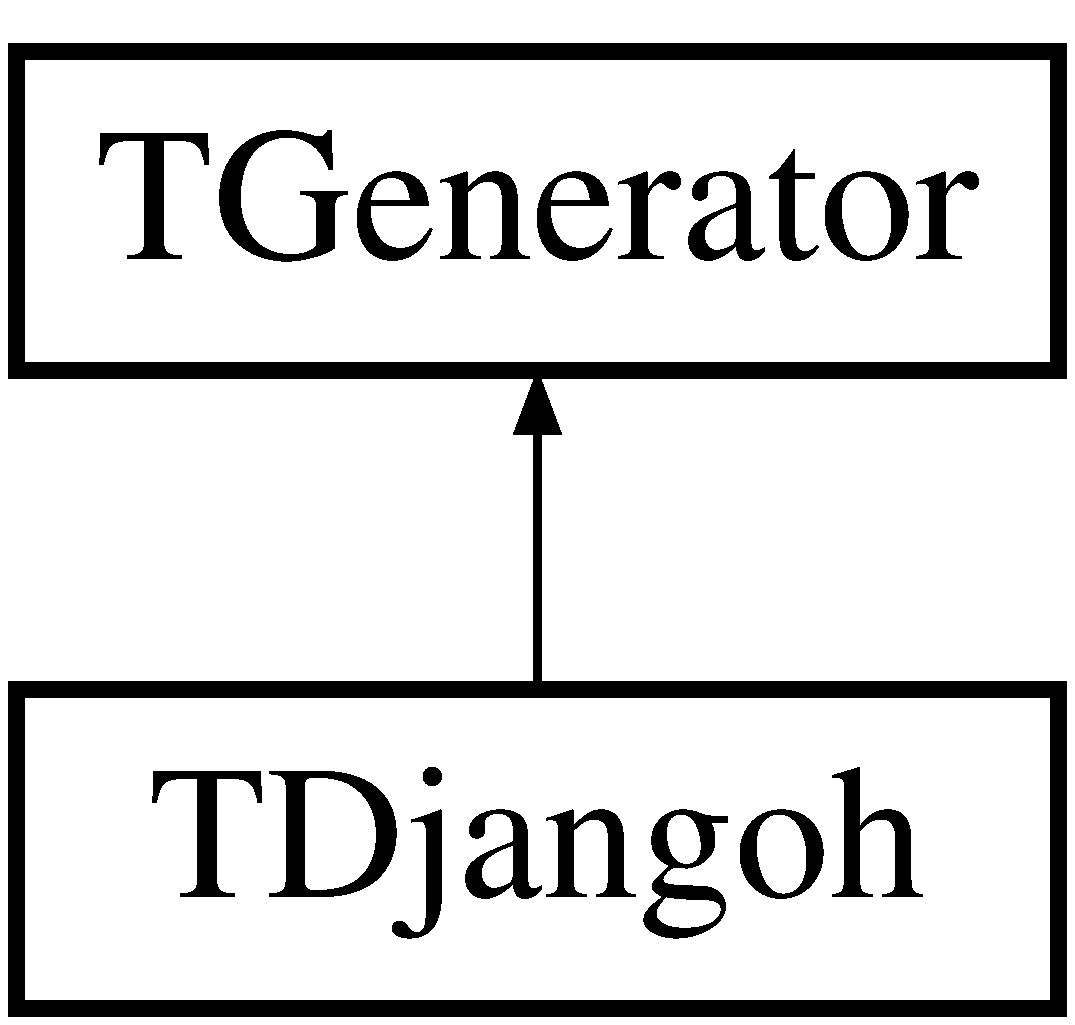
\includegraphics[height=2.000000cm]{class_t_djangoh}
\end{center}
\end{figure}
\subsection*{Classes}
\begin{DoxyCompactItemize}
\item 
class \hyperlink{class_t_djangoh_1_1_t_djangoh_cleaner}{T\+Djangoh\+Cleaner}
\begin{DoxyCompactList}\small\item\em A cleaner for \hyperlink{class_t_djangoh}{T\+Djangoh}. \end{DoxyCompactList}\end{DoxyCompactItemize}
\subsection*{Public Member Functions}
\begin{DoxyCompactItemize}
\item 
\hyperlink{class_t_djangoh_a7cbbb76ddc4fe82e25bb1e58078e45bc}{T\+Djangoh} ()
\begin{DoxyCompactList}\small\item\em Constructor of the \hyperlink{class_t_djangoh}{T\+Djangoh} class. \end{DoxyCompactList}\item 
virtual \hyperlink{class_t_djangoh_abee806f1e4536b30624590e34869f0e0}{$\sim$\+T\+Djangoh} ()
\begin{DoxyCompactList}\small\item\em Destructor of the \hyperlink{class_t_djangoh}{T\+Djangoh} class. \end{DoxyCompactList}\item 
void \hyperlink{class_t_djangoh_a121effe35c3f3ac168a4663bcd5eef5c}{Generate\+Event} ()
\begin{DoxyCompactList}\small\item\em Generation of an event. \end{DoxyCompactList}\item 
void \hyperlink{class_t_djangoh_a763cae78834404166df26ccd059bb301}{Initialize} ()
\begin{DoxyCompactList}\small\item\em Initialization of D\+J\+A\+N\+G\+OH. \end{DoxyCompactList}\item 
void \hyperlink{class_t_djangoh_af6954bed103bc5adc60822f16268c12d}{Read\+X\+M\+L\+File} (const string p\+Filename)
\begin{DoxyCompactList}\small\item\em Reading of parameters in X\+ML file. \end{DoxyCompactList}\item 
void \hyperlink{class_t_djangoh_ade135fa317b5678c048d417fcef573ae}{Write\+X\+M\+L\+File} (const string p\+Filename)
\item 
void \hyperlink{class_t_djangoh_a20fbc4c9736f639e6211333c6113421a}{Mod\+Kine\+Cuts} (int pcut, double pxmin, double pxmax, double pymin, double pymax, double pq2min, double pq2max, double pwmin)
\begin{DoxyCompactList}\small\item\em Modification of kinematical cuts. \end{DoxyCompactList}\item 
void \hyperlink{class_t_djangoh_acbf402e049af75c65f28589178eb1487}{Born\+W\+Oqel\+NC} ()
\begin{DoxyCompactList}\small\item\em Configuration for Born w/o quasielastic contribution generation. \end{DoxyCompactList}\item 
void \hyperlink{class_t_djangoh_a283b09ffc625a6a14af2f301ae957c92}{R\+Clep\+W\+Oqel\+NC} ()
\begin{DoxyCompactList}\small\item\em Configuration for leptonic RC w/o quasielastic contribution generation. \end{DoxyCompactList}\item 
void \hyperlink{class_t_djangoh_af58a4c6bb944a4ce79cc538829e490e8}{Configure} (float beam\+\_\+e, float pol)
\begin{DoxyCompactList}\small\item\em Configuration of D\+J\+A\+N\+G\+OH. \end{DoxyCompactList}\item 
void \hyperlink{class_t_djangoh_a076cac82063ed8740ac0a32e77c02c94}{End\+Recap} ()
\begin{DoxyCompactList}\small\item\em Print a recap of the generation made. \end{DoxyCompactList}\item 
Int\+\_\+t \hyperlink{class_t_djangoh_a69e5ebe63faa2dd00d9bcd217ecdf825}{Import\+Particles} (T\+Clones\+Array $\ast$particles, Option\+\_\+t $\ast$option=\char`\"{}\char`\"{})
\begin{DoxyCompactList}\small\item\em Import particles from lujets\+\_\+ subroutine and copy it in T\+Clones\+Array$\ast$. \end{DoxyCompactList}\item 
T\+Obj\+Array $\ast$ \hyperlink{class_t_djangoh_ac63f2c463b6a2fff98f256952aaf945f}{Import\+Particles} (Option\+\_\+t $\ast$option=\char`\"{}\char`\"{})
\begin{DoxyCompactList}\small\item\em Import particles from lujets\+\_\+ subroutine and copy it in T\+Clones\+Array$\ast$. \end{DoxyCompactList}\item 
double \hyperlink{class_t_djangoh_a6c3ac520ed9c8c8eb0e80f3dda7eb146}{Get\+Sigtot} ()
\begin{DoxyCompactList}\small\item\em Access total Cross-\/\+Section. \end{DoxyCompactList}\item 
double \hyperlink{class_t_djangoh_af888193a486499c7b019b0da80eae760}{Get\+Sigtrr} ()
\begin{DoxyCompactList}\small\item\em Access error on Cross-\/\+Section. \end{DoxyCompactList}\item 
int \hyperlink{class_t_djangoh_a2ed9a38fa1593d5a6a6e2c33b2912d1b}{Get\+Beam\+Type} ()
\begin{DoxyCompactList}\small\item\em Access beam particle type. \end{DoxyCompactList}\item 
void \hyperlink{class_t_djangoh_af93ae6412c07af22bca887cbcbba5082}{Set\+Beam\+Type} (int pvalue)
\begin{DoxyCompactList}\small\item\em Set beam particle type. \end{DoxyCompactList}\item 
void \hyperlink{class_t_djangoh_a37c2f8994175d3181a7f6f5aae5797f1}{Set\+Beam\+Type} (const char $\ast$pvalue)
\begin{DoxyCompactList}\small\item\em Set beam particle type. \end{DoxyCompactList}\item 
void \hyperlink{class_t_djangoh_a6995df5cd413a9e998fe8c0836004363}{Set\+Beam} (double p\+BeamE, double p\+Pol)
\begin{DoxyCompactList}\small\item\em Set beam energy and polarization. \end{DoxyCompactList}\item 
double \hyperlink{class_t_djangoh_a62b52fce9e36c0c7296fc1e519b1b902}{Get\+Beam\+Polar} ()
\begin{DoxyCompactList}\small\item\em Access beam polarization. \end{DoxyCompactList}\item 
double \hyperlink{class_t_djangoh_a34a0415a20f61670164665904eeca25b}{Set\+Beam\+Polar} (double pvalue)
\begin{DoxyCompactList}\small\item\em Set beam polarization. \end{DoxyCompactList}\item 
double \hyperlink{class_t_djangoh_a6baf26c760e0fc2f7bfc802fe7b14093}{Get\+Kinem\+Cut} (int i)
\begin{DoxyCompactList}\small\item\em Access kinematical cuts. \end{DoxyCompactList}\item 
void \hyperlink{class_t_djangoh_acb1c8c1ead16a0fbadd733b117cc0445}{Set\+Kinem\+Cut} (double pvalue, int i)
\begin{DoxyCompactList}\small\item\em Set kinematical cuts. \end{DoxyCompactList}\item 
double \hyperlink{class_t_djangoh_a74a77949c408cc303ec5e90482b1e639}{Get\+Gd\+Opt} (int i)
\begin{DoxyCompactList}\small\item\em Access cross-\/section grid values. \end{DoxyCompactList}\item 
void \hyperlink{class_t_djangoh_abbbe8452bf4a894e8757e096fb104d90}{Set\+Gd\+Opt} (double pvalue, int i)
\begin{DoxyCompactList}\small\item\em Set cross-\/section grid values. \end{DoxyCompactList}\item 
int \hyperlink{class_t_djangoh_ac58587b988731552d41321364c30748d}{Get\+Gsw} (int i)
\begin{DoxyCompactList}\small\item\em Access EW parameters values. \end{DoxyCompactList}\item 
void \hyperlink{class_t_djangoh_acbd9827496878eed7768c97031a1c1d7}{Set\+Gsw} (int pvalue, int i)
\begin{DoxyCompactList}\small\item\em Set EW parameters values. \end{DoxyCompactList}\item 
double \hyperlink{class_t_djangoh_a47b4a219c93cbcad58a82bfab9649a42}{Get\+Egam\+Min} ()
\begin{DoxyCompactList}\small\item\em Access cutoff energy value. \end{DoxyCompactList}\item 
void \hyperlink{class_t_djangoh_ac296a00fee7971d387aa5127f726a649}{Set\+Egam\+Min} (double pvalue)
\begin{DoxyCompactList}\small\item\em Set cutoff energy value. \end{DoxyCompactList}\item 
int \hyperlink{class_t_djangoh_aea74b082287a6870a27b07217832768f}{Get\+Int\+Opt\+NC} (int i)
\begin{DoxyCompactList}\small\item\em Access contribution to NC interactions values. \end{DoxyCompactList}\item 
void \hyperlink{class_t_djangoh_a867c7f0d6deb79773b4529e496a2ee23}{Set\+Int\+Opt\+NC} (int pvalue, int i)
\begin{DoxyCompactList}\small\item\em Set contribution to NC interactions values. \end{DoxyCompactList}\item 
void \hyperlink{class_t_djangoh_a6e6fa7e1826bd4e86be44d80a6bd6854}{Set\+Sam\+Opt\+NC} (int pvalue, int i)
\begin{DoxyCompactList}\small\item\em Set inclusion of NC cross-\/section to sampling values. \end{DoxyCompactList}\item 
int \hyperlink{class_t_djangoh_a58e1925539d208ca8e00533b5ae52074}{Get\+Struct\+Func} (int i)
\begin{DoxyCompactList}\small\item\em Access parametrization of structure functions values. \end{DoxyCompactList}\item 
void \hyperlink{class_t_djangoh_aa8331885aeb7880a63ebdfcf32919f9b}{Set\+Struct\+Func} (int pvalue, int i)
\begin{DoxyCompactList}\small\item\em Set parametrization of structure functions values. \end{DoxyCompactList}\item 
double \hyperlink{class_t_djangoh_a31acc70811ad58a8986f7d04547e9213}{Get\+Sophia} ()
\begin{DoxyCompactList}\small\item\em Access low W limit for Sophia value. \end{DoxyCompactList}\item 
void \hyperlink{class_t_djangoh_a12bd5515ab5db50b147810e06e98a0b8}{Set\+Sophia} (double pvalue)
\begin{DoxyCompactList}\small\item\em Set low W limit for Sophia value. \end{DoxyCompactList}\item 
int \hyperlink{class_t_djangoh_a1caf80b8f7228dbc7818ac047de9b8b7}{Get\+Verbose} ()
\begin{DoxyCompactList}\small\item\em Get verbose value. \end{DoxyCompactList}\item 
void \hyperlink{class_t_djangoh_a5129257c110777c1625049fb74f33e4b}{Set\+Verbose} (int pvalue)
\begin{DoxyCompactList}\small\item\em Set verbose value. \end{DoxyCompactList}\item 
int \hyperlink{class_t_djangoh_a39b356c5689222e6c82172e9b4954fe1}{Get\+Int\+Opt\+CC} (int i)
\begin{DoxyCompactList}\small\item\em Access contribution to CC interactions values. \end{DoxyCompactList}\item 
void \hyperlink{class_t_djangoh_a7e37a7afc5c112a2bd061f5e73973f78}{Set\+Int\+Opt\+CC} (int pvalue, int i)
\begin{DoxyCompactList}\small\item\em Set contribution to CC interactions values. \end{DoxyCompactList}\item 
void \hyperlink{class_t_djangoh_acc7a3124293fe30c297fb7702bade781}{Set\+Sam\+Opt\+CC} (int pvalue, int i)
\begin{DoxyCompactList}\small\item\em Set inclusion of CC cross-\/section to sampling values. \end{DoxyCompactList}\item 
void \hyperlink{class_t_djangoh_ae37cb56d62427ac672155e0817f6849e}{Set\+Nucleus} (double p\+Hpolar, int p\+Hna, int p\+Hnz, double p\+Epro=0)
\begin{DoxyCompactList}\small\item\em Set nucleus properties values. \end{DoxyCompactList}\item 
void \hyperlink{class_t_djangoh_aa78f3a43ed71499a9efe9e87cc22d668}{Write\+F\+S\+In\+File} ()
\begin{DoxyCompactList}\small\item\em Save final state infos in file. \end{DoxyCompactList}\item 
void \hyperlink{class_t_djangoh_ade1e9ff8b29d2b95d24a22c3474a7ba6}{Clean\+F\+S\+File} ()
\begin{DoxyCompactList}\small\item\em Remove final state file. \end{DoxyCompactList}\item 
double \hyperlink{class_t_djangoh_acf17f3e8d6a10ebe25f57f75662a1817}{Get\+P\+H\+EP} (int ip, int i)
\begin{DoxyCompactList}\small\item\em Access P\+H\+EP content of event. \end{DoxyCompactList}\item 
double \hyperlink{class_t_djangoh_ab8bbab97c50a6a9f296fbd0d78e98e17}{Get\+V\+H\+KK} (int ip, int i)
\begin{DoxyCompactList}\small\item\em Access V\+H\+KK content of event. \end{DoxyCompactList}\item 
int \hyperlink{class_t_djangoh_aaa275337568bcd47d87a63f1de688d27}{Get\+I\+D\+P\+H\+EP} (int i)
\begin{DoxyCompactList}\small\item\em Access I\+D\+P\+H\+EP content of event. \end{DoxyCompactList}\item 
int \hyperlink{class_t_djangoh_a381b6da1d6ef7145d9b4e49afb44a654}{Get\+Channel} ()
\begin{DoxyCompactList}\small\item\em Access sampling channel from Djangoh. \end{DoxyCompactList}\item 
void \hyperlink{class_t_djangoh_adf5acc5294013735f2475d4ce8ccf012}{Clean\+\_\+\+File} ()
\begin{DoxyCompactList}\small\item\em Clean files created by djangoh. \end{DoxyCompactList}\item 
\hyperlink{struct_lujets__t}{Lujets\+\_\+t} $\ast$ \hyperlink{class_t_djangoh_a2572e682379a304f84f21840d488fa0c}{Get\+Lujets} ()
\begin{DoxyCompactList}\small\item\em Recover the actual \hyperlink{struct_lujets__t}{Lujets\+\_\+t} structure. \end{DoxyCompactList}\item 
int \hyperlink{class_t_djangoh_a501e50bbb1ad6a75014fd7c555313b74}{GetN} ()
\begin{DoxyCompactList}\small\item\em Recover the number of particles. \end{DoxyCompactList}\item 
int \hyperlink{class_t_djangoh_afb58be11a10e8a6a4b442ea0fe4e16f5}{Get\+N\+P\+AD} ()
\begin{DoxyCompactList}\small\item\em Recover. \end{DoxyCompactList}\item 
int \hyperlink{class_t_djangoh_aaf2c94dbb8382bbd3b7ed1530a8ac878}{GetK} (int ip, int i)
\begin{DoxyCompactList}\small\item\em Access K content of event. \end{DoxyCompactList}\item 
double \hyperlink{class_t_djangoh_a2bc14d05d493e604f9f7fef847c19c9b}{GetP} (int ip, int i)
\begin{DoxyCompactList}\small\item\em Access P content of event. \end{DoxyCompactList}\item 
double \hyperlink{class_t_djangoh_a4993a87fef8917b9ed8a55811aa2daf6}{GetV} (int ip, int i)
\begin{DoxyCompactList}\small\item\em Access V content of event. \end{DoxyCompactList}\item 
void \hyperlink{class_t_djangoh_ac15b9862e954349fd9f0911c71e0e664}{SetN} (int n)
\begin{DoxyCompactList}\small\item\em Set the number of particles. \end{DoxyCompactList}\item 
void \hyperlink{class_t_djangoh_a0ed7bb7e7433a6385b5838ce519168a2}{Set\+N\+P\+AD} (int n)
\begin{DoxyCompactList}\small\item\em Set N\+P\+AD. \end{DoxyCompactList}\item 
void \hyperlink{class_t_djangoh_a045a7fabe350589453e240bff98ca54b}{SetK} (int ip, int i, int k)
\begin{DoxyCompactList}\small\item\em Set K content of event. \end{DoxyCompactList}\item 
void \hyperlink{class_t_djangoh_aa9cfa62ac6bf01a7f5214cc62cdae34c}{SetP} (int ip, int i, double p)
\begin{DoxyCompactList}\small\item\em Set P content of event. \end{DoxyCompactList}\item 
void \hyperlink{class_t_djangoh_a472e228f316f1473c940dfa37c22637c}{SetV} (int ip, int i, double v)
\begin{DoxyCompactList}\small\item\em Set V content of event. \end{DoxyCompactList}\item 
\hyperlink{struct_djkin__t}{Djkin\+\_\+t} $\ast$ \hyperlink{class_t_djangoh_a4f5a22f9af97e7c84660c94cd354f780}{Get\+Djkin} ()
\item 
double \hyperlink{class_t_djangoh_aa2d4a28a97826cf32b9d623c581da9de}{GetX} ()
\item 
double \hyperlink{class_t_djangoh_aee089d5536e8acb68236f9546e4f06e2}{GetY} ()
\item 
double \hyperlink{class_t_djangoh_a94c252e7c5375e9641ad5ea048098c06}{Get\+W2} ()
\item 
double \hyperlink{class_t_djangoh_afce6f0bfed90b20eb0f9310ae107291d}{Get\+Q2} ()
\item 
double \hyperlink{class_t_djangoh_a6e69090ac8581a1be96cac889cf5292b}{GetU} ()
\item 
double \hyperlink{class_t_djangoh_a64b580157191cf32f0b3ba4047b69bdf}{Get\+X\+H\+AD} ()
\item 
double \hyperlink{class_t_djangoh_a4cfb37ad76ec038f6e05b90341befb7f}{Get\+Y\+H\+AD} ()
\item 
double \hyperlink{class_t_djangoh_a969e748da53637a3732a27cfe23a34d2}{Get\+Q2\+H\+AD} ()
\item 
void \hyperlink{class_t_djangoh_a1ef3828a15dfd67a5e5c902bd584fd8b}{SetX} (double x)
\item 
void \hyperlink{class_t_djangoh_a91061fe2a386a9ddb7c7398c9443fa74}{SetY} (double y)
\item 
void \hyperlink{class_t_djangoh_aea9a499dfc8cbca480f228b79a05d99a}{Set\+W2} (double w)
\item 
void \hyperlink{class_t_djangoh_abecf2835ceecd72f0847544b72fd837e}{Set\+Q2} (double q)
\item 
void \hyperlink{class_t_djangoh_a69cebdc5dc26bfd0def872a996da0650}{SetU} (double u)
\item 
void \hyperlink{class_t_djangoh_a13173ef3490a98d8488ce7421905284c}{Set\+X\+H\+AD} (double x)
\item 
void \hyperlink{class_t_djangoh_a2dc4b62cd66dd41e8ae3d62965e36617}{Set\+Y\+H\+AD} (double y)
\item 
void \hyperlink{class_t_djangoh_a0066b103b2f779d8ed302fd77f42ee5e}{Set\+Q2\+H\+AD} (double q)
\end{DoxyCompactItemize}
\subsection*{Static Public Member Functions}
\begin{DoxyCompactItemize}
\item 
static \hyperlink{class_t_djangoh}{T\+Djangoh} $\ast$ \hyperlink{class_t_djangoh_a2e9871b8bec6326bb518f218dc87402c}{Instance} ()
\begin{DoxyCompactList}\small\item\em Instance creation. \end{DoxyCompactList}\end{DoxyCompactItemize}
\subsection*{Protected Member Functions}
\begin{DoxyCompactItemize}
\item 
\hyperlink{class_t_djangoh_a7b47ea508e2047b99b6f3efd6ba37278}{T\+Djangoh} (const \hyperlink{class_t_djangoh}{T\+Djangoh} \&)
\begin{DoxyCompactList}\small\item\em Copy Constructor of the \hyperlink{class_t_djangoh}{T\+Djangoh} class. \end{DoxyCompactList}\item 
\hyperlink{class_t_djangoh}{T\+Djangoh} \& \hyperlink{class_t_djangoh_a987204dc283979db28c83e5a35177b7c}{operator=} (const \hyperlink{class_t_djangoh}{T\+Djangoh} \&)
\begin{DoxyCompactList}\small\item\em = operator overload \end{DoxyCompactList}\end{DoxyCompactItemize}
\subsection*{Protected Attributes}
\begin{DoxyCompactItemize}
\item 
\hyperlink{struct_lujets__t}{Lujets\+\_\+t} $\ast$ \hyperlink{class_t_djangoh_a844cd27abcd743028fb98b3fba0c0fa9}{f\+Lujets}
\item 
\hyperlink{struct_djkin__t}{Djkin\+\_\+t} $\ast$ \hyperlink{class_t_djangoh_a870f9e5b91afdae5f21c10daae7c5d7e}{f\+Djkin}
\end{DoxyCompactItemize}
\subsection*{Static Protected Attributes}
\begin{DoxyCompactItemize}
\item 
static \hyperlink{class_t_djangoh}{T\+Djangoh} $\ast$ \hyperlink{class_t_djangoh_ad154e9fce28f84ab490dc6508db58fb8}{fg\+Instance} = 0
\end{DoxyCompactItemize}


\subsection{Detailed Description}
C/\+C++ Interface to Djangoh. 

\subsection{Constructor \& Destructor Documentation}
\mbox{\Hypertarget{class_t_djangoh_a7b47ea508e2047b99b6f3efd6ba37278}\label{class_t_djangoh_a7b47ea508e2047b99b6f3efd6ba37278}} 
\index{T\+Djangoh@{T\+Djangoh}!T\+Djangoh@{T\+Djangoh}}
\index{T\+Djangoh@{T\+Djangoh}!T\+Djangoh@{T\+Djangoh}}
\subsubsection{\texorpdfstring{T\+Djangoh()}{TDjangoh()}\hspace{0.1cm}{\footnotesize\ttfamily [1/2]}}
{\footnotesize\ttfamily T\+Djangoh\+::\+T\+Djangoh (\begin{DoxyParamCaption}\item[{const \hyperlink{class_t_djangoh}{T\+Djangoh} \&}]{dj }\end{DoxyParamCaption})\hspace{0.3cm}{\ttfamily [protected]}}



Copy Constructor of the \hyperlink{class_t_djangoh}{T\+Djangoh} class. 


\begin{DoxyParams}{Parameters}
{\em \hyperlink{class_t_djangoh}{T\+Djangoh}} & \+: \hyperlink{class_t_djangoh}{T\+Djangoh} object \\
\hline
\end{DoxyParams}
\mbox{\Hypertarget{class_t_djangoh_a7cbbb76ddc4fe82e25bb1e58078e45bc}\label{class_t_djangoh_a7cbbb76ddc4fe82e25bb1e58078e45bc}} 
\index{T\+Djangoh@{T\+Djangoh}!T\+Djangoh@{T\+Djangoh}}
\index{T\+Djangoh@{T\+Djangoh}!T\+Djangoh@{T\+Djangoh}}
\subsubsection{\texorpdfstring{T\+Djangoh()}{TDjangoh()}\hspace{0.1cm}{\footnotesize\ttfamily [2/2]}}
{\footnotesize\ttfamily T\+Djangoh\+::\+T\+Djangoh (\begin{DoxyParamCaption}{ }\end{DoxyParamCaption})}



Constructor of the \hyperlink{class_t_djangoh}{T\+Djangoh} class. 

\mbox{\Hypertarget{class_t_djangoh_abee806f1e4536b30624590e34869f0e0}\label{class_t_djangoh_abee806f1e4536b30624590e34869f0e0}} 
\index{T\+Djangoh@{T\+Djangoh}!````~T\+Djangoh@{$\sim$\+T\+Djangoh}}
\index{````~T\+Djangoh@{$\sim$\+T\+Djangoh}!T\+Djangoh@{T\+Djangoh}}
\subsubsection{\texorpdfstring{$\sim$\+T\+Djangoh()}{~TDjangoh()}}
{\footnotesize\ttfamily T\+Djangoh\+::$\sim$\+T\+Djangoh (\begin{DoxyParamCaption}{ }\end{DoxyParamCaption})\hspace{0.3cm}{\ttfamily [virtual]}}



Destructor of the \hyperlink{class_t_djangoh}{T\+Djangoh} class. 



\subsection{Member Function Documentation}
\mbox{\Hypertarget{class_t_djangoh_acbf402e049af75c65f28589178eb1487}\label{class_t_djangoh_acbf402e049af75c65f28589178eb1487}} 
\index{T\+Djangoh@{T\+Djangoh}!Born\+W\+Oqel\+NC@{Born\+W\+Oqel\+NC}}
\index{Born\+W\+Oqel\+NC@{Born\+W\+Oqel\+NC}!T\+Djangoh@{T\+Djangoh}}
\subsubsection{\texorpdfstring{Born\+W\+Oqel\+N\+C()}{BornWOqelNC()}}
{\footnotesize\ttfamily void T\+Djangoh\+::\+Born\+W\+Oqel\+NC (\begin{DoxyParamCaption}{ }\end{DoxyParamCaption})}



Configuration for Born w/o quasielastic contribution generation. 

\mbox{\Hypertarget{class_t_djangoh_adf5acc5294013735f2475d4ce8ccf012}\label{class_t_djangoh_adf5acc5294013735f2475d4ce8ccf012}} 
\index{T\+Djangoh@{T\+Djangoh}!Clean\+\_\+\+File@{Clean\+\_\+\+File}}
\index{Clean\+\_\+\+File@{Clean\+\_\+\+File}!T\+Djangoh@{T\+Djangoh}}
\subsubsection{\texorpdfstring{Clean\+\_\+\+File()}{Clean\_File()}}
{\footnotesize\ttfamily void T\+Djangoh\+::\+Clean\+\_\+\+File (\begin{DoxyParamCaption}{ }\end{DoxyParamCaption})}



Clean files created by djangoh. 

\mbox{\Hypertarget{class_t_djangoh_ade1e9ff8b29d2b95d24a22c3474a7ba6}\label{class_t_djangoh_ade1e9ff8b29d2b95d24a22c3474a7ba6}} 
\index{T\+Djangoh@{T\+Djangoh}!Clean\+F\+S\+File@{Clean\+F\+S\+File}}
\index{Clean\+F\+S\+File@{Clean\+F\+S\+File}!T\+Djangoh@{T\+Djangoh}}
\subsubsection{\texorpdfstring{Clean\+F\+S\+File()}{CleanFSFile()}}
{\footnotesize\ttfamily void T\+Djangoh\+::\+Clean\+F\+S\+File (\begin{DoxyParamCaption}{ }\end{DoxyParamCaption})\hspace{0.3cm}{\ttfamily [inline]}}



Remove final state file. 

\mbox{\Hypertarget{class_t_djangoh_af58a4c6bb944a4ce79cc538829e490e8}\label{class_t_djangoh_af58a4c6bb944a4ce79cc538829e490e8}} 
\index{T\+Djangoh@{T\+Djangoh}!Configure@{Configure}}
\index{Configure@{Configure}!T\+Djangoh@{T\+Djangoh}}
\subsubsection{\texorpdfstring{Configure()}{Configure()}}
{\footnotesize\ttfamily void T\+Djangoh\+::\+Configure (\begin{DoxyParamCaption}\item[{float}]{beam\+\_\+e,  }\item[{float}]{pol }\end{DoxyParamCaption})}



Configuration of D\+J\+A\+N\+G\+OH. 


\begin{DoxyParams}{Parameters}
{\em beam\+\_\+e} & \+: Energy of the beam (in GeV) \\
\hline
\end{DoxyParams}
\mbox{\Hypertarget{class_t_djangoh_a076cac82063ed8740ac0a32e77c02c94}\label{class_t_djangoh_a076cac82063ed8740ac0a32e77c02c94}} 
\index{T\+Djangoh@{T\+Djangoh}!End\+Recap@{End\+Recap}}
\index{End\+Recap@{End\+Recap}!T\+Djangoh@{T\+Djangoh}}
\subsubsection{\texorpdfstring{End\+Recap()}{EndRecap()}}
{\footnotesize\ttfamily void T\+Djangoh\+::\+End\+Recap (\begin{DoxyParamCaption}{ }\end{DoxyParamCaption})}



Print a recap of the generation made. 

\mbox{\Hypertarget{class_t_djangoh_a121effe35c3f3ac168a4663bcd5eef5c}\label{class_t_djangoh_a121effe35c3f3ac168a4663bcd5eef5c}} 
\index{T\+Djangoh@{T\+Djangoh}!Generate\+Event@{Generate\+Event}}
\index{Generate\+Event@{Generate\+Event}!T\+Djangoh@{T\+Djangoh}}
\subsubsection{\texorpdfstring{Generate\+Event()}{GenerateEvent()}}
{\footnotesize\ttfamily void T\+Djangoh\+::\+Generate\+Event (\begin{DoxyParamCaption}{ }\end{DoxyParamCaption})}



Generation of an event. 

\mbox{\Hypertarget{class_t_djangoh_a62b52fce9e36c0c7296fc1e519b1b902}\label{class_t_djangoh_a62b52fce9e36c0c7296fc1e519b1b902}} 
\index{T\+Djangoh@{T\+Djangoh}!Get\+Beam\+Polar@{Get\+Beam\+Polar}}
\index{Get\+Beam\+Polar@{Get\+Beam\+Polar}!T\+Djangoh@{T\+Djangoh}}
\subsubsection{\texorpdfstring{Get\+Beam\+Polar()}{GetBeamPolar()}}
{\footnotesize\ttfamily double T\+Djangoh\+::\+Get\+Beam\+Polar (\begin{DoxyParamCaption}{ }\end{DoxyParamCaption})}



Access beam polarization. 

\begin{DoxyReturn}{Returns}
Beam polarization 
\end{DoxyReturn}
\mbox{\Hypertarget{class_t_djangoh_a2ed9a38fa1593d5a6a6e2c33b2912d1b}\label{class_t_djangoh_a2ed9a38fa1593d5a6a6e2c33b2912d1b}} 
\index{T\+Djangoh@{T\+Djangoh}!Get\+Beam\+Type@{Get\+Beam\+Type}}
\index{Get\+Beam\+Type@{Get\+Beam\+Type}!T\+Djangoh@{T\+Djangoh}}
\subsubsection{\texorpdfstring{Get\+Beam\+Type()}{GetBeamType()}}
{\footnotesize\ttfamily int T\+Djangoh\+::\+Get\+Beam\+Type (\begin{DoxyParamCaption}{ }\end{DoxyParamCaption})}



Access beam particle type. 

\begin{DoxyReturn}{Returns}
Beam particle type 
\end{DoxyReturn}
\mbox{\Hypertarget{class_t_djangoh_a381b6da1d6ef7145d9b4e49afb44a654}\label{class_t_djangoh_a381b6da1d6ef7145d9b4e49afb44a654}} 
\index{T\+Djangoh@{T\+Djangoh}!Get\+Channel@{Get\+Channel}}
\index{Get\+Channel@{Get\+Channel}!T\+Djangoh@{T\+Djangoh}}
\subsubsection{\texorpdfstring{Get\+Channel()}{GetChannel()}}
{\footnotesize\ttfamily int T\+Djangoh\+::\+Get\+Channel (\begin{DoxyParamCaption}{ }\end{DoxyParamCaption})}



Access sampling channel from Djangoh. 

\begin{DoxyReturn}{Returns}
Sampling channel number 
\end{DoxyReturn}
\mbox{\Hypertarget{class_t_djangoh_a4f5a22f9af97e7c84660c94cd354f780}\label{class_t_djangoh_a4f5a22f9af97e7c84660c94cd354f780}} 
\index{T\+Djangoh@{T\+Djangoh}!Get\+Djkin@{Get\+Djkin}}
\index{Get\+Djkin@{Get\+Djkin}!T\+Djangoh@{T\+Djangoh}}
\subsubsection{\texorpdfstring{Get\+Djkin()}{GetDjkin()}}
{\footnotesize\ttfamily \hyperlink{struct_djkin__t}{Djkin\+\_\+t}$\ast$ T\+Djangoh\+::\+Get\+Djkin (\begin{DoxyParamCaption}{ }\end{DoxyParamCaption})\hspace{0.3cm}{\ttfamily [inline]}}

\mbox{\Hypertarget{class_t_djangoh_a47b4a219c93cbcad58a82bfab9649a42}\label{class_t_djangoh_a47b4a219c93cbcad58a82bfab9649a42}} 
\index{T\+Djangoh@{T\+Djangoh}!Get\+Egam\+Min@{Get\+Egam\+Min}}
\index{Get\+Egam\+Min@{Get\+Egam\+Min}!T\+Djangoh@{T\+Djangoh}}
\subsubsection{\texorpdfstring{Get\+Egam\+Min()}{GetEgamMin()}}
{\footnotesize\ttfamily double T\+Djangoh\+::\+Get\+Egam\+Min (\begin{DoxyParamCaption}{ }\end{DoxyParamCaption})}



Access cutoff energy value. 

\begin{DoxyReturn}{Returns}
Cutoff energy value 
\end{DoxyReturn}
\mbox{\Hypertarget{class_t_djangoh_a74a77949c408cc303ec5e90482b1e639}\label{class_t_djangoh_a74a77949c408cc303ec5e90482b1e639}} 
\index{T\+Djangoh@{T\+Djangoh}!Get\+Gd\+Opt@{Get\+Gd\+Opt}}
\index{Get\+Gd\+Opt@{Get\+Gd\+Opt}!T\+Djangoh@{T\+Djangoh}}
\subsubsection{\texorpdfstring{Get\+Gd\+Opt()}{GetGdOpt()}}
{\footnotesize\ttfamily double T\+Djangoh\+::\+Get\+Gd\+Opt (\begin{DoxyParamCaption}\item[{int}]{i }\end{DoxyParamCaption})}



Access cross-\/section grid values. 


\begin{DoxyParams}{Parameters}
{\em i} & \+: Cross-\/section grid value number (in the order as in the manual) \\
\hline
\end{DoxyParams}
\begin{DoxyReturn}{Returns}
Cross-\/section grid value 
\end{DoxyReturn}
\mbox{\Hypertarget{class_t_djangoh_ac58587b988731552d41321364c30748d}\label{class_t_djangoh_ac58587b988731552d41321364c30748d}} 
\index{T\+Djangoh@{T\+Djangoh}!Get\+Gsw@{Get\+Gsw}}
\index{Get\+Gsw@{Get\+Gsw}!T\+Djangoh@{T\+Djangoh}}
\subsubsection{\texorpdfstring{Get\+Gsw()}{GetGsw()}}
{\footnotesize\ttfamily int T\+Djangoh\+::\+Get\+Gsw (\begin{DoxyParamCaption}\item[{int}]{i }\end{DoxyParamCaption})}



Access EW parameters values. 


\begin{DoxyParams}{Parameters}
{\em i} & \+: EW parameter value number (in the order as in the manual) \\
\hline
\end{DoxyParams}
\begin{DoxyReturn}{Returns}
EW parameter value 
\end{DoxyReturn}
\mbox{\Hypertarget{class_t_djangoh_aaa275337568bcd47d87a63f1de688d27}\label{class_t_djangoh_aaa275337568bcd47d87a63f1de688d27}} 
\index{T\+Djangoh@{T\+Djangoh}!Get\+I\+D\+P\+H\+EP@{Get\+I\+D\+P\+H\+EP}}
\index{Get\+I\+D\+P\+H\+EP@{Get\+I\+D\+P\+H\+EP}!T\+Djangoh@{T\+Djangoh}}
\subsubsection{\texorpdfstring{Get\+I\+D\+P\+H\+E\+P()}{GetIDPHEP()}}
{\footnotesize\ttfamily int T\+Djangoh\+::\+Get\+I\+D\+P\+H\+EP (\begin{DoxyParamCaption}\item[{int}]{i }\end{DoxyParamCaption})}



Access I\+D\+P\+H\+EP content of event. 


\begin{DoxyParams}{Parameters}
{\em i} & \+: index \\
\hline
\end{DoxyParams}
\begin{DoxyReturn}{Returns}
I\+D\+P\+H\+E\+P(i) 
\end{DoxyReturn}
\mbox{\Hypertarget{class_t_djangoh_a39b356c5689222e6c82172e9b4954fe1}\label{class_t_djangoh_a39b356c5689222e6c82172e9b4954fe1}} 
\index{T\+Djangoh@{T\+Djangoh}!Get\+Int\+Opt\+CC@{Get\+Int\+Opt\+CC}}
\index{Get\+Int\+Opt\+CC@{Get\+Int\+Opt\+CC}!T\+Djangoh@{T\+Djangoh}}
\subsubsection{\texorpdfstring{Get\+Int\+Opt\+C\+C()}{GetIntOptCC()}}
{\footnotesize\ttfamily int T\+Djangoh\+::\+Get\+Int\+Opt\+CC (\begin{DoxyParamCaption}\item[{int}]{i }\end{DoxyParamCaption})}



Access contribution to CC interactions values. 


\begin{DoxyParams}{Parameters}
{\em i} & \+: Contribution value number (in the order as in the manual) \\
\hline
\end{DoxyParams}
\begin{DoxyReturn}{Returns}
Contribution value 
\end{DoxyReturn}
\mbox{\Hypertarget{class_t_djangoh_aea74b082287a6870a27b07217832768f}\label{class_t_djangoh_aea74b082287a6870a27b07217832768f}} 
\index{T\+Djangoh@{T\+Djangoh}!Get\+Int\+Opt\+NC@{Get\+Int\+Opt\+NC}}
\index{Get\+Int\+Opt\+NC@{Get\+Int\+Opt\+NC}!T\+Djangoh@{T\+Djangoh}}
\subsubsection{\texorpdfstring{Get\+Int\+Opt\+N\+C()}{GetIntOptNC()}}
{\footnotesize\ttfamily int T\+Djangoh\+::\+Get\+Int\+Opt\+NC (\begin{DoxyParamCaption}\item[{int}]{i }\end{DoxyParamCaption})}



Access contribution to NC interactions values. 


\begin{DoxyParams}{Parameters}
{\em i} & \+: Contribution value number (in the order as in the manual) \\
\hline
\end{DoxyParams}
\begin{DoxyReturn}{Returns}
Contribution value 
\end{DoxyReturn}
\mbox{\Hypertarget{class_t_djangoh_aaf2c94dbb8382bbd3b7ed1530a8ac878}\label{class_t_djangoh_aaf2c94dbb8382bbd3b7ed1530a8ac878}} 
\index{T\+Djangoh@{T\+Djangoh}!GetK@{GetK}}
\index{GetK@{GetK}!T\+Djangoh@{T\+Djangoh}}
\subsubsection{\texorpdfstring{Get\+K()}{GetK()}}
{\footnotesize\ttfamily int T\+Djangoh\+::\+GetK (\begin{DoxyParamCaption}\item[{int}]{ip,  }\item[{int}]{i }\end{DoxyParamCaption})\hspace{0.3cm}{\ttfamily [inline]}}



Access K content of event. 


\begin{DoxyParams}{Parameters}
{\em ip} & \+: column index \\
\hline
{\em i} & \+: row index \\
\hline
\end{DoxyParams}
\begin{DoxyReturn}{Returns}
K(ip,i) 
\end{DoxyReturn}
\mbox{\Hypertarget{class_t_djangoh_a6baf26c760e0fc2f7bfc802fe7b14093}\label{class_t_djangoh_a6baf26c760e0fc2f7bfc802fe7b14093}} 
\index{T\+Djangoh@{T\+Djangoh}!Get\+Kinem\+Cut@{Get\+Kinem\+Cut}}
\index{Get\+Kinem\+Cut@{Get\+Kinem\+Cut}!T\+Djangoh@{T\+Djangoh}}
\subsubsection{\texorpdfstring{Get\+Kinem\+Cut()}{GetKinemCut()}}
{\footnotesize\ttfamily double T\+Djangoh\+::\+Get\+Kinem\+Cut (\begin{DoxyParamCaption}\item[{int}]{i }\end{DoxyParamCaption})}



Access kinematical cuts. 


\begin{DoxyParams}{Parameters}
{\em i} & \+: Kinematical cut number (in the order as in the manual) \\
\hline
\end{DoxyParams}
\begin{DoxyReturn}{Returns}
Cut value 
\end{DoxyReturn}
\mbox{\Hypertarget{class_t_djangoh_a2572e682379a304f84f21840d488fa0c}\label{class_t_djangoh_a2572e682379a304f84f21840d488fa0c}} 
\index{T\+Djangoh@{T\+Djangoh}!Get\+Lujets@{Get\+Lujets}}
\index{Get\+Lujets@{Get\+Lujets}!T\+Djangoh@{T\+Djangoh}}
\subsubsection{\texorpdfstring{Get\+Lujets()}{GetLujets()}}
{\footnotesize\ttfamily \hyperlink{struct_lujets__t}{Lujets\+\_\+t}$\ast$ T\+Djangoh\+::\+Get\+Lujets (\begin{DoxyParamCaption}{ }\end{DoxyParamCaption})\hspace{0.3cm}{\ttfamily [inline]}}



Recover the actual \hyperlink{struct_lujets__t}{Lujets\+\_\+t} structure. 

\begin{DoxyReturn}{Returns}
f\+Lujets 
\end{DoxyReturn}
\mbox{\Hypertarget{class_t_djangoh_a501e50bbb1ad6a75014fd7c555313b74}\label{class_t_djangoh_a501e50bbb1ad6a75014fd7c555313b74}} 
\index{T\+Djangoh@{T\+Djangoh}!GetN@{GetN}}
\index{GetN@{GetN}!T\+Djangoh@{T\+Djangoh}}
\subsubsection{\texorpdfstring{Get\+N()}{GetN()}}
{\footnotesize\ttfamily int T\+Djangoh\+::\+GetN (\begin{DoxyParamCaption}{ }\end{DoxyParamCaption})\hspace{0.3cm}{\ttfamily [inline]}}



Recover the number of particles. 

\begin{DoxyReturn}{Returns}
N 
\end{DoxyReturn}
\mbox{\Hypertarget{class_t_djangoh_afb58be11a10e8a6a4b442ea0fe4e16f5}\label{class_t_djangoh_afb58be11a10e8a6a4b442ea0fe4e16f5}} 
\index{T\+Djangoh@{T\+Djangoh}!Get\+N\+P\+AD@{Get\+N\+P\+AD}}
\index{Get\+N\+P\+AD@{Get\+N\+P\+AD}!T\+Djangoh@{T\+Djangoh}}
\subsubsection{\texorpdfstring{Get\+N\+P\+A\+D()}{GetNPAD()}}
{\footnotesize\ttfamily int T\+Djangoh\+::\+Get\+N\+P\+AD (\begin{DoxyParamCaption}{ }\end{DoxyParamCaption})\hspace{0.3cm}{\ttfamily [inline]}}



Recover. 

\begin{DoxyReturn}{Returns}
N\+P\+AD 
\end{DoxyReturn}
\mbox{\Hypertarget{class_t_djangoh_a2bc14d05d493e604f9f7fef847c19c9b}\label{class_t_djangoh_a2bc14d05d493e604f9f7fef847c19c9b}} 
\index{T\+Djangoh@{T\+Djangoh}!GetP@{GetP}}
\index{GetP@{GetP}!T\+Djangoh@{T\+Djangoh}}
\subsubsection{\texorpdfstring{Get\+P()}{GetP()}}
{\footnotesize\ttfamily double T\+Djangoh\+::\+GetP (\begin{DoxyParamCaption}\item[{int}]{ip,  }\item[{int}]{i }\end{DoxyParamCaption})\hspace{0.3cm}{\ttfamily [inline]}}



Access P content of event. 


\begin{DoxyParams}{Parameters}
{\em ip} & \+: column index \\
\hline
{\em i} & \+: row index \\
\hline
\end{DoxyParams}
\begin{DoxyReturn}{Returns}
P(ip,i) 
\end{DoxyReturn}
\mbox{\Hypertarget{class_t_djangoh_acf17f3e8d6a10ebe25f57f75662a1817}\label{class_t_djangoh_acf17f3e8d6a10ebe25f57f75662a1817}} 
\index{T\+Djangoh@{T\+Djangoh}!Get\+P\+H\+EP@{Get\+P\+H\+EP}}
\index{Get\+P\+H\+EP@{Get\+P\+H\+EP}!T\+Djangoh@{T\+Djangoh}}
\subsubsection{\texorpdfstring{Get\+P\+H\+E\+P()}{GetPHEP()}}
{\footnotesize\ttfamily double T\+Djangoh\+::\+Get\+P\+H\+EP (\begin{DoxyParamCaption}\item[{int}]{ip,  }\item[{int}]{i }\end{DoxyParamCaption})}



Access P\+H\+EP content of event. 


\begin{DoxyParams}{Parameters}
{\em ip} & \+: Column index \\
\hline
{\em i} & \+: row index \\
\hline
\end{DoxyParams}
\begin{DoxyReturn}{Returns}
P\+H\+E\+P(ip,i) 
\end{DoxyReturn}
\mbox{\Hypertarget{class_t_djangoh_afce6f0bfed90b20eb0f9310ae107291d}\label{class_t_djangoh_afce6f0bfed90b20eb0f9310ae107291d}} 
\index{T\+Djangoh@{T\+Djangoh}!Get\+Q2@{Get\+Q2}}
\index{Get\+Q2@{Get\+Q2}!T\+Djangoh@{T\+Djangoh}}
\subsubsection{\texorpdfstring{Get\+Q2()}{GetQ2()}}
{\footnotesize\ttfamily double T\+Djangoh\+::\+Get\+Q2 (\begin{DoxyParamCaption}{ }\end{DoxyParamCaption})\hspace{0.3cm}{\ttfamily [inline]}}

\mbox{\Hypertarget{class_t_djangoh_a969e748da53637a3732a27cfe23a34d2}\label{class_t_djangoh_a969e748da53637a3732a27cfe23a34d2}} 
\index{T\+Djangoh@{T\+Djangoh}!Get\+Q2\+H\+AD@{Get\+Q2\+H\+AD}}
\index{Get\+Q2\+H\+AD@{Get\+Q2\+H\+AD}!T\+Djangoh@{T\+Djangoh}}
\subsubsection{\texorpdfstring{Get\+Q2\+H\+A\+D()}{GetQ2HAD()}}
{\footnotesize\ttfamily double T\+Djangoh\+::\+Get\+Q2\+H\+AD (\begin{DoxyParamCaption}{ }\end{DoxyParamCaption})\hspace{0.3cm}{\ttfamily [inline]}}

\mbox{\Hypertarget{class_t_djangoh_a6c3ac520ed9c8c8eb0e80f3dda7eb146}\label{class_t_djangoh_a6c3ac520ed9c8c8eb0e80f3dda7eb146}} 
\index{T\+Djangoh@{T\+Djangoh}!Get\+Sigtot@{Get\+Sigtot}}
\index{Get\+Sigtot@{Get\+Sigtot}!T\+Djangoh@{T\+Djangoh}}
\subsubsection{\texorpdfstring{Get\+Sigtot()}{GetSigtot()}}
{\footnotesize\ttfamily double T\+Djangoh\+::\+Get\+Sigtot (\begin{DoxyParamCaption}{ }\end{DoxyParamCaption})}



Access total Cross-\/\+Section. 

\begin{DoxyReturn}{Returns}
Total Cross-\/\+Section 
\end{DoxyReturn}
\mbox{\Hypertarget{class_t_djangoh_af888193a486499c7b019b0da80eae760}\label{class_t_djangoh_af888193a486499c7b019b0da80eae760}} 
\index{T\+Djangoh@{T\+Djangoh}!Get\+Sigtrr@{Get\+Sigtrr}}
\index{Get\+Sigtrr@{Get\+Sigtrr}!T\+Djangoh@{T\+Djangoh}}
\subsubsection{\texorpdfstring{Get\+Sigtrr()}{GetSigtrr()}}
{\footnotesize\ttfamily double T\+Djangoh\+::\+Get\+Sigtrr (\begin{DoxyParamCaption}{ }\end{DoxyParamCaption})}



Access error on Cross-\/\+Section. 

\begin{DoxyReturn}{Returns}
Error on Cross-\/\+Section 
\end{DoxyReturn}
\mbox{\Hypertarget{class_t_djangoh_a31acc70811ad58a8986f7d04547e9213}\label{class_t_djangoh_a31acc70811ad58a8986f7d04547e9213}} 
\index{T\+Djangoh@{T\+Djangoh}!Get\+Sophia@{Get\+Sophia}}
\index{Get\+Sophia@{Get\+Sophia}!T\+Djangoh@{T\+Djangoh}}
\subsubsection{\texorpdfstring{Get\+Sophia()}{GetSophia()}}
{\footnotesize\ttfamily double T\+Djangoh\+::\+Get\+Sophia (\begin{DoxyParamCaption}{ }\end{DoxyParamCaption})}



Access low W limit for Sophia value. 

\begin{DoxyReturn}{Returns}
Low W limit value 
\end{DoxyReturn}
\mbox{\Hypertarget{class_t_djangoh_a58e1925539d208ca8e00533b5ae52074}\label{class_t_djangoh_a58e1925539d208ca8e00533b5ae52074}} 
\index{T\+Djangoh@{T\+Djangoh}!Get\+Struct\+Func@{Get\+Struct\+Func}}
\index{Get\+Struct\+Func@{Get\+Struct\+Func}!T\+Djangoh@{T\+Djangoh}}
\subsubsection{\texorpdfstring{Get\+Struct\+Func()}{GetStructFunc()}}
{\footnotesize\ttfamily int T\+Djangoh\+::\+Get\+Struct\+Func (\begin{DoxyParamCaption}\item[{int}]{i }\end{DoxyParamCaption})}



Access parametrization of structure functions values. 


\begin{DoxyParams}{Parameters}
{\em i} & \+: Parameter value number (in the order as in the manual) \\
\hline
\end{DoxyParams}
\begin{DoxyReturn}{Returns}
Parameter value 
\end{DoxyReturn}
\mbox{\Hypertarget{class_t_djangoh_a6e69090ac8581a1be96cac889cf5292b}\label{class_t_djangoh_a6e69090ac8581a1be96cac889cf5292b}} 
\index{T\+Djangoh@{T\+Djangoh}!GetU@{GetU}}
\index{GetU@{GetU}!T\+Djangoh@{T\+Djangoh}}
\subsubsection{\texorpdfstring{Get\+U()}{GetU()}}
{\footnotesize\ttfamily double T\+Djangoh\+::\+GetU (\begin{DoxyParamCaption}{ }\end{DoxyParamCaption})\hspace{0.3cm}{\ttfamily [inline]}}

\mbox{\Hypertarget{class_t_djangoh_a4993a87fef8917b9ed8a55811aa2daf6}\label{class_t_djangoh_a4993a87fef8917b9ed8a55811aa2daf6}} 
\index{T\+Djangoh@{T\+Djangoh}!GetV@{GetV}}
\index{GetV@{GetV}!T\+Djangoh@{T\+Djangoh}}
\subsubsection{\texorpdfstring{Get\+V()}{GetV()}}
{\footnotesize\ttfamily double T\+Djangoh\+::\+GetV (\begin{DoxyParamCaption}\item[{int}]{ip,  }\item[{int}]{i }\end{DoxyParamCaption})\hspace{0.3cm}{\ttfamily [inline]}}



Access V content of event. 


\begin{DoxyParams}{Parameters}
{\em ip} & \+: column index \\
\hline
{\em i} & \+: row index \\
\hline
\end{DoxyParams}
\begin{DoxyReturn}{Returns}
V(ip,i) 
\end{DoxyReturn}
\mbox{\Hypertarget{class_t_djangoh_a1caf80b8f7228dbc7818ac047de9b8b7}\label{class_t_djangoh_a1caf80b8f7228dbc7818ac047de9b8b7}} 
\index{T\+Djangoh@{T\+Djangoh}!Get\+Verbose@{Get\+Verbose}}
\index{Get\+Verbose@{Get\+Verbose}!T\+Djangoh@{T\+Djangoh}}
\subsubsection{\texorpdfstring{Get\+Verbose()}{GetVerbose()}}
{\footnotesize\ttfamily int T\+Djangoh\+::\+Get\+Verbose (\begin{DoxyParamCaption}{ }\end{DoxyParamCaption})}



Get verbose value. 

\begin{DoxyReturn}{Returns}
Verbose value 
\end{DoxyReturn}
\mbox{\Hypertarget{class_t_djangoh_ab8bbab97c50a6a9f296fbd0d78e98e17}\label{class_t_djangoh_ab8bbab97c50a6a9f296fbd0d78e98e17}} 
\index{T\+Djangoh@{T\+Djangoh}!Get\+V\+H\+KK@{Get\+V\+H\+KK}}
\index{Get\+V\+H\+KK@{Get\+V\+H\+KK}!T\+Djangoh@{T\+Djangoh}}
\subsubsection{\texorpdfstring{Get\+V\+H\+K\+K()}{GetVHKK()}}
{\footnotesize\ttfamily double T\+Djangoh\+::\+Get\+V\+H\+KK (\begin{DoxyParamCaption}\item[{int}]{ip,  }\item[{int}]{i }\end{DoxyParamCaption})}



Access V\+H\+KK content of event. 


\begin{DoxyParams}{Parameters}
{\em ip} & \+: Column index \\
\hline
{\em i} & \+: row index \\
\hline
\end{DoxyParams}
\begin{DoxyReturn}{Returns}
V\+H\+K\+K(ip,i) 
\end{DoxyReturn}
\mbox{\Hypertarget{class_t_djangoh_a94c252e7c5375e9641ad5ea048098c06}\label{class_t_djangoh_a94c252e7c5375e9641ad5ea048098c06}} 
\index{T\+Djangoh@{T\+Djangoh}!Get\+W2@{Get\+W2}}
\index{Get\+W2@{Get\+W2}!T\+Djangoh@{T\+Djangoh}}
\subsubsection{\texorpdfstring{Get\+W2()}{GetW2()}}
{\footnotesize\ttfamily double T\+Djangoh\+::\+Get\+W2 (\begin{DoxyParamCaption}{ }\end{DoxyParamCaption})\hspace{0.3cm}{\ttfamily [inline]}}

\mbox{\Hypertarget{class_t_djangoh_aa2d4a28a97826cf32b9d623c581da9de}\label{class_t_djangoh_aa2d4a28a97826cf32b9d623c581da9de}} 
\index{T\+Djangoh@{T\+Djangoh}!GetX@{GetX}}
\index{GetX@{GetX}!T\+Djangoh@{T\+Djangoh}}
\subsubsection{\texorpdfstring{Get\+X()}{GetX()}}
{\footnotesize\ttfamily double T\+Djangoh\+::\+GetX (\begin{DoxyParamCaption}{ }\end{DoxyParamCaption})\hspace{0.3cm}{\ttfamily [inline]}}

\mbox{\Hypertarget{class_t_djangoh_a64b580157191cf32f0b3ba4047b69bdf}\label{class_t_djangoh_a64b580157191cf32f0b3ba4047b69bdf}} 
\index{T\+Djangoh@{T\+Djangoh}!Get\+X\+H\+AD@{Get\+X\+H\+AD}}
\index{Get\+X\+H\+AD@{Get\+X\+H\+AD}!T\+Djangoh@{T\+Djangoh}}
\subsubsection{\texorpdfstring{Get\+X\+H\+A\+D()}{GetXHAD()}}
{\footnotesize\ttfamily double T\+Djangoh\+::\+Get\+X\+H\+AD (\begin{DoxyParamCaption}{ }\end{DoxyParamCaption})\hspace{0.3cm}{\ttfamily [inline]}}

\mbox{\Hypertarget{class_t_djangoh_aee089d5536e8acb68236f9546e4f06e2}\label{class_t_djangoh_aee089d5536e8acb68236f9546e4f06e2}} 
\index{T\+Djangoh@{T\+Djangoh}!GetY@{GetY}}
\index{GetY@{GetY}!T\+Djangoh@{T\+Djangoh}}
\subsubsection{\texorpdfstring{Get\+Y()}{GetY()}}
{\footnotesize\ttfamily double T\+Djangoh\+::\+GetY (\begin{DoxyParamCaption}{ }\end{DoxyParamCaption})\hspace{0.3cm}{\ttfamily [inline]}}

\mbox{\Hypertarget{class_t_djangoh_a4cfb37ad76ec038f6e05b90341befb7f}\label{class_t_djangoh_a4cfb37ad76ec038f6e05b90341befb7f}} 
\index{T\+Djangoh@{T\+Djangoh}!Get\+Y\+H\+AD@{Get\+Y\+H\+AD}}
\index{Get\+Y\+H\+AD@{Get\+Y\+H\+AD}!T\+Djangoh@{T\+Djangoh}}
\subsubsection{\texorpdfstring{Get\+Y\+H\+A\+D()}{GetYHAD()}}
{\footnotesize\ttfamily double T\+Djangoh\+::\+Get\+Y\+H\+AD (\begin{DoxyParamCaption}{ }\end{DoxyParamCaption})\hspace{0.3cm}{\ttfamily [inline]}}

\mbox{\Hypertarget{class_t_djangoh_a69e5ebe63faa2dd00d9bcd217ecdf825}\label{class_t_djangoh_a69e5ebe63faa2dd00d9bcd217ecdf825}} 
\index{T\+Djangoh@{T\+Djangoh}!Import\+Particles@{Import\+Particles}}
\index{Import\+Particles@{Import\+Particles}!T\+Djangoh@{T\+Djangoh}}
\subsubsection{\texorpdfstring{Import\+Particles()}{ImportParticles()}\hspace{0.1cm}{\footnotesize\ttfamily [1/2]}}
{\footnotesize\ttfamily Int\+\_\+t T\+Djangoh\+::\+Import\+Particles (\begin{DoxyParamCaption}\item[{T\+Clones\+Array $\ast$}]{particles,  }\item[{Option\+\_\+t $\ast$}]{option = {\ttfamily \char`\"{}\char`\"{}} }\end{DoxyParamCaption})}



Import particles from lujets\+\_\+ subroutine and copy it in T\+Clones\+Array$\ast$. 


\begin{DoxyParams}{Parameters}
{\em particles} & \+: Array of particles \\
\hline
{\em option} & \+: \\
\hline
\end{DoxyParams}
\begin{DoxyReturn}{Returns}
Number of particles 
\end{DoxyReturn}
\mbox{\Hypertarget{class_t_djangoh_ac63f2c463b6a2fff98f256952aaf945f}\label{class_t_djangoh_ac63f2c463b6a2fff98f256952aaf945f}} 
\index{T\+Djangoh@{T\+Djangoh}!Import\+Particles@{Import\+Particles}}
\index{Import\+Particles@{Import\+Particles}!T\+Djangoh@{T\+Djangoh}}
\subsubsection{\texorpdfstring{Import\+Particles()}{ImportParticles()}\hspace{0.1cm}{\footnotesize\ttfamily [2/2]}}
{\footnotesize\ttfamily T\+Obj\+Array $\ast$ T\+Djangoh\+::\+Import\+Particles (\begin{DoxyParamCaption}\item[{Option\+\_\+t $\ast$}]{option = {\ttfamily \char`\"{}\char`\"{}} }\end{DoxyParamCaption})}



Import particles from lujets\+\_\+ subroutine and copy it in T\+Clones\+Array$\ast$. 


\begin{DoxyParams}{Parameters}
{\em option} & \+: \\
\hline
\end{DoxyParams}
\begin{DoxyReturn}{Returns}
T\+Obj\+Array w/ particles 
\end{DoxyReturn}
\mbox{\Hypertarget{class_t_djangoh_a763cae78834404166df26ccd059bb301}\label{class_t_djangoh_a763cae78834404166df26ccd059bb301}} 
\index{T\+Djangoh@{T\+Djangoh}!Initialize@{Initialize}}
\index{Initialize@{Initialize}!T\+Djangoh@{T\+Djangoh}}
\subsubsection{\texorpdfstring{Initialize()}{Initialize()}}
{\footnotesize\ttfamily void T\+Djangoh\+::\+Initialize (\begin{DoxyParamCaption}{ }\end{DoxyParamCaption})}



Initialization of D\+J\+A\+N\+G\+OH. 

\mbox{\Hypertarget{class_t_djangoh_a2e9871b8bec6326bb518f218dc87402c}\label{class_t_djangoh_a2e9871b8bec6326bb518f218dc87402c}} 
\index{T\+Djangoh@{T\+Djangoh}!Instance@{Instance}}
\index{Instance@{Instance}!T\+Djangoh@{T\+Djangoh}}
\subsubsection{\texorpdfstring{Instance()}{Instance()}}
{\footnotesize\ttfamily \hyperlink{class_t_djangoh}{T\+Djangoh} $\ast$ T\+Djangoh\+::\+Instance (\begin{DoxyParamCaption}{ }\end{DoxyParamCaption})\hspace{0.3cm}{\ttfamily [static]}}



Instance creation. 

\mbox{\Hypertarget{class_t_djangoh_a20fbc4c9736f639e6211333c6113421a}\label{class_t_djangoh_a20fbc4c9736f639e6211333c6113421a}} 
\index{T\+Djangoh@{T\+Djangoh}!Mod\+Kine\+Cuts@{Mod\+Kine\+Cuts}}
\index{Mod\+Kine\+Cuts@{Mod\+Kine\+Cuts}!T\+Djangoh@{T\+Djangoh}}
\subsubsection{\texorpdfstring{Mod\+Kine\+Cuts()}{ModKineCuts()}}
{\footnotesize\ttfamily void T\+Djangoh\+::\+Mod\+Kine\+Cuts (\begin{DoxyParamCaption}\item[{int}]{pcut,  }\item[{double}]{pxmin,  }\item[{double}]{pxmax,  }\item[{double}]{pymin,  }\item[{double}]{pymax,  }\item[{double}]{pq2min,  }\item[{double}]{pq2max,  }\item[{double}]{pwmin }\end{DoxyParamCaption})}



Modification of kinematical cuts. 


\begin{DoxyParams}{Parameters}
{\em pcut} & \+: types of cut (see djangoh manual for further infos) \\
\hline
{\em pxmin} & \+: x lower cut \\
\hline
{\em pxmax} & \+: x higher cut \\
\hline
{\em pymin} & \+: y lower cut \\
\hline
{\em pymax} & \+: y higher cut \\
\hline
{\em pq2min} & \+: Q2 lower cut \\
\hline
{\em pq2max} & \+: Q2 higher cut \\
\hline
{\em pwmin} & \+: W lower cut \\
\hline
\end{DoxyParams}
\mbox{\Hypertarget{class_t_djangoh_a987204dc283979db28c83e5a35177b7c}\label{class_t_djangoh_a987204dc283979db28c83e5a35177b7c}} 
\index{T\+Djangoh@{T\+Djangoh}!operator=@{operator=}}
\index{operator=@{operator=}!T\+Djangoh@{T\+Djangoh}}
\subsubsection{\texorpdfstring{operator=()}{operator=()}}
{\footnotesize\ttfamily \hyperlink{class_t_djangoh}{T\+Djangoh}\& T\+Djangoh\+::operator= (\begin{DoxyParamCaption}\item[{const \hyperlink{class_t_djangoh}{T\+Djangoh} \&}]{ }\end{DoxyParamCaption})\hspace{0.3cm}{\ttfamily [protected]}}



= operator overload 


\begin{DoxyParams}{Parameters}
{\em \hyperlink{class_t_djangoh}{T\+Djangoh}} & \+: \hyperlink{class_t_djangoh}{T\+Djangoh} object \\
\hline
\end{DoxyParams}
\mbox{\Hypertarget{class_t_djangoh_a283b09ffc625a6a14af2f301ae957c92}\label{class_t_djangoh_a283b09ffc625a6a14af2f301ae957c92}} 
\index{T\+Djangoh@{T\+Djangoh}!R\+Clep\+W\+Oqel\+NC@{R\+Clep\+W\+Oqel\+NC}}
\index{R\+Clep\+W\+Oqel\+NC@{R\+Clep\+W\+Oqel\+NC}!T\+Djangoh@{T\+Djangoh}}
\subsubsection{\texorpdfstring{R\+Clep\+W\+Oqel\+N\+C()}{RClepWOqelNC()}}
{\footnotesize\ttfamily void T\+Djangoh\+::\+R\+Clep\+W\+Oqel\+NC (\begin{DoxyParamCaption}{ }\end{DoxyParamCaption})}



Configuration for leptonic RC w/o quasielastic contribution generation. 

\mbox{\Hypertarget{class_t_djangoh_af6954bed103bc5adc60822f16268c12d}\label{class_t_djangoh_af6954bed103bc5adc60822f16268c12d}} 
\index{T\+Djangoh@{T\+Djangoh}!Read\+X\+M\+L\+File@{Read\+X\+M\+L\+File}}
\index{Read\+X\+M\+L\+File@{Read\+X\+M\+L\+File}!T\+Djangoh@{T\+Djangoh}}
\subsubsection{\texorpdfstring{Read\+X\+M\+L\+File()}{ReadXMLFile()}}
{\footnotesize\ttfamily void T\+Djangoh\+::\+Read\+X\+M\+L\+File (\begin{DoxyParamCaption}\item[{const string}]{p\+Filename }\end{DoxyParamCaption})}



Reading of parameters in X\+ML file. 


\begin{DoxyParams}{Parameters}
{\em p\+Filename} & \+: X\+ML file path \\
\hline
\end{DoxyParams}
\mbox{\Hypertarget{class_t_djangoh_a6995df5cd413a9e998fe8c0836004363}\label{class_t_djangoh_a6995df5cd413a9e998fe8c0836004363}} 
\index{T\+Djangoh@{T\+Djangoh}!Set\+Beam@{Set\+Beam}}
\index{Set\+Beam@{Set\+Beam}!T\+Djangoh@{T\+Djangoh}}
\subsubsection{\texorpdfstring{Set\+Beam()}{SetBeam()}}
{\footnotesize\ttfamily void T\+Djangoh\+::\+Set\+Beam (\begin{DoxyParamCaption}\item[{double}]{p\+BeamE,  }\item[{double}]{p\+Pol }\end{DoxyParamCaption})}



Set beam energy and polarization. 


\begin{DoxyParams}{Parameters}
{\em pvalue} & \+: Beam energy \\
\hline
{\em pvalue} & \+: Beam polarization \\
\hline
\end{DoxyParams}
\mbox{\Hypertarget{class_t_djangoh_a34a0415a20f61670164665904eeca25b}\label{class_t_djangoh_a34a0415a20f61670164665904eeca25b}} 
\index{T\+Djangoh@{T\+Djangoh}!Set\+Beam\+Polar@{Set\+Beam\+Polar}}
\index{Set\+Beam\+Polar@{Set\+Beam\+Polar}!T\+Djangoh@{T\+Djangoh}}
\subsubsection{\texorpdfstring{Set\+Beam\+Polar()}{SetBeamPolar()}}
{\footnotesize\ttfamily double T\+Djangoh\+::\+Set\+Beam\+Polar (\begin{DoxyParamCaption}\item[{double}]{pvalue }\end{DoxyParamCaption})}



Set beam polarization. 


\begin{DoxyParams}{Parameters}
{\em pvalue} & \+: Beam polarization \\
\hline
\end{DoxyParams}
\mbox{\Hypertarget{class_t_djangoh_af93ae6412c07af22bca887cbcbba5082}\label{class_t_djangoh_af93ae6412c07af22bca887cbcbba5082}} 
\index{T\+Djangoh@{T\+Djangoh}!Set\+Beam\+Type@{Set\+Beam\+Type}}
\index{Set\+Beam\+Type@{Set\+Beam\+Type}!T\+Djangoh@{T\+Djangoh}}
\subsubsection{\texorpdfstring{Set\+Beam\+Type()}{SetBeamType()}\hspace{0.1cm}{\footnotesize\ttfamily [1/2]}}
{\footnotesize\ttfamily void T\+Djangoh\+::\+Set\+Beam\+Type (\begin{DoxyParamCaption}\item[{int}]{pvalue }\end{DoxyParamCaption})}



Set beam particle type. 


\begin{DoxyParams}{Parameters}
{\em pvalue} & \+: Particle ID \\
\hline
\end{DoxyParams}
\mbox{\Hypertarget{class_t_djangoh_a37c2f8994175d3181a7f6f5aae5797f1}\label{class_t_djangoh_a37c2f8994175d3181a7f6f5aae5797f1}} 
\index{T\+Djangoh@{T\+Djangoh}!Set\+Beam\+Type@{Set\+Beam\+Type}}
\index{Set\+Beam\+Type@{Set\+Beam\+Type}!T\+Djangoh@{T\+Djangoh}}
\subsubsection{\texorpdfstring{Set\+Beam\+Type()}{SetBeamType()}\hspace{0.1cm}{\footnotesize\ttfamily [2/2]}}
{\footnotesize\ttfamily void T\+Djangoh\+::\+Set\+Beam\+Type (\begin{DoxyParamCaption}\item[{const char $\ast$}]{pvalue }\end{DoxyParamCaption})}



Set beam particle type. 


\begin{DoxyParams}{Parameters}
{\em pvalue} & \+: Particle name (eg. e-\/) \\
\hline
\end{DoxyParams}
\mbox{\Hypertarget{class_t_djangoh_ac296a00fee7971d387aa5127f726a649}\label{class_t_djangoh_ac296a00fee7971d387aa5127f726a649}} 
\index{T\+Djangoh@{T\+Djangoh}!Set\+Egam\+Min@{Set\+Egam\+Min}}
\index{Set\+Egam\+Min@{Set\+Egam\+Min}!T\+Djangoh@{T\+Djangoh}}
\subsubsection{\texorpdfstring{Set\+Egam\+Min()}{SetEgamMin()}}
{\footnotesize\ttfamily void T\+Djangoh\+::\+Set\+Egam\+Min (\begin{DoxyParamCaption}\item[{double}]{pvalue }\end{DoxyParamCaption})}



Set cutoff energy value. 


\begin{DoxyParams}{Parameters}
{\em pvalue} & \+: Cutoff energy value \\
\hline
\end{DoxyParams}
\mbox{\Hypertarget{class_t_djangoh_abbbe8452bf4a894e8757e096fb104d90}\label{class_t_djangoh_abbbe8452bf4a894e8757e096fb104d90}} 
\index{T\+Djangoh@{T\+Djangoh}!Set\+Gd\+Opt@{Set\+Gd\+Opt}}
\index{Set\+Gd\+Opt@{Set\+Gd\+Opt}!T\+Djangoh@{T\+Djangoh}}
\subsubsection{\texorpdfstring{Set\+Gd\+Opt()}{SetGdOpt()}}
{\footnotesize\ttfamily void T\+Djangoh\+::\+Set\+Gd\+Opt (\begin{DoxyParamCaption}\item[{double}]{pvalue,  }\item[{int}]{i }\end{DoxyParamCaption})}



Set cross-\/section grid values. 


\begin{DoxyParams}{Parameters}
{\em pvalue} & \+: Cross-\/section grid value \\
\hline
{\em i} & \+: Cross-\/section grid value number (in the order as in the manual) \\
\hline
\end{DoxyParams}
\mbox{\Hypertarget{class_t_djangoh_acbd9827496878eed7768c97031a1c1d7}\label{class_t_djangoh_acbd9827496878eed7768c97031a1c1d7}} 
\index{T\+Djangoh@{T\+Djangoh}!Set\+Gsw@{Set\+Gsw}}
\index{Set\+Gsw@{Set\+Gsw}!T\+Djangoh@{T\+Djangoh}}
\subsubsection{\texorpdfstring{Set\+Gsw()}{SetGsw()}}
{\footnotesize\ttfamily void T\+Djangoh\+::\+Set\+Gsw (\begin{DoxyParamCaption}\item[{int}]{pvalue,  }\item[{int}]{i }\end{DoxyParamCaption})}



Set EW parameters values. 


\begin{DoxyParams}{Parameters}
{\em pvalue} & \+: EW parameter value \\
\hline
{\em i} & \+: EW parameter value number (in the order as in the manual) \\
\hline
\end{DoxyParams}
\mbox{\Hypertarget{class_t_djangoh_a7e37a7afc5c112a2bd061f5e73973f78}\label{class_t_djangoh_a7e37a7afc5c112a2bd061f5e73973f78}} 
\index{T\+Djangoh@{T\+Djangoh}!Set\+Int\+Opt\+CC@{Set\+Int\+Opt\+CC}}
\index{Set\+Int\+Opt\+CC@{Set\+Int\+Opt\+CC}!T\+Djangoh@{T\+Djangoh}}
\subsubsection{\texorpdfstring{Set\+Int\+Opt\+C\+C()}{SetIntOptCC()}}
{\footnotesize\ttfamily void T\+Djangoh\+::\+Set\+Int\+Opt\+CC (\begin{DoxyParamCaption}\item[{int}]{pvalue,  }\item[{int}]{i }\end{DoxyParamCaption})}



Set contribution to CC interactions values. 


\begin{DoxyParams}{Parameters}
{\em pvalue} & \+: Contribution value \\
\hline
{\em i} & \+: Contribution value number (in the order as in the manual) \\
\hline
\end{DoxyParams}
\mbox{\Hypertarget{class_t_djangoh_a867c7f0d6deb79773b4529e496a2ee23}\label{class_t_djangoh_a867c7f0d6deb79773b4529e496a2ee23}} 
\index{T\+Djangoh@{T\+Djangoh}!Set\+Int\+Opt\+NC@{Set\+Int\+Opt\+NC}}
\index{Set\+Int\+Opt\+NC@{Set\+Int\+Opt\+NC}!T\+Djangoh@{T\+Djangoh}}
\subsubsection{\texorpdfstring{Set\+Int\+Opt\+N\+C()}{SetIntOptNC()}}
{\footnotesize\ttfamily void T\+Djangoh\+::\+Set\+Int\+Opt\+NC (\begin{DoxyParamCaption}\item[{int}]{pvalue,  }\item[{int}]{i }\end{DoxyParamCaption})}



Set contribution to NC interactions values. 


\begin{DoxyParams}{Parameters}
{\em pvalue} & \+: Contribution value \\
\hline
{\em i} & \+: Contribution value number (in the order as in the manual) \\
\hline
\end{DoxyParams}
\mbox{\Hypertarget{class_t_djangoh_a045a7fabe350589453e240bff98ca54b}\label{class_t_djangoh_a045a7fabe350589453e240bff98ca54b}} 
\index{T\+Djangoh@{T\+Djangoh}!SetK@{SetK}}
\index{SetK@{SetK}!T\+Djangoh@{T\+Djangoh}}
\subsubsection{\texorpdfstring{Set\+K()}{SetK()}}
{\footnotesize\ttfamily void T\+Djangoh\+::\+SetK (\begin{DoxyParamCaption}\item[{int}]{ip,  }\item[{int}]{i,  }\item[{int}]{k }\end{DoxyParamCaption})\hspace{0.3cm}{\ttfamily [inline]}}



Set K content of event. 


\begin{DoxyParams}{Parameters}
{\em ip} & \+: column index \\
\hline
{\em i} & \+: row index \\
\hline
{\em k} & \+: value of K(ip,i) \\
\hline
\end{DoxyParams}
\mbox{\Hypertarget{class_t_djangoh_acb1c8c1ead16a0fbadd733b117cc0445}\label{class_t_djangoh_acb1c8c1ead16a0fbadd733b117cc0445}} 
\index{T\+Djangoh@{T\+Djangoh}!Set\+Kinem\+Cut@{Set\+Kinem\+Cut}}
\index{Set\+Kinem\+Cut@{Set\+Kinem\+Cut}!T\+Djangoh@{T\+Djangoh}}
\subsubsection{\texorpdfstring{Set\+Kinem\+Cut()}{SetKinemCut()}}
{\footnotesize\ttfamily void T\+Djangoh\+::\+Set\+Kinem\+Cut (\begin{DoxyParamCaption}\item[{double}]{pvalue,  }\item[{int}]{i }\end{DoxyParamCaption})}



Set kinematical cuts. 


\begin{DoxyParams}{Parameters}
{\em pvalue} & \+: Cut value \\
\hline
{\em i} & \+: Kinematical cut number (in the order as in the manual) \\
\hline
\end{DoxyParams}
\mbox{\Hypertarget{class_t_djangoh_ac15b9862e954349fd9f0911c71e0e664}\label{class_t_djangoh_ac15b9862e954349fd9f0911c71e0e664}} 
\index{T\+Djangoh@{T\+Djangoh}!SetN@{SetN}}
\index{SetN@{SetN}!T\+Djangoh@{T\+Djangoh}}
\subsubsection{\texorpdfstring{Set\+N()}{SetN()}}
{\footnotesize\ttfamily void T\+Djangoh\+::\+SetN (\begin{DoxyParamCaption}\item[{int}]{n }\end{DoxyParamCaption})\hspace{0.3cm}{\ttfamily [inline]}}



Set the number of particles. 


\begin{DoxyParams}{Parameters}
{\em n} & \+: number of particles \\
\hline
\end{DoxyParams}
\mbox{\Hypertarget{class_t_djangoh_a0ed7bb7e7433a6385b5838ce519168a2}\label{class_t_djangoh_a0ed7bb7e7433a6385b5838ce519168a2}} 
\index{T\+Djangoh@{T\+Djangoh}!Set\+N\+P\+AD@{Set\+N\+P\+AD}}
\index{Set\+N\+P\+AD@{Set\+N\+P\+AD}!T\+Djangoh@{T\+Djangoh}}
\subsubsection{\texorpdfstring{Set\+N\+P\+A\+D()}{SetNPAD()}}
{\footnotesize\ttfamily void T\+Djangoh\+::\+Set\+N\+P\+AD (\begin{DoxyParamCaption}\item[{int}]{n }\end{DoxyParamCaption})\hspace{0.3cm}{\ttfamily [inline]}}



Set N\+P\+AD. 


\begin{DoxyParams}{Parameters}
{\em n} & \+: N\+P\+AD \\
\hline
\end{DoxyParams}
\mbox{\Hypertarget{class_t_djangoh_ae37cb56d62427ac672155e0817f6849e}\label{class_t_djangoh_ae37cb56d62427ac672155e0817f6849e}} 
\index{T\+Djangoh@{T\+Djangoh}!Set\+Nucleus@{Set\+Nucleus}}
\index{Set\+Nucleus@{Set\+Nucleus}!T\+Djangoh@{T\+Djangoh}}
\subsubsection{\texorpdfstring{Set\+Nucleus()}{SetNucleus()}}
{\footnotesize\ttfamily void T\+Djangoh\+::\+Set\+Nucleus (\begin{DoxyParamCaption}\item[{double}]{p\+Hpolar,  }\item[{int}]{p\+Hna,  }\item[{int}]{p\+Hnz,  }\item[{double}]{p\+Epro = {\ttfamily 0} }\end{DoxyParamCaption})}



Set nucleus properties values. 


\begin{DoxyParams}{Parameters}
{\em p\+Hpolar} & \+: Polarisation of the nucleus \\
\hline
{\em p\+Hna} & \+: A of the nucleus \\
\hline
{\em p\+Hnz} & \+: Z of the nucleus \\
\hline
{\em p\+Epro} & \+: Energy of the nucleus \\
\hline
\end{DoxyParams}
\mbox{\Hypertarget{class_t_djangoh_aa9cfa62ac6bf01a7f5214cc62cdae34c}\label{class_t_djangoh_aa9cfa62ac6bf01a7f5214cc62cdae34c}} 
\index{T\+Djangoh@{T\+Djangoh}!SetP@{SetP}}
\index{SetP@{SetP}!T\+Djangoh@{T\+Djangoh}}
\subsubsection{\texorpdfstring{Set\+P()}{SetP()}}
{\footnotesize\ttfamily void T\+Djangoh\+::\+SetP (\begin{DoxyParamCaption}\item[{int}]{ip,  }\item[{int}]{i,  }\item[{double}]{p }\end{DoxyParamCaption})\hspace{0.3cm}{\ttfamily [inline]}}



Set P content of event. 


\begin{DoxyParams}{Parameters}
{\em ip} & \+: column index \\
\hline
{\em i} & \+: row index \\
\hline
{\em p} & \+: value of P(ip,i) \\
\hline
\end{DoxyParams}
\mbox{\Hypertarget{class_t_djangoh_abecf2835ceecd72f0847544b72fd837e}\label{class_t_djangoh_abecf2835ceecd72f0847544b72fd837e}} 
\index{T\+Djangoh@{T\+Djangoh}!Set\+Q2@{Set\+Q2}}
\index{Set\+Q2@{Set\+Q2}!T\+Djangoh@{T\+Djangoh}}
\subsubsection{\texorpdfstring{Set\+Q2()}{SetQ2()}}
{\footnotesize\ttfamily void T\+Djangoh\+::\+Set\+Q2 (\begin{DoxyParamCaption}\item[{double}]{q }\end{DoxyParamCaption})\hspace{0.3cm}{\ttfamily [inline]}}

\mbox{\Hypertarget{class_t_djangoh_a0066b103b2f779d8ed302fd77f42ee5e}\label{class_t_djangoh_a0066b103b2f779d8ed302fd77f42ee5e}} 
\index{T\+Djangoh@{T\+Djangoh}!Set\+Q2\+H\+AD@{Set\+Q2\+H\+AD}}
\index{Set\+Q2\+H\+AD@{Set\+Q2\+H\+AD}!T\+Djangoh@{T\+Djangoh}}
\subsubsection{\texorpdfstring{Set\+Q2\+H\+A\+D()}{SetQ2HAD()}}
{\footnotesize\ttfamily void T\+Djangoh\+::\+Set\+Q2\+H\+AD (\begin{DoxyParamCaption}\item[{double}]{q }\end{DoxyParamCaption})\hspace{0.3cm}{\ttfamily [inline]}}

\mbox{\Hypertarget{class_t_djangoh_acc7a3124293fe30c297fb7702bade781}\label{class_t_djangoh_acc7a3124293fe30c297fb7702bade781}} 
\index{T\+Djangoh@{T\+Djangoh}!Set\+Sam\+Opt\+CC@{Set\+Sam\+Opt\+CC}}
\index{Set\+Sam\+Opt\+CC@{Set\+Sam\+Opt\+CC}!T\+Djangoh@{T\+Djangoh}}
\subsubsection{\texorpdfstring{Set\+Sam\+Opt\+C\+C()}{SetSamOptCC()}}
{\footnotesize\ttfamily void T\+Djangoh\+::\+Set\+Sam\+Opt\+CC (\begin{DoxyParamCaption}\item[{int}]{pvalue,  }\item[{int}]{i }\end{DoxyParamCaption})}



Set inclusion of CC cross-\/section to sampling values. 


\begin{DoxyParams}{Parameters}
{\em pvalue} & \+: Inclusion value \\
\hline
{\em i} & \+: Inclusion value number (in the order as in the manual) \\
\hline
\end{DoxyParams}
\mbox{\Hypertarget{class_t_djangoh_a6e6fa7e1826bd4e86be44d80a6bd6854}\label{class_t_djangoh_a6e6fa7e1826bd4e86be44d80a6bd6854}} 
\index{T\+Djangoh@{T\+Djangoh}!Set\+Sam\+Opt\+NC@{Set\+Sam\+Opt\+NC}}
\index{Set\+Sam\+Opt\+NC@{Set\+Sam\+Opt\+NC}!T\+Djangoh@{T\+Djangoh}}
\subsubsection{\texorpdfstring{Set\+Sam\+Opt\+N\+C()}{SetSamOptNC()}}
{\footnotesize\ttfamily void T\+Djangoh\+::\+Set\+Sam\+Opt\+NC (\begin{DoxyParamCaption}\item[{int}]{pvalue,  }\item[{int}]{i }\end{DoxyParamCaption})}



Set inclusion of NC cross-\/section to sampling values. 


\begin{DoxyParams}{Parameters}
{\em pvalue} & \+: Inclusion value \\
\hline
{\em i} & \+: Inclusion value number (in the order as in the manual) \\
\hline
\end{DoxyParams}
\mbox{\Hypertarget{class_t_djangoh_a12bd5515ab5db50b147810e06e98a0b8}\label{class_t_djangoh_a12bd5515ab5db50b147810e06e98a0b8}} 
\index{T\+Djangoh@{T\+Djangoh}!Set\+Sophia@{Set\+Sophia}}
\index{Set\+Sophia@{Set\+Sophia}!T\+Djangoh@{T\+Djangoh}}
\subsubsection{\texorpdfstring{Set\+Sophia()}{SetSophia()}}
{\footnotesize\ttfamily void T\+Djangoh\+::\+Set\+Sophia (\begin{DoxyParamCaption}\item[{double}]{pvalue }\end{DoxyParamCaption})}



Set low W limit for Sophia value. 


\begin{DoxyParams}{Parameters}
{\em pvalue} & \+: Low W limit value \\
\hline
\end{DoxyParams}
\mbox{\Hypertarget{class_t_djangoh_aa8331885aeb7880a63ebdfcf32919f9b}\label{class_t_djangoh_aa8331885aeb7880a63ebdfcf32919f9b}} 
\index{T\+Djangoh@{T\+Djangoh}!Set\+Struct\+Func@{Set\+Struct\+Func}}
\index{Set\+Struct\+Func@{Set\+Struct\+Func}!T\+Djangoh@{T\+Djangoh}}
\subsubsection{\texorpdfstring{Set\+Struct\+Func()}{SetStructFunc()}}
{\footnotesize\ttfamily void T\+Djangoh\+::\+Set\+Struct\+Func (\begin{DoxyParamCaption}\item[{int}]{pvalue,  }\item[{int}]{i }\end{DoxyParamCaption})}



Set parametrization of structure functions values. 


\begin{DoxyParams}{Parameters}
{\em pvalue} & \+: Parameter value \\
\hline
{\em i} & \+: Parameter value number (in the order as in the manual) \\
\hline
\end{DoxyParams}
\mbox{\Hypertarget{class_t_djangoh_a69cebdc5dc26bfd0def872a996da0650}\label{class_t_djangoh_a69cebdc5dc26bfd0def872a996da0650}} 
\index{T\+Djangoh@{T\+Djangoh}!SetU@{SetU}}
\index{SetU@{SetU}!T\+Djangoh@{T\+Djangoh}}
\subsubsection{\texorpdfstring{Set\+U()}{SetU()}}
{\footnotesize\ttfamily void T\+Djangoh\+::\+SetU (\begin{DoxyParamCaption}\item[{double}]{u }\end{DoxyParamCaption})\hspace{0.3cm}{\ttfamily [inline]}}

\mbox{\Hypertarget{class_t_djangoh_a472e228f316f1473c940dfa37c22637c}\label{class_t_djangoh_a472e228f316f1473c940dfa37c22637c}} 
\index{T\+Djangoh@{T\+Djangoh}!SetV@{SetV}}
\index{SetV@{SetV}!T\+Djangoh@{T\+Djangoh}}
\subsubsection{\texorpdfstring{Set\+V()}{SetV()}}
{\footnotesize\ttfamily void T\+Djangoh\+::\+SetV (\begin{DoxyParamCaption}\item[{int}]{ip,  }\item[{int}]{i,  }\item[{double}]{v }\end{DoxyParamCaption})\hspace{0.3cm}{\ttfamily [inline]}}



Set V content of event. 


\begin{DoxyParams}{Parameters}
{\em ip} & \+: column index \\
\hline
{\em i} & \+: row index \\
\hline
{\em v} & \+: value of V(ip,i) \\
\hline
\end{DoxyParams}
\mbox{\Hypertarget{class_t_djangoh_a5129257c110777c1625049fb74f33e4b}\label{class_t_djangoh_a5129257c110777c1625049fb74f33e4b}} 
\index{T\+Djangoh@{T\+Djangoh}!Set\+Verbose@{Set\+Verbose}}
\index{Set\+Verbose@{Set\+Verbose}!T\+Djangoh@{T\+Djangoh}}
\subsubsection{\texorpdfstring{Set\+Verbose()}{SetVerbose()}}
{\footnotesize\ttfamily void T\+Djangoh\+::\+Set\+Verbose (\begin{DoxyParamCaption}\item[{int}]{pvalue }\end{DoxyParamCaption})}



Set verbose value. 


\begin{DoxyParams}{Parameters}
{\em pvalue} & \+: Verbose value \\
\hline
\end{DoxyParams}
\mbox{\Hypertarget{class_t_djangoh_aea9a499dfc8cbca480f228b79a05d99a}\label{class_t_djangoh_aea9a499dfc8cbca480f228b79a05d99a}} 
\index{T\+Djangoh@{T\+Djangoh}!Set\+W2@{Set\+W2}}
\index{Set\+W2@{Set\+W2}!T\+Djangoh@{T\+Djangoh}}
\subsubsection{\texorpdfstring{Set\+W2()}{SetW2()}}
{\footnotesize\ttfamily void T\+Djangoh\+::\+Set\+W2 (\begin{DoxyParamCaption}\item[{double}]{w }\end{DoxyParamCaption})\hspace{0.3cm}{\ttfamily [inline]}}

\mbox{\Hypertarget{class_t_djangoh_a1ef3828a15dfd67a5e5c902bd584fd8b}\label{class_t_djangoh_a1ef3828a15dfd67a5e5c902bd584fd8b}} 
\index{T\+Djangoh@{T\+Djangoh}!SetX@{SetX}}
\index{SetX@{SetX}!T\+Djangoh@{T\+Djangoh}}
\subsubsection{\texorpdfstring{Set\+X()}{SetX()}}
{\footnotesize\ttfamily void T\+Djangoh\+::\+SetX (\begin{DoxyParamCaption}\item[{double}]{x }\end{DoxyParamCaption})\hspace{0.3cm}{\ttfamily [inline]}}

\mbox{\Hypertarget{class_t_djangoh_a13173ef3490a98d8488ce7421905284c}\label{class_t_djangoh_a13173ef3490a98d8488ce7421905284c}} 
\index{T\+Djangoh@{T\+Djangoh}!Set\+X\+H\+AD@{Set\+X\+H\+AD}}
\index{Set\+X\+H\+AD@{Set\+X\+H\+AD}!T\+Djangoh@{T\+Djangoh}}
\subsubsection{\texorpdfstring{Set\+X\+H\+A\+D()}{SetXHAD()}}
{\footnotesize\ttfamily void T\+Djangoh\+::\+Set\+X\+H\+AD (\begin{DoxyParamCaption}\item[{double}]{x }\end{DoxyParamCaption})\hspace{0.3cm}{\ttfamily [inline]}}

\mbox{\Hypertarget{class_t_djangoh_a91061fe2a386a9ddb7c7398c9443fa74}\label{class_t_djangoh_a91061fe2a386a9ddb7c7398c9443fa74}} 
\index{T\+Djangoh@{T\+Djangoh}!SetY@{SetY}}
\index{SetY@{SetY}!T\+Djangoh@{T\+Djangoh}}
\subsubsection{\texorpdfstring{Set\+Y()}{SetY()}}
{\footnotesize\ttfamily void T\+Djangoh\+::\+SetY (\begin{DoxyParamCaption}\item[{double}]{y }\end{DoxyParamCaption})\hspace{0.3cm}{\ttfamily [inline]}}

\mbox{\Hypertarget{class_t_djangoh_a2dc4b62cd66dd41e8ae3d62965e36617}\label{class_t_djangoh_a2dc4b62cd66dd41e8ae3d62965e36617}} 
\index{T\+Djangoh@{T\+Djangoh}!Set\+Y\+H\+AD@{Set\+Y\+H\+AD}}
\index{Set\+Y\+H\+AD@{Set\+Y\+H\+AD}!T\+Djangoh@{T\+Djangoh}}
\subsubsection{\texorpdfstring{Set\+Y\+H\+A\+D()}{SetYHAD()}}
{\footnotesize\ttfamily void T\+Djangoh\+::\+Set\+Y\+H\+AD (\begin{DoxyParamCaption}\item[{double}]{y }\end{DoxyParamCaption})\hspace{0.3cm}{\ttfamily [inline]}}

\mbox{\Hypertarget{class_t_djangoh_aa78f3a43ed71499a9efe9e87cc22d668}\label{class_t_djangoh_aa78f3a43ed71499a9efe9e87cc22d668}} 
\index{T\+Djangoh@{T\+Djangoh}!Write\+F\+S\+In\+File@{Write\+F\+S\+In\+File}}
\index{Write\+F\+S\+In\+File@{Write\+F\+S\+In\+File}!T\+Djangoh@{T\+Djangoh}}
\subsubsection{\texorpdfstring{Write\+F\+S\+In\+File()}{WriteFSInFile()}}
{\footnotesize\ttfamily void T\+Djangoh\+::\+Write\+F\+S\+In\+File (\begin{DoxyParamCaption}{ }\end{DoxyParamCaption})}



Save final state infos in file. 

\mbox{\Hypertarget{class_t_djangoh_ade135fa317b5678c048d417fcef573ae}\label{class_t_djangoh_ade135fa317b5678c048d417fcef573ae}} 
\index{T\+Djangoh@{T\+Djangoh}!Write\+X\+M\+L\+File@{Write\+X\+M\+L\+File}}
\index{Write\+X\+M\+L\+File@{Write\+X\+M\+L\+File}!T\+Djangoh@{T\+Djangoh}}
\subsubsection{\texorpdfstring{Write\+X\+M\+L\+File()}{WriteXMLFile()}}
{\footnotesize\ttfamily void T\+Djangoh\+::\+Write\+X\+M\+L\+File (\begin{DoxyParamCaption}\item[{const string}]{p\+Filename }\end{DoxyParamCaption})}



\subsection{Member Data Documentation}
\mbox{\Hypertarget{class_t_djangoh_a870f9e5b91afdae5f21c10daae7c5d7e}\label{class_t_djangoh_a870f9e5b91afdae5f21c10daae7c5d7e}} 
\index{T\+Djangoh@{T\+Djangoh}!f\+Djkin@{f\+Djkin}}
\index{f\+Djkin@{f\+Djkin}!T\+Djangoh@{T\+Djangoh}}
\subsubsection{\texorpdfstring{f\+Djkin}{fDjkin}}
{\footnotesize\ttfamily \hyperlink{struct_djkin__t}{Djkin\+\_\+t}$\ast$ T\+Djangoh\+::f\+Djkin\hspace{0.3cm}{\ttfamily [protected]}}

Container of the djkin\+\_\+ common block \mbox{\Hypertarget{class_t_djangoh_ad154e9fce28f84ab490dc6508db58fb8}\label{class_t_djangoh_ad154e9fce28f84ab490dc6508db58fb8}} 
\index{T\+Djangoh@{T\+Djangoh}!fg\+Instance@{fg\+Instance}}
\index{fg\+Instance@{fg\+Instance}!T\+Djangoh@{T\+Djangoh}}
\subsubsection{\texorpdfstring{fg\+Instance}{fgInstance}}
{\footnotesize\ttfamily \hyperlink{class_t_djangoh}{T\+Djangoh} $\ast$ T\+Djangoh\+::fg\+Instance = 0\hspace{0.3cm}{\ttfamily [static]}, {\ttfamily [protected]}}

Instance of \hyperlink{class_t_djangoh}{T\+Djangoh}. Only one at a time permitted \mbox{\Hypertarget{class_t_djangoh_a844cd27abcd743028fb98b3fba0c0fa9}\label{class_t_djangoh_a844cd27abcd743028fb98b3fba0c0fa9}} 
\index{T\+Djangoh@{T\+Djangoh}!f\+Lujets@{f\+Lujets}}
\index{f\+Lujets@{f\+Lujets}!T\+Djangoh@{T\+Djangoh}}
\subsubsection{\texorpdfstring{f\+Lujets}{fLujets}}
{\footnotesize\ttfamily \hyperlink{struct_lujets__t}{Lujets\+\_\+t}$\ast$ T\+Djangoh\+::f\+Lujets\hspace{0.3cm}{\ttfamily [protected]}}

Container of the lujets\+\_\+ common block 

The documentation for this class was generated from the following files\+:\begin{DoxyCompactItemize}
\item 
include/\hyperlink{_t_djangoh_8h}{T\+Djangoh.\+h}\item 
src/\hyperlink{_t_djangoh_8cc}{T\+Djangoh.\+cc}\end{DoxyCompactItemize}

\hypertarget{class_t_djangoh_1_1_t_djangoh_cleaner}{}\section{T\+Djangoh\+:\+:T\+Djangoh\+Cleaner Class Reference}
\label{class_t_djangoh_1_1_t_djangoh_cleaner}\index{T\+Djangoh\+::\+T\+Djangoh\+Cleaner@{T\+Djangoh\+::\+T\+Djangoh\+Cleaner}}


A cleaner for \hyperlink{class_t_djangoh}{T\+Djangoh}.  




{\ttfamily \#include $<$T\+Djangoh.\+h$>$}

\subsection*{Public Member Functions}
\begin{DoxyCompactItemize}
\item 
\hyperlink{class_t_djangoh_1_1_t_djangoh_cleaner_ac730a2e29815e3dc967900c0e1eaf189}{T\+Djangoh\+Cleaner} ()
\begin{DoxyCompactList}\small\item\em Constructor of the \hyperlink{class_t_djangoh_1_1_t_djangoh_cleaner}{T\+Djangoh\+Cleaner} class. \end{DoxyCompactList}\item 
\hyperlink{class_t_djangoh_1_1_t_djangoh_cleaner_a0eee987a431011c09a263c8eaf85db5c}{$\sim$\+T\+Djangoh\+Cleaner} ()
\begin{DoxyCompactList}\small\item\em Destructor of the \hyperlink{class_t_djangoh_1_1_t_djangoh_cleaner}{T\+Djangoh\+Cleaner} class. \end{DoxyCompactList}\end{DoxyCompactItemize}


\subsection{Detailed Description}
A cleaner for \hyperlink{class_t_djangoh}{T\+Djangoh}. 

\subsection{Constructor \& Destructor Documentation}
\mbox{\Hypertarget{class_t_djangoh_1_1_t_djangoh_cleaner_ac730a2e29815e3dc967900c0e1eaf189}\label{class_t_djangoh_1_1_t_djangoh_cleaner_ac730a2e29815e3dc967900c0e1eaf189}} 
\index{T\+Djangoh\+::\+T\+Djangoh\+Cleaner@{T\+Djangoh\+::\+T\+Djangoh\+Cleaner}!T\+Djangoh\+Cleaner@{T\+Djangoh\+Cleaner}}
\index{T\+Djangoh\+Cleaner@{T\+Djangoh\+Cleaner}!T\+Djangoh\+::\+T\+Djangoh\+Cleaner@{T\+Djangoh\+::\+T\+Djangoh\+Cleaner}}
\subsubsection{\texorpdfstring{T\+Djangoh\+Cleaner()}{TDjangohCleaner()}}
{\footnotesize\ttfamily T\+Djangoh\+::\+T\+Djangoh\+Cleaner\+::\+T\+Djangoh\+Cleaner (\begin{DoxyParamCaption}{ }\end{DoxyParamCaption})}



Constructor of the \hyperlink{class_t_djangoh_1_1_t_djangoh_cleaner}{T\+Djangoh\+Cleaner} class. 

\mbox{\Hypertarget{class_t_djangoh_1_1_t_djangoh_cleaner_a0eee987a431011c09a263c8eaf85db5c}\label{class_t_djangoh_1_1_t_djangoh_cleaner_a0eee987a431011c09a263c8eaf85db5c}} 
\index{T\+Djangoh\+::\+T\+Djangoh\+Cleaner@{T\+Djangoh\+::\+T\+Djangoh\+Cleaner}!````~T\+Djangoh\+Cleaner@{$\sim$\+T\+Djangoh\+Cleaner}}
\index{````~T\+Djangoh\+Cleaner@{$\sim$\+T\+Djangoh\+Cleaner}!T\+Djangoh\+::\+T\+Djangoh\+Cleaner@{T\+Djangoh\+::\+T\+Djangoh\+Cleaner}}
\subsubsection{\texorpdfstring{$\sim$\+T\+Djangoh\+Cleaner()}{~TDjangohCleaner()}}
{\footnotesize\ttfamily T\+Djangoh\+::\+T\+Djangoh\+Cleaner\+::$\sim$\+T\+Djangoh\+Cleaner (\begin{DoxyParamCaption}{ }\end{DoxyParamCaption})}



Destructor of the \hyperlink{class_t_djangoh_1_1_t_djangoh_cleaner}{T\+Djangoh\+Cleaner} class. 



The documentation for this class was generated from the following files\+:\begin{DoxyCompactItemize}
\item 
include/\hyperlink{_t_djangoh_8h}{T\+Djangoh.\+h}\item 
src/\hyperlink{_t_djangoh_8cc}{T\+Djangoh.\+cc}\end{DoxyCompactItemize}

\hypertarget{class_t_m_c_particle}{}\section{T\+M\+C\+Particle Class Reference}
\label{class_t_m_c_particle}\index{T\+M\+C\+Particle@{T\+M\+C\+Particle}}


\subsection{Detailed Description}
This class serves as a data storage for description of one particle.

It is especially convenient to store information taken from L\+U\+J\+E\+TS common, which is done by interface class \hyperlink{class_t_djangoh}{T\+Djangoh}. 

The documentation for this class was generated from the following file\+:\begin{DoxyCompactItemize}
\item 
src/\hyperlink{_t_m_c_particle_8cc}{T\+M\+C\+Particle.\+cc}\end{DoxyCompactItemize}

\hypertarget{structxsectionmodule_1_1xsection2}{}\section{xsectionmodule\+:\+:xsection2 Type Reference}
\label{structxsectionmodule_1_1xsection2}\index{xsectionmodule\+::xsection2@{xsectionmodule\+::xsection2}}
\subsection*{Public Attributes}
\begin{DoxyCompactItemize}
\item 
double precision \hyperlink{structxsectionmodule_1_1xsection2_a7ec401cf83c0a79f9f77bf322706e96e}{sig2}
\item 
double precision \hyperlink{structxsectionmodule_1_1xsection2_afe9ef64a71ed5be1a5af4327bc2a0d7f}{sig2e}
\item 
double precision \hyperlink{structxsectionmodule_1_1xsection2_af06188e676535bdc861850dc5ae3ffbd}{t2ggma}
\item 
double precision, dimension(2500) \hyperlink{structxsectionmodule_1_1xsection2_a3b28324ee42a57cb7fd485e1fb3fc0d6}{t2gmax}
\item 
double precision, dimension(50, 2) \hyperlink{structxsectionmodule_1_1xsection2_aae4866f265eb9ac4def3122364acc6c5}{xx2}
\item 
double precision \hyperlink{structxsectionmodule_1_1xsection2_ab39eaf40f93097075202df3e81354b7e}{ffgo2}
\item 
double precision \hyperlink{structxsectionmodule_1_1xsection2_aa7229154a3baa6fd81f2a19340364a99}{dncg2}
\item 
double precision \hyperlink{structxsectionmodule_1_1xsection2_ac62b1f53cfd8bd10a7b6cb0f1956ba1e}{fflo2}
\item 
double precision \hyperlink{structxsectionmodule_1_1xsection2_a60064dfc8e4114d504489e56d4531453}{dncl2}
\item 
double precision \hyperlink{structxsectionmodule_1_1xsection2_a0dae7b7584fe4fdbbb4609c96d7cd770}{gold2}
\item 
double precision, dimension(2500) \hyperlink{structxsectionmodule_1_1xsection2_a6abcc35c1ffdd441f0269d0ae470e2e4}{nm2}
\item 
integer \hyperlink{structxsectionmodule_1_1xsection2_a00ab3c31b34a3b1188b366167aec870b}{ndo2}
\item 
double precision \hyperlink{structxsectionmodule_1_1xsection2_ab07bf9fd4a58e522bcf4869c448ceda3}{ntot2}
\item 
integer \hyperlink{structxsectionmodule_1_1xsection2_aa56f6c6de554683228f3d88099c5f1ed}{ncal2}
\item 
double precision \hyperlink{structxsectionmodule_1_1xsection2_a1b04a538adb71a1f55199af785a0cb82}{nca12}
\item 
double precision \hyperlink{structxsectionmodule_1_1xsection2_ad502af62d4e0192cd514d163f7a0e209}{nca22}
\item 
double precision \hyperlink{structxsectionmodule_1_1xsection2_aef6c9319508f23c75d96d59c2500d891}{ibim2}
\item 
double precision \hyperlink{structxsectionmodule_1_1xsection2_a8dc16743761fcfec75c106efd6a8e752}{jcor2}
\item 
logical \hyperlink{structxsectionmodule_1_1xsection2_a3db27d6491989b6d31b7aeb06e607ffb}{lglo2}
\item 
logical \hyperlink{structxsectionmodule_1_1xsection2_a3c5dd0ac51f7d31a006628ff763203a5}{lloc2}
\end{DoxyCompactItemize}


\subsection{Member Data Documentation}
\mbox{\Hypertarget{structxsectionmodule_1_1xsection2_aa7229154a3baa6fd81f2a19340364a99}\label{structxsectionmodule_1_1xsection2_aa7229154a3baa6fd81f2a19340364a99}} 
\index{xsectionmodule\+::xsection2@{xsectionmodule\+::xsection2}!dncg2@{dncg2}}
\index{dncg2@{dncg2}!xsectionmodule\+::xsection2@{xsectionmodule\+::xsection2}}
\subsubsection{\texorpdfstring{dncg2}{dncg2}}
{\footnotesize\ttfamily double precision xsectionmodule\+::xsection2\+::dncg2}

\mbox{\Hypertarget{structxsectionmodule_1_1xsection2_a60064dfc8e4114d504489e56d4531453}\label{structxsectionmodule_1_1xsection2_a60064dfc8e4114d504489e56d4531453}} 
\index{xsectionmodule\+::xsection2@{xsectionmodule\+::xsection2}!dncl2@{dncl2}}
\index{dncl2@{dncl2}!xsectionmodule\+::xsection2@{xsectionmodule\+::xsection2}}
\subsubsection{\texorpdfstring{dncl2}{dncl2}}
{\footnotesize\ttfamily double precision xsectionmodule\+::xsection2\+::dncl2}

\mbox{\Hypertarget{structxsectionmodule_1_1xsection2_ab39eaf40f93097075202df3e81354b7e}\label{structxsectionmodule_1_1xsection2_ab39eaf40f93097075202df3e81354b7e}} 
\index{xsectionmodule\+::xsection2@{xsectionmodule\+::xsection2}!ffgo2@{ffgo2}}
\index{ffgo2@{ffgo2}!xsectionmodule\+::xsection2@{xsectionmodule\+::xsection2}}
\subsubsection{\texorpdfstring{ffgo2}{ffgo2}}
{\footnotesize\ttfamily double precision xsectionmodule\+::xsection2\+::ffgo2}

\mbox{\Hypertarget{structxsectionmodule_1_1xsection2_ac62b1f53cfd8bd10a7b6cb0f1956ba1e}\label{structxsectionmodule_1_1xsection2_ac62b1f53cfd8bd10a7b6cb0f1956ba1e}} 
\index{xsectionmodule\+::xsection2@{xsectionmodule\+::xsection2}!fflo2@{fflo2}}
\index{fflo2@{fflo2}!xsectionmodule\+::xsection2@{xsectionmodule\+::xsection2}}
\subsubsection{\texorpdfstring{fflo2}{fflo2}}
{\footnotesize\ttfamily double precision xsectionmodule\+::xsection2\+::fflo2}

\mbox{\Hypertarget{structxsectionmodule_1_1xsection2_a0dae7b7584fe4fdbbb4609c96d7cd770}\label{structxsectionmodule_1_1xsection2_a0dae7b7584fe4fdbbb4609c96d7cd770}} 
\index{xsectionmodule\+::xsection2@{xsectionmodule\+::xsection2}!gold2@{gold2}}
\index{gold2@{gold2}!xsectionmodule\+::xsection2@{xsectionmodule\+::xsection2}}
\subsubsection{\texorpdfstring{gold2}{gold2}}
{\footnotesize\ttfamily double precision xsectionmodule\+::xsection2\+::gold2}

\mbox{\Hypertarget{structxsectionmodule_1_1xsection2_aef6c9319508f23c75d96d59c2500d891}\label{structxsectionmodule_1_1xsection2_aef6c9319508f23c75d96d59c2500d891}} 
\index{xsectionmodule\+::xsection2@{xsectionmodule\+::xsection2}!ibim2@{ibim2}}
\index{ibim2@{ibim2}!xsectionmodule\+::xsection2@{xsectionmodule\+::xsection2}}
\subsubsection{\texorpdfstring{ibim2}{ibim2}}
{\footnotesize\ttfamily double precision xsectionmodule\+::xsection2\+::ibim2}

\mbox{\Hypertarget{structxsectionmodule_1_1xsection2_a8dc16743761fcfec75c106efd6a8e752}\label{structxsectionmodule_1_1xsection2_a8dc16743761fcfec75c106efd6a8e752}} 
\index{xsectionmodule\+::xsection2@{xsectionmodule\+::xsection2}!jcor2@{jcor2}}
\index{jcor2@{jcor2}!xsectionmodule\+::xsection2@{xsectionmodule\+::xsection2}}
\subsubsection{\texorpdfstring{jcor2}{jcor2}}
{\footnotesize\ttfamily double precision xsectionmodule\+::xsection2\+::jcor2}

\mbox{\Hypertarget{structxsectionmodule_1_1xsection2_a3db27d6491989b6d31b7aeb06e607ffb}\label{structxsectionmodule_1_1xsection2_a3db27d6491989b6d31b7aeb06e607ffb}} 
\index{xsectionmodule\+::xsection2@{xsectionmodule\+::xsection2}!lglo2@{lglo2}}
\index{lglo2@{lglo2}!xsectionmodule\+::xsection2@{xsectionmodule\+::xsection2}}
\subsubsection{\texorpdfstring{lglo2}{lglo2}}
{\footnotesize\ttfamily logical xsectionmodule\+::xsection2\+::lglo2}

\mbox{\Hypertarget{structxsectionmodule_1_1xsection2_a3c5dd0ac51f7d31a006628ff763203a5}\label{structxsectionmodule_1_1xsection2_a3c5dd0ac51f7d31a006628ff763203a5}} 
\index{xsectionmodule\+::xsection2@{xsectionmodule\+::xsection2}!lloc2@{lloc2}}
\index{lloc2@{lloc2}!xsectionmodule\+::xsection2@{xsectionmodule\+::xsection2}}
\subsubsection{\texorpdfstring{lloc2}{lloc2}}
{\footnotesize\ttfamily logical xsectionmodule\+::xsection2\+::lloc2}

\mbox{\Hypertarget{structxsectionmodule_1_1xsection2_a1b04a538adb71a1f55199af785a0cb82}\label{structxsectionmodule_1_1xsection2_a1b04a538adb71a1f55199af785a0cb82}} 
\index{xsectionmodule\+::xsection2@{xsectionmodule\+::xsection2}!nca12@{nca12}}
\index{nca12@{nca12}!xsectionmodule\+::xsection2@{xsectionmodule\+::xsection2}}
\subsubsection{\texorpdfstring{nca12}{nca12}}
{\footnotesize\ttfamily double precision xsectionmodule\+::xsection2\+::nca12}

\mbox{\Hypertarget{structxsectionmodule_1_1xsection2_ad502af62d4e0192cd514d163f7a0e209}\label{structxsectionmodule_1_1xsection2_ad502af62d4e0192cd514d163f7a0e209}} 
\index{xsectionmodule\+::xsection2@{xsectionmodule\+::xsection2}!nca22@{nca22}}
\index{nca22@{nca22}!xsectionmodule\+::xsection2@{xsectionmodule\+::xsection2}}
\subsubsection{\texorpdfstring{nca22}{nca22}}
{\footnotesize\ttfamily double precision xsectionmodule\+::xsection2\+::nca22}

\mbox{\Hypertarget{structxsectionmodule_1_1xsection2_aa56f6c6de554683228f3d88099c5f1ed}\label{structxsectionmodule_1_1xsection2_aa56f6c6de554683228f3d88099c5f1ed}} 
\index{xsectionmodule\+::xsection2@{xsectionmodule\+::xsection2}!ncal2@{ncal2}}
\index{ncal2@{ncal2}!xsectionmodule\+::xsection2@{xsectionmodule\+::xsection2}}
\subsubsection{\texorpdfstring{ncal2}{ncal2}}
{\footnotesize\ttfamily integer xsectionmodule\+::xsection2\+::ncal2}

\mbox{\Hypertarget{structxsectionmodule_1_1xsection2_a00ab3c31b34a3b1188b366167aec870b}\label{structxsectionmodule_1_1xsection2_a00ab3c31b34a3b1188b366167aec870b}} 
\index{xsectionmodule\+::xsection2@{xsectionmodule\+::xsection2}!ndo2@{ndo2}}
\index{ndo2@{ndo2}!xsectionmodule\+::xsection2@{xsectionmodule\+::xsection2}}
\subsubsection{\texorpdfstring{ndo2}{ndo2}}
{\footnotesize\ttfamily integer xsectionmodule\+::xsection2\+::ndo2}

\mbox{\Hypertarget{structxsectionmodule_1_1xsection2_a6abcc35c1ffdd441f0269d0ae470e2e4}\label{structxsectionmodule_1_1xsection2_a6abcc35c1ffdd441f0269d0ae470e2e4}} 
\index{xsectionmodule\+::xsection2@{xsectionmodule\+::xsection2}!nm2@{nm2}}
\index{nm2@{nm2}!xsectionmodule\+::xsection2@{xsectionmodule\+::xsection2}}
\subsubsection{\texorpdfstring{nm2}{nm2}}
{\footnotesize\ttfamily double precision, dimension(2500) xsectionmodule\+::xsection2\+::nm2}

\mbox{\Hypertarget{structxsectionmodule_1_1xsection2_ab07bf9fd4a58e522bcf4869c448ceda3}\label{structxsectionmodule_1_1xsection2_ab07bf9fd4a58e522bcf4869c448ceda3}} 
\index{xsectionmodule\+::xsection2@{xsectionmodule\+::xsection2}!ntot2@{ntot2}}
\index{ntot2@{ntot2}!xsectionmodule\+::xsection2@{xsectionmodule\+::xsection2}}
\subsubsection{\texorpdfstring{ntot2}{ntot2}}
{\footnotesize\ttfamily double precision xsectionmodule\+::xsection2\+::ntot2}

\mbox{\Hypertarget{structxsectionmodule_1_1xsection2_a7ec401cf83c0a79f9f77bf322706e96e}\label{structxsectionmodule_1_1xsection2_a7ec401cf83c0a79f9f77bf322706e96e}} 
\index{xsectionmodule\+::xsection2@{xsectionmodule\+::xsection2}!sig2@{sig2}}
\index{sig2@{sig2}!xsectionmodule\+::xsection2@{xsectionmodule\+::xsection2}}
\subsubsection{\texorpdfstring{sig2}{sig2}}
{\footnotesize\ttfamily double precision xsectionmodule\+::xsection2\+::sig2}

\mbox{\Hypertarget{structxsectionmodule_1_1xsection2_afe9ef64a71ed5be1a5af4327bc2a0d7f}\label{structxsectionmodule_1_1xsection2_afe9ef64a71ed5be1a5af4327bc2a0d7f}} 
\index{xsectionmodule\+::xsection2@{xsectionmodule\+::xsection2}!sig2e@{sig2e}}
\index{sig2e@{sig2e}!xsectionmodule\+::xsection2@{xsectionmodule\+::xsection2}}
\subsubsection{\texorpdfstring{sig2e}{sig2e}}
{\footnotesize\ttfamily double precision xsectionmodule\+::xsection2\+::sig2e}

\mbox{\Hypertarget{structxsectionmodule_1_1xsection2_af06188e676535bdc861850dc5ae3ffbd}\label{structxsectionmodule_1_1xsection2_af06188e676535bdc861850dc5ae3ffbd}} 
\index{xsectionmodule\+::xsection2@{xsectionmodule\+::xsection2}!t2ggma@{t2ggma}}
\index{t2ggma@{t2ggma}!xsectionmodule\+::xsection2@{xsectionmodule\+::xsection2}}
\subsubsection{\texorpdfstring{t2ggma}{t2ggma}}
{\footnotesize\ttfamily double precision xsectionmodule\+::xsection2\+::t2ggma}

\mbox{\Hypertarget{structxsectionmodule_1_1xsection2_a3b28324ee42a57cb7fd485e1fb3fc0d6}\label{structxsectionmodule_1_1xsection2_a3b28324ee42a57cb7fd485e1fb3fc0d6}} 
\index{xsectionmodule\+::xsection2@{xsectionmodule\+::xsection2}!t2gmax@{t2gmax}}
\index{t2gmax@{t2gmax}!xsectionmodule\+::xsection2@{xsectionmodule\+::xsection2}}
\subsubsection{\texorpdfstring{t2gmax}{t2gmax}}
{\footnotesize\ttfamily double precision, dimension(2500) xsectionmodule\+::xsection2\+::t2gmax}

\mbox{\Hypertarget{structxsectionmodule_1_1xsection2_aae4866f265eb9ac4def3122364acc6c5}\label{structxsectionmodule_1_1xsection2_aae4866f265eb9ac4def3122364acc6c5}} 
\index{xsectionmodule\+::xsection2@{xsectionmodule\+::xsection2}!xx2@{xx2}}
\index{xx2@{xx2}!xsectionmodule\+::xsection2@{xsectionmodule\+::xsection2}}
\subsubsection{\texorpdfstring{xx2}{xx2}}
{\footnotesize\ttfamily double precision, dimension(50,2) xsectionmodule\+::xsection2\+::xx2}



The documentation for this type was generated from the following file\+:\begin{DoxyCompactItemize}
\item 
src/\hyperlink{x_section_module_8f90}{x\+Section\+Module.\+f90}\end{DoxyCompactItemize}

\hypertarget{structxsectionmodule_1_1xsection2c}{}\section{xsectionmodule\+:\+:xsection2c Type Reference}
\label{structxsectionmodule_1_1xsection2c}\index{xsectionmodule\+::xsection2c@{xsectionmodule\+::xsection2c}}
\subsection*{Public Attributes}
\begin{DoxyCompactItemize}
\item 
double precision \hyperlink{structxsectionmodule_1_1xsection2c_adc2a7f92a957df5e99626372883e929e}{sig2c}
\item 
double precision \hyperlink{structxsectionmodule_1_1xsection2c_a3caa4bb910e66d2cbc41ef0e53832579}{sig2ec}
\item 
double precision \hyperlink{structxsectionmodule_1_1xsection2c_a2af05ab660004e80a66548bc81943687}{t2gmac}
\item 
double precision, dimension(2500) \hyperlink{structxsectionmodule_1_1xsection2c_a018273d6282bd59362ba70923de20c15}{t2maxc}
\item 
double precision, dimension(50, 2) \hyperlink{structxsectionmodule_1_1xsection2c_aeaa704ffd910c6478c4a3a0f38d76231}{xx2c}
\item 
double precision \hyperlink{structxsectionmodule_1_1xsection2c_ac35590659b3164c17a5ba9468630ea8d}{ffgo2c}
\item 
double precision \hyperlink{structxsectionmodule_1_1xsection2c_a45d6b3b52f169206eb5bd16ada9fd034}{dncg2c}
\item 
double precision \hyperlink{structxsectionmodule_1_1xsection2c_a4226e4bcbbe2f3caa5d5cb456961c841}{fflo2c}
\item 
double precision \hyperlink{structxsectionmodule_1_1xsection2c_a8d8a5d3e11cc022a84233d44bad2fbb9}{dncl2c}
\item 
double precision \hyperlink{structxsectionmodule_1_1xsection2c_aa4c4ec75e629ba399bc8f499b523c3d0}{gold2c}
\item 
double precision, dimension(2500) \hyperlink{structxsectionmodule_1_1xsection2c_a8941ff6144b43aa5ca60f4c351cb47ae}{nm2c}
\item 
integer \hyperlink{structxsectionmodule_1_1xsection2c_a54a8df9bbc892e1ff0b6d9b0fb44731d}{ndo2c}
\item 
double precision \hyperlink{structxsectionmodule_1_1xsection2c_a390336f034bfa2ca0bd0ff9a7f3b8f1e}{ntot2c}
\item 
integer \hyperlink{structxsectionmodule_1_1xsection2c_a2bd1c4ef42c43f313a31e7047c5f768d}{ncal2c}
\item 
double precision \hyperlink{structxsectionmodule_1_1xsection2c_a1301bae8be49f853e9e6e1a57ddb4b5a}{nca12c}
\item 
double precision \hyperlink{structxsectionmodule_1_1xsection2c_afb65541617a5541ddd65ca4c58debac1}{nca22c}
\item 
double precision \hyperlink{structxsectionmodule_1_1xsection2c_a59feb13bb87317be908f287a858105e0}{ibim2c}
\item 
double precision \hyperlink{structxsectionmodule_1_1xsection2c_a9025e8d27d5f94a423ff61d8ef911a1f}{jcor2c}
\item 
logical \hyperlink{structxsectionmodule_1_1xsection2c_aba2973f4d70db7913358398fcd2e2500}{lglo2c}
\item 
logical \hyperlink{structxsectionmodule_1_1xsection2c_a326f1c812469375b81ec903df1e7493a}{lloc2c}
\end{DoxyCompactItemize}


\subsection{Member Data Documentation}
\mbox{\Hypertarget{structxsectionmodule_1_1xsection2c_a45d6b3b52f169206eb5bd16ada9fd034}\label{structxsectionmodule_1_1xsection2c_a45d6b3b52f169206eb5bd16ada9fd034}} 
\index{xsectionmodule\+::xsection2c@{xsectionmodule\+::xsection2c}!dncg2c@{dncg2c}}
\index{dncg2c@{dncg2c}!xsectionmodule\+::xsection2c@{xsectionmodule\+::xsection2c}}
\subsubsection{\texorpdfstring{dncg2c}{dncg2c}}
{\footnotesize\ttfamily double precision xsectionmodule\+::xsection2c\+::dncg2c}

\mbox{\Hypertarget{structxsectionmodule_1_1xsection2c_a8d8a5d3e11cc022a84233d44bad2fbb9}\label{structxsectionmodule_1_1xsection2c_a8d8a5d3e11cc022a84233d44bad2fbb9}} 
\index{xsectionmodule\+::xsection2c@{xsectionmodule\+::xsection2c}!dncl2c@{dncl2c}}
\index{dncl2c@{dncl2c}!xsectionmodule\+::xsection2c@{xsectionmodule\+::xsection2c}}
\subsubsection{\texorpdfstring{dncl2c}{dncl2c}}
{\footnotesize\ttfamily double precision xsectionmodule\+::xsection2c\+::dncl2c}

\mbox{\Hypertarget{structxsectionmodule_1_1xsection2c_ac35590659b3164c17a5ba9468630ea8d}\label{structxsectionmodule_1_1xsection2c_ac35590659b3164c17a5ba9468630ea8d}} 
\index{xsectionmodule\+::xsection2c@{xsectionmodule\+::xsection2c}!ffgo2c@{ffgo2c}}
\index{ffgo2c@{ffgo2c}!xsectionmodule\+::xsection2c@{xsectionmodule\+::xsection2c}}
\subsubsection{\texorpdfstring{ffgo2c}{ffgo2c}}
{\footnotesize\ttfamily double precision xsectionmodule\+::xsection2c\+::ffgo2c}

\mbox{\Hypertarget{structxsectionmodule_1_1xsection2c_a4226e4bcbbe2f3caa5d5cb456961c841}\label{structxsectionmodule_1_1xsection2c_a4226e4bcbbe2f3caa5d5cb456961c841}} 
\index{xsectionmodule\+::xsection2c@{xsectionmodule\+::xsection2c}!fflo2c@{fflo2c}}
\index{fflo2c@{fflo2c}!xsectionmodule\+::xsection2c@{xsectionmodule\+::xsection2c}}
\subsubsection{\texorpdfstring{fflo2c}{fflo2c}}
{\footnotesize\ttfamily double precision xsectionmodule\+::xsection2c\+::fflo2c}

\mbox{\Hypertarget{structxsectionmodule_1_1xsection2c_aa4c4ec75e629ba399bc8f499b523c3d0}\label{structxsectionmodule_1_1xsection2c_aa4c4ec75e629ba399bc8f499b523c3d0}} 
\index{xsectionmodule\+::xsection2c@{xsectionmodule\+::xsection2c}!gold2c@{gold2c}}
\index{gold2c@{gold2c}!xsectionmodule\+::xsection2c@{xsectionmodule\+::xsection2c}}
\subsubsection{\texorpdfstring{gold2c}{gold2c}}
{\footnotesize\ttfamily double precision xsectionmodule\+::xsection2c\+::gold2c}

\mbox{\Hypertarget{structxsectionmodule_1_1xsection2c_a59feb13bb87317be908f287a858105e0}\label{structxsectionmodule_1_1xsection2c_a59feb13bb87317be908f287a858105e0}} 
\index{xsectionmodule\+::xsection2c@{xsectionmodule\+::xsection2c}!ibim2c@{ibim2c}}
\index{ibim2c@{ibim2c}!xsectionmodule\+::xsection2c@{xsectionmodule\+::xsection2c}}
\subsubsection{\texorpdfstring{ibim2c}{ibim2c}}
{\footnotesize\ttfamily double precision xsectionmodule\+::xsection2c\+::ibim2c}

\mbox{\Hypertarget{structxsectionmodule_1_1xsection2c_a9025e8d27d5f94a423ff61d8ef911a1f}\label{structxsectionmodule_1_1xsection2c_a9025e8d27d5f94a423ff61d8ef911a1f}} 
\index{xsectionmodule\+::xsection2c@{xsectionmodule\+::xsection2c}!jcor2c@{jcor2c}}
\index{jcor2c@{jcor2c}!xsectionmodule\+::xsection2c@{xsectionmodule\+::xsection2c}}
\subsubsection{\texorpdfstring{jcor2c}{jcor2c}}
{\footnotesize\ttfamily double precision xsectionmodule\+::xsection2c\+::jcor2c}

\mbox{\Hypertarget{structxsectionmodule_1_1xsection2c_aba2973f4d70db7913358398fcd2e2500}\label{structxsectionmodule_1_1xsection2c_aba2973f4d70db7913358398fcd2e2500}} 
\index{xsectionmodule\+::xsection2c@{xsectionmodule\+::xsection2c}!lglo2c@{lglo2c}}
\index{lglo2c@{lglo2c}!xsectionmodule\+::xsection2c@{xsectionmodule\+::xsection2c}}
\subsubsection{\texorpdfstring{lglo2c}{lglo2c}}
{\footnotesize\ttfamily logical xsectionmodule\+::xsection2c\+::lglo2c}

\mbox{\Hypertarget{structxsectionmodule_1_1xsection2c_a326f1c812469375b81ec903df1e7493a}\label{structxsectionmodule_1_1xsection2c_a326f1c812469375b81ec903df1e7493a}} 
\index{xsectionmodule\+::xsection2c@{xsectionmodule\+::xsection2c}!lloc2c@{lloc2c}}
\index{lloc2c@{lloc2c}!xsectionmodule\+::xsection2c@{xsectionmodule\+::xsection2c}}
\subsubsection{\texorpdfstring{lloc2c}{lloc2c}}
{\footnotesize\ttfamily logical xsectionmodule\+::xsection2c\+::lloc2c}

\mbox{\Hypertarget{structxsectionmodule_1_1xsection2c_a1301bae8be49f853e9e6e1a57ddb4b5a}\label{structxsectionmodule_1_1xsection2c_a1301bae8be49f853e9e6e1a57ddb4b5a}} 
\index{xsectionmodule\+::xsection2c@{xsectionmodule\+::xsection2c}!nca12c@{nca12c}}
\index{nca12c@{nca12c}!xsectionmodule\+::xsection2c@{xsectionmodule\+::xsection2c}}
\subsubsection{\texorpdfstring{nca12c}{nca12c}}
{\footnotesize\ttfamily double precision xsectionmodule\+::xsection2c\+::nca12c}

\mbox{\Hypertarget{structxsectionmodule_1_1xsection2c_afb65541617a5541ddd65ca4c58debac1}\label{structxsectionmodule_1_1xsection2c_afb65541617a5541ddd65ca4c58debac1}} 
\index{xsectionmodule\+::xsection2c@{xsectionmodule\+::xsection2c}!nca22c@{nca22c}}
\index{nca22c@{nca22c}!xsectionmodule\+::xsection2c@{xsectionmodule\+::xsection2c}}
\subsubsection{\texorpdfstring{nca22c}{nca22c}}
{\footnotesize\ttfamily double precision xsectionmodule\+::xsection2c\+::nca22c}

\mbox{\Hypertarget{structxsectionmodule_1_1xsection2c_a2bd1c4ef42c43f313a31e7047c5f768d}\label{structxsectionmodule_1_1xsection2c_a2bd1c4ef42c43f313a31e7047c5f768d}} 
\index{xsectionmodule\+::xsection2c@{xsectionmodule\+::xsection2c}!ncal2c@{ncal2c}}
\index{ncal2c@{ncal2c}!xsectionmodule\+::xsection2c@{xsectionmodule\+::xsection2c}}
\subsubsection{\texorpdfstring{ncal2c}{ncal2c}}
{\footnotesize\ttfamily integer xsectionmodule\+::xsection2c\+::ncal2c}

\mbox{\Hypertarget{structxsectionmodule_1_1xsection2c_a54a8df9bbc892e1ff0b6d9b0fb44731d}\label{structxsectionmodule_1_1xsection2c_a54a8df9bbc892e1ff0b6d9b0fb44731d}} 
\index{xsectionmodule\+::xsection2c@{xsectionmodule\+::xsection2c}!ndo2c@{ndo2c}}
\index{ndo2c@{ndo2c}!xsectionmodule\+::xsection2c@{xsectionmodule\+::xsection2c}}
\subsubsection{\texorpdfstring{ndo2c}{ndo2c}}
{\footnotesize\ttfamily integer xsectionmodule\+::xsection2c\+::ndo2c}

\mbox{\Hypertarget{structxsectionmodule_1_1xsection2c_a8941ff6144b43aa5ca60f4c351cb47ae}\label{structxsectionmodule_1_1xsection2c_a8941ff6144b43aa5ca60f4c351cb47ae}} 
\index{xsectionmodule\+::xsection2c@{xsectionmodule\+::xsection2c}!nm2c@{nm2c}}
\index{nm2c@{nm2c}!xsectionmodule\+::xsection2c@{xsectionmodule\+::xsection2c}}
\subsubsection{\texorpdfstring{nm2c}{nm2c}}
{\footnotesize\ttfamily double precision, dimension(2500) xsectionmodule\+::xsection2c\+::nm2c}

\mbox{\Hypertarget{structxsectionmodule_1_1xsection2c_a390336f034bfa2ca0bd0ff9a7f3b8f1e}\label{structxsectionmodule_1_1xsection2c_a390336f034bfa2ca0bd0ff9a7f3b8f1e}} 
\index{xsectionmodule\+::xsection2c@{xsectionmodule\+::xsection2c}!ntot2c@{ntot2c}}
\index{ntot2c@{ntot2c}!xsectionmodule\+::xsection2c@{xsectionmodule\+::xsection2c}}
\subsubsection{\texorpdfstring{ntot2c}{ntot2c}}
{\footnotesize\ttfamily double precision xsectionmodule\+::xsection2c\+::ntot2c}

\mbox{\Hypertarget{structxsectionmodule_1_1xsection2c_adc2a7f92a957df5e99626372883e929e}\label{structxsectionmodule_1_1xsection2c_adc2a7f92a957df5e99626372883e929e}} 
\index{xsectionmodule\+::xsection2c@{xsectionmodule\+::xsection2c}!sig2c@{sig2c}}
\index{sig2c@{sig2c}!xsectionmodule\+::xsection2c@{xsectionmodule\+::xsection2c}}
\subsubsection{\texorpdfstring{sig2c}{sig2c}}
{\footnotesize\ttfamily double precision xsectionmodule\+::xsection2c\+::sig2c}

\mbox{\Hypertarget{structxsectionmodule_1_1xsection2c_a3caa4bb910e66d2cbc41ef0e53832579}\label{structxsectionmodule_1_1xsection2c_a3caa4bb910e66d2cbc41ef0e53832579}} 
\index{xsectionmodule\+::xsection2c@{xsectionmodule\+::xsection2c}!sig2ec@{sig2ec}}
\index{sig2ec@{sig2ec}!xsectionmodule\+::xsection2c@{xsectionmodule\+::xsection2c}}
\subsubsection{\texorpdfstring{sig2ec}{sig2ec}}
{\footnotesize\ttfamily double precision xsectionmodule\+::xsection2c\+::sig2ec}

\mbox{\Hypertarget{structxsectionmodule_1_1xsection2c_a2af05ab660004e80a66548bc81943687}\label{structxsectionmodule_1_1xsection2c_a2af05ab660004e80a66548bc81943687}} 
\index{xsectionmodule\+::xsection2c@{xsectionmodule\+::xsection2c}!t2gmac@{t2gmac}}
\index{t2gmac@{t2gmac}!xsectionmodule\+::xsection2c@{xsectionmodule\+::xsection2c}}
\subsubsection{\texorpdfstring{t2gmac}{t2gmac}}
{\footnotesize\ttfamily double precision xsectionmodule\+::xsection2c\+::t2gmac}

\mbox{\Hypertarget{structxsectionmodule_1_1xsection2c_a018273d6282bd59362ba70923de20c15}\label{structxsectionmodule_1_1xsection2c_a018273d6282bd59362ba70923de20c15}} 
\index{xsectionmodule\+::xsection2c@{xsectionmodule\+::xsection2c}!t2maxc@{t2maxc}}
\index{t2maxc@{t2maxc}!xsectionmodule\+::xsection2c@{xsectionmodule\+::xsection2c}}
\subsubsection{\texorpdfstring{t2maxc}{t2maxc}}
{\footnotesize\ttfamily double precision, dimension(2500) xsectionmodule\+::xsection2c\+::t2maxc}

\mbox{\Hypertarget{structxsectionmodule_1_1xsection2c_aeaa704ffd910c6478c4a3a0f38d76231}\label{structxsectionmodule_1_1xsection2c_aeaa704ffd910c6478c4a3a0f38d76231}} 
\index{xsectionmodule\+::xsection2c@{xsectionmodule\+::xsection2c}!xx2c@{xx2c}}
\index{xx2c@{xx2c}!xsectionmodule\+::xsection2c@{xsectionmodule\+::xsection2c}}
\subsubsection{\texorpdfstring{xx2c}{xx2c}}
{\footnotesize\ttfamily double precision, dimension(50,2) xsectionmodule\+::xsection2c\+::xx2c}



The documentation for this type was generated from the following file\+:\begin{DoxyCompactItemize}
\item 
src/\hyperlink{x_section_module_8f90}{x\+Section\+Module.\+f90}\end{DoxyCompactItemize}

\hypertarget{structxsectionmodule_1_1xsection2e}{}\section{xsectionmodule\+:\+:xsection2e Type Reference}
\label{structxsectionmodule_1_1xsection2e}\index{xsectionmodule\+::xsection2e@{xsectionmodule\+::xsection2e}}
\subsection*{Public Attributes}
\begin{DoxyCompactItemize}
\item 
double precision \hyperlink{structxsectionmodule_1_1xsection2e_a28c91f917ce72984e0a1748d855070fd}{sig2l}
\item 
double precision \hyperlink{structxsectionmodule_1_1xsection2e_ad877e60132fe8d031c902dc802ce8bca}{sig2ee}
\item 
double precision \hyperlink{structxsectionmodule_1_1xsection2e_a9814bf76b5236e7eac6083be39f749e2}{t2gmae}
\item 
double precision, dimension(50) \hyperlink{structxsectionmodule_1_1xsection2e_aeff16d0efeb0ea2455d947cf854663ec}{t2maxe}
\item 
double precision, dimension(50, 1) \hyperlink{structxsectionmodule_1_1xsection2e_a2462144f551e80966964150190bcd213}{xx2e}
\item 
double precision \hyperlink{structxsectionmodule_1_1xsection2e_aa9e29b7a1129aa9068161deb09659440}{ffgo2e}
\item 
double precision \hyperlink{structxsectionmodule_1_1xsection2e_a8d6077bb1576febe82ce67d81d5676c5}{dncg2e}
\item 
double precision \hyperlink{structxsectionmodule_1_1xsection2e_a56ebc1bd3eda382b8982ccd7586f3bdf}{fflo2e}
\item 
double precision \hyperlink{structxsectionmodule_1_1xsection2e_adbb9e7db96c45b19ca9de2ae0d792db8}{dncl2e}
\item 
double precision \hyperlink{structxsectionmodule_1_1xsection2e_aad40e59802a9c8171e2396d1679a9d49}{gold2e}
\item 
double precision, dimension(50) \hyperlink{structxsectionmodule_1_1xsection2e_ac1ec0d907dbd8f8e03380525d0ec1936}{nm2e}
\item 
integer \hyperlink{structxsectionmodule_1_1xsection2e_abd9b871f427d3e0439ae16bfc12c7a15}{ndo2e}
\item 
double precision \hyperlink{structxsectionmodule_1_1xsection2e_ad6048ce6affbdfb65cc3ff891b4741a5}{ntot2e}
\item 
integer \hyperlink{structxsectionmodule_1_1xsection2e_a0a010b4062459602f5a5de5a542c83e5}{ncal2e}
\item 
double precision \hyperlink{structxsectionmodule_1_1xsection2e_a889ed837ecf782647f819311a9b588c8}{nca12e}
\item 
double precision \hyperlink{structxsectionmodule_1_1xsection2e_a3933d855830776be5c58d89ea5cd2d6f}{nca22e}
\item 
double precision \hyperlink{structxsectionmodule_1_1xsection2e_a6e251fbf9cb9dd731b7a1c08b9225afe}{ibim2e}
\item 
double precision \hyperlink{structxsectionmodule_1_1xsection2e_ab045cff8c11e36a3cd082acc72e0e944}{jcor2e}
\item 
logical \hyperlink{structxsectionmodule_1_1xsection2e_afbdddcb86ec62acfce3932d3f2f2f6ec}{lglo2e}
\item 
logical \hyperlink{structxsectionmodule_1_1xsection2e_a325de7e4610bbbb8d1cc6da3d1dbcbc9}{lloc2e}
\end{DoxyCompactItemize}


\subsection{Member Data Documentation}
\mbox{\Hypertarget{structxsectionmodule_1_1xsection2e_a8d6077bb1576febe82ce67d81d5676c5}\label{structxsectionmodule_1_1xsection2e_a8d6077bb1576febe82ce67d81d5676c5}} 
\index{xsectionmodule\+::xsection2e@{xsectionmodule\+::xsection2e}!dncg2e@{dncg2e}}
\index{dncg2e@{dncg2e}!xsectionmodule\+::xsection2e@{xsectionmodule\+::xsection2e}}
\subsubsection{\texorpdfstring{dncg2e}{dncg2e}}
{\footnotesize\ttfamily double precision xsectionmodule\+::xsection2e\+::dncg2e}

\mbox{\Hypertarget{structxsectionmodule_1_1xsection2e_adbb9e7db96c45b19ca9de2ae0d792db8}\label{structxsectionmodule_1_1xsection2e_adbb9e7db96c45b19ca9de2ae0d792db8}} 
\index{xsectionmodule\+::xsection2e@{xsectionmodule\+::xsection2e}!dncl2e@{dncl2e}}
\index{dncl2e@{dncl2e}!xsectionmodule\+::xsection2e@{xsectionmodule\+::xsection2e}}
\subsubsection{\texorpdfstring{dncl2e}{dncl2e}}
{\footnotesize\ttfamily double precision xsectionmodule\+::xsection2e\+::dncl2e}

\mbox{\Hypertarget{structxsectionmodule_1_1xsection2e_aa9e29b7a1129aa9068161deb09659440}\label{structxsectionmodule_1_1xsection2e_aa9e29b7a1129aa9068161deb09659440}} 
\index{xsectionmodule\+::xsection2e@{xsectionmodule\+::xsection2e}!ffgo2e@{ffgo2e}}
\index{ffgo2e@{ffgo2e}!xsectionmodule\+::xsection2e@{xsectionmodule\+::xsection2e}}
\subsubsection{\texorpdfstring{ffgo2e}{ffgo2e}}
{\footnotesize\ttfamily double precision xsectionmodule\+::xsection2e\+::ffgo2e}

\mbox{\Hypertarget{structxsectionmodule_1_1xsection2e_a56ebc1bd3eda382b8982ccd7586f3bdf}\label{structxsectionmodule_1_1xsection2e_a56ebc1bd3eda382b8982ccd7586f3bdf}} 
\index{xsectionmodule\+::xsection2e@{xsectionmodule\+::xsection2e}!fflo2e@{fflo2e}}
\index{fflo2e@{fflo2e}!xsectionmodule\+::xsection2e@{xsectionmodule\+::xsection2e}}
\subsubsection{\texorpdfstring{fflo2e}{fflo2e}}
{\footnotesize\ttfamily double precision xsectionmodule\+::xsection2e\+::fflo2e}

\mbox{\Hypertarget{structxsectionmodule_1_1xsection2e_aad40e59802a9c8171e2396d1679a9d49}\label{structxsectionmodule_1_1xsection2e_aad40e59802a9c8171e2396d1679a9d49}} 
\index{xsectionmodule\+::xsection2e@{xsectionmodule\+::xsection2e}!gold2e@{gold2e}}
\index{gold2e@{gold2e}!xsectionmodule\+::xsection2e@{xsectionmodule\+::xsection2e}}
\subsubsection{\texorpdfstring{gold2e}{gold2e}}
{\footnotesize\ttfamily double precision xsectionmodule\+::xsection2e\+::gold2e}

\mbox{\Hypertarget{structxsectionmodule_1_1xsection2e_a6e251fbf9cb9dd731b7a1c08b9225afe}\label{structxsectionmodule_1_1xsection2e_a6e251fbf9cb9dd731b7a1c08b9225afe}} 
\index{xsectionmodule\+::xsection2e@{xsectionmodule\+::xsection2e}!ibim2e@{ibim2e}}
\index{ibim2e@{ibim2e}!xsectionmodule\+::xsection2e@{xsectionmodule\+::xsection2e}}
\subsubsection{\texorpdfstring{ibim2e}{ibim2e}}
{\footnotesize\ttfamily double precision xsectionmodule\+::xsection2e\+::ibim2e}

\mbox{\Hypertarget{structxsectionmodule_1_1xsection2e_ab045cff8c11e36a3cd082acc72e0e944}\label{structxsectionmodule_1_1xsection2e_ab045cff8c11e36a3cd082acc72e0e944}} 
\index{xsectionmodule\+::xsection2e@{xsectionmodule\+::xsection2e}!jcor2e@{jcor2e}}
\index{jcor2e@{jcor2e}!xsectionmodule\+::xsection2e@{xsectionmodule\+::xsection2e}}
\subsubsection{\texorpdfstring{jcor2e}{jcor2e}}
{\footnotesize\ttfamily double precision xsectionmodule\+::xsection2e\+::jcor2e}

\mbox{\Hypertarget{structxsectionmodule_1_1xsection2e_afbdddcb86ec62acfce3932d3f2f2f6ec}\label{structxsectionmodule_1_1xsection2e_afbdddcb86ec62acfce3932d3f2f2f6ec}} 
\index{xsectionmodule\+::xsection2e@{xsectionmodule\+::xsection2e}!lglo2e@{lglo2e}}
\index{lglo2e@{lglo2e}!xsectionmodule\+::xsection2e@{xsectionmodule\+::xsection2e}}
\subsubsection{\texorpdfstring{lglo2e}{lglo2e}}
{\footnotesize\ttfamily logical xsectionmodule\+::xsection2e\+::lglo2e}

\mbox{\Hypertarget{structxsectionmodule_1_1xsection2e_a325de7e4610bbbb8d1cc6da3d1dbcbc9}\label{structxsectionmodule_1_1xsection2e_a325de7e4610bbbb8d1cc6da3d1dbcbc9}} 
\index{xsectionmodule\+::xsection2e@{xsectionmodule\+::xsection2e}!lloc2e@{lloc2e}}
\index{lloc2e@{lloc2e}!xsectionmodule\+::xsection2e@{xsectionmodule\+::xsection2e}}
\subsubsection{\texorpdfstring{lloc2e}{lloc2e}}
{\footnotesize\ttfamily logical xsectionmodule\+::xsection2e\+::lloc2e}

\mbox{\Hypertarget{structxsectionmodule_1_1xsection2e_a889ed837ecf782647f819311a9b588c8}\label{structxsectionmodule_1_1xsection2e_a889ed837ecf782647f819311a9b588c8}} 
\index{xsectionmodule\+::xsection2e@{xsectionmodule\+::xsection2e}!nca12e@{nca12e}}
\index{nca12e@{nca12e}!xsectionmodule\+::xsection2e@{xsectionmodule\+::xsection2e}}
\subsubsection{\texorpdfstring{nca12e}{nca12e}}
{\footnotesize\ttfamily double precision xsectionmodule\+::xsection2e\+::nca12e}

\mbox{\Hypertarget{structxsectionmodule_1_1xsection2e_a3933d855830776be5c58d89ea5cd2d6f}\label{structxsectionmodule_1_1xsection2e_a3933d855830776be5c58d89ea5cd2d6f}} 
\index{xsectionmodule\+::xsection2e@{xsectionmodule\+::xsection2e}!nca22e@{nca22e}}
\index{nca22e@{nca22e}!xsectionmodule\+::xsection2e@{xsectionmodule\+::xsection2e}}
\subsubsection{\texorpdfstring{nca22e}{nca22e}}
{\footnotesize\ttfamily double precision xsectionmodule\+::xsection2e\+::nca22e}

\mbox{\Hypertarget{structxsectionmodule_1_1xsection2e_a0a010b4062459602f5a5de5a542c83e5}\label{structxsectionmodule_1_1xsection2e_a0a010b4062459602f5a5de5a542c83e5}} 
\index{xsectionmodule\+::xsection2e@{xsectionmodule\+::xsection2e}!ncal2e@{ncal2e}}
\index{ncal2e@{ncal2e}!xsectionmodule\+::xsection2e@{xsectionmodule\+::xsection2e}}
\subsubsection{\texorpdfstring{ncal2e}{ncal2e}}
{\footnotesize\ttfamily integer xsectionmodule\+::xsection2e\+::ncal2e}

\mbox{\Hypertarget{structxsectionmodule_1_1xsection2e_abd9b871f427d3e0439ae16bfc12c7a15}\label{structxsectionmodule_1_1xsection2e_abd9b871f427d3e0439ae16bfc12c7a15}} 
\index{xsectionmodule\+::xsection2e@{xsectionmodule\+::xsection2e}!ndo2e@{ndo2e}}
\index{ndo2e@{ndo2e}!xsectionmodule\+::xsection2e@{xsectionmodule\+::xsection2e}}
\subsubsection{\texorpdfstring{ndo2e}{ndo2e}}
{\footnotesize\ttfamily integer xsectionmodule\+::xsection2e\+::ndo2e}

\mbox{\Hypertarget{structxsectionmodule_1_1xsection2e_ac1ec0d907dbd8f8e03380525d0ec1936}\label{structxsectionmodule_1_1xsection2e_ac1ec0d907dbd8f8e03380525d0ec1936}} 
\index{xsectionmodule\+::xsection2e@{xsectionmodule\+::xsection2e}!nm2e@{nm2e}}
\index{nm2e@{nm2e}!xsectionmodule\+::xsection2e@{xsectionmodule\+::xsection2e}}
\subsubsection{\texorpdfstring{nm2e}{nm2e}}
{\footnotesize\ttfamily double precision, dimension(50) xsectionmodule\+::xsection2e\+::nm2e}

\mbox{\Hypertarget{structxsectionmodule_1_1xsection2e_ad6048ce6affbdfb65cc3ff891b4741a5}\label{structxsectionmodule_1_1xsection2e_ad6048ce6affbdfb65cc3ff891b4741a5}} 
\index{xsectionmodule\+::xsection2e@{xsectionmodule\+::xsection2e}!ntot2e@{ntot2e}}
\index{ntot2e@{ntot2e}!xsectionmodule\+::xsection2e@{xsectionmodule\+::xsection2e}}
\subsubsection{\texorpdfstring{ntot2e}{ntot2e}}
{\footnotesize\ttfamily double precision xsectionmodule\+::xsection2e\+::ntot2e}

\mbox{\Hypertarget{structxsectionmodule_1_1xsection2e_ad877e60132fe8d031c902dc802ce8bca}\label{structxsectionmodule_1_1xsection2e_ad877e60132fe8d031c902dc802ce8bca}} 
\index{xsectionmodule\+::xsection2e@{xsectionmodule\+::xsection2e}!sig2ee@{sig2ee}}
\index{sig2ee@{sig2ee}!xsectionmodule\+::xsection2e@{xsectionmodule\+::xsection2e}}
\subsubsection{\texorpdfstring{sig2ee}{sig2ee}}
{\footnotesize\ttfamily double precision xsectionmodule\+::xsection2e\+::sig2ee}

\mbox{\Hypertarget{structxsectionmodule_1_1xsection2e_a28c91f917ce72984e0a1748d855070fd}\label{structxsectionmodule_1_1xsection2e_a28c91f917ce72984e0a1748d855070fd}} 
\index{xsectionmodule\+::xsection2e@{xsectionmodule\+::xsection2e}!sig2l@{sig2l}}
\index{sig2l@{sig2l}!xsectionmodule\+::xsection2e@{xsectionmodule\+::xsection2e}}
\subsubsection{\texorpdfstring{sig2l}{sig2l}}
{\footnotesize\ttfamily double precision xsectionmodule\+::xsection2e\+::sig2l}

\mbox{\Hypertarget{structxsectionmodule_1_1xsection2e_a9814bf76b5236e7eac6083be39f749e2}\label{structxsectionmodule_1_1xsection2e_a9814bf76b5236e7eac6083be39f749e2}} 
\index{xsectionmodule\+::xsection2e@{xsectionmodule\+::xsection2e}!t2gmae@{t2gmae}}
\index{t2gmae@{t2gmae}!xsectionmodule\+::xsection2e@{xsectionmodule\+::xsection2e}}
\subsubsection{\texorpdfstring{t2gmae}{t2gmae}}
{\footnotesize\ttfamily double precision xsectionmodule\+::xsection2e\+::t2gmae}

\mbox{\Hypertarget{structxsectionmodule_1_1xsection2e_aeff16d0efeb0ea2455d947cf854663ec}\label{structxsectionmodule_1_1xsection2e_aeff16d0efeb0ea2455d947cf854663ec}} 
\index{xsectionmodule\+::xsection2e@{xsectionmodule\+::xsection2e}!t2maxe@{t2maxe}}
\index{t2maxe@{t2maxe}!xsectionmodule\+::xsection2e@{xsectionmodule\+::xsection2e}}
\subsubsection{\texorpdfstring{t2maxe}{t2maxe}}
{\footnotesize\ttfamily double precision, dimension(50) xsectionmodule\+::xsection2e\+::t2maxe}

\mbox{\Hypertarget{structxsectionmodule_1_1xsection2e_a2462144f551e80966964150190bcd213}\label{structxsectionmodule_1_1xsection2e_a2462144f551e80966964150190bcd213}} 
\index{xsectionmodule\+::xsection2e@{xsectionmodule\+::xsection2e}!xx2e@{xx2e}}
\index{xx2e@{xx2e}!xsectionmodule\+::xsection2e@{xsectionmodule\+::xsection2e}}
\subsubsection{\texorpdfstring{xx2e}{xx2e}}
{\footnotesize\ttfamily double precision, dimension(50,1) xsectionmodule\+::xsection2e\+::xx2e}



The documentation for this type was generated from the following file\+:\begin{DoxyCompactItemize}
\item 
src/\hyperlink{x_section_module_8f90}{x\+Section\+Module.\+f90}\end{DoxyCompactItemize}

\hypertarget{structxsectionmodule_1_1xsection31}{}\section{xsectionmodule\+:\+:xsection31 Type Reference}
\label{structxsectionmodule_1_1xsection31}\index{xsectionmodule\+::xsection31@{xsectionmodule\+::xsection31}}
\subsection*{Public Attributes}
\begin{DoxyCompactItemize}
\item 
double precision \hyperlink{structxsectionmodule_1_1xsection31_ad8ad217d06b089dfea2f9f919edac0a9}{sig31}
\item 
double precision \hyperlink{structxsectionmodule_1_1xsection31_af1fbd0120ed488772c7b1efcd2920716}{sig31e}
\item 
double precision \hyperlink{structxsectionmodule_1_1xsection31_a941129ef041f7913ed731d05a706db9c}{t31gma}
\item 
double precision, dimension(7776) \hyperlink{structxsectionmodule_1_1xsection31_ac450cf5a34c9f2e3d9444c845c0e2e4b}{t31max}
\item 
double precision, dimension(50, 5) \hyperlink{structxsectionmodule_1_1xsection31_ae89e910b7c7a0c2cc7286d25fb702d31}{xx31}
\item 
double precision \hyperlink{structxsectionmodule_1_1xsection31_acf4d4fc067f007cd4915882604c24811}{ffgo31}
\item 
double precision \hyperlink{structxsectionmodule_1_1xsection31_a9b38a6dd13db59421dcb2086a12fb73e}{dncg31}
\item 
double precision \hyperlink{structxsectionmodule_1_1xsection31_a82129aeb38df34f5065d2fedd36f6a0a}{fflo31}
\item 
double precision \hyperlink{structxsectionmodule_1_1xsection31_a23239b98dae72f3964278e90373d3016}{dncl31}
\item 
double precision \hyperlink{structxsectionmodule_1_1xsection31_a1268b179fd278d31df791ade5af83cf2}{gold31}
\item 
double precision \hyperlink{structxsectionmodule_1_1xsection31_a71889713c4b1f5f8c94c9d93c0c8ef67}{si31}
\item 
double precision \hyperlink{structxsectionmodule_1_1xsection31_a2ae69aa4e775bdade468a7ba018e5f77}{si2n31}
\item 
double precision \hyperlink{structxsectionmodule_1_1xsection31_a093f36d89274ab41adb5df14f84174f0}{swgt31}
\item 
double precision \hyperlink{structxsectionmodule_1_1xsection31_a153de4453df9b1eeff9edde2042e9ab2}{schi31}
\item 
double precision \hyperlink{structxsectionmodule_1_1xsection31_a68383f51ddd329311862e3c48d3afb9a}{it31}
\item 
double precision, dimension(7776) \hyperlink{structxsectionmodule_1_1xsection31_a1c26d24d3ab344d6632795ed0c9be821}{nm31}
\item 
integer \hyperlink{structxsectionmodule_1_1xsection31_a9addddb2a5e2f3f5a907aa186304e48c}{ndo31}
\item 
double precision \hyperlink{structxsectionmodule_1_1xsection31_aa5407bf9df92ff92890c6427c9f909fa}{ntot31}
\item 
integer \hyperlink{structxsectionmodule_1_1xsection31_aae539e4a64dc2dd160cadf000a69d022}{ncal31}
\item 
double precision \hyperlink{structxsectionmodule_1_1xsection31_ab69efed5c4038071cc205727faad2625}{nca131}
\item 
double precision \hyperlink{structxsectionmodule_1_1xsection31_af7d1fe121a9ee6efa50eedc7f473a614}{nca231}
\item 
double precision \hyperlink{structxsectionmodule_1_1xsection31_a09d29d9f61ee2fd93e2e8b603b724c28}{ibim31}
\item 
double precision \hyperlink{structxsectionmodule_1_1xsection31_a8f909119c5b4bd3f03284e04ef0ba5a8}{jcor31}
\item 
logical \hyperlink{structxsectionmodule_1_1xsection31_a8d1fa85ef1232dd1c38e607be023b591}{lglo31}
\item 
logical \hyperlink{structxsectionmodule_1_1xsection31_a0a833730fa24835a4475b430046ccf90}{lloc31}
\end{DoxyCompactItemize}


\subsection{Member Data Documentation}
\mbox{\Hypertarget{structxsectionmodule_1_1xsection31_a9b38a6dd13db59421dcb2086a12fb73e}\label{structxsectionmodule_1_1xsection31_a9b38a6dd13db59421dcb2086a12fb73e}} 
\index{xsectionmodule\+::xsection31@{xsectionmodule\+::xsection31}!dncg31@{dncg31}}
\index{dncg31@{dncg31}!xsectionmodule\+::xsection31@{xsectionmodule\+::xsection31}}
\subsubsection{\texorpdfstring{dncg31}{dncg31}}
{\footnotesize\ttfamily double precision xsectionmodule\+::xsection31\+::dncg31}

\mbox{\Hypertarget{structxsectionmodule_1_1xsection31_a23239b98dae72f3964278e90373d3016}\label{structxsectionmodule_1_1xsection31_a23239b98dae72f3964278e90373d3016}} 
\index{xsectionmodule\+::xsection31@{xsectionmodule\+::xsection31}!dncl31@{dncl31}}
\index{dncl31@{dncl31}!xsectionmodule\+::xsection31@{xsectionmodule\+::xsection31}}
\subsubsection{\texorpdfstring{dncl31}{dncl31}}
{\footnotesize\ttfamily double precision xsectionmodule\+::xsection31\+::dncl31}

\mbox{\Hypertarget{structxsectionmodule_1_1xsection31_acf4d4fc067f007cd4915882604c24811}\label{structxsectionmodule_1_1xsection31_acf4d4fc067f007cd4915882604c24811}} 
\index{xsectionmodule\+::xsection31@{xsectionmodule\+::xsection31}!ffgo31@{ffgo31}}
\index{ffgo31@{ffgo31}!xsectionmodule\+::xsection31@{xsectionmodule\+::xsection31}}
\subsubsection{\texorpdfstring{ffgo31}{ffgo31}}
{\footnotesize\ttfamily double precision xsectionmodule\+::xsection31\+::ffgo31}

\mbox{\Hypertarget{structxsectionmodule_1_1xsection31_a82129aeb38df34f5065d2fedd36f6a0a}\label{structxsectionmodule_1_1xsection31_a82129aeb38df34f5065d2fedd36f6a0a}} 
\index{xsectionmodule\+::xsection31@{xsectionmodule\+::xsection31}!fflo31@{fflo31}}
\index{fflo31@{fflo31}!xsectionmodule\+::xsection31@{xsectionmodule\+::xsection31}}
\subsubsection{\texorpdfstring{fflo31}{fflo31}}
{\footnotesize\ttfamily double precision xsectionmodule\+::xsection31\+::fflo31}

\mbox{\Hypertarget{structxsectionmodule_1_1xsection31_a1268b179fd278d31df791ade5af83cf2}\label{structxsectionmodule_1_1xsection31_a1268b179fd278d31df791ade5af83cf2}} 
\index{xsectionmodule\+::xsection31@{xsectionmodule\+::xsection31}!gold31@{gold31}}
\index{gold31@{gold31}!xsectionmodule\+::xsection31@{xsectionmodule\+::xsection31}}
\subsubsection{\texorpdfstring{gold31}{gold31}}
{\footnotesize\ttfamily double precision xsectionmodule\+::xsection31\+::gold31}

\mbox{\Hypertarget{structxsectionmodule_1_1xsection31_a09d29d9f61ee2fd93e2e8b603b724c28}\label{structxsectionmodule_1_1xsection31_a09d29d9f61ee2fd93e2e8b603b724c28}} 
\index{xsectionmodule\+::xsection31@{xsectionmodule\+::xsection31}!ibim31@{ibim31}}
\index{ibim31@{ibim31}!xsectionmodule\+::xsection31@{xsectionmodule\+::xsection31}}
\subsubsection{\texorpdfstring{ibim31}{ibim31}}
{\footnotesize\ttfamily double precision xsectionmodule\+::xsection31\+::ibim31}

\mbox{\Hypertarget{structxsectionmodule_1_1xsection31_a68383f51ddd329311862e3c48d3afb9a}\label{structxsectionmodule_1_1xsection31_a68383f51ddd329311862e3c48d3afb9a}} 
\index{xsectionmodule\+::xsection31@{xsectionmodule\+::xsection31}!it31@{it31}}
\index{it31@{it31}!xsectionmodule\+::xsection31@{xsectionmodule\+::xsection31}}
\subsubsection{\texorpdfstring{it31}{it31}}
{\footnotesize\ttfamily double precision xsectionmodule\+::xsection31\+::it31}

\mbox{\Hypertarget{structxsectionmodule_1_1xsection31_a8f909119c5b4bd3f03284e04ef0ba5a8}\label{structxsectionmodule_1_1xsection31_a8f909119c5b4bd3f03284e04ef0ba5a8}} 
\index{xsectionmodule\+::xsection31@{xsectionmodule\+::xsection31}!jcor31@{jcor31}}
\index{jcor31@{jcor31}!xsectionmodule\+::xsection31@{xsectionmodule\+::xsection31}}
\subsubsection{\texorpdfstring{jcor31}{jcor31}}
{\footnotesize\ttfamily double precision xsectionmodule\+::xsection31\+::jcor31}

\mbox{\Hypertarget{structxsectionmodule_1_1xsection31_a8d1fa85ef1232dd1c38e607be023b591}\label{structxsectionmodule_1_1xsection31_a8d1fa85ef1232dd1c38e607be023b591}} 
\index{xsectionmodule\+::xsection31@{xsectionmodule\+::xsection31}!lglo31@{lglo31}}
\index{lglo31@{lglo31}!xsectionmodule\+::xsection31@{xsectionmodule\+::xsection31}}
\subsubsection{\texorpdfstring{lglo31}{lglo31}}
{\footnotesize\ttfamily logical xsectionmodule\+::xsection31\+::lglo31}

\mbox{\Hypertarget{structxsectionmodule_1_1xsection31_a0a833730fa24835a4475b430046ccf90}\label{structxsectionmodule_1_1xsection31_a0a833730fa24835a4475b430046ccf90}} 
\index{xsectionmodule\+::xsection31@{xsectionmodule\+::xsection31}!lloc31@{lloc31}}
\index{lloc31@{lloc31}!xsectionmodule\+::xsection31@{xsectionmodule\+::xsection31}}
\subsubsection{\texorpdfstring{lloc31}{lloc31}}
{\footnotesize\ttfamily logical xsectionmodule\+::xsection31\+::lloc31}

\mbox{\Hypertarget{structxsectionmodule_1_1xsection31_ab69efed5c4038071cc205727faad2625}\label{structxsectionmodule_1_1xsection31_ab69efed5c4038071cc205727faad2625}} 
\index{xsectionmodule\+::xsection31@{xsectionmodule\+::xsection31}!nca131@{nca131}}
\index{nca131@{nca131}!xsectionmodule\+::xsection31@{xsectionmodule\+::xsection31}}
\subsubsection{\texorpdfstring{nca131}{nca131}}
{\footnotesize\ttfamily double precision xsectionmodule\+::xsection31\+::nca131}

\mbox{\Hypertarget{structxsectionmodule_1_1xsection31_af7d1fe121a9ee6efa50eedc7f473a614}\label{structxsectionmodule_1_1xsection31_af7d1fe121a9ee6efa50eedc7f473a614}} 
\index{xsectionmodule\+::xsection31@{xsectionmodule\+::xsection31}!nca231@{nca231}}
\index{nca231@{nca231}!xsectionmodule\+::xsection31@{xsectionmodule\+::xsection31}}
\subsubsection{\texorpdfstring{nca231}{nca231}}
{\footnotesize\ttfamily double precision xsectionmodule\+::xsection31\+::nca231}

\mbox{\Hypertarget{structxsectionmodule_1_1xsection31_aae539e4a64dc2dd160cadf000a69d022}\label{structxsectionmodule_1_1xsection31_aae539e4a64dc2dd160cadf000a69d022}} 
\index{xsectionmodule\+::xsection31@{xsectionmodule\+::xsection31}!ncal31@{ncal31}}
\index{ncal31@{ncal31}!xsectionmodule\+::xsection31@{xsectionmodule\+::xsection31}}
\subsubsection{\texorpdfstring{ncal31}{ncal31}}
{\footnotesize\ttfamily integer xsectionmodule\+::xsection31\+::ncal31}

\mbox{\Hypertarget{structxsectionmodule_1_1xsection31_a9addddb2a5e2f3f5a907aa186304e48c}\label{structxsectionmodule_1_1xsection31_a9addddb2a5e2f3f5a907aa186304e48c}} 
\index{xsectionmodule\+::xsection31@{xsectionmodule\+::xsection31}!ndo31@{ndo31}}
\index{ndo31@{ndo31}!xsectionmodule\+::xsection31@{xsectionmodule\+::xsection31}}
\subsubsection{\texorpdfstring{ndo31}{ndo31}}
{\footnotesize\ttfamily integer xsectionmodule\+::xsection31\+::ndo31}

\mbox{\Hypertarget{structxsectionmodule_1_1xsection31_a1c26d24d3ab344d6632795ed0c9be821}\label{structxsectionmodule_1_1xsection31_a1c26d24d3ab344d6632795ed0c9be821}} 
\index{xsectionmodule\+::xsection31@{xsectionmodule\+::xsection31}!nm31@{nm31}}
\index{nm31@{nm31}!xsectionmodule\+::xsection31@{xsectionmodule\+::xsection31}}
\subsubsection{\texorpdfstring{nm31}{nm31}}
{\footnotesize\ttfamily double precision, dimension(7776) xsectionmodule\+::xsection31\+::nm31}

\mbox{\Hypertarget{structxsectionmodule_1_1xsection31_aa5407bf9df92ff92890c6427c9f909fa}\label{structxsectionmodule_1_1xsection31_aa5407bf9df92ff92890c6427c9f909fa}} 
\index{xsectionmodule\+::xsection31@{xsectionmodule\+::xsection31}!ntot31@{ntot31}}
\index{ntot31@{ntot31}!xsectionmodule\+::xsection31@{xsectionmodule\+::xsection31}}
\subsubsection{\texorpdfstring{ntot31}{ntot31}}
{\footnotesize\ttfamily double precision xsectionmodule\+::xsection31\+::ntot31}

\mbox{\Hypertarget{structxsectionmodule_1_1xsection31_a153de4453df9b1eeff9edde2042e9ab2}\label{structxsectionmodule_1_1xsection31_a153de4453df9b1eeff9edde2042e9ab2}} 
\index{xsectionmodule\+::xsection31@{xsectionmodule\+::xsection31}!schi31@{schi31}}
\index{schi31@{schi31}!xsectionmodule\+::xsection31@{xsectionmodule\+::xsection31}}
\subsubsection{\texorpdfstring{schi31}{schi31}}
{\footnotesize\ttfamily double precision xsectionmodule\+::xsection31\+::schi31}

\mbox{\Hypertarget{structxsectionmodule_1_1xsection31_a2ae69aa4e775bdade468a7ba018e5f77}\label{structxsectionmodule_1_1xsection31_a2ae69aa4e775bdade468a7ba018e5f77}} 
\index{xsectionmodule\+::xsection31@{xsectionmodule\+::xsection31}!si2n31@{si2n31}}
\index{si2n31@{si2n31}!xsectionmodule\+::xsection31@{xsectionmodule\+::xsection31}}
\subsubsection{\texorpdfstring{si2n31}{si2n31}}
{\footnotesize\ttfamily double precision xsectionmodule\+::xsection31\+::si2n31}

\mbox{\Hypertarget{structxsectionmodule_1_1xsection31_a71889713c4b1f5f8c94c9d93c0c8ef67}\label{structxsectionmodule_1_1xsection31_a71889713c4b1f5f8c94c9d93c0c8ef67}} 
\index{xsectionmodule\+::xsection31@{xsectionmodule\+::xsection31}!si31@{si31}}
\index{si31@{si31}!xsectionmodule\+::xsection31@{xsectionmodule\+::xsection31}}
\subsubsection{\texorpdfstring{si31}{si31}}
{\footnotesize\ttfamily double precision xsectionmodule\+::xsection31\+::si31}

\mbox{\Hypertarget{structxsectionmodule_1_1xsection31_ad8ad217d06b089dfea2f9f919edac0a9}\label{structxsectionmodule_1_1xsection31_ad8ad217d06b089dfea2f9f919edac0a9}} 
\index{xsectionmodule\+::xsection31@{xsectionmodule\+::xsection31}!sig31@{sig31}}
\index{sig31@{sig31}!xsectionmodule\+::xsection31@{xsectionmodule\+::xsection31}}
\subsubsection{\texorpdfstring{sig31}{sig31}}
{\footnotesize\ttfamily double precision xsectionmodule\+::xsection31\+::sig31}

\mbox{\Hypertarget{structxsectionmodule_1_1xsection31_af1fbd0120ed488772c7b1efcd2920716}\label{structxsectionmodule_1_1xsection31_af1fbd0120ed488772c7b1efcd2920716}} 
\index{xsectionmodule\+::xsection31@{xsectionmodule\+::xsection31}!sig31e@{sig31e}}
\index{sig31e@{sig31e}!xsectionmodule\+::xsection31@{xsectionmodule\+::xsection31}}
\subsubsection{\texorpdfstring{sig31e}{sig31e}}
{\footnotesize\ttfamily double precision xsectionmodule\+::xsection31\+::sig31e}

\mbox{\Hypertarget{structxsectionmodule_1_1xsection31_a093f36d89274ab41adb5df14f84174f0}\label{structxsectionmodule_1_1xsection31_a093f36d89274ab41adb5df14f84174f0}} 
\index{xsectionmodule\+::xsection31@{xsectionmodule\+::xsection31}!swgt31@{swgt31}}
\index{swgt31@{swgt31}!xsectionmodule\+::xsection31@{xsectionmodule\+::xsection31}}
\subsubsection{\texorpdfstring{swgt31}{swgt31}}
{\footnotesize\ttfamily double precision xsectionmodule\+::xsection31\+::swgt31}

\mbox{\Hypertarget{structxsectionmodule_1_1xsection31_a941129ef041f7913ed731d05a706db9c}\label{structxsectionmodule_1_1xsection31_a941129ef041f7913ed731d05a706db9c}} 
\index{xsectionmodule\+::xsection31@{xsectionmodule\+::xsection31}!t31gma@{t31gma}}
\index{t31gma@{t31gma}!xsectionmodule\+::xsection31@{xsectionmodule\+::xsection31}}
\subsubsection{\texorpdfstring{t31gma}{t31gma}}
{\footnotesize\ttfamily double precision xsectionmodule\+::xsection31\+::t31gma}

\mbox{\Hypertarget{structxsectionmodule_1_1xsection31_ac450cf5a34c9f2e3d9444c845c0e2e4b}\label{structxsectionmodule_1_1xsection31_ac450cf5a34c9f2e3d9444c845c0e2e4b}} 
\index{xsectionmodule\+::xsection31@{xsectionmodule\+::xsection31}!t31max@{t31max}}
\index{t31max@{t31max}!xsectionmodule\+::xsection31@{xsectionmodule\+::xsection31}}
\subsubsection{\texorpdfstring{t31max}{t31max}}
{\footnotesize\ttfamily double precision, dimension(7776) xsectionmodule\+::xsection31\+::t31max}

\mbox{\Hypertarget{structxsectionmodule_1_1xsection31_ae89e910b7c7a0c2cc7286d25fb702d31}\label{structxsectionmodule_1_1xsection31_ae89e910b7c7a0c2cc7286d25fb702d31}} 
\index{xsectionmodule\+::xsection31@{xsectionmodule\+::xsection31}!xx31@{xx31}}
\index{xx31@{xx31}!xsectionmodule\+::xsection31@{xsectionmodule\+::xsection31}}
\subsubsection{\texorpdfstring{xx31}{xx31}}
{\footnotesize\ttfamily double precision, dimension(50,5) xsectionmodule\+::xsection31\+::xx31}



The documentation for this type was generated from the following file\+:\begin{DoxyCompactItemize}
\item 
src/\hyperlink{x_section_module_8f90}{x\+Section\+Module.\+f90}\end{DoxyCompactItemize}

\hypertarget{structxsectionmodule_1_1xsection31c}{}\section{xsectionmodule\+:\+:xsection31c Type Reference}
\label{structxsectionmodule_1_1xsection31c}\index{xsectionmodule\+::xsection31c@{xsectionmodule\+::xsection31c}}
\subsection*{Public Attributes}
\begin{DoxyCompactItemize}
\item 
double precision \hyperlink{structxsectionmodule_1_1xsection31c_aadf9e6d6ff5fb43f5aeb86188effa70d}{sig31c}
\item 
double precision \hyperlink{structxsectionmodule_1_1xsection31c_a43b05387fe910fc0aefc675b85bdb4ff}{sg31ec}
\item 
double precision \hyperlink{structxsectionmodule_1_1xsection31c_a674739b4d799fe7ab101338bc6c4f9ce}{t31gmc}
\item 
double precision, dimension(7776) \hyperlink{structxsectionmodule_1_1xsection31c_ac5c439d024e894f578deeba78b953ef8}{t31mxc}
\item 
double precision, dimension(50, 5) \hyperlink{structxsectionmodule_1_1xsection31c_a7b8bd4f8ed9ea79eb0877b328bac90e4}{xx31c}
\item 
double precision \hyperlink{structxsectionmodule_1_1xsection31c_a76ccf69b3cd3ed5b1d2f2cd35c96f1c7}{ffg31c}
\item 
double precision \hyperlink{structxsectionmodule_1_1xsection31c_a0257fa78071d428ca6ad6df960294783}{dng31c}
\item 
double precision \hyperlink{structxsectionmodule_1_1xsection31c_a5d9628643d97c31e2dd271fe47c61367}{ffl31c}
\item 
double precision \hyperlink{structxsectionmodule_1_1xsection31c_a4084598afc31fc86a69608e80ce4f000}{dnl31c}
\item 
double precision \hyperlink{structxsectionmodule_1_1xsection31c_a851b5a70a1dc77ade4682eef6b384d53}{gld31c}
\item 
double precision \hyperlink{structxsectionmodule_1_1xsection31c_a147aa49cd6b58271875996b4384df22f}{si31c}
\item 
double precision \hyperlink{structxsectionmodule_1_1xsection31c_ab0fdf74d3315d89fbf65266effb07458}{s2n31c}
\item 
double precision \hyperlink{structxsectionmodule_1_1xsection31c_a33c3672e5ec168ac75090424467308c0}{swt31c}
\item 
double precision \hyperlink{structxsectionmodule_1_1xsection31c_a7ffdcc65971e24cef95e0c9c8878095b}{sch31c}
\item 
double precision \hyperlink{structxsectionmodule_1_1xsection31c_a38fcaff8deb8606201ed8efcd6b246d4}{it31c}
\item 
double precision, dimension(7776) \hyperlink{structxsectionmodule_1_1xsection31c_ab601ddf887d780dea0bcaf77284d841c}{nm31c}
\item 
integer \hyperlink{structxsectionmodule_1_1xsection31c_a6b85824d84e92d65699e393adf26ea8c}{ndo31c}
\item 
double precision \hyperlink{structxsectionmodule_1_1xsection31c_a9cf83b769cc15b796a82257ee1bfaee1}{ntt31c}
\item 
integer \hyperlink{structxsectionmodule_1_1xsection31c_a0e1a204c4c6ffec87eab4d79daacf65b}{ncl31c}
\item 
double precision \hyperlink{structxsectionmodule_1_1xsection31c_aaf75ef6dd4a3ffefd6e1ff840b5b4dc0}{nc131c}
\item 
double precision \hyperlink{structxsectionmodule_1_1xsection31c_a9544d3982e0a79131dfbffaee1c73987}{nc231c}
\item 
double precision \hyperlink{structxsectionmodule_1_1xsection31c_a86f9e10a50a3d1b5709d709c09c958c3}{ibm31c}
\item 
double precision \hyperlink{structxsectionmodule_1_1xsection31c_a136ca41800028a5ea1a7d82a9323bdae}{jcr31c}
\item 
logical \hyperlink{structxsectionmodule_1_1xsection31c_a2175d8b0251b4e1ff23c3f6c40811863}{lgl31c}
\item 
logical \hyperlink{structxsectionmodule_1_1xsection31c_ac3f7f8c35e7ae273c782868c57cefa32}{llc31c}
\end{DoxyCompactItemize}


\subsection{Member Data Documentation}
\mbox{\Hypertarget{structxsectionmodule_1_1xsection31c_a0257fa78071d428ca6ad6df960294783}\label{structxsectionmodule_1_1xsection31c_a0257fa78071d428ca6ad6df960294783}} 
\index{xsectionmodule\+::xsection31c@{xsectionmodule\+::xsection31c}!dng31c@{dng31c}}
\index{dng31c@{dng31c}!xsectionmodule\+::xsection31c@{xsectionmodule\+::xsection31c}}
\subsubsection{\texorpdfstring{dng31c}{dng31c}}
{\footnotesize\ttfamily double precision xsectionmodule\+::xsection31c\+::dng31c}

\mbox{\Hypertarget{structxsectionmodule_1_1xsection31c_a4084598afc31fc86a69608e80ce4f000}\label{structxsectionmodule_1_1xsection31c_a4084598afc31fc86a69608e80ce4f000}} 
\index{xsectionmodule\+::xsection31c@{xsectionmodule\+::xsection31c}!dnl31c@{dnl31c}}
\index{dnl31c@{dnl31c}!xsectionmodule\+::xsection31c@{xsectionmodule\+::xsection31c}}
\subsubsection{\texorpdfstring{dnl31c}{dnl31c}}
{\footnotesize\ttfamily double precision xsectionmodule\+::xsection31c\+::dnl31c}

\mbox{\Hypertarget{structxsectionmodule_1_1xsection31c_a76ccf69b3cd3ed5b1d2f2cd35c96f1c7}\label{structxsectionmodule_1_1xsection31c_a76ccf69b3cd3ed5b1d2f2cd35c96f1c7}} 
\index{xsectionmodule\+::xsection31c@{xsectionmodule\+::xsection31c}!ffg31c@{ffg31c}}
\index{ffg31c@{ffg31c}!xsectionmodule\+::xsection31c@{xsectionmodule\+::xsection31c}}
\subsubsection{\texorpdfstring{ffg31c}{ffg31c}}
{\footnotesize\ttfamily double precision xsectionmodule\+::xsection31c\+::ffg31c}

\mbox{\Hypertarget{structxsectionmodule_1_1xsection31c_a5d9628643d97c31e2dd271fe47c61367}\label{structxsectionmodule_1_1xsection31c_a5d9628643d97c31e2dd271fe47c61367}} 
\index{xsectionmodule\+::xsection31c@{xsectionmodule\+::xsection31c}!ffl31c@{ffl31c}}
\index{ffl31c@{ffl31c}!xsectionmodule\+::xsection31c@{xsectionmodule\+::xsection31c}}
\subsubsection{\texorpdfstring{ffl31c}{ffl31c}}
{\footnotesize\ttfamily double precision xsectionmodule\+::xsection31c\+::ffl31c}

\mbox{\Hypertarget{structxsectionmodule_1_1xsection31c_a851b5a70a1dc77ade4682eef6b384d53}\label{structxsectionmodule_1_1xsection31c_a851b5a70a1dc77ade4682eef6b384d53}} 
\index{xsectionmodule\+::xsection31c@{xsectionmodule\+::xsection31c}!gld31c@{gld31c}}
\index{gld31c@{gld31c}!xsectionmodule\+::xsection31c@{xsectionmodule\+::xsection31c}}
\subsubsection{\texorpdfstring{gld31c}{gld31c}}
{\footnotesize\ttfamily double precision xsectionmodule\+::xsection31c\+::gld31c}

\mbox{\Hypertarget{structxsectionmodule_1_1xsection31c_a86f9e10a50a3d1b5709d709c09c958c3}\label{structxsectionmodule_1_1xsection31c_a86f9e10a50a3d1b5709d709c09c958c3}} 
\index{xsectionmodule\+::xsection31c@{xsectionmodule\+::xsection31c}!ibm31c@{ibm31c}}
\index{ibm31c@{ibm31c}!xsectionmodule\+::xsection31c@{xsectionmodule\+::xsection31c}}
\subsubsection{\texorpdfstring{ibm31c}{ibm31c}}
{\footnotesize\ttfamily double precision xsectionmodule\+::xsection31c\+::ibm31c}

\mbox{\Hypertarget{structxsectionmodule_1_1xsection31c_a38fcaff8deb8606201ed8efcd6b246d4}\label{structxsectionmodule_1_1xsection31c_a38fcaff8deb8606201ed8efcd6b246d4}} 
\index{xsectionmodule\+::xsection31c@{xsectionmodule\+::xsection31c}!it31c@{it31c}}
\index{it31c@{it31c}!xsectionmodule\+::xsection31c@{xsectionmodule\+::xsection31c}}
\subsubsection{\texorpdfstring{it31c}{it31c}}
{\footnotesize\ttfamily double precision xsectionmodule\+::xsection31c\+::it31c}

\mbox{\Hypertarget{structxsectionmodule_1_1xsection31c_a136ca41800028a5ea1a7d82a9323bdae}\label{structxsectionmodule_1_1xsection31c_a136ca41800028a5ea1a7d82a9323bdae}} 
\index{xsectionmodule\+::xsection31c@{xsectionmodule\+::xsection31c}!jcr31c@{jcr31c}}
\index{jcr31c@{jcr31c}!xsectionmodule\+::xsection31c@{xsectionmodule\+::xsection31c}}
\subsubsection{\texorpdfstring{jcr31c}{jcr31c}}
{\footnotesize\ttfamily double precision xsectionmodule\+::xsection31c\+::jcr31c}

\mbox{\Hypertarget{structxsectionmodule_1_1xsection31c_a2175d8b0251b4e1ff23c3f6c40811863}\label{structxsectionmodule_1_1xsection31c_a2175d8b0251b4e1ff23c3f6c40811863}} 
\index{xsectionmodule\+::xsection31c@{xsectionmodule\+::xsection31c}!lgl31c@{lgl31c}}
\index{lgl31c@{lgl31c}!xsectionmodule\+::xsection31c@{xsectionmodule\+::xsection31c}}
\subsubsection{\texorpdfstring{lgl31c}{lgl31c}}
{\footnotesize\ttfamily logical xsectionmodule\+::xsection31c\+::lgl31c}

\mbox{\Hypertarget{structxsectionmodule_1_1xsection31c_ac3f7f8c35e7ae273c782868c57cefa32}\label{structxsectionmodule_1_1xsection31c_ac3f7f8c35e7ae273c782868c57cefa32}} 
\index{xsectionmodule\+::xsection31c@{xsectionmodule\+::xsection31c}!llc31c@{llc31c}}
\index{llc31c@{llc31c}!xsectionmodule\+::xsection31c@{xsectionmodule\+::xsection31c}}
\subsubsection{\texorpdfstring{llc31c}{llc31c}}
{\footnotesize\ttfamily logical xsectionmodule\+::xsection31c\+::llc31c}

\mbox{\Hypertarget{structxsectionmodule_1_1xsection31c_aaf75ef6dd4a3ffefd6e1ff840b5b4dc0}\label{structxsectionmodule_1_1xsection31c_aaf75ef6dd4a3ffefd6e1ff840b5b4dc0}} 
\index{xsectionmodule\+::xsection31c@{xsectionmodule\+::xsection31c}!nc131c@{nc131c}}
\index{nc131c@{nc131c}!xsectionmodule\+::xsection31c@{xsectionmodule\+::xsection31c}}
\subsubsection{\texorpdfstring{nc131c}{nc131c}}
{\footnotesize\ttfamily double precision xsectionmodule\+::xsection31c\+::nc131c}

\mbox{\Hypertarget{structxsectionmodule_1_1xsection31c_a9544d3982e0a79131dfbffaee1c73987}\label{structxsectionmodule_1_1xsection31c_a9544d3982e0a79131dfbffaee1c73987}} 
\index{xsectionmodule\+::xsection31c@{xsectionmodule\+::xsection31c}!nc231c@{nc231c}}
\index{nc231c@{nc231c}!xsectionmodule\+::xsection31c@{xsectionmodule\+::xsection31c}}
\subsubsection{\texorpdfstring{nc231c}{nc231c}}
{\footnotesize\ttfamily double precision xsectionmodule\+::xsection31c\+::nc231c}

\mbox{\Hypertarget{structxsectionmodule_1_1xsection31c_a0e1a204c4c6ffec87eab4d79daacf65b}\label{structxsectionmodule_1_1xsection31c_a0e1a204c4c6ffec87eab4d79daacf65b}} 
\index{xsectionmodule\+::xsection31c@{xsectionmodule\+::xsection31c}!ncl31c@{ncl31c}}
\index{ncl31c@{ncl31c}!xsectionmodule\+::xsection31c@{xsectionmodule\+::xsection31c}}
\subsubsection{\texorpdfstring{ncl31c}{ncl31c}}
{\footnotesize\ttfamily integer xsectionmodule\+::xsection31c\+::ncl31c}

\mbox{\Hypertarget{structxsectionmodule_1_1xsection31c_a6b85824d84e92d65699e393adf26ea8c}\label{structxsectionmodule_1_1xsection31c_a6b85824d84e92d65699e393adf26ea8c}} 
\index{xsectionmodule\+::xsection31c@{xsectionmodule\+::xsection31c}!ndo31c@{ndo31c}}
\index{ndo31c@{ndo31c}!xsectionmodule\+::xsection31c@{xsectionmodule\+::xsection31c}}
\subsubsection{\texorpdfstring{ndo31c}{ndo31c}}
{\footnotesize\ttfamily integer xsectionmodule\+::xsection31c\+::ndo31c}

\mbox{\Hypertarget{structxsectionmodule_1_1xsection31c_ab601ddf887d780dea0bcaf77284d841c}\label{structxsectionmodule_1_1xsection31c_ab601ddf887d780dea0bcaf77284d841c}} 
\index{xsectionmodule\+::xsection31c@{xsectionmodule\+::xsection31c}!nm31c@{nm31c}}
\index{nm31c@{nm31c}!xsectionmodule\+::xsection31c@{xsectionmodule\+::xsection31c}}
\subsubsection{\texorpdfstring{nm31c}{nm31c}}
{\footnotesize\ttfamily double precision, dimension(7776) xsectionmodule\+::xsection31c\+::nm31c}

\mbox{\Hypertarget{structxsectionmodule_1_1xsection31c_a9cf83b769cc15b796a82257ee1bfaee1}\label{structxsectionmodule_1_1xsection31c_a9cf83b769cc15b796a82257ee1bfaee1}} 
\index{xsectionmodule\+::xsection31c@{xsectionmodule\+::xsection31c}!ntt31c@{ntt31c}}
\index{ntt31c@{ntt31c}!xsectionmodule\+::xsection31c@{xsectionmodule\+::xsection31c}}
\subsubsection{\texorpdfstring{ntt31c}{ntt31c}}
{\footnotesize\ttfamily double precision xsectionmodule\+::xsection31c\+::ntt31c}

\mbox{\Hypertarget{structxsectionmodule_1_1xsection31c_ab0fdf74d3315d89fbf65266effb07458}\label{structxsectionmodule_1_1xsection31c_ab0fdf74d3315d89fbf65266effb07458}} 
\index{xsectionmodule\+::xsection31c@{xsectionmodule\+::xsection31c}!s2n31c@{s2n31c}}
\index{s2n31c@{s2n31c}!xsectionmodule\+::xsection31c@{xsectionmodule\+::xsection31c}}
\subsubsection{\texorpdfstring{s2n31c}{s2n31c}}
{\footnotesize\ttfamily double precision xsectionmodule\+::xsection31c\+::s2n31c}

\mbox{\Hypertarget{structxsectionmodule_1_1xsection31c_a7ffdcc65971e24cef95e0c9c8878095b}\label{structxsectionmodule_1_1xsection31c_a7ffdcc65971e24cef95e0c9c8878095b}} 
\index{xsectionmodule\+::xsection31c@{xsectionmodule\+::xsection31c}!sch31c@{sch31c}}
\index{sch31c@{sch31c}!xsectionmodule\+::xsection31c@{xsectionmodule\+::xsection31c}}
\subsubsection{\texorpdfstring{sch31c}{sch31c}}
{\footnotesize\ttfamily double precision xsectionmodule\+::xsection31c\+::sch31c}

\mbox{\Hypertarget{structxsectionmodule_1_1xsection31c_a43b05387fe910fc0aefc675b85bdb4ff}\label{structxsectionmodule_1_1xsection31c_a43b05387fe910fc0aefc675b85bdb4ff}} 
\index{xsectionmodule\+::xsection31c@{xsectionmodule\+::xsection31c}!sg31ec@{sg31ec}}
\index{sg31ec@{sg31ec}!xsectionmodule\+::xsection31c@{xsectionmodule\+::xsection31c}}
\subsubsection{\texorpdfstring{sg31ec}{sg31ec}}
{\footnotesize\ttfamily double precision xsectionmodule\+::xsection31c\+::sg31ec}

\mbox{\Hypertarget{structxsectionmodule_1_1xsection31c_a147aa49cd6b58271875996b4384df22f}\label{structxsectionmodule_1_1xsection31c_a147aa49cd6b58271875996b4384df22f}} 
\index{xsectionmodule\+::xsection31c@{xsectionmodule\+::xsection31c}!si31c@{si31c}}
\index{si31c@{si31c}!xsectionmodule\+::xsection31c@{xsectionmodule\+::xsection31c}}
\subsubsection{\texorpdfstring{si31c}{si31c}}
{\footnotesize\ttfamily double precision xsectionmodule\+::xsection31c\+::si31c}

\mbox{\Hypertarget{structxsectionmodule_1_1xsection31c_aadf9e6d6ff5fb43f5aeb86188effa70d}\label{structxsectionmodule_1_1xsection31c_aadf9e6d6ff5fb43f5aeb86188effa70d}} 
\index{xsectionmodule\+::xsection31c@{xsectionmodule\+::xsection31c}!sig31c@{sig31c}}
\index{sig31c@{sig31c}!xsectionmodule\+::xsection31c@{xsectionmodule\+::xsection31c}}
\subsubsection{\texorpdfstring{sig31c}{sig31c}}
{\footnotesize\ttfamily double precision xsectionmodule\+::xsection31c\+::sig31c}

\mbox{\Hypertarget{structxsectionmodule_1_1xsection31c_a33c3672e5ec168ac75090424467308c0}\label{structxsectionmodule_1_1xsection31c_a33c3672e5ec168ac75090424467308c0}} 
\index{xsectionmodule\+::xsection31c@{xsectionmodule\+::xsection31c}!swt31c@{swt31c}}
\index{swt31c@{swt31c}!xsectionmodule\+::xsection31c@{xsectionmodule\+::xsection31c}}
\subsubsection{\texorpdfstring{swt31c}{swt31c}}
{\footnotesize\ttfamily double precision xsectionmodule\+::xsection31c\+::swt31c}

\mbox{\Hypertarget{structxsectionmodule_1_1xsection31c_a674739b4d799fe7ab101338bc6c4f9ce}\label{structxsectionmodule_1_1xsection31c_a674739b4d799fe7ab101338bc6c4f9ce}} 
\index{xsectionmodule\+::xsection31c@{xsectionmodule\+::xsection31c}!t31gmc@{t31gmc}}
\index{t31gmc@{t31gmc}!xsectionmodule\+::xsection31c@{xsectionmodule\+::xsection31c}}
\subsubsection{\texorpdfstring{t31gmc}{t31gmc}}
{\footnotesize\ttfamily double precision xsectionmodule\+::xsection31c\+::t31gmc}

\mbox{\Hypertarget{structxsectionmodule_1_1xsection31c_ac5c439d024e894f578deeba78b953ef8}\label{structxsectionmodule_1_1xsection31c_ac5c439d024e894f578deeba78b953ef8}} 
\index{xsectionmodule\+::xsection31c@{xsectionmodule\+::xsection31c}!t31mxc@{t31mxc}}
\index{t31mxc@{t31mxc}!xsectionmodule\+::xsection31c@{xsectionmodule\+::xsection31c}}
\subsubsection{\texorpdfstring{t31mxc}{t31mxc}}
{\footnotesize\ttfamily double precision, dimension(7776) xsectionmodule\+::xsection31c\+::t31mxc}

\mbox{\Hypertarget{structxsectionmodule_1_1xsection31c_a7b8bd4f8ed9ea79eb0877b328bac90e4}\label{structxsectionmodule_1_1xsection31c_a7b8bd4f8ed9ea79eb0877b328bac90e4}} 
\index{xsectionmodule\+::xsection31c@{xsectionmodule\+::xsection31c}!xx31c@{xx31c}}
\index{xx31c@{xx31c}!xsectionmodule\+::xsection31c@{xsectionmodule\+::xsection31c}}
\subsubsection{\texorpdfstring{xx31c}{xx31c}}
{\footnotesize\ttfamily double precision, dimension(50,5) xsectionmodule\+::xsection31c\+::xx31c}



The documentation for this type was generated from the following file\+:\begin{DoxyCompactItemize}
\item 
src/\hyperlink{x_section_module_8f90}{x\+Section\+Module.\+f90}\end{DoxyCompactItemize}

\hypertarget{structxsectionmodule_1_1xsection31e}{}\section{xsectionmodule\+:\+:xsection31e Type Reference}
\label{structxsectionmodule_1_1xsection31e}\index{xsectionmodule\+::xsection31e@{xsectionmodule\+::xsection31e}}
\subsection*{Public Attributes}
\begin{DoxyCompactItemize}
\item 
double precision \hyperlink{structxsectionmodule_1_1xsection31e_abb0523ea0130f93537c82ea4a3e908e6}{sig31l}
\item 
double precision \hyperlink{structxsectionmodule_1_1xsection31e_aed38f7b14c48a3a38b5e508fc73bf3ad}{sg31ee}
\item 
double precision \hyperlink{structxsectionmodule_1_1xsection31e_a5a8ec28e09fb7f73916f0d036f907fb3}{t31gme}
\item 
double precision, dimension(4096) \hyperlink{structxsectionmodule_1_1xsection31e_ac22bccdd6d4521e3e1b8684820186106}{t31mxe}
\item 
double precision, dimension(50, 4) \hyperlink{structxsectionmodule_1_1xsection31e_a181bc142ce3551e5d9e96e9e664971c9}{xx31e}
\item 
double precision \hyperlink{structxsectionmodule_1_1xsection31e_ae347282f80614bab80d1cf34ca0fd762}{ffg31e}
\item 
double precision \hyperlink{structxsectionmodule_1_1xsection31e_a6dfbffef044283f1431667502027bb42}{dng31e}
\item 
double precision \hyperlink{structxsectionmodule_1_1xsection31e_ac571ee5550291ef4dd8ce499d343b28b}{ffl31e}
\item 
double precision \hyperlink{structxsectionmodule_1_1xsection31e_ac06b976d40ceb55ed4f672e253e3c0e3}{dnl31e}
\item 
double precision \hyperlink{structxsectionmodule_1_1xsection31e_a1a39e2f29fb24e5cfe65484f92e5fb76}{gld31e}
\item 
double precision \hyperlink{structxsectionmodule_1_1xsection31e_ad88dfaa8e342c6f09d026e994b481990}{si31e}
\item 
double precision \hyperlink{structxsectionmodule_1_1xsection31e_af63782e86534b2ed37e4b105c7bd033b}{s2n31e}
\item 
double precision \hyperlink{structxsectionmodule_1_1xsection31e_ab77ee548d2cd441b18f14afd5e46f5f1}{swt31e}
\item 
double precision \hyperlink{structxsectionmodule_1_1xsection31e_a5f54e6514f7b9e5ab2df3327e103b287}{sch31e}
\item 
double precision \hyperlink{structxsectionmodule_1_1xsection31e_a83eb5e4f3097c911fa022141fb4a0683}{it31e}
\item 
double precision, dimension(4096) \hyperlink{structxsectionmodule_1_1xsection31e_abc35186adf9ab920ee7c3dd70a9ab418}{nm31e}
\item 
integer \hyperlink{structxsectionmodule_1_1xsection31e_aaf18fb37b6ffcd90edefbd443b246aae}{ndo31e}
\item 
double precision \hyperlink{structxsectionmodule_1_1xsection31e_a1a227e343f002fc8bf79d9e19c6759c7}{ntt31e}
\item 
integer \hyperlink{structxsectionmodule_1_1xsection31e_ae07c07e2301d473c6549d7a0ce35846b}{ncl31e}
\item 
double precision \hyperlink{structxsectionmodule_1_1xsection31e_a6b5621ea8a2775b13a12b3503549ddaa}{nc131e}
\item 
double precision \hyperlink{structxsectionmodule_1_1xsection31e_a4e5964c3779def3b84a27565edd1d05c}{nc231e}
\item 
double precision \hyperlink{structxsectionmodule_1_1xsection31e_a4332b1da50baa2b244bcc626a7aabf4c}{ibm31e}
\item 
double precision \hyperlink{structxsectionmodule_1_1xsection31e_a9dcced3b8c2c1822f97e54282726576f}{jcr31e}
\item 
logical \hyperlink{structxsectionmodule_1_1xsection31e_a0787ec91e9ad7d5176e99e65765e108b}{lgl31e}
\item 
logical \hyperlink{structxsectionmodule_1_1xsection31e_a701676cabd4d1bd5c21886fef0d34980}{llc31e}
\end{DoxyCompactItemize}


\subsection{Member Data Documentation}
\mbox{\Hypertarget{structxsectionmodule_1_1xsection31e_a6dfbffef044283f1431667502027bb42}\label{structxsectionmodule_1_1xsection31e_a6dfbffef044283f1431667502027bb42}} 
\index{xsectionmodule\+::xsection31e@{xsectionmodule\+::xsection31e}!dng31e@{dng31e}}
\index{dng31e@{dng31e}!xsectionmodule\+::xsection31e@{xsectionmodule\+::xsection31e}}
\subsubsection{\texorpdfstring{dng31e}{dng31e}}
{\footnotesize\ttfamily double precision xsectionmodule\+::xsection31e\+::dng31e}

\mbox{\Hypertarget{structxsectionmodule_1_1xsection31e_ac06b976d40ceb55ed4f672e253e3c0e3}\label{structxsectionmodule_1_1xsection31e_ac06b976d40ceb55ed4f672e253e3c0e3}} 
\index{xsectionmodule\+::xsection31e@{xsectionmodule\+::xsection31e}!dnl31e@{dnl31e}}
\index{dnl31e@{dnl31e}!xsectionmodule\+::xsection31e@{xsectionmodule\+::xsection31e}}
\subsubsection{\texorpdfstring{dnl31e}{dnl31e}}
{\footnotesize\ttfamily double precision xsectionmodule\+::xsection31e\+::dnl31e}

\mbox{\Hypertarget{structxsectionmodule_1_1xsection31e_ae347282f80614bab80d1cf34ca0fd762}\label{structxsectionmodule_1_1xsection31e_ae347282f80614bab80d1cf34ca0fd762}} 
\index{xsectionmodule\+::xsection31e@{xsectionmodule\+::xsection31e}!ffg31e@{ffg31e}}
\index{ffg31e@{ffg31e}!xsectionmodule\+::xsection31e@{xsectionmodule\+::xsection31e}}
\subsubsection{\texorpdfstring{ffg31e}{ffg31e}}
{\footnotesize\ttfamily double precision xsectionmodule\+::xsection31e\+::ffg31e}

\mbox{\Hypertarget{structxsectionmodule_1_1xsection31e_ac571ee5550291ef4dd8ce499d343b28b}\label{structxsectionmodule_1_1xsection31e_ac571ee5550291ef4dd8ce499d343b28b}} 
\index{xsectionmodule\+::xsection31e@{xsectionmodule\+::xsection31e}!ffl31e@{ffl31e}}
\index{ffl31e@{ffl31e}!xsectionmodule\+::xsection31e@{xsectionmodule\+::xsection31e}}
\subsubsection{\texorpdfstring{ffl31e}{ffl31e}}
{\footnotesize\ttfamily double precision xsectionmodule\+::xsection31e\+::ffl31e}

\mbox{\Hypertarget{structxsectionmodule_1_1xsection31e_a1a39e2f29fb24e5cfe65484f92e5fb76}\label{structxsectionmodule_1_1xsection31e_a1a39e2f29fb24e5cfe65484f92e5fb76}} 
\index{xsectionmodule\+::xsection31e@{xsectionmodule\+::xsection31e}!gld31e@{gld31e}}
\index{gld31e@{gld31e}!xsectionmodule\+::xsection31e@{xsectionmodule\+::xsection31e}}
\subsubsection{\texorpdfstring{gld31e}{gld31e}}
{\footnotesize\ttfamily double precision xsectionmodule\+::xsection31e\+::gld31e}

\mbox{\Hypertarget{structxsectionmodule_1_1xsection31e_a4332b1da50baa2b244bcc626a7aabf4c}\label{structxsectionmodule_1_1xsection31e_a4332b1da50baa2b244bcc626a7aabf4c}} 
\index{xsectionmodule\+::xsection31e@{xsectionmodule\+::xsection31e}!ibm31e@{ibm31e}}
\index{ibm31e@{ibm31e}!xsectionmodule\+::xsection31e@{xsectionmodule\+::xsection31e}}
\subsubsection{\texorpdfstring{ibm31e}{ibm31e}}
{\footnotesize\ttfamily double precision xsectionmodule\+::xsection31e\+::ibm31e}

\mbox{\Hypertarget{structxsectionmodule_1_1xsection31e_a83eb5e4f3097c911fa022141fb4a0683}\label{structxsectionmodule_1_1xsection31e_a83eb5e4f3097c911fa022141fb4a0683}} 
\index{xsectionmodule\+::xsection31e@{xsectionmodule\+::xsection31e}!it31e@{it31e}}
\index{it31e@{it31e}!xsectionmodule\+::xsection31e@{xsectionmodule\+::xsection31e}}
\subsubsection{\texorpdfstring{it31e}{it31e}}
{\footnotesize\ttfamily double precision xsectionmodule\+::xsection31e\+::it31e}

\mbox{\Hypertarget{structxsectionmodule_1_1xsection31e_a9dcced3b8c2c1822f97e54282726576f}\label{structxsectionmodule_1_1xsection31e_a9dcced3b8c2c1822f97e54282726576f}} 
\index{xsectionmodule\+::xsection31e@{xsectionmodule\+::xsection31e}!jcr31e@{jcr31e}}
\index{jcr31e@{jcr31e}!xsectionmodule\+::xsection31e@{xsectionmodule\+::xsection31e}}
\subsubsection{\texorpdfstring{jcr31e}{jcr31e}}
{\footnotesize\ttfamily double precision xsectionmodule\+::xsection31e\+::jcr31e}

\mbox{\Hypertarget{structxsectionmodule_1_1xsection31e_a0787ec91e9ad7d5176e99e65765e108b}\label{structxsectionmodule_1_1xsection31e_a0787ec91e9ad7d5176e99e65765e108b}} 
\index{xsectionmodule\+::xsection31e@{xsectionmodule\+::xsection31e}!lgl31e@{lgl31e}}
\index{lgl31e@{lgl31e}!xsectionmodule\+::xsection31e@{xsectionmodule\+::xsection31e}}
\subsubsection{\texorpdfstring{lgl31e}{lgl31e}}
{\footnotesize\ttfamily logical xsectionmodule\+::xsection31e\+::lgl31e}

\mbox{\Hypertarget{structxsectionmodule_1_1xsection31e_a701676cabd4d1bd5c21886fef0d34980}\label{structxsectionmodule_1_1xsection31e_a701676cabd4d1bd5c21886fef0d34980}} 
\index{xsectionmodule\+::xsection31e@{xsectionmodule\+::xsection31e}!llc31e@{llc31e}}
\index{llc31e@{llc31e}!xsectionmodule\+::xsection31e@{xsectionmodule\+::xsection31e}}
\subsubsection{\texorpdfstring{llc31e}{llc31e}}
{\footnotesize\ttfamily logical xsectionmodule\+::xsection31e\+::llc31e}

\mbox{\Hypertarget{structxsectionmodule_1_1xsection31e_a6b5621ea8a2775b13a12b3503549ddaa}\label{structxsectionmodule_1_1xsection31e_a6b5621ea8a2775b13a12b3503549ddaa}} 
\index{xsectionmodule\+::xsection31e@{xsectionmodule\+::xsection31e}!nc131e@{nc131e}}
\index{nc131e@{nc131e}!xsectionmodule\+::xsection31e@{xsectionmodule\+::xsection31e}}
\subsubsection{\texorpdfstring{nc131e}{nc131e}}
{\footnotesize\ttfamily double precision xsectionmodule\+::xsection31e\+::nc131e}

\mbox{\Hypertarget{structxsectionmodule_1_1xsection31e_a4e5964c3779def3b84a27565edd1d05c}\label{structxsectionmodule_1_1xsection31e_a4e5964c3779def3b84a27565edd1d05c}} 
\index{xsectionmodule\+::xsection31e@{xsectionmodule\+::xsection31e}!nc231e@{nc231e}}
\index{nc231e@{nc231e}!xsectionmodule\+::xsection31e@{xsectionmodule\+::xsection31e}}
\subsubsection{\texorpdfstring{nc231e}{nc231e}}
{\footnotesize\ttfamily double precision xsectionmodule\+::xsection31e\+::nc231e}

\mbox{\Hypertarget{structxsectionmodule_1_1xsection31e_ae07c07e2301d473c6549d7a0ce35846b}\label{structxsectionmodule_1_1xsection31e_ae07c07e2301d473c6549d7a0ce35846b}} 
\index{xsectionmodule\+::xsection31e@{xsectionmodule\+::xsection31e}!ncl31e@{ncl31e}}
\index{ncl31e@{ncl31e}!xsectionmodule\+::xsection31e@{xsectionmodule\+::xsection31e}}
\subsubsection{\texorpdfstring{ncl31e}{ncl31e}}
{\footnotesize\ttfamily integer xsectionmodule\+::xsection31e\+::ncl31e}

\mbox{\Hypertarget{structxsectionmodule_1_1xsection31e_aaf18fb37b6ffcd90edefbd443b246aae}\label{structxsectionmodule_1_1xsection31e_aaf18fb37b6ffcd90edefbd443b246aae}} 
\index{xsectionmodule\+::xsection31e@{xsectionmodule\+::xsection31e}!ndo31e@{ndo31e}}
\index{ndo31e@{ndo31e}!xsectionmodule\+::xsection31e@{xsectionmodule\+::xsection31e}}
\subsubsection{\texorpdfstring{ndo31e}{ndo31e}}
{\footnotesize\ttfamily integer xsectionmodule\+::xsection31e\+::ndo31e}

\mbox{\Hypertarget{structxsectionmodule_1_1xsection31e_abc35186adf9ab920ee7c3dd70a9ab418}\label{structxsectionmodule_1_1xsection31e_abc35186adf9ab920ee7c3dd70a9ab418}} 
\index{xsectionmodule\+::xsection31e@{xsectionmodule\+::xsection31e}!nm31e@{nm31e}}
\index{nm31e@{nm31e}!xsectionmodule\+::xsection31e@{xsectionmodule\+::xsection31e}}
\subsubsection{\texorpdfstring{nm31e}{nm31e}}
{\footnotesize\ttfamily double precision, dimension(4096) xsectionmodule\+::xsection31e\+::nm31e}

\mbox{\Hypertarget{structxsectionmodule_1_1xsection31e_a1a227e343f002fc8bf79d9e19c6759c7}\label{structxsectionmodule_1_1xsection31e_a1a227e343f002fc8bf79d9e19c6759c7}} 
\index{xsectionmodule\+::xsection31e@{xsectionmodule\+::xsection31e}!ntt31e@{ntt31e}}
\index{ntt31e@{ntt31e}!xsectionmodule\+::xsection31e@{xsectionmodule\+::xsection31e}}
\subsubsection{\texorpdfstring{ntt31e}{ntt31e}}
{\footnotesize\ttfamily double precision xsectionmodule\+::xsection31e\+::ntt31e}

\mbox{\Hypertarget{structxsectionmodule_1_1xsection31e_af63782e86534b2ed37e4b105c7bd033b}\label{structxsectionmodule_1_1xsection31e_af63782e86534b2ed37e4b105c7bd033b}} 
\index{xsectionmodule\+::xsection31e@{xsectionmodule\+::xsection31e}!s2n31e@{s2n31e}}
\index{s2n31e@{s2n31e}!xsectionmodule\+::xsection31e@{xsectionmodule\+::xsection31e}}
\subsubsection{\texorpdfstring{s2n31e}{s2n31e}}
{\footnotesize\ttfamily double precision xsectionmodule\+::xsection31e\+::s2n31e}

\mbox{\Hypertarget{structxsectionmodule_1_1xsection31e_a5f54e6514f7b9e5ab2df3327e103b287}\label{structxsectionmodule_1_1xsection31e_a5f54e6514f7b9e5ab2df3327e103b287}} 
\index{xsectionmodule\+::xsection31e@{xsectionmodule\+::xsection31e}!sch31e@{sch31e}}
\index{sch31e@{sch31e}!xsectionmodule\+::xsection31e@{xsectionmodule\+::xsection31e}}
\subsubsection{\texorpdfstring{sch31e}{sch31e}}
{\footnotesize\ttfamily double precision xsectionmodule\+::xsection31e\+::sch31e}

\mbox{\Hypertarget{structxsectionmodule_1_1xsection31e_aed38f7b14c48a3a38b5e508fc73bf3ad}\label{structxsectionmodule_1_1xsection31e_aed38f7b14c48a3a38b5e508fc73bf3ad}} 
\index{xsectionmodule\+::xsection31e@{xsectionmodule\+::xsection31e}!sg31ee@{sg31ee}}
\index{sg31ee@{sg31ee}!xsectionmodule\+::xsection31e@{xsectionmodule\+::xsection31e}}
\subsubsection{\texorpdfstring{sg31ee}{sg31ee}}
{\footnotesize\ttfamily double precision xsectionmodule\+::xsection31e\+::sg31ee}

\mbox{\Hypertarget{structxsectionmodule_1_1xsection31e_ad88dfaa8e342c6f09d026e994b481990}\label{structxsectionmodule_1_1xsection31e_ad88dfaa8e342c6f09d026e994b481990}} 
\index{xsectionmodule\+::xsection31e@{xsectionmodule\+::xsection31e}!si31e@{si31e}}
\index{si31e@{si31e}!xsectionmodule\+::xsection31e@{xsectionmodule\+::xsection31e}}
\subsubsection{\texorpdfstring{si31e}{si31e}}
{\footnotesize\ttfamily double precision xsectionmodule\+::xsection31e\+::si31e}

\mbox{\Hypertarget{structxsectionmodule_1_1xsection31e_abb0523ea0130f93537c82ea4a3e908e6}\label{structxsectionmodule_1_1xsection31e_abb0523ea0130f93537c82ea4a3e908e6}} 
\index{xsectionmodule\+::xsection31e@{xsectionmodule\+::xsection31e}!sig31l@{sig31l}}
\index{sig31l@{sig31l}!xsectionmodule\+::xsection31e@{xsectionmodule\+::xsection31e}}
\subsubsection{\texorpdfstring{sig31l}{sig31l}}
{\footnotesize\ttfamily double precision xsectionmodule\+::xsection31e\+::sig31l}

\mbox{\Hypertarget{structxsectionmodule_1_1xsection31e_ab77ee548d2cd441b18f14afd5e46f5f1}\label{structxsectionmodule_1_1xsection31e_ab77ee548d2cd441b18f14afd5e46f5f1}} 
\index{xsectionmodule\+::xsection31e@{xsectionmodule\+::xsection31e}!swt31e@{swt31e}}
\index{swt31e@{swt31e}!xsectionmodule\+::xsection31e@{xsectionmodule\+::xsection31e}}
\subsubsection{\texorpdfstring{swt31e}{swt31e}}
{\footnotesize\ttfamily double precision xsectionmodule\+::xsection31e\+::swt31e}

\mbox{\Hypertarget{structxsectionmodule_1_1xsection31e_a5a8ec28e09fb7f73916f0d036f907fb3}\label{structxsectionmodule_1_1xsection31e_a5a8ec28e09fb7f73916f0d036f907fb3}} 
\index{xsectionmodule\+::xsection31e@{xsectionmodule\+::xsection31e}!t31gme@{t31gme}}
\index{t31gme@{t31gme}!xsectionmodule\+::xsection31e@{xsectionmodule\+::xsection31e}}
\subsubsection{\texorpdfstring{t31gme}{t31gme}}
{\footnotesize\ttfamily double precision xsectionmodule\+::xsection31e\+::t31gme}

\mbox{\Hypertarget{structxsectionmodule_1_1xsection31e_ac22bccdd6d4521e3e1b8684820186106}\label{structxsectionmodule_1_1xsection31e_ac22bccdd6d4521e3e1b8684820186106}} 
\index{xsectionmodule\+::xsection31e@{xsectionmodule\+::xsection31e}!t31mxe@{t31mxe}}
\index{t31mxe@{t31mxe}!xsectionmodule\+::xsection31e@{xsectionmodule\+::xsection31e}}
\subsubsection{\texorpdfstring{t31mxe}{t31mxe}}
{\footnotesize\ttfamily double precision, dimension(4096) xsectionmodule\+::xsection31e\+::t31mxe}

\mbox{\Hypertarget{structxsectionmodule_1_1xsection31e_a181bc142ce3551e5d9e96e9e664971c9}\label{structxsectionmodule_1_1xsection31e_a181bc142ce3551e5d9e96e9e664971c9}} 
\index{xsectionmodule\+::xsection31e@{xsectionmodule\+::xsection31e}!xx31e@{xx31e}}
\index{xx31e@{xx31e}!xsectionmodule\+::xsection31e@{xsectionmodule\+::xsection31e}}
\subsubsection{\texorpdfstring{xx31e}{xx31e}}
{\footnotesize\ttfamily double precision, dimension(50,4) xsectionmodule\+::xsection31e\+::xx31e}



The documentation for this type was generated from the following file\+:\begin{DoxyCompactItemize}
\item 
src/\hyperlink{x_section_module_8f90}{x\+Section\+Module.\+f90}\end{DoxyCompactItemize}

\hypertarget{structxsectionmodule_1_1xsection32}{}\section{xsectionmodule\+:\+:xsection32 Type Reference}
\label{structxsectionmodule_1_1xsection32}\index{xsectionmodule\+::xsection32@{xsectionmodule\+::xsection32}}
\subsection*{Public Attributes}
\begin{DoxyCompactItemize}
\item 
double precision \hyperlink{structxsectionmodule_1_1xsection32_a3b05406b6591eab1cf81428750525abd}{sig32}
\item 
double precision \hyperlink{structxsectionmodule_1_1xsection32_ac8f0eb0e5f21c70a14fd0e5b55c24a9a}{sig32e}
\item 
double precision \hyperlink{structxsectionmodule_1_1xsection32_ac07bc29c3842c8cf2f99c2fd6f1dff5b}{t32gma}
\item 
double precision, dimension(7776) \hyperlink{structxsectionmodule_1_1xsection32_a55491117206c0657bbb049893d57598b}{t32max}
\item 
double precision, dimension(50, 5) \hyperlink{structxsectionmodule_1_1xsection32_a515e3652fe0a77f34834dd0b7e50d7e8}{xx32}
\item 
double precision \hyperlink{structxsectionmodule_1_1xsection32_a313773e0204b870e523b72c8f59cdf5d}{ffgo32}
\item 
double precision \hyperlink{structxsectionmodule_1_1xsection32_a369967442c04621850c99495f58834d2}{dncg32}
\item 
double precision \hyperlink{structxsectionmodule_1_1xsection32_aaddbde350af44e50fef507333ab403a5}{fflo32}
\item 
double precision \hyperlink{structxsectionmodule_1_1xsection32_a6b634c02eb2926ac7711c67ed19c2547}{dncl32}
\item 
double precision \hyperlink{structxsectionmodule_1_1xsection32_a3615884c96433c09ba3ef16669f3e40e}{gold32}
\item 
double precision \hyperlink{structxsectionmodule_1_1xsection32_a54cedef83b7619aa6270ce15553fd41f}{si32}
\item 
double precision \hyperlink{structxsectionmodule_1_1xsection32_a6e19bafe1ce306f94640f17d44e0a3b2}{si2n32}
\item 
double precision \hyperlink{structxsectionmodule_1_1xsection32_a0ddcc7c851f59118bb4e5b27bf1c5a7e}{swgt32}
\item 
double precision \hyperlink{structxsectionmodule_1_1xsection32_a5899b70f5c812c466a4a37aa9aaa42ff}{schi32}
\item 
double precision \hyperlink{structxsectionmodule_1_1xsection32_ace411213db5e57eeec7a3b9e460e7472}{it32}
\item 
double precision, dimension(7776) \hyperlink{structxsectionmodule_1_1xsection32_a516b0d40bb1cb22fe051674086dfc119}{nm32}
\item 
integer \hyperlink{structxsectionmodule_1_1xsection32_af02466b919829df9873a01c915fe874c}{ndo32}
\item 
double precision \hyperlink{structxsectionmodule_1_1xsection32_a019829f5e95e41393556b2509af3e0b5}{ntot32}
\item 
integer \hyperlink{structxsectionmodule_1_1xsection32_a523e34b859b2d5d585b7bda22880efd0}{ncal32}
\item 
double precision \hyperlink{structxsectionmodule_1_1xsection32_acd0be0069d253882705e9bd980d600f3}{nca132}
\item 
double precision \hyperlink{structxsectionmodule_1_1xsection32_a0346780e657e405eed176bdd35988f7c}{nca232}
\item 
double precision \hyperlink{structxsectionmodule_1_1xsection32_a918226a33e23a1a1ade6817f74c020a3}{ibim32}
\item 
double precision \hyperlink{structxsectionmodule_1_1xsection32_abf02e19a03e040e01a7a5579c1bcc6bf}{jcor32}
\item 
logical \hyperlink{structxsectionmodule_1_1xsection32_a9b1b21212abfa8e9e8d51fcffe1e3a1e}{lglo32}
\item 
logical \hyperlink{structxsectionmodule_1_1xsection32_ac6ed7a3c1236acc03bd542f73c2119e8}{lloc32}
\end{DoxyCompactItemize}


\subsection{Member Data Documentation}
\mbox{\Hypertarget{structxsectionmodule_1_1xsection32_a369967442c04621850c99495f58834d2}\label{structxsectionmodule_1_1xsection32_a369967442c04621850c99495f58834d2}} 
\index{xsectionmodule\+::xsection32@{xsectionmodule\+::xsection32}!dncg32@{dncg32}}
\index{dncg32@{dncg32}!xsectionmodule\+::xsection32@{xsectionmodule\+::xsection32}}
\subsubsection{\texorpdfstring{dncg32}{dncg32}}
{\footnotesize\ttfamily double precision xsectionmodule\+::xsection32\+::dncg32}

\mbox{\Hypertarget{structxsectionmodule_1_1xsection32_a6b634c02eb2926ac7711c67ed19c2547}\label{structxsectionmodule_1_1xsection32_a6b634c02eb2926ac7711c67ed19c2547}} 
\index{xsectionmodule\+::xsection32@{xsectionmodule\+::xsection32}!dncl32@{dncl32}}
\index{dncl32@{dncl32}!xsectionmodule\+::xsection32@{xsectionmodule\+::xsection32}}
\subsubsection{\texorpdfstring{dncl32}{dncl32}}
{\footnotesize\ttfamily double precision xsectionmodule\+::xsection32\+::dncl32}

\mbox{\Hypertarget{structxsectionmodule_1_1xsection32_a313773e0204b870e523b72c8f59cdf5d}\label{structxsectionmodule_1_1xsection32_a313773e0204b870e523b72c8f59cdf5d}} 
\index{xsectionmodule\+::xsection32@{xsectionmodule\+::xsection32}!ffgo32@{ffgo32}}
\index{ffgo32@{ffgo32}!xsectionmodule\+::xsection32@{xsectionmodule\+::xsection32}}
\subsubsection{\texorpdfstring{ffgo32}{ffgo32}}
{\footnotesize\ttfamily double precision xsectionmodule\+::xsection32\+::ffgo32}

\mbox{\Hypertarget{structxsectionmodule_1_1xsection32_aaddbde350af44e50fef507333ab403a5}\label{structxsectionmodule_1_1xsection32_aaddbde350af44e50fef507333ab403a5}} 
\index{xsectionmodule\+::xsection32@{xsectionmodule\+::xsection32}!fflo32@{fflo32}}
\index{fflo32@{fflo32}!xsectionmodule\+::xsection32@{xsectionmodule\+::xsection32}}
\subsubsection{\texorpdfstring{fflo32}{fflo32}}
{\footnotesize\ttfamily double precision xsectionmodule\+::xsection32\+::fflo32}

\mbox{\Hypertarget{structxsectionmodule_1_1xsection32_a3615884c96433c09ba3ef16669f3e40e}\label{structxsectionmodule_1_1xsection32_a3615884c96433c09ba3ef16669f3e40e}} 
\index{xsectionmodule\+::xsection32@{xsectionmodule\+::xsection32}!gold32@{gold32}}
\index{gold32@{gold32}!xsectionmodule\+::xsection32@{xsectionmodule\+::xsection32}}
\subsubsection{\texorpdfstring{gold32}{gold32}}
{\footnotesize\ttfamily double precision xsectionmodule\+::xsection32\+::gold32}

\mbox{\Hypertarget{structxsectionmodule_1_1xsection32_a918226a33e23a1a1ade6817f74c020a3}\label{structxsectionmodule_1_1xsection32_a918226a33e23a1a1ade6817f74c020a3}} 
\index{xsectionmodule\+::xsection32@{xsectionmodule\+::xsection32}!ibim32@{ibim32}}
\index{ibim32@{ibim32}!xsectionmodule\+::xsection32@{xsectionmodule\+::xsection32}}
\subsubsection{\texorpdfstring{ibim32}{ibim32}}
{\footnotesize\ttfamily double precision xsectionmodule\+::xsection32\+::ibim32}

\mbox{\Hypertarget{structxsectionmodule_1_1xsection32_ace411213db5e57eeec7a3b9e460e7472}\label{structxsectionmodule_1_1xsection32_ace411213db5e57eeec7a3b9e460e7472}} 
\index{xsectionmodule\+::xsection32@{xsectionmodule\+::xsection32}!it32@{it32}}
\index{it32@{it32}!xsectionmodule\+::xsection32@{xsectionmodule\+::xsection32}}
\subsubsection{\texorpdfstring{it32}{it32}}
{\footnotesize\ttfamily double precision xsectionmodule\+::xsection32\+::it32}

\mbox{\Hypertarget{structxsectionmodule_1_1xsection32_abf02e19a03e040e01a7a5579c1bcc6bf}\label{structxsectionmodule_1_1xsection32_abf02e19a03e040e01a7a5579c1bcc6bf}} 
\index{xsectionmodule\+::xsection32@{xsectionmodule\+::xsection32}!jcor32@{jcor32}}
\index{jcor32@{jcor32}!xsectionmodule\+::xsection32@{xsectionmodule\+::xsection32}}
\subsubsection{\texorpdfstring{jcor32}{jcor32}}
{\footnotesize\ttfamily double precision xsectionmodule\+::xsection32\+::jcor32}

\mbox{\Hypertarget{structxsectionmodule_1_1xsection32_a9b1b21212abfa8e9e8d51fcffe1e3a1e}\label{structxsectionmodule_1_1xsection32_a9b1b21212abfa8e9e8d51fcffe1e3a1e}} 
\index{xsectionmodule\+::xsection32@{xsectionmodule\+::xsection32}!lglo32@{lglo32}}
\index{lglo32@{lglo32}!xsectionmodule\+::xsection32@{xsectionmodule\+::xsection32}}
\subsubsection{\texorpdfstring{lglo32}{lglo32}}
{\footnotesize\ttfamily logical xsectionmodule\+::xsection32\+::lglo32}

\mbox{\Hypertarget{structxsectionmodule_1_1xsection32_ac6ed7a3c1236acc03bd542f73c2119e8}\label{structxsectionmodule_1_1xsection32_ac6ed7a3c1236acc03bd542f73c2119e8}} 
\index{xsectionmodule\+::xsection32@{xsectionmodule\+::xsection32}!lloc32@{lloc32}}
\index{lloc32@{lloc32}!xsectionmodule\+::xsection32@{xsectionmodule\+::xsection32}}
\subsubsection{\texorpdfstring{lloc32}{lloc32}}
{\footnotesize\ttfamily logical xsectionmodule\+::xsection32\+::lloc32}

\mbox{\Hypertarget{structxsectionmodule_1_1xsection32_acd0be0069d253882705e9bd980d600f3}\label{structxsectionmodule_1_1xsection32_acd0be0069d253882705e9bd980d600f3}} 
\index{xsectionmodule\+::xsection32@{xsectionmodule\+::xsection32}!nca132@{nca132}}
\index{nca132@{nca132}!xsectionmodule\+::xsection32@{xsectionmodule\+::xsection32}}
\subsubsection{\texorpdfstring{nca132}{nca132}}
{\footnotesize\ttfamily double precision xsectionmodule\+::xsection32\+::nca132}

\mbox{\Hypertarget{structxsectionmodule_1_1xsection32_a0346780e657e405eed176bdd35988f7c}\label{structxsectionmodule_1_1xsection32_a0346780e657e405eed176bdd35988f7c}} 
\index{xsectionmodule\+::xsection32@{xsectionmodule\+::xsection32}!nca232@{nca232}}
\index{nca232@{nca232}!xsectionmodule\+::xsection32@{xsectionmodule\+::xsection32}}
\subsubsection{\texorpdfstring{nca232}{nca232}}
{\footnotesize\ttfamily double precision xsectionmodule\+::xsection32\+::nca232}

\mbox{\Hypertarget{structxsectionmodule_1_1xsection32_a523e34b859b2d5d585b7bda22880efd0}\label{structxsectionmodule_1_1xsection32_a523e34b859b2d5d585b7bda22880efd0}} 
\index{xsectionmodule\+::xsection32@{xsectionmodule\+::xsection32}!ncal32@{ncal32}}
\index{ncal32@{ncal32}!xsectionmodule\+::xsection32@{xsectionmodule\+::xsection32}}
\subsubsection{\texorpdfstring{ncal32}{ncal32}}
{\footnotesize\ttfamily integer xsectionmodule\+::xsection32\+::ncal32}

\mbox{\Hypertarget{structxsectionmodule_1_1xsection32_af02466b919829df9873a01c915fe874c}\label{structxsectionmodule_1_1xsection32_af02466b919829df9873a01c915fe874c}} 
\index{xsectionmodule\+::xsection32@{xsectionmodule\+::xsection32}!ndo32@{ndo32}}
\index{ndo32@{ndo32}!xsectionmodule\+::xsection32@{xsectionmodule\+::xsection32}}
\subsubsection{\texorpdfstring{ndo32}{ndo32}}
{\footnotesize\ttfamily integer xsectionmodule\+::xsection32\+::ndo32}

\mbox{\Hypertarget{structxsectionmodule_1_1xsection32_a516b0d40bb1cb22fe051674086dfc119}\label{structxsectionmodule_1_1xsection32_a516b0d40bb1cb22fe051674086dfc119}} 
\index{xsectionmodule\+::xsection32@{xsectionmodule\+::xsection32}!nm32@{nm32}}
\index{nm32@{nm32}!xsectionmodule\+::xsection32@{xsectionmodule\+::xsection32}}
\subsubsection{\texorpdfstring{nm32}{nm32}}
{\footnotesize\ttfamily double precision, dimension(7776) xsectionmodule\+::xsection32\+::nm32}

\mbox{\Hypertarget{structxsectionmodule_1_1xsection32_a019829f5e95e41393556b2509af3e0b5}\label{structxsectionmodule_1_1xsection32_a019829f5e95e41393556b2509af3e0b5}} 
\index{xsectionmodule\+::xsection32@{xsectionmodule\+::xsection32}!ntot32@{ntot32}}
\index{ntot32@{ntot32}!xsectionmodule\+::xsection32@{xsectionmodule\+::xsection32}}
\subsubsection{\texorpdfstring{ntot32}{ntot32}}
{\footnotesize\ttfamily double precision xsectionmodule\+::xsection32\+::ntot32}

\mbox{\Hypertarget{structxsectionmodule_1_1xsection32_a5899b70f5c812c466a4a37aa9aaa42ff}\label{structxsectionmodule_1_1xsection32_a5899b70f5c812c466a4a37aa9aaa42ff}} 
\index{xsectionmodule\+::xsection32@{xsectionmodule\+::xsection32}!schi32@{schi32}}
\index{schi32@{schi32}!xsectionmodule\+::xsection32@{xsectionmodule\+::xsection32}}
\subsubsection{\texorpdfstring{schi32}{schi32}}
{\footnotesize\ttfamily double precision xsectionmodule\+::xsection32\+::schi32}

\mbox{\Hypertarget{structxsectionmodule_1_1xsection32_a6e19bafe1ce306f94640f17d44e0a3b2}\label{structxsectionmodule_1_1xsection32_a6e19bafe1ce306f94640f17d44e0a3b2}} 
\index{xsectionmodule\+::xsection32@{xsectionmodule\+::xsection32}!si2n32@{si2n32}}
\index{si2n32@{si2n32}!xsectionmodule\+::xsection32@{xsectionmodule\+::xsection32}}
\subsubsection{\texorpdfstring{si2n32}{si2n32}}
{\footnotesize\ttfamily double precision xsectionmodule\+::xsection32\+::si2n32}

\mbox{\Hypertarget{structxsectionmodule_1_1xsection32_a54cedef83b7619aa6270ce15553fd41f}\label{structxsectionmodule_1_1xsection32_a54cedef83b7619aa6270ce15553fd41f}} 
\index{xsectionmodule\+::xsection32@{xsectionmodule\+::xsection32}!si32@{si32}}
\index{si32@{si32}!xsectionmodule\+::xsection32@{xsectionmodule\+::xsection32}}
\subsubsection{\texorpdfstring{si32}{si32}}
{\footnotesize\ttfamily double precision xsectionmodule\+::xsection32\+::si32}

\mbox{\Hypertarget{structxsectionmodule_1_1xsection32_a3b05406b6591eab1cf81428750525abd}\label{structxsectionmodule_1_1xsection32_a3b05406b6591eab1cf81428750525abd}} 
\index{xsectionmodule\+::xsection32@{xsectionmodule\+::xsection32}!sig32@{sig32}}
\index{sig32@{sig32}!xsectionmodule\+::xsection32@{xsectionmodule\+::xsection32}}
\subsubsection{\texorpdfstring{sig32}{sig32}}
{\footnotesize\ttfamily double precision xsectionmodule\+::xsection32\+::sig32}

\mbox{\Hypertarget{structxsectionmodule_1_1xsection32_ac8f0eb0e5f21c70a14fd0e5b55c24a9a}\label{structxsectionmodule_1_1xsection32_ac8f0eb0e5f21c70a14fd0e5b55c24a9a}} 
\index{xsectionmodule\+::xsection32@{xsectionmodule\+::xsection32}!sig32e@{sig32e}}
\index{sig32e@{sig32e}!xsectionmodule\+::xsection32@{xsectionmodule\+::xsection32}}
\subsubsection{\texorpdfstring{sig32e}{sig32e}}
{\footnotesize\ttfamily double precision xsectionmodule\+::xsection32\+::sig32e}

\mbox{\Hypertarget{structxsectionmodule_1_1xsection32_a0ddcc7c851f59118bb4e5b27bf1c5a7e}\label{structxsectionmodule_1_1xsection32_a0ddcc7c851f59118bb4e5b27bf1c5a7e}} 
\index{xsectionmodule\+::xsection32@{xsectionmodule\+::xsection32}!swgt32@{swgt32}}
\index{swgt32@{swgt32}!xsectionmodule\+::xsection32@{xsectionmodule\+::xsection32}}
\subsubsection{\texorpdfstring{swgt32}{swgt32}}
{\footnotesize\ttfamily double precision xsectionmodule\+::xsection32\+::swgt32}

\mbox{\Hypertarget{structxsectionmodule_1_1xsection32_ac07bc29c3842c8cf2f99c2fd6f1dff5b}\label{structxsectionmodule_1_1xsection32_ac07bc29c3842c8cf2f99c2fd6f1dff5b}} 
\index{xsectionmodule\+::xsection32@{xsectionmodule\+::xsection32}!t32gma@{t32gma}}
\index{t32gma@{t32gma}!xsectionmodule\+::xsection32@{xsectionmodule\+::xsection32}}
\subsubsection{\texorpdfstring{t32gma}{t32gma}}
{\footnotesize\ttfamily double precision xsectionmodule\+::xsection32\+::t32gma}

\mbox{\Hypertarget{structxsectionmodule_1_1xsection32_a55491117206c0657bbb049893d57598b}\label{structxsectionmodule_1_1xsection32_a55491117206c0657bbb049893d57598b}} 
\index{xsectionmodule\+::xsection32@{xsectionmodule\+::xsection32}!t32max@{t32max}}
\index{t32max@{t32max}!xsectionmodule\+::xsection32@{xsectionmodule\+::xsection32}}
\subsubsection{\texorpdfstring{t32max}{t32max}}
{\footnotesize\ttfamily double precision, dimension(7776) xsectionmodule\+::xsection32\+::t32max}

\mbox{\Hypertarget{structxsectionmodule_1_1xsection32_a515e3652fe0a77f34834dd0b7e50d7e8}\label{structxsectionmodule_1_1xsection32_a515e3652fe0a77f34834dd0b7e50d7e8}} 
\index{xsectionmodule\+::xsection32@{xsectionmodule\+::xsection32}!xx32@{xx32}}
\index{xx32@{xx32}!xsectionmodule\+::xsection32@{xsectionmodule\+::xsection32}}
\subsubsection{\texorpdfstring{xx32}{xx32}}
{\footnotesize\ttfamily double precision, dimension(50,5) xsectionmodule\+::xsection32\+::xx32}



The documentation for this type was generated from the following file\+:\begin{DoxyCompactItemize}
\item 
src/\hyperlink{x_section_module_8f90}{x\+Section\+Module.\+f90}\end{DoxyCompactItemize}

\hypertarget{structxsectionmodule_1_1xsection32c}{}\section{xsectionmodule\+:\+:xsection32c Type Reference}
\label{structxsectionmodule_1_1xsection32c}\index{xsectionmodule\+::xsection32c@{xsectionmodule\+::xsection32c}}
\subsection*{Public Attributes}
\begin{DoxyCompactItemize}
\item 
double precision \hyperlink{structxsectionmodule_1_1xsection32c_a21221e14457f6c61910c9cc0db7b2c07}{sig32c}
\item 
double precision \hyperlink{structxsectionmodule_1_1xsection32c_a905c1d142c0225402e6180c205fccab6}{sg32ec}
\item 
double precision \hyperlink{structxsectionmodule_1_1xsection32c_a4155006c2224be3f253534e77896defa}{t32gmc}
\item 
double precision, dimension(7776) \hyperlink{structxsectionmodule_1_1xsection32c_a2c8f94474dec3ca68718e2f5d6519cda}{t32mxc}
\item 
double precision, dimension(50, 5) \hyperlink{structxsectionmodule_1_1xsection32c_a843c2952237643879bf442f218eb9c91}{xx32c}
\item 
double precision \hyperlink{structxsectionmodule_1_1xsection32c_affc6e386b1b3a41895474e3fc3e818b2}{ffg32c}
\item 
double precision \hyperlink{structxsectionmodule_1_1xsection32c_ab17e16bd0e187b7190bcbb8243c4e811}{dng32c}
\item 
double precision \hyperlink{structxsectionmodule_1_1xsection32c_ae0123db458b9fe4ae4642023f465f4a5}{ffl32c}
\item 
double precision \hyperlink{structxsectionmodule_1_1xsection32c_a98c2897e20060931b3ac56531f8bd677}{dnl32c}
\item 
double precision \hyperlink{structxsectionmodule_1_1xsection32c_a9161d0bafb601152f42154ec56fe4971}{gld32c}
\item 
double precision \hyperlink{structxsectionmodule_1_1xsection32c_aa79e71cb7c82e8cd8b19aa499d4e201f}{si32c}
\item 
double precision \hyperlink{structxsectionmodule_1_1xsection32c_a426ed58da549d03a63c502c8d98ebddc}{s2n32c}
\item 
double precision \hyperlink{structxsectionmodule_1_1xsection32c_a1458db2abf66c9556792484f1a79ea32}{swt32c}
\item 
double precision \hyperlink{structxsectionmodule_1_1xsection32c_a8edf7ac2f8a874880caf7c4eb4a6033e}{sch32c}
\item 
double precision \hyperlink{structxsectionmodule_1_1xsection32c_ab33c9bf9ce5f669387a0ec9548ff5576}{it32c}
\item 
double precision, dimension(7776) \hyperlink{structxsectionmodule_1_1xsection32c_ad16a69bdd9a0a17ad0f3eb6eb5279b8b}{nm32c}
\item 
integer \hyperlink{structxsectionmodule_1_1xsection32c_afefbf2ded4d4d4f60246c5e1e66f9949}{ndo32c}
\item 
double precision \hyperlink{structxsectionmodule_1_1xsection32c_a639f9a271e803d7732bd5f5bd5187f2f}{ntt32c}
\item 
integer \hyperlink{structxsectionmodule_1_1xsection32c_a0fb68b92d75af157a3b85996f7143ece}{ncl32c}
\item 
double precision \hyperlink{structxsectionmodule_1_1xsection32c_af6f58711a0942fbf22a5f2b460af3133}{nc132c}
\item 
double precision \hyperlink{structxsectionmodule_1_1xsection32c_a3b1abbe11b07fdf3e02d0562cee9a0c3}{nc232c}
\item 
double precision \hyperlink{structxsectionmodule_1_1xsection32c_a32074c7a8ae725cc12469be6854a45b7}{ibm32c}
\item 
double precision \hyperlink{structxsectionmodule_1_1xsection32c_a31976a6679f1be2950126f91941eef44}{jcr32c}
\item 
logical \hyperlink{structxsectionmodule_1_1xsection32c_ad95680b8e0d51f7d20481c293b2ad47f}{lgl32c}
\item 
logical \hyperlink{structxsectionmodule_1_1xsection32c_a92095d615cc359b37d584269b9fda0e1}{llc32c}
\end{DoxyCompactItemize}


\subsection{Member Data Documentation}
\mbox{\Hypertarget{structxsectionmodule_1_1xsection32c_ab17e16bd0e187b7190bcbb8243c4e811}\label{structxsectionmodule_1_1xsection32c_ab17e16bd0e187b7190bcbb8243c4e811}} 
\index{xsectionmodule\+::xsection32c@{xsectionmodule\+::xsection32c}!dng32c@{dng32c}}
\index{dng32c@{dng32c}!xsectionmodule\+::xsection32c@{xsectionmodule\+::xsection32c}}
\subsubsection{\texorpdfstring{dng32c}{dng32c}}
{\footnotesize\ttfamily double precision xsectionmodule\+::xsection32c\+::dng32c}

\mbox{\Hypertarget{structxsectionmodule_1_1xsection32c_a98c2897e20060931b3ac56531f8bd677}\label{structxsectionmodule_1_1xsection32c_a98c2897e20060931b3ac56531f8bd677}} 
\index{xsectionmodule\+::xsection32c@{xsectionmodule\+::xsection32c}!dnl32c@{dnl32c}}
\index{dnl32c@{dnl32c}!xsectionmodule\+::xsection32c@{xsectionmodule\+::xsection32c}}
\subsubsection{\texorpdfstring{dnl32c}{dnl32c}}
{\footnotesize\ttfamily double precision xsectionmodule\+::xsection32c\+::dnl32c}

\mbox{\Hypertarget{structxsectionmodule_1_1xsection32c_affc6e386b1b3a41895474e3fc3e818b2}\label{structxsectionmodule_1_1xsection32c_affc6e386b1b3a41895474e3fc3e818b2}} 
\index{xsectionmodule\+::xsection32c@{xsectionmodule\+::xsection32c}!ffg32c@{ffg32c}}
\index{ffg32c@{ffg32c}!xsectionmodule\+::xsection32c@{xsectionmodule\+::xsection32c}}
\subsubsection{\texorpdfstring{ffg32c}{ffg32c}}
{\footnotesize\ttfamily double precision xsectionmodule\+::xsection32c\+::ffg32c}

\mbox{\Hypertarget{structxsectionmodule_1_1xsection32c_ae0123db458b9fe4ae4642023f465f4a5}\label{structxsectionmodule_1_1xsection32c_ae0123db458b9fe4ae4642023f465f4a5}} 
\index{xsectionmodule\+::xsection32c@{xsectionmodule\+::xsection32c}!ffl32c@{ffl32c}}
\index{ffl32c@{ffl32c}!xsectionmodule\+::xsection32c@{xsectionmodule\+::xsection32c}}
\subsubsection{\texorpdfstring{ffl32c}{ffl32c}}
{\footnotesize\ttfamily double precision xsectionmodule\+::xsection32c\+::ffl32c}

\mbox{\Hypertarget{structxsectionmodule_1_1xsection32c_a9161d0bafb601152f42154ec56fe4971}\label{structxsectionmodule_1_1xsection32c_a9161d0bafb601152f42154ec56fe4971}} 
\index{xsectionmodule\+::xsection32c@{xsectionmodule\+::xsection32c}!gld32c@{gld32c}}
\index{gld32c@{gld32c}!xsectionmodule\+::xsection32c@{xsectionmodule\+::xsection32c}}
\subsubsection{\texorpdfstring{gld32c}{gld32c}}
{\footnotesize\ttfamily double precision xsectionmodule\+::xsection32c\+::gld32c}

\mbox{\Hypertarget{structxsectionmodule_1_1xsection32c_a32074c7a8ae725cc12469be6854a45b7}\label{structxsectionmodule_1_1xsection32c_a32074c7a8ae725cc12469be6854a45b7}} 
\index{xsectionmodule\+::xsection32c@{xsectionmodule\+::xsection32c}!ibm32c@{ibm32c}}
\index{ibm32c@{ibm32c}!xsectionmodule\+::xsection32c@{xsectionmodule\+::xsection32c}}
\subsubsection{\texorpdfstring{ibm32c}{ibm32c}}
{\footnotesize\ttfamily double precision xsectionmodule\+::xsection32c\+::ibm32c}

\mbox{\Hypertarget{structxsectionmodule_1_1xsection32c_ab33c9bf9ce5f669387a0ec9548ff5576}\label{structxsectionmodule_1_1xsection32c_ab33c9bf9ce5f669387a0ec9548ff5576}} 
\index{xsectionmodule\+::xsection32c@{xsectionmodule\+::xsection32c}!it32c@{it32c}}
\index{it32c@{it32c}!xsectionmodule\+::xsection32c@{xsectionmodule\+::xsection32c}}
\subsubsection{\texorpdfstring{it32c}{it32c}}
{\footnotesize\ttfamily double precision xsectionmodule\+::xsection32c\+::it32c}

\mbox{\Hypertarget{structxsectionmodule_1_1xsection32c_a31976a6679f1be2950126f91941eef44}\label{structxsectionmodule_1_1xsection32c_a31976a6679f1be2950126f91941eef44}} 
\index{xsectionmodule\+::xsection32c@{xsectionmodule\+::xsection32c}!jcr32c@{jcr32c}}
\index{jcr32c@{jcr32c}!xsectionmodule\+::xsection32c@{xsectionmodule\+::xsection32c}}
\subsubsection{\texorpdfstring{jcr32c}{jcr32c}}
{\footnotesize\ttfamily double precision xsectionmodule\+::xsection32c\+::jcr32c}

\mbox{\Hypertarget{structxsectionmodule_1_1xsection32c_ad95680b8e0d51f7d20481c293b2ad47f}\label{structxsectionmodule_1_1xsection32c_ad95680b8e0d51f7d20481c293b2ad47f}} 
\index{xsectionmodule\+::xsection32c@{xsectionmodule\+::xsection32c}!lgl32c@{lgl32c}}
\index{lgl32c@{lgl32c}!xsectionmodule\+::xsection32c@{xsectionmodule\+::xsection32c}}
\subsubsection{\texorpdfstring{lgl32c}{lgl32c}}
{\footnotesize\ttfamily logical xsectionmodule\+::xsection32c\+::lgl32c}

\mbox{\Hypertarget{structxsectionmodule_1_1xsection32c_a92095d615cc359b37d584269b9fda0e1}\label{structxsectionmodule_1_1xsection32c_a92095d615cc359b37d584269b9fda0e1}} 
\index{xsectionmodule\+::xsection32c@{xsectionmodule\+::xsection32c}!llc32c@{llc32c}}
\index{llc32c@{llc32c}!xsectionmodule\+::xsection32c@{xsectionmodule\+::xsection32c}}
\subsubsection{\texorpdfstring{llc32c}{llc32c}}
{\footnotesize\ttfamily logical xsectionmodule\+::xsection32c\+::llc32c}

\mbox{\Hypertarget{structxsectionmodule_1_1xsection32c_af6f58711a0942fbf22a5f2b460af3133}\label{structxsectionmodule_1_1xsection32c_af6f58711a0942fbf22a5f2b460af3133}} 
\index{xsectionmodule\+::xsection32c@{xsectionmodule\+::xsection32c}!nc132c@{nc132c}}
\index{nc132c@{nc132c}!xsectionmodule\+::xsection32c@{xsectionmodule\+::xsection32c}}
\subsubsection{\texorpdfstring{nc132c}{nc132c}}
{\footnotesize\ttfamily double precision xsectionmodule\+::xsection32c\+::nc132c}

\mbox{\Hypertarget{structxsectionmodule_1_1xsection32c_a3b1abbe11b07fdf3e02d0562cee9a0c3}\label{structxsectionmodule_1_1xsection32c_a3b1abbe11b07fdf3e02d0562cee9a0c3}} 
\index{xsectionmodule\+::xsection32c@{xsectionmodule\+::xsection32c}!nc232c@{nc232c}}
\index{nc232c@{nc232c}!xsectionmodule\+::xsection32c@{xsectionmodule\+::xsection32c}}
\subsubsection{\texorpdfstring{nc232c}{nc232c}}
{\footnotesize\ttfamily double precision xsectionmodule\+::xsection32c\+::nc232c}

\mbox{\Hypertarget{structxsectionmodule_1_1xsection32c_a0fb68b92d75af157a3b85996f7143ece}\label{structxsectionmodule_1_1xsection32c_a0fb68b92d75af157a3b85996f7143ece}} 
\index{xsectionmodule\+::xsection32c@{xsectionmodule\+::xsection32c}!ncl32c@{ncl32c}}
\index{ncl32c@{ncl32c}!xsectionmodule\+::xsection32c@{xsectionmodule\+::xsection32c}}
\subsubsection{\texorpdfstring{ncl32c}{ncl32c}}
{\footnotesize\ttfamily integer xsectionmodule\+::xsection32c\+::ncl32c}

\mbox{\Hypertarget{structxsectionmodule_1_1xsection32c_afefbf2ded4d4d4f60246c5e1e66f9949}\label{structxsectionmodule_1_1xsection32c_afefbf2ded4d4d4f60246c5e1e66f9949}} 
\index{xsectionmodule\+::xsection32c@{xsectionmodule\+::xsection32c}!ndo32c@{ndo32c}}
\index{ndo32c@{ndo32c}!xsectionmodule\+::xsection32c@{xsectionmodule\+::xsection32c}}
\subsubsection{\texorpdfstring{ndo32c}{ndo32c}}
{\footnotesize\ttfamily integer xsectionmodule\+::xsection32c\+::ndo32c}

\mbox{\Hypertarget{structxsectionmodule_1_1xsection32c_ad16a69bdd9a0a17ad0f3eb6eb5279b8b}\label{structxsectionmodule_1_1xsection32c_ad16a69bdd9a0a17ad0f3eb6eb5279b8b}} 
\index{xsectionmodule\+::xsection32c@{xsectionmodule\+::xsection32c}!nm32c@{nm32c}}
\index{nm32c@{nm32c}!xsectionmodule\+::xsection32c@{xsectionmodule\+::xsection32c}}
\subsubsection{\texorpdfstring{nm32c}{nm32c}}
{\footnotesize\ttfamily double precision, dimension(7776) xsectionmodule\+::xsection32c\+::nm32c}

\mbox{\Hypertarget{structxsectionmodule_1_1xsection32c_a639f9a271e803d7732bd5f5bd5187f2f}\label{structxsectionmodule_1_1xsection32c_a639f9a271e803d7732bd5f5bd5187f2f}} 
\index{xsectionmodule\+::xsection32c@{xsectionmodule\+::xsection32c}!ntt32c@{ntt32c}}
\index{ntt32c@{ntt32c}!xsectionmodule\+::xsection32c@{xsectionmodule\+::xsection32c}}
\subsubsection{\texorpdfstring{ntt32c}{ntt32c}}
{\footnotesize\ttfamily double precision xsectionmodule\+::xsection32c\+::ntt32c}

\mbox{\Hypertarget{structxsectionmodule_1_1xsection32c_a426ed58da549d03a63c502c8d98ebddc}\label{structxsectionmodule_1_1xsection32c_a426ed58da549d03a63c502c8d98ebddc}} 
\index{xsectionmodule\+::xsection32c@{xsectionmodule\+::xsection32c}!s2n32c@{s2n32c}}
\index{s2n32c@{s2n32c}!xsectionmodule\+::xsection32c@{xsectionmodule\+::xsection32c}}
\subsubsection{\texorpdfstring{s2n32c}{s2n32c}}
{\footnotesize\ttfamily double precision xsectionmodule\+::xsection32c\+::s2n32c}

\mbox{\Hypertarget{structxsectionmodule_1_1xsection32c_a8edf7ac2f8a874880caf7c4eb4a6033e}\label{structxsectionmodule_1_1xsection32c_a8edf7ac2f8a874880caf7c4eb4a6033e}} 
\index{xsectionmodule\+::xsection32c@{xsectionmodule\+::xsection32c}!sch32c@{sch32c}}
\index{sch32c@{sch32c}!xsectionmodule\+::xsection32c@{xsectionmodule\+::xsection32c}}
\subsubsection{\texorpdfstring{sch32c}{sch32c}}
{\footnotesize\ttfamily double precision xsectionmodule\+::xsection32c\+::sch32c}

\mbox{\Hypertarget{structxsectionmodule_1_1xsection32c_a905c1d142c0225402e6180c205fccab6}\label{structxsectionmodule_1_1xsection32c_a905c1d142c0225402e6180c205fccab6}} 
\index{xsectionmodule\+::xsection32c@{xsectionmodule\+::xsection32c}!sg32ec@{sg32ec}}
\index{sg32ec@{sg32ec}!xsectionmodule\+::xsection32c@{xsectionmodule\+::xsection32c}}
\subsubsection{\texorpdfstring{sg32ec}{sg32ec}}
{\footnotesize\ttfamily double precision xsectionmodule\+::xsection32c\+::sg32ec}

\mbox{\Hypertarget{structxsectionmodule_1_1xsection32c_aa79e71cb7c82e8cd8b19aa499d4e201f}\label{structxsectionmodule_1_1xsection32c_aa79e71cb7c82e8cd8b19aa499d4e201f}} 
\index{xsectionmodule\+::xsection32c@{xsectionmodule\+::xsection32c}!si32c@{si32c}}
\index{si32c@{si32c}!xsectionmodule\+::xsection32c@{xsectionmodule\+::xsection32c}}
\subsubsection{\texorpdfstring{si32c}{si32c}}
{\footnotesize\ttfamily double precision xsectionmodule\+::xsection32c\+::si32c}

\mbox{\Hypertarget{structxsectionmodule_1_1xsection32c_a21221e14457f6c61910c9cc0db7b2c07}\label{structxsectionmodule_1_1xsection32c_a21221e14457f6c61910c9cc0db7b2c07}} 
\index{xsectionmodule\+::xsection32c@{xsectionmodule\+::xsection32c}!sig32c@{sig32c}}
\index{sig32c@{sig32c}!xsectionmodule\+::xsection32c@{xsectionmodule\+::xsection32c}}
\subsubsection{\texorpdfstring{sig32c}{sig32c}}
{\footnotesize\ttfamily double precision xsectionmodule\+::xsection32c\+::sig32c}

\mbox{\Hypertarget{structxsectionmodule_1_1xsection32c_a1458db2abf66c9556792484f1a79ea32}\label{structxsectionmodule_1_1xsection32c_a1458db2abf66c9556792484f1a79ea32}} 
\index{xsectionmodule\+::xsection32c@{xsectionmodule\+::xsection32c}!swt32c@{swt32c}}
\index{swt32c@{swt32c}!xsectionmodule\+::xsection32c@{xsectionmodule\+::xsection32c}}
\subsubsection{\texorpdfstring{swt32c}{swt32c}}
{\footnotesize\ttfamily double precision xsectionmodule\+::xsection32c\+::swt32c}

\mbox{\Hypertarget{structxsectionmodule_1_1xsection32c_a4155006c2224be3f253534e77896defa}\label{structxsectionmodule_1_1xsection32c_a4155006c2224be3f253534e77896defa}} 
\index{xsectionmodule\+::xsection32c@{xsectionmodule\+::xsection32c}!t32gmc@{t32gmc}}
\index{t32gmc@{t32gmc}!xsectionmodule\+::xsection32c@{xsectionmodule\+::xsection32c}}
\subsubsection{\texorpdfstring{t32gmc}{t32gmc}}
{\footnotesize\ttfamily double precision xsectionmodule\+::xsection32c\+::t32gmc}

\mbox{\Hypertarget{structxsectionmodule_1_1xsection32c_a2c8f94474dec3ca68718e2f5d6519cda}\label{structxsectionmodule_1_1xsection32c_a2c8f94474dec3ca68718e2f5d6519cda}} 
\index{xsectionmodule\+::xsection32c@{xsectionmodule\+::xsection32c}!t32mxc@{t32mxc}}
\index{t32mxc@{t32mxc}!xsectionmodule\+::xsection32c@{xsectionmodule\+::xsection32c}}
\subsubsection{\texorpdfstring{t32mxc}{t32mxc}}
{\footnotesize\ttfamily double precision, dimension(7776) xsectionmodule\+::xsection32c\+::t32mxc}

\mbox{\Hypertarget{structxsectionmodule_1_1xsection32c_a843c2952237643879bf442f218eb9c91}\label{structxsectionmodule_1_1xsection32c_a843c2952237643879bf442f218eb9c91}} 
\index{xsectionmodule\+::xsection32c@{xsectionmodule\+::xsection32c}!xx32c@{xx32c}}
\index{xx32c@{xx32c}!xsectionmodule\+::xsection32c@{xsectionmodule\+::xsection32c}}
\subsubsection{\texorpdfstring{xx32c}{xx32c}}
{\footnotesize\ttfamily double precision, dimension(50,5) xsectionmodule\+::xsection32c\+::xx32c}



The documentation for this type was generated from the following file\+:\begin{DoxyCompactItemize}
\item 
src/\hyperlink{x_section_module_8f90}{x\+Section\+Module.\+f90}\end{DoxyCompactItemize}

\hypertarget{structxsectionmodule_1_1xsection32e}{}\section{xsectionmodule\+:\+:xsection32e Type Reference}
\label{structxsectionmodule_1_1xsection32e}\index{xsectionmodule\+::xsection32e@{xsectionmodule\+::xsection32e}}
\subsection*{Public Attributes}
\begin{DoxyCompactItemize}
\item 
double precision \hyperlink{structxsectionmodule_1_1xsection32e_a88576561b2393cd846aeb2647c26fa73}{sig32l}
\item 
double precision \hyperlink{structxsectionmodule_1_1xsection32e_a040138ee5d5f2f96847d32d77f540b22}{sg32ee}
\item 
double precision \hyperlink{structxsectionmodule_1_1xsection32e_a6331b2198f7708a59772a1097e2dcf29}{t32gme}
\item 
double precision, dimension(4096) \hyperlink{structxsectionmodule_1_1xsection32e_a013d4375d7e1f0a39b18928275132b12}{t32mxe}
\item 
double precision, dimension(50, 4) \hyperlink{structxsectionmodule_1_1xsection32e_ad6b23db95defedb80586665360850ab0}{xx32e}
\item 
double precision \hyperlink{structxsectionmodule_1_1xsection32e_a5480f865beaffb122c5f1f15d321c61e}{ffg32e}
\item 
double precision \hyperlink{structxsectionmodule_1_1xsection32e_a6507da76d141487639bbf6f3870349f5}{dng32e}
\item 
double precision \hyperlink{structxsectionmodule_1_1xsection32e_a40dbcf7797a2bba88c79d9665733b028}{ffl32e}
\item 
double precision \hyperlink{structxsectionmodule_1_1xsection32e_ae74c62e1ea6d6433b7682c4684cb7988}{dnl32e}
\item 
double precision \hyperlink{structxsectionmodule_1_1xsection32e_ac8ffce1d9d35ac46a1804eafcc2ba2d1}{gld32e}
\item 
double precision \hyperlink{structxsectionmodule_1_1xsection32e_a9541d829e5972b46978193df06dad46e}{si32e}
\item 
double precision \hyperlink{structxsectionmodule_1_1xsection32e_a8a6aba5640506fd1cde4639e42b7f786}{s2n32e}
\item 
double precision \hyperlink{structxsectionmodule_1_1xsection32e_a6e587c00c4e3d1786dafc9d91016612c}{swt32e}
\item 
double precision \hyperlink{structxsectionmodule_1_1xsection32e_a7c6eaf32ae5aee0c295b195a9ab24e2b}{sch32e}
\item 
double precision \hyperlink{structxsectionmodule_1_1xsection32e_a031bef3bb739472e44044f15c0bd8986}{it32e}
\item 
double precision, dimension(4096) \hyperlink{structxsectionmodule_1_1xsection32e_ac0ea1e8638648f1006f2c7f39a71eda5}{nm32e}
\item 
integer \hyperlink{structxsectionmodule_1_1xsection32e_ac904a2269bd02076ac178dfeba2d8cc1}{ndo32e}
\item 
double precision \hyperlink{structxsectionmodule_1_1xsection32e_af8cb9ed965c46878e126b95611c2f178}{ntt32e}
\item 
integer \hyperlink{structxsectionmodule_1_1xsection32e_a07dd9bec293bf4584e2cf9abc9d49d5e}{ncl32e}
\item 
double precision \hyperlink{structxsectionmodule_1_1xsection32e_ad3eaf2957deb037c153e9ce18e52b175}{nc132e}
\item 
double precision \hyperlink{structxsectionmodule_1_1xsection32e_abc688b6b76a8937d878ecba5bf8e97f4}{nc232e}
\item 
double precision \hyperlink{structxsectionmodule_1_1xsection32e_ab9763e7c31313cd8c6d4e1f23282d1e6}{ibm32e}
\item 
double precision \hyperlink{structxsectionmodule_1_1xsection32e_ab809381bff84e2b7969e8ddab8bb3353}{jcr32e}
\item 
logical \hyperlink{structxsectionmodule_1_1xsection32e_a569c0f01ee5a3b29ca8a867a83a1e3d3}{lgl32e}
\item 
logical \hyperlink{structxsectionmodule_1_1xsection32e_ac6b24aafab847677528bd46486ded85f}{llc32e}
\end{DoxyCompactItemize}


\subsection{Member Data Documentation}
\mbox{\Hypertarget{structxsectionmodule_1_1xsection32e_a6507da76d141487639bbf6f3870349f5}\label{structxsectionmodule_1_1xsection32e_a6507da76d141487639bbf6f3870349f5}} 
\index{xsectionmodule\+::xsection32e@{xsectionmodule\+::xsection32e}!dng32e@{dng32e}}
\index{dng32e@{dng32e}!xsectionmodule\+::xsection32e@{xsectionmodule\+::xsection32e}}
\subsubsection{\texorpdfstring{dng32e}{dng32e}}
{\footnotesize\ttfamily double precision xsectionmodule\+::xsection32e\+::dng32e}

\mbox{\Hypertarget{structxsectionmodule_1_1xsection32e_ae74c62e1ea6d6433b7682c4684cb7988}\label{structxsectionmodule_1_1xsection32e_ae74c62e1ea6d6433b7682c4684cb7988}} 
\index{xsectionmodule\+::xsection32e@{xsectionmodule\+::xsection32e}!dnl32e@{dnl32e}}
\index{dnl32e@{dnl32e}!xsectionmodule\+::xsection32e@{xsectionmodule\+::xsection32e}}
\subsubsection{\texorpdfstring{dnl32e}{dnl32e}}
{\footnotesize\ttfamily double precision xsectionmodule\+::xsection32e\+::dnl32e}

\mbox{\Hypertarget{structxsectionmodule_1_1xsection32e_a5480f865beaffb122c5f1f15d321c61e}\label{structxsectionmodule_1_1xsection32e_a5480f865beaffb122c5f1f15d321c61e}} 
\index{xsectionmodule\+::xsection32e@{xsectionmodule\+::xsection32e}!ffg32e@{ffg32e}}
\index{ffg32e@{ffg32e}!xsectionmodule\+::xsection32e@{xsectionmodule\+::xsection32e}}
\subsubsection{\texorpdfstring{ffg32e}{ffg32e}}
{\footnotesize\ttfamily double precision xsectionmodule\+::xsection32e\+::ffg32e}

\mbox{\Hypertarget{structxsectionmodule_1_1xsection32e_a40dbcf7797a2bba88c79d9665733b028}\label{structxsectionmodule_1_1xsection32e_a40dbcf7797a2bba88c79d9665733b028}} 
\index{xsectionmodule\+::xsection32e@{xsectionmodule\+::xsection32e}!ffl32e@{ffl32e}}
\index{ffl32e@{ffl32e}!xsectionmodule\+::xsection32e@{xsectionmodule\+::xsection32e}}
\subsubsection{\texorpdfstring{ffl32e}{ffl32e}}
{\footnotesize\ttfamily double precision xsectionmodule\+::xsection32e\+::ffl32e}

\mbox{\Hypertarget{structxsectionmodule_1_1xsection32e_ac8ffce1d9d35ac46a1804eafcc2ba2d1}\label{structxsectionmodule_1_1xsection32e_ac8ffce1d9d35ac46a1804eafcc2ba2d1}} 
\index{xsectionmodule\+::xsection32e@{xsectionmodule\+::xsection32e}!gld32e@{gld32e}}
\index{gld32e@{gld32e}!xsectionmodule\+::xsection32e@{xsectionmodule\+::xsection32e}}
\subsubsection{\texorpdfstring{gld32e}{gld32e}}
{\footnotesize\ttfamily double precision xsectionmodule\+::xsection32e\+::gld32e}

\mbox{\Hypertarget{structxsectionmodule_1_1xsection32e_ab9763e7c31313cd8c6d4e1f23282d1e6}\label{structxsectionmodule_1_1xsection32e_ab9763e7c31313cd8c6d4e1f23282d1e6}} 
\index{xsectionmodule\+::xsection32e@{xsectionmodule\+::xsection32e}!ibm32e@{ibm32e}}
\index{ibm32e@{ibm32e}!xsectionmodule\+::xsection32e@{xsectionmodule\+::xsection32e}}
\subsubsection{\texorpdfstring{ibm32e}{ibm32e}}
{\footnotesize\ttfamily double precision xsectionmodule\+::xsection32e\+::ibm32e}

\mbox{\Hypertarget{structxsectionmodule_1_1xsection32e_a031bef3bb739472e44044f15c0bd8986}\label{structxsectionmodule_1_1xsection32e_a031bef3bb739472e44044f15c0bd8986}} 
\index{xsectionmodule\+::xsection32e@{xsectionmodule\+::xsection32e}!it32e@{it32e}}
\index{it32e@{it32e}!xsectionmodule\+::xsection32e@{xsectionmodule\+::xsection32e}}
\subsubsection{\texorpdfstring{it32e}{it32e}}
{\footnotesize\ttfamily double precision xsectionmodule\+::xsection32e\+::it32e}

\mbox{\Hypertarget{structxsectionmodule_1_1xsection32e_ab809381bff84e2b7969e8ddab8bb3353}\label{structxsectionmodule_1_1xsection32e_ab809381bff84e2b7969e8ddab8bb3353}} 
\index{xsectionmodule\+::xsection32e@{xsectionmodule\+::xsection32e}!jcr32e@{jcr32e}}
\index{jcr32e@{jcr32e}!xsectionmodule\+::xsection32e@{xsectionmodule\+::xsection32e}}
\subsubsection{\texorpdfstring{jcr32e}{jcr32e}}
{\footnotesize\ttfamily double precision xsectionmodule\+::xsection32e\+::jcr32e}

\mbox{\Hypertarget{structxsectionmodule_1_1xsection32e_a569c0f01ee5a3b29ca8a867a83a1e3d3}\label{structxsectionmodule_1_1xsection32e_a569c0f01ee5a3b29ca8a867a83a1e3d3}} 
\index{xsectionmodule\+::xsection32e@{xsectionmodule\+::xsection32e}!lgl32e@{lgl32e}}
\index{lgl32e@{lgl32e}!xsectionmodule\+::xsection32e@{xsectionmodule\+::xsection32e}}
\subsubsection{\texorpdfstring{lgl32e}{lgl32e}}
{\footnotesize\ttfamily logical xsectionmodule\+::xsection32e\+::lgl32e}

\mbox{\Hypertarget{structxsectionmodule_1_1xsection32e_ac6b24aafab847677528bd46486ded85f}\label{structxsectionmodule_1_1xsection32e_ac6b24aafab847677528bd46486ded85f}} 
\index{xsectionmodule\+::xsection32e@{xsectionmodule\+::xsection32e}!llc32e@{llc32e}}
\index{llc32e@{llc32e}!xsectionmodule\+::xsection32e@{xsectionmodule\+::xsection32e}}
\subsubsection{\texorpdfstring{llc32e}{llc32e}}
{\footnotesize\ttfamily logical xsectionmodule\+::xsection32e\+::llc32e}

\mbox{\Hypertarget{structxsectionmodule_1_1xsection32e_ad3eaf2957deb037c153e9ce18e52b175}\label{structxsectionmodule_1_1xsection32e_ad3eaf2957deb037c153e9ce18e52b175}} 
\index{xsectionmodule\+::xsection32e@{xsectionmodule\+::xsection32e}!nc132e@{nc132e}}
\index{nc132e@{nc132e}!xsectionmodule\+::xsection32e@{xsectionmodule\+::xsection32e}}
\subsubsection{\texorpdfstring{nc132e}{nc132e}}
{\footnotesize\ttfamily double precision xsectionmodule\+::xsection32e\+::nc132e}

\mbox{\Hypertarget{structxsectionmodule_1_1xsection32e_abc688b6b76a8937d878ecba5bf8e97f4}\label{structxsectionmodule_1_1xsection32e_abc688b6b76a8937d878ecba5bf8e97f4}} 
\index{xsectionmodule\+::xsection32e@{xsectionmodule\+::xsection32e}!nc232e@{nc232e}}
\index{nc232e@{nc232e}!xsectionmodule\+::xsection32e@{xsectionmodule\+::xsection32e}}
\subsubsection{\texorpdfstring{nc232e}{nc232e}}
{\footnotesize\ttfamily double precision xsectionmodule\+::xsection32e\+::nc232e}

\mbox{\Hypertarget{structxsectionmodule_1_1xsection32e_a07dd9bec293bf4584e2cf9abc9d49d5e}\label{structxsectionmodule_1_1xsection32e_a07dd9bec293bf4584e2cf9abc9d49d5e}} 
\index{xsectionmodule\+::xsection32e@{xsectionmodule\+::xsection32e}!ncl32e@{ncl32e}}
\index{ncl32e@{ncl32e}!xsectionmodule\+::xsection32e@{xsectionmodule\+::xsection32e}}
\subsubsection{\texorpdfstring{ncl32e}{ncl32e}}
{\footnotesize\ttfamily integer xsectionmodule\+::xsection32e\+::ncl32e}

\mbox{\Hypertarget{structxsectionmodule_1_1xsection32e_ac904a2269bd02076ac178dfeba2d8cc1}\label{structxsectionmodule_1_1xsection32e_ac904a2269bd02076ac178dfeba2d8cc1}} 
\index{xsectionmodule\+::xsection32e@{xsectionmodule\+::xsection32e}!ndo32e@{ndo32e}}
\index{ndo32e@{ndo32e}!xsectionmodule\+::xsection32e@{xsectionmodule\+::xsection32e}}
\subsubsection{\texorpdfstring{ndo32e}{ndo32e}}
{\footnotesize\ttfamily integer xsectionmodule\+::xsection32e\+::ndo32e}

\mbox{\Hypertarget{structxsectionmodule_1_1xsection32e_ac0ea1e8638648f1006f2c7f39a71eda5}\label{structxsectionmodule_1_1xsection32e_ac0ea1e8638648f1006f2c7f39a71eda5}} 
\index{xsectionmodule\+::xsection32e@{xsectionmodule\+::xsection32e}!nm32e@{nm32e}}
\index{nm32e@{nm32e}!xsectionmodule\+::xsection32e@{xsectionmodule\+::xsection32e}}
\subsubsection{\texorpdfstring{nm32e}{nm32e}}
{\footnotesize\ttfamily double precision, dimension(4096) xsectionmodule\+::xsection32e\+::nm32e}

\mbox{\Hypertarget{structxsectionmodule_1_1xsection32e_af8cb9ed965c46878e126b95611c2f178}\label{structxsectionmodule_1_1xsection32e_af8cb9ed965c46878e126b95611c2f178}} 
\index{xsectionmodule\+::xsection32e@{xsectionmodule\+::xsection32e}!ntt32e@{ntt32e}}
\index{ntt32e@{ntt32e}!xsectionmodule\+::xsection32e@{xsectionmodule\+::xsection32e}}
\subsubsection{\texorpdfstring{ntt32e}{ntt32e}}
{\footnotesize\ttfamily double precision xsectionmodule\+::xsection32e\+::ntt32e}

\mbox{\Hypertarget{structxsectionmodule_1_1xsection32e_a8a6aba5640506fd1cde4639e42b7f786}\label{structxsectionmodule_1_1xsection32e_a8a6aba5640506fd1cde4639e42b7f786}} 
\index{xsectionmodule\+::xsection32e@{xsectionmodule\+::xsection32e}!s2n32e@{s2n32e}}
\index{s2n32e@{s2n32e}!xsectionmodule\+::xsection32e@{xsectionmodule\+::xsection32e}}
\subsubsection{\texorpdfstring{s2n32e}{s2n32e}}
{\footnotesize\ttfamily double precision xsectionmodule\+::xsection32e\+::s2n32e}

\mbox{\Hypertarget{structxsectionmodule_1_1xsection32e_a7c6eaf32ae5aee0c295b195a9ab24e2b}\label{structxsectionmodule_1_1xsection32e_a7c6eaf32ae5aee0c295b195a9ab24e2b}} 
\index{xsectionmodule\+::xsection32e@{xsectionmodule\+::xsection32e}!sch32e@{sch32e}}
\index{sch32e@{sch32e}!xsectionmodule\+::xsection32e@{xsectionmodule\+::xsection32e}}
\subsubsection{\texorpdfstring{sch32e}{sch32e}}
{\footnotesize\ttfamily double precision xsectionmodule\+::xsection32e\+::sch32e}

\mbox{\Hypertarget{structxsectionmodule_1_1xsection32e_a040138ee5d5f2f96847d32d77f540b22}\label{structxsectionmodule_1_1xsection32e_a040138ee5d5f2f96847d32d77f540b22}} 
\index{xsectionmodule\+::xsection32e@{xsectionmodule\+::xsection32e}!sg32ee@{sg32ee}}
\index{sg32ee@{sg32ee}!xsectionmodule\+::xsection32e@{xsectionmodule\+::xsection32e}}
\subsubsection{\texorpdfstring{sg32ee}{sg32ee}}
{\footnotesize\ttfamily double precision xsectionmodule\+::xsection32e\+::sg32ee}

\mbox{\Hypertarget{structxsectionmodule_1_1xsection32e_a9541d829e5972b46978193df06dad46e}\label{structxsectionmodule_1_1xsection32e_a9541d829e5972b46978193df06dad46e}} 
\index{xsectionmodule\+::xsection32e@{xsectionmodule\+::xsection32e}!si32e@{si32e}}
\index{si32e@{si32e}!xsectionmodule\+::xsection32e@{xsectionmodule\+::xsection32e}}
\subsubsection{\texorpdfstring{si32e}{si32e}}
{\footnotesize\ttfamily double precision xsectionmodule\+::xsection32e\+::si32e}

\mbox{\Hypertarget{structxsectionmodule_1_1xsection32e_a88576561b2393cd846aeb2647c26fa73}\label{structxsectionmodule_1_1xsection32e_a88576561b2393cd846aeb2647c26fa73}} 
\index{xsectionmodule\+::xsection32e@{xsectionmodule\+::xsection32e}!sig32l@{sig32l}}
\index{sig32l@{sig32l}!xsectionmodule\+::xsection32e@{xsectionmodule\+::xsection32e}}
\subsubsection{\texorpdfstring{sig32l}{sig32l}}
{\footnotesize\ttfamily double precision xsectionmodule\+::xsection32e\+::sig32l}

\mbox{\Hypertarget{structxsectionmodule_1_1xsection32e_a6e587c00c4e3d1786dafc9d91016612c}\label{structxsectionmodule_1_1xsection32e_a6e587c00c4e3d1786dafc9d91016612c}} 
\index{xsectionmodule\+::xsection32e@{xsectionmodule\+::xsection32e}!swt32e@{swt32e}}
\index{swt32e@{swt32e}!xsectionmodule\+::xsection32e@{xsectionmodule\+::xsection32e}}
\subsubsection{\texorpdfstring{swt32e}{swt32e}}
{\footnotesize\ttfamily double precision xsectionmodule\+::xsection32e\+::swt32e}

\mbox{\Hypertarget{structxsectionmodule_1_1xsection32e_a6331b2198f7708a59772a1097e2dcf29}\label{structxsectionmodule_1_1xsection32e_a6331b2198f7708a59772a1097e2dcf29}} 
\index{xsectionmodule\+::xsection32e@{xsectionmodule\+::xsection32e}!t32gme@{t32gme}}
\index{t32gme@{t32gme}!xsectionmodule\+::xsection32e@{xsectionmodule\+::xsection32e}}
\subsubsection{\texorpdfstring{t32gme}{t32gme}}
{\footnotesize\ttfamily double precision xsectionmodule\+::xsection32e\+::t32gme}

\mbox{\Hypertarget{structxsectionmodule_1_1xsection32e_a013d4375d7e1f0a39b18928275132b12}\label{structxsectionmodule_1_1xsection32e_a013d4375d7e1f0a39b18928275132b12}} 
\index{xsectionmodule\+::xsection32e@{xsectionmodule\+::xsection32e}!t32mxe@{t32mxe}}
\index{t32mxe@{t32mxe}!xsectionmodule\+::xsection32e@{xsectionmodule\+::xsection32e}}
\subsubsection{\texorpdfstring{t32mxe}{t32mxe}}
{\footnotesize\ttfamily double precision, dimension(4096) xsectionmodule\+::xsection32e\+::t32mxe}

\mbox{\Hypertarget{structxsectionmodule_1_1xsection32e_ad6b23db95defedb80586665360850ab0}\label{structxsectionmodule_1_1xsection32e_ad6b23db95defedb80586665360850ab0}} 
\index{xsectionmodule\+::xsection32e@{xsectionmodule\+::xsection32e}!xx32e@{xx32e}}
\index{xx32e@{xx32e}!xsectionmodule\+::xsection32e@{xsectionmodule\+::xsection32e}}
\subsubsection{\texorpdfstring{xx32e}{xx32e}}
{\footnotesize\ttfamily double precision, dimension(50,4) xsectionmodule\+::xsection32e\+::xx32e}



The documentation for this type was generated from the following file\+:\begin{DoxyCompactItemize}
\item 
src/\hyperlink{x_section_module_8f90}{x\+Section\+Module.\+f90}\end{DoxyCompactItemize}

\hypertarget{structxsectionmodule_1_1xsection33}{}\section{xsectionmodule\+:\+:xsection33 Type Reference}
\label{structxsectionmodule_1_1xsection33}\index{xsectionmodule\+::xsection33@{xsectionmodule\+::xsection33}}
\subsection*{Public Attributes}
\begin{DoxyCompactItemize}
\item 
double precision \hyperlink{structxsectionmodule_1_1xsection33_abef860542eece3f52e084cc750e6bde2}{sig33}
\item 
double precision \hyperlink{structxsectionmodule_1_1xsection33_a73c95e6c485a738f601bd9543bdf163d}{sig33e}
\item 
double precision \hyperlink{structxsectionmodule_1_1xsection33_a1d3265247951aa3b956037a2441cda76}{t33gma}
\item 
double precision, dimension(7776) \hyperlink{structxsectionmodule_1_1xsection33_a8131320021807abaa8d5017b15437860}{t33max}
\item 
double precision, dimension(50, 5) \hyperlink{structxsectionmodule_1_1xsection33_aec2304e418527b520cbbf39ce6c983cf}{xx33}
\item 
double precision \hyperlink{structxsectionmodule_1_1xsection33_a8f519b9f7c33f9b69c003e09fe38e47c}{ffgo33}
\item 
double precision \hyperlink{structxsectionmodule_1_1xsection33_a3747bd55fd97426218cbb35f999ba1b9}{dncg33}
\item 
double precision \hyperlink{structxsectionmodule_1_1xsection33_ab4910a49d376b9172fee0a366190500b}{fflo33}
\item 
double precision \hyperlink{structxsectionmodule_1_1xsection33_acc6cfaf04e14aebf5981e83932f18dad}{dncl33}
\item 
double precision \hyperlink{structxsectionmodule_1_1xsection33_ae652cc3c2c23d5bf1c005af651945910}{gold33}
\item 
double precision \hyperlink{structxsectionmodule_1_1xsection33_aaf30125cdc7ade1aae69e2f029a23ed2}{si33}
\item 
double precision \hyperlink{structxsectionmodule_1_1xsection33_afa432c6920bb1cc7e0b01f1808c30547}{si2n33}
\item 
double precision \hyperlink{structxsectionmodule_1_1xsection33_a2b3f908a6d1d2a0abde09c19cf0c74ca}{swgt33}
\item 
double precision \hyperlink{structxsectionmodule_1_1xsection33_ab4f75e90bcd0771e357b66dfd8a37567}{schi33}
\item 
double precision \hyperlink{structxsectionmodule_1_1xsection33_a2dfcf4858d5e27623f2d94ff1eacbec5}{it33}
\item 
double precision, dimension(7776) \hyperlink{structxsectionmodule_1_1xsection33_a0327b4752cc3bf6f01464a6b5fc31fb2}{nm33}
\item 
integer \hyperlink{structxsectionmodule_1_1xsection33_a489f4394ccc24d196b50326a32d3f4f9}{ndo33}
\item 
double precision \hyperlink{structxsectionmodule_1_1xsection33_a40d5eaa4b1052259778acf0709b5997d}{ntot33}
\item 
integer \hyperlink{structxsectionmodule_1_1xsection33_aec43c78e3dc49376476d9e194da98867}{ncal33}
\item 
double precision \hyperlink{structxsectionmodule_1_1xsection33_a62859b081758c0b97d21c7d5a4f99ea9}{nca133}
\item 
double precision \hyperlink{structxsectionmodule_1_1xsection33_aed8912395bcbe0de577cc8c37d9a3add}{nca233}
\item 
double precision \hyperlink{structxsectionmodule_1_1xsection33_a94a83c5003d07490e39b6473f42c90d3}{ibim33}
\item 
double precision \hyperlink{structxsectionmodule_1_1xsection33_a7372d8a2512ad0f387266236c998f176}{jcor33}
\item 
logical \hyperlink{structxsectionmodule_1_1xsection33_af6e1592cd914a0a7968625637db766ce}{lglo33}
\item 
logical \hyperlink{structxsectionmodule_1_1xsection33_a5035e562dc0f42f2b62f1fa2630f38c1}{lloc33}
\end{DoxyCompactItemize}


\subsection{Member Data Documentation}
\mbox{\Hypertarget{structxsectionmodule_1_1xsection33_a3747bd55fd97426218cbb35f999ba1b9}\label{structxsectionmodule_1_1xsection33_a3747bd55fd97426218cbb35f999ba1b9}} 
\index{xsectionmodule\+::xsection33@{xsectionmodule\+::xsection33}!dncg33@{dncg33}}
\index{dncg33@{dncg33}!xsectionmodule\+::xsection33@{xsectionmodule\+::xsection33}}
\subsubsection{\texorpdfstring{dncg33}{dncg33}}
{\footnotesize\ttfamily double precision xsectionmodule\+::xsection33\+::dncg33}

\mbox{\Hypertarget{structxsectionmodule_1_1xsection33_acc6cfaf04e14aebf5981e83932f18dad}\label{structxsectionmodule_1_1xsection33_acc6cfaf04e14aebf5981e83932f18dad}} 
\index{xsectionmodule\+::xsection33@{xsectionmodule\+::xsection33}!dncl33@{dncl33}}
\index{dncl33@{dncl33}!xsectionmodule\+::xsection33@{xsectionmodule\+::xsection33}}
\subsubsection{\texorpdfstring{dncl33}{dncl33}}
{\footnotesize\ttfamily double precision xsectionmodule\+::xsection33\+::dncl33}

\mbox{\Hypertarget{structxsectionmodule_1_1xsection33_a8f519b9f7c33f9b69c003e09fe38e47c}\label{structxsectionmodule_1_1xsection33_a8f519b9f7c33f9b69c003e09fe38e47c}} 
\index{xsectionmodule\+::xsection33@{xsectionmodule\+::xsection33}!ffgo33@{ffgo33}}
\index{ffgo33@{ffgo33}!xsectionmodule\+::xsection33@{xsectionmodule\+::xsection33}}
\subsubsection{\texorpdfstring{ffgo33}{ffgo33}}
{\footnotesize\ttfamily double precision xsectionmodule\+::xsection33\+::ffgo33}

\mbox{\Hypertarget{structxsectionmodule_1_1xsection33_ab4910a49d376b9172fee0a366190500b}\label{structxsectionmodule_1_1xsection33_ab4910a49d376b9172fee0a366190500b}} 
\index{xsectionmodule\+::xsection33@{xsectionmodule\+::xsection33}!fflo33@{fflo33}}
\index{fflo33@{fflo33}!xsectionmodule\+::xsection33@{xsectionmodule\+::xsection33}}
\subsubsection{\texorpdfstring{fflo33}{fflo33}}
{\footnotesize\ttfamily double precision xsectionmodule\+::xsection33\+::fflo33}

\mbox{\Hypertarget{structxsectionmodule_1_1xsection33_ae652cc3c2c23d5bf1c005af651945910}\label{structxsectionmodule_1_1xsection33_ae652cc3c2c23d5bf1c005af651945910}} 
\index{xsectionmodule\+::xsection33@{xsectionmodule\+::xsection33}!gold33@{gold33}}
\index{gold33@{gold33}!xsectionmodule\+::xsection33@{xsectionmodule\+::xsection33}}
\subsubsection{\texorpdfstring{gold33}{gold33}}
{\footnotesize\ttfamily double precision xsectionmodule\+::xsection33\+::gold33}

\mbox{\Hypertarget{structxsectionmodule_1_1xsection33_a94a83c5003d07490e39b6473f42c90d3}\label{structxsectionmodule_1_1xsection33_a94a83c5003d07490e39b6473f42c90d3}} 
\index{xsectionmodule\+::xsection33@{xsectionmodule\+::xsection33}!ibim33@{ibim33}}
\index{ibim33@{ibim33}!xsectionmodule\+::xsection33@{xsectionmodule\+::xsection33}}
\subsubsection{\texorpdfstring{ibim33}{ibim33}}
{\footnotesize\ttfamily double precision xsectionmodule\+::xsection33\+::ibim33}

\mbox{\Hypertarget{structxsectionmodule_1_1xsection33_a2dfcf4858d5e27623f2d94ff1eacbec5}\label{structxsectionmodule_1_1xsection33_a2dfcf4858d5e27623f2d94ff1eacbec5}} 
\index{xsectionmodule\+::xsection33@{xsectionmodule\+::xsection33}!it33@{it33}}
\index{it33@{it33}!xsectionmodule\+::xsection33@{xsectionmodule\+::xsection33}}
\subsubsection{\texorpdfstring{it33}{it33}}
{\footnotesize\ttfamily double precision xsectionmodule\+::xsection33\+::it33}

\mbox{\Hypertarget{structxsectionmodule_1_1xsection33_a7372d8a2512ad0f387266236c998f176}\label{structxsectionmodule_1_1xsection33_a7372d8a2512ad0f387266236c998f176}} 
\index{xsectionmodule\+::xsection33@{xsectionmodule\+::xsection33}!jcor33@{jcor33}}
\index{jcor33@{jcor33}!xsectionmodule\+::xsection33@{xsectionmodule\+::xsection33}}
\subsubsection{\texorpdfstring{jcor33}{jcor33}}
{\footnotesize\ttfamily double precision xsectionmodule\+::xsection33\+::jcor33}

\mbox{\Hypertarget{structxsectionmodule_1_1xsection33_af6e1592cd914a0a7968625637db766ce}\label{structxsectionmodule_1_1xsection33_af6e1592cd914a0a7968625637db766ce}} 
\index{xsectionmodule\+::xsection33@{xsectionmodule\+::xsection33}!lglo33@{lglo33}}
\index{lglo33@{lglo33}!xsectionmodule\+::xsection33@{xsectionmodule\+::xsection33}}
\subsubsection{\texorpdfstring{lglo33}{lglo33}}
{\footnotesize\ttfamily logical xsectionmodule\+::xsection33\+::lglo33}

\mbox{\Hypertarget{structxsectionmodule_1_1xsection33_a5035e562dc0f42f2b62f1fa2630f38c1}\label{structxsectionmodule_1_1xsection33_a5035e562dc0f42f2b62f1fa2630f38c1}} 
\index{xsectionmodule\+::xsection33@{xsectionmodule\+::xsection33}!lloc33@{lloc33}}
\index{lloc33@{lloc33}!xsectionmodule\+::xsection33@{xsectionmodule\+::xsection33}}
\subsubsection{\texorpdfstring{lloc33}{lloc33}}
{\footnotesize\ttfamily logical xsectionmodule\+::xsection33\+::lloc33}

\mbox{\Hypertarget{structxsectionmodule_1_1xsection33_a62859b081758c0b97d21c7d5a4f99ea9}\label{structxsectionmodule_1_1xsection33_a62859b081758c0b97d21c7d5a4f99ea9}} 
\index{xsectionmodule\+::xsection33@{xsectionmodule\+::xsection33}!nca133@{nca133}}
\index{nca133@{nca133}!xsectionmodule\+::xsection33@{xsectionmodule\+::xsection33}}
\subsubsection{\texorpdfstring{nca133}{nca133}}
{\footnotesize\ttfamily double precision xsectionmodule\+::xsection33\+::nca133}

\mbox{\Hypertarget{structxsectionmodule_1_1xsection33_aed8912395bcbe0de577cc8c37d9a3add}\label{structxsectionmodule_1_1xsection33_aed8912395bcbe0de577cc8c37d9a3add}} 
\index{xsectionmodule\+::xsection33@{xsectionmodule\+::xsection33}!nca233@{nca233}}
\index{nca233@{nca233}!xsectionmodule\+::xsection33@{xsectionmodule\+::xsection33}}
\subsubsection{\texorpdfstring{nca233}{nca233}}
{\footnotesize\ttfamily double precision xsectionmodule\+::xsection33\+::nca233}

\mbox{\Hypertarget{structxsectionmodule_1_1xsection33_aec43c78e3dc49376476d9e194da98867}\label{structxsectionmodule_1_1xsection33_aec43c78e3dc49376476d9e194da98867}} 
\index{xsectionmodule\+::xsection33@{xsectionmodule\+::xsection33}!ncal33@{ncal33}}
\index{ncal33@{ncal33}!xsectionmodule\+::xsection33@{xsectionmodule\+::xsection33}}
\subsubsection{\texorpdfstring{ncal33}{ncal33}}
{\footnotesize\ttfamily integer xsectionmodule\+::xsection33\+::ncal33}

\mbox{\Hypertarget{structxsectionmodule_1_1xsection33_a489f4394ccc24d196b50326a32d3f4f9}\label{structxsectionmodule_1_1xsection33_a489f4394ccc24d196b50326a32d3f4f9}} 
\index{xsectionmodule\+::xsection33@{xsectionmodule\+::xsection33}!ndo33@{ndo33}}
\index{ndo33@{ndo33}!xsectionmodule\+::xsection33@{xsectionmodule\+::xsection33}}
\subsubsection{\texorpdfstring{ndo33}{ndo33}}
{\footnotesize\ttfamily integer xsectionmodule\+::xsection33\+::ndo33}

\mbox{\Hypertarget{structxsectionmodule_1_1xsection33_a0327b4752cc3bf6f01464a6b5fc31fb2}\label{structxsectionmodule_1_1xsection33_a0327b4752cc3bf6f01464a6b5fc31fb2}} 
\index{xsectionmodule\+::xsection33@{xsectionmodule\+::xsection33}!nm33@{nm33}}
\index{nm33@{nm33}!xsectionmodule\+::xsection33@{xsectionmodule\+::xsection33}}
\subsubsection{\texorpdfstring{nm33}{nm33}}
{\footnotesize\ttfamily double precision, dimension(7776) xsectionmodule\+::xsection33\+::nm33}

\mbox{\Hypertarget{structxsectionmodule_1_1xsection33_a40d5eaa4b1052259778acf0709b5997d}\label{structxsectionmodule_1_1xsection33_a40d5eaa4b1052259778acf0709b5997d}} 
\index{xsectionmodule\+::xsection33@{xsectionmodule\+::xsection33}!ntot33@{ntot33}}
\index{ntot33@{ntot33}!xsectionmodule\+::xsection33@{xsectionmodule\+::xsection33}}
\subsubsection{\texorpdfstring{ntot33}{ntot33}}
{\footnotesize\ttfamily double precision xsectionmodule\+::xsection33\+::ntot33}

\mbox{\Hypertarget{structxsectionmodule_1_1xsection33_ab4f75e90bcd0771e357b66dfd8a37567}\label{structxsectionmodule_1_1xsection33_ab4f75e90bcd0771e357b66dfd8a37567}} 
\index{xsectionmodule\+::xsection33@{xsectionmodule\+::xsection33}!schi33@{schi33}}
\index{schi33@{schi33}!xsectionmodule\+::xsection33@{xsectionmodule\+::xsection33}}
\subsubsection{\texorpdfstring{schi33}{schi33}}
{\footnotesize\ttfamily double precision xsectionmodule\+::xsection33\+::schi33}

\mbox{\Hypertarget{structxsectionmodule_1_1xsection33_afa432c6920bb1cc7e0b01f1808c30547}\label{structxsectionmodule_1_1xsection33_afa432c6920bb1cc7e0b01f1808c30547}} 
\index{xsectionmodule\+::xsection33@{xsectionmodule\+::xsection33}!si2n33@{si2n33}}
\index{si2n33@{si2n33}!xsectionmodule\+::xsection33@{xsectionmodule\+::xsection33}}
\subsubsection{\texorpdfstring{si2n33}{si2n33}}
{\footnotesize\ttfamily double precision xsectionmodule\+::xsection33\+::si2n33}

\mbox{\Hypertarget{structxsectionmodule_1_1xsection33_aaf30125cdc7ade1aae69e2f029a23ed2}\label{structxsectionmodule_1_1xsection33_aaf30125cdc7ade1aae69e2f029a23ed2}} 
\index{xsectionmodule\+::xsection33@{xsectionmodule\+::xsection33}!si33@{si33}}
\index{si33@{si33}!xsectionmodule\+::xsection33@{xsectionmodule\+::xsection33}}
\subsubsection{\texorpdfstring{si33}{si33}}
{\footnotesize\ttfamily double precision xsectionmodule\+::xsection33\+::si33}

\mbox{\Hypertarget{structxsectionmodule_1_1xsection33_abef860542eece3f52e084cc750e6bde2}\label{structxsectionmodule_1_1xsection33_abef860542eece3f52e084cc750e6bde2}} 
\index{xsectionmodule\+::xsection33@{xsectionmodule\+::xsection33}!sig33@{sig33}}
\index{sig33@{sig33}!xsectionmodule\+::xsection33@{xsectionmodule\+::xsection33}}
\subsubsection{\texorpdfstring{sig33}{sig33}}
{\footnotesize\ttfamily double precision xsectionmodule\+::xsection33\+::sig33}

\mbox{\Hypertarget{structxsectionmodule_1_1xsection33_a73c95e6c485a738f601bd9543bdf163d}\label{structxsectionmodule_1_1xsection33_a73c95e6c485a738f601bd9543bdf163d}} 
\index{xsectionmodule\+::xsection33@{xsectionmodule\+::xsection33}!sig33e@{sig33e}}
\index{sig33e@{sig33e}!xsectionmodule\+::xsection33@{xsectionmodule\+::xsection33}}
\subsubsection{\texorpdfstring{sig33e}{sig33e}}
{\footnotesize\ttfamily double precision xsectionmodule\+::xsection33\+::sig33e}

\mbox{\Hypertarget{structxsectionmodule_1_1xsection33_a2b3f908a6d1d2a0abde09c19cf0c74ca}\label{structxsectionmodule_1_1xsection33_a2b3f908a6d1d2a0abde09c19cf0c74ca}} 
\index{xsectionmodule\+::xsection33@{xsectionmodule\+::xsection33}!swgt33@{swgt33}}
\index{swgt33@{swgt33}!xsectionmodule\+::xsection33@{xsectionmodule\+::xsection33}}
\subsubsection{\texorpdfstring{swgt33}{swgt33}}
{\footnotesize\ttfamily double precision xsectionmodule\+::xsection33\+::swgt33}

\mbox{\Hypertarget{structxsectionmodule_1_1xsection33_a1d3265247951aa3b956037a2441cda76}\label{structxsectionmodule_1_1xsection33_a1d3265247951aa3b956037a2441cda76}} 
\index{xsectionmodule\+::xsection33@{xsectionmodule\+::xsection33}!t33gma@{t33gma}}
\index{t33gma@{t33gma}!xsectionmodule\+::xsection33@{xsectionmodule\+::xsection33}}
\subsubsection{\texorpdfstring{t33gma}{t33gma}}
{\footnotesize\ttfamily double precision xsectionmodule\+::xsection33\+::t33gma}

\mbox{\Hypertarget{structxsectionmodule_1_1xsection33_a8131320021807abaa8d5017b15437860}\label{structxsectionmodule_1_1xsection33_a8131320021807abaa8d5017b15437860}} 
\index{xsectionmodule\+::xsection33@{xsectionmodule\+::xsection33}!t33max@{t33max}}
\index{t33max@{t33max}!xsectionmodule\+::xsection33@{xsectionmodule\+::xsection33}}
\subsubsection{\texorpdfstring{t33max}{t33max}}
{\footnotesize\ttfamily double precision, dimension(7776) xsectionmodule\+::xsection33\+::t33max}

\mbox{\Hypertarget{structxsectionmodule_1_1xsection33_aec2304e418527b520cbbf39ce6c983cf}\label{structxsectionmodule_1_1xsection33_aec2304e418527b520cbbf39ce6c983cf}} 
\index{xsectionmodule\+::xsection33@{xsectionmodule\+::xsection33}!xx33@{xx33}}
\index{xx33@{xx33}!xsectionmodule\+::xsection33@{xsectionmodule\+::xsection33}}
\subsubsection{\texorpdfstring{xx33}{xx33}}
{\footnotesize\ttfamily double precision, dimension(50,5) xsectionmodule\+::xsection33\+::xx33}



The documentation for this type was generated from the following file\+:\begin{DoxyCompactItemize}
\item 
src/\hyperlink{x_section_module_8f90}{x\+Section\+Module.\+f90}\end{DoxyCompactItemize}

\hypertarget{structxsectionmodule_1_1xsection33c}{}\section{xsectionmodule\+:\+:xsection33c Type Reference}
\label{structxsectionmodule_1_1xsection33c}\index{xsectionmodule\+::xsection33c@{xsectionmodule\+::xsection33c}}
\subsection*{Public Attributes}
\begin{DoxyCompactItemize}
\item 
double precision \hyperlink{structxsectionmodule_1_1xsection33c_a56bc1a93d65f9fc0fdfe9bb1575bfd07}{sig33c}
\item 
double precision \hyperlink{structxsectionmodule_1_1xsection33c_a47fd9b11dfc97eded90b9470c16e49bb}{sg33ec}
\item 
double precision \hyperlink{structxsectionmodule_1_1xsection33c_ad1c30bcbd51153cc439e1c14adb475af}{t33gmc}
\item 
double precision, dimension(7776) \hyperlink{structxsectionmodule_1_1xsection33c_aa96d3f34a1049cebe51c334e469cf2b0}{t33mxc}
\item 
double precision, dimension(50, 5) \hyperlink{structxsectionmodule_1_1xsection33c_a7263f4bb25b679159740e6baebaa32ff}{xx33c}
\item 
double precision \hyperlink{structxsectionmodule_1_1xsection33c_ab9867afec299ae5c3fcd763bd28bc452}{ffg33c}
\item 
double precision \hyperlink{structxsectionmodule_1_1xsection33c_a8d2ac3988d1c9012e7fddcb9c5e5c1e1}{dng33c}
\item 
double precision \hyperlink{structxsectionmodule_1_1xsection33c_aa8561ef6a51ca405ad78f3c3002c81f9}{ffl33c}
\item 
double precision \hyperlink{structxsectionmodule_1_1xsection33c_a8dc2531044aa0a8dd9c1410cadbb3a52}{dnl33c}
\item 
double precision \hyperlink{structxsectionmodule_1_1xsection33c_acbb4ea03114192cce83a55fa68b894df}{gld33c}
\item 
double precision \hyperlink{structxsectionmodule_1_1xsection33c_a6db056fce7110e21dd8e391185c18da5}{si33c}
\item 
double precision \hyperlink{structxsectionmodule_1_1xsection33c_a8bd16769821cfdb2a658823676292023}{s2n33c}
\item 
double precision \hyperlink{structxsectionmodule_1_1xsection33c_a9990c8b909426a831170bb31f6cc3c30}{swt33c}
\item 
double precision \hyperlink{structxsectionmodule_1_1xsection33c_a8f0b9c410446ce9d80a8716e34f3bc62}{sch33c}
\item 
double precision \hyperlink{structxsectionmodule_1_1xsection33c_a4d4f64c3ff5d6dbf8e8adb91149f01e5}{it33c}
\item 
double precision, dimension(7776) \hyperlink{structxsectionmodule_1_1xsection33c_a2aa6c5acdaabdf9e835db5b7f9268fad}{nm33c}
\item 
integer \hyperlink{structxsectionmodule_1_1xsection33c_a2598014bb441069ffa618b0d9ece1cf8}{ndo33c}
\item 
double precision \hyperlink{structxsectionmodule_1_1xsection33c_a14d9b27a644e55fb5ea97eeab271c289}{ntt33c}
\item 
integer \hyperlink{structxsectionmodule_1_1xsection33c_a0185c0de6c55d89926483296e6b51a70}{ncl33c}
\item 
double precision \hyperlink{structxsectionmodule_1_1xsection33c_ab0b72d2036bfafe53ada49db12e822a3}{nc133c}
\item 
double precision \hyperlink{structxsectionmodule_1_1xsection33c_a7890107dde6527f502af9431b17808a3}{nc233c}
\item 
double precision \hyperlink{structxsectionmodule_1_1xsection33c_a654c7ed0588ad7123ebdffda4639ecb0}{ibm33c}
\item 
double precision \hyperlink{structxsectionmodule_1_1xsection33c_a331442e66c6edba1ebce11dd05a78cb7}{jcr33c}
\item 
logical \hyperlink{structxsectionmodule_1_1xsection33c_a131f25540baa3cfbe6829b0ddedfe403}{lgl33c}
\item 
logical \hyperlink{structxsectionmodule_1_1xsection33c_ad414672d917dd3cf423b903ed76e672a}{llc33c}
\end{DoxyCompactItemize}


\subsection{Member Data Documentation}
\mbox{\Hypertarget{structxsectionmodule_1_1xsection33c_a8d2ac3988d1c9012e7fddcb9c5e5c1e1}\label{structxsectionmodule_1_1xsection33c_a8d2ac3988d1c9012e7fddcb9c5e5c1e1}} 
\index{xsectionmodule\+::xsection33c@{xsectionmodule\+::xsection33c}!dng33c@{dng33c}}
\index{dng33c@{dng33c}!xsectionmodule\+::xsection33c@{xsectionmodule\+::xsection33c}}
\subsubsection{\texorpdfstring{dng33c}{dng33c}}
{\footnotesize\ttfamily double precision xsectionmodule\+::xsection33c\+::dng33c}

\mbox{\Hypertarget{structxsectionmodule_1_1xsection33c_a8dc2531044aa0a8dd9c1410cadbb3a52}\label{structxsectionmodule_1_1xsection33c_a8dc2531044aa0a8dd9c1410cadbb3a52}} 
\index{xsectionmodule\+::xsection33c@{xsectionmodule\+::xsection33c}!dnl33c@{dnl33c}}
\index{dnl33c@{dnl33c}!xsectionmodule\+::xsection33c@{xsectionmodule\+::xsection33c}}
\subsubsection{\texorpdfstring{dnl33c}{dnl33c}}
{\footnotesize\ttfamily double precision xsectionmodule\+::xsection33c\+::dnl33c}

\mbox{\Hypertarget{structxsectionmodule_1_1xsection33c_ab9867afec299ae5c3fcd763bd28bc452}\label{structxsectionmodule_1_1xsection33c_ab9867afec299ae5c3fcd763bd28bc452}} 
\index{xsectionmodule\+::xsection33c@{xsectionmodule\+::xsection33c}!ffg33c@{ffg33c}}
\index{ffg33c@{ffg33c}!xsectionmodule\+::xsection33c@{xsectionmodule\+::xsection33c}}
\subsubsection{\texorpdfstring{ffg33c}{ffg33c}}
{\footnotesize\ttfamily double precision xsectionmodule\+::xsection33c\+::ffg33c}

\mbox{\Hypertarget{structxsectionmodule_1_1xsection33c_aa8561ef6a51ca405ad78f3c3002c81f9}\label{structxsectionmodule_1_1xsection33c_aa8561ef6a51ca405ad78f3c3002c81f9}} 
\index{xsectionmodule\+::xsection33c@{xsectionmodule\+::xsection33c}!ffl33c@{ffl33c}}
\index{ffl33c@{ffl33c}!xsectionmodule\+::xsection33c@{xsectionmodule\+::xsection33c}}
\subsubsection{\texorpdfstring{ffl33c}{ffl33c}}
{\footnotesize\ttfamily double precision xsectionmodule\+::xsection33c\+::ffl33c}

\mbox{\Hypertarget{structxsectionmodule_1_1xsection33c_acbb4ea03114192cce83a55fa68b894df}\label{structxsectionmodule_1_1xsection33c_acbb4ea03114192cce83a55fa68b894df}} 
\index{xsectionmodule\+::xsection33c@{xsectionmodule\+::xsection33c}!gld33c@{gld33c}}
\index{gld33c@{gld33c}!xsectionmodule\+::xsection33c@{xsectionmodule\+::xsection33c}}
\subsubsection{\texorpdfstring{gld33c}{gld33c}}
{\footnotesize\ttfamily double precision xsectionmodule\+::xsection33c\+::gld33c}

\mbox{\Hypertarget{structxsectionmodule_1_1xsection33c_a654c7ed0588ad7123ebdffda4639ecb0}\label{structxsectionmodule_1_1xsection33c_a654c7ed0588ad7123ebdffda4639ecb0}} 
\index{xsectionmodule\+::xsection33c@{xsectionmodule\+::xsection33c}!ibm33c@{ibm33c}}
\index{ibm33c@{ibm33c}!xsectionmodule\+::xsection33c@{xsectionmodule\+::xsection33c}}
\subsubsection{\texorpdfstring{ibm33c}{ibm33c}}
{\footnotesize\ttfamily double precision xsectionmodule\+::xsection33c\+::ibm33c}

\mbox{\Hypertarget{structxsectionmodule_1_1xsection33c_a4d4f64c3ff5d6dbf8e8adb91149f01e5}\label{structxsectionmodule_1_1xsection33c_a4d4f64c3ff5d6dbf8e8adb91149f01e5}} 
\index{xsectionmodule\+::xsection33c@{xsectionmodule\+::xsection33c}!it33c@{it33c}}
\index{it33c@{it33c}!xsectionmodule\+::xsection33c@{xsectionmodule\+::xsection33c}}
\subsubsection{\texorpdfstring{it33c}{it33c}}
{\footnotesize\ttfamily double precision xsectionmodule\+::xsection33c\+::it33c}

\mbox{\Hypertarget{structxsectionmodule_1_1xsection33c_a331442e66c6edba1ebce11dd05a78cb7}\label{structxsectionmodule_1_1xsection33c_a331442e66c6edba1ebce11dd05a78cb7}} 
\index{xsectionmodule\+::xsection33c@{xsectionmodule\+::xsection33c}!jcr33c@{jcr33c}}
\index{jcr33c@{jcr33c}!xsectionmodule\+::xsection33c@{xsectionmodule\+::xsection33c}}
\subsubsection{\texorpdfstring{jcr33c}{jcr33c}}
{\footnotesize\ttfamily double precision xsectionmodule\+::xsection33c\+::jcr33c}

\mbox{\Hypertarget{structxsectionmodule_1_1xsection33c_a131f25540baa3cfbe6829b0ddedfe403}\label{structxsectionmodule_1_1xsection33c_a131f25540baa3cfbe6829b0ddedfe403}} 
\index{xsectionmodule\+::xsection33c@{xsectionmodule\+::xsection33c}!lgl33c@{lgl33c}}
\index{lgl33c@{lgl33c}!xsectionmodule\+::xsection33c@{xsectionmodule\+::xsection33c}}
\subsubsection{\texorpdfstring{lgl33c}{lgl33c}}
{\footnotesize\ttfamily logical xsectionmodule\+::xsection33c\+::lgl33c}

\mbox{\Hypertarget{structxsectionmodule_1_1xsection33c_ad414672d917dd3cf423b903ed76e672a}\label{structxsectionmodule_1_1xsection33c_ad414672d917dd3cf423b903ed76e672a}} 
\index{xsectionmodule\+::xsection33c@{xsectionmodule\+::xsection33c}!llc33c@{llc33c}}
\index{llc33c@{llc33c}!xsectionmodule\+::xsection33c@{xsectionmodule\+::xsection33c}}
\subsubsection{\texorpdfstring{llc33c}{llc33c}}
{\footnotesize\ttfamily logical xsectionmodule\+::xsection33c\+::llc33c}

\mbox{\Hypertarget{structxsectionmodule_1_1xsection33c_ab0b72d2036bfafe53ada49db12e822a3}\label{structxsectionmodule_1_1xsection33c_ab0b72d2036bfafe53ada49db12e822a3}} 
\index{xsectionmodule\+::xsection33c@{xsectionmodule\+::xsection33c}!nc133c@{nc133c}}
\index{nc133c@{nc133c}!xsectionmodule\+::xsection33c@{xsectionmodule\+::xsection33c}}
\subsubsection{\texorpdfstring{nc133c}{nc133c}}
{\footnotesize\ttfamily double precision xsectionmodule\+::xsection33c\+::nc133c}

\mbox{\Hypertarget{structxsectionmodule_1_1xsection33c_a7890107dde6527f502af9431b17808a3}\label{structxsectionmodule_1_1xsection33c_a7890107dde6527f502af9431b17808a3}} 
\index{xsectionmodule\+::xsection33c@{xsectionmodule\+::xsection33c}!nc233c@{nc233c}}
\index{nc233c@{nc233c}!xsectionmodule\+::xsection33c@{xsectionmodule\+::xsection33c}}
\subsubsection{\texorpdfstring{nc233c}{nc233c}}
{\footnotesize\ttfamily double precision xsectionmodule\+::xsection33c\+::nc233c}

\mbox{\Hypertarget{structxsectionmodule_1_1xsection33c_a0185c0de6c55d89926483296e6b51a70}\label{structxsectionmodule_1_1xsection33c_a0185c0de6c55d89926483296e6b51a70}} 
\index{xsectionmodule\+::xsection33c@{xsectionmodule\+::xsection33c}!ncl33c@{ncl33c}}
\index{ncl33c@{ncl33c}!xsectionmodule\+::xsection33c@{xsectionmodule\+::xsection33c}}
\subsubsection{\texorpdfstring{ncl33c}{ncl33c}}
{\footnotesize\ttfamily integer xsectionmodule\+::xsection33c\+::ncl33c}

\mbox{\Hypertarget{structxsectionmodule_1_1xsection33c_a2598014bb441069ffa618b0d9ece1cf8}\label{structxsectionmodule_1_1xsection33c_a2598014bb441069ffa618b0d9ece1cf8}} 
\index{xsectionmodule\+::xsection33c@{xsectionmodule\+::xsection33c}!ndo33c@{ndo33c}}
\index{ndo33c@{ndo33c}!xsectionmodule\+::xsection33c@{xsectionmodule\+::xsection33c}}
\subsubsection{\texorpdfstring{ndo33c}{ndo33c}}
{\footnotesize\ttfamily integer xsectionmodule\+::xsection33c\+::ndo33c}

\mbox{\Hypertarget{structxsectionmodule_1_1xsection33c_a2aa6c5acdaabdf9e835db5b7f9268fad}\label{structxsectionmodule_1_1xsection33c_a2aa6c5acdaabdf9e835db5b7f9268fad}} 
\index{xsectionmodule\+::xsection33c@{xsectionmodule\+::xsection33c}!nm33c@{nm33c}}
\index{nm33c@{nm33c}!xsectionmodule\+::xsection33c@{xsectionmodule\+::xsection33c}}
\subsubsection{\texorpdfstring{nm33c}{nm33c}}
{\footnotesize\ttfamily double precision, dimension(7776) xsectionmodule\+::xsection33c\+::nm33c}

\mbox{\Hypertarget{structxsectionmodule_1_1xsection33c_a14d9b27a644e55fb5ea97eeab271c289}\label{structxsectionmodule_1_1xsection33c_a14d9b27a644e55fb5ea97eeab271c289}} 
\index{xsectionmodule\+::xsection33c@{xsectionmodule\+::xsection33c}!ntt33c@{ntt33c}}
\index{ntt33c@{ntt33c}!xsectionmodule\+::xsection33c@{xsectionmodule\+::xsection33c}}
\subsubsection{\texorpdfstring{ntt33c}{ntt33c}}
{\footnotesize\ttfamily double precision xsectionmodule\+::xsection33c\+::ntt33c}

\mbox{\Hypertarget{structxsectionmodule_1_1xsection33c_a8bd16769821cfdb2a658823676292023}\label{structxsectionmodule_1_1xsection33c_a8bd16769821cfdb2a658823676292023}} 
\index{xsectionmodule\+::xsection33c@{xsectionmodule\+::xsection33c}!s2n33c@{s2n33c}}
\index{s2n33c@{s2n33c}!xsectionmodule\+::xsection33c@{xsectionmodule\+::xsection33c}}
\subsubsection{\texorpdfstring{s2n33c}{s2n33c}}
{\footnotesize\ttfamily double precision xsectionmodule\+::xsection33c\+::s2n33c}

\mbox{\Hypertarget{structxsectionmodule_1_1xsection33c_a8f0b9c410446ce9d80a8716e34f3bc62}\label{structxsectionmodule_1_1xsection33c_a8f0b9c410446ce9d80a8716e34f3bc62}} 
\index{xsectionmodule\+::xsection33c@{xsectionmodule\+::xsection33c}!sch33c@{sch33c}}
\index{sch33c@{sch33c}!xsectionmodule\+::xsection33c@{xsectionmodule\+::xsection33c}}
\subsubsection{\texorpdfstring{sch33c}{sch33c}}
{\footnotesize\ttfamily double precision xsectionmodule\+::xsection33c\+::sch33c}

\mbox{\Hypertarget{structxsectionmodule_1_1xsection33c_a47fd9b11dfc97eded90b9470c16e49bb}\label{structxsectionmodule_1_1xsection33c_a47fd9b11dfc97eded90b9470c16e49bb}} 
\index{xsectionmodule\+::xsection33c@{xsectionmodule\+::xsection33c}!sg33ec@{sg33ec}}
\index{sg33ec@{sg33ec}!xsectionmodule\+::xsection33c@{xsectionmodule\+::xsection33c}}
\subsubsection{\texorpdfstring{sg33ec}{sg33ec}}
{\footnotesize\ttfamily double precision xsectionmodule\+::xsection33c\+::sg33ec}

\mbox{\Hypertarget{structxsectionmodule_1_1xsection33c_a6db056fce7110e21dd8e391185c18da5}\label{structxsectionmodule_1_1xsection33c_a6db056fce7110e21dd8e391185c18da5}} 
\index{xsectionmodule\+::xsection33c@{xsectionmodule\+::xsection33c}!si33c@{si33c}}
\index{si33c@{si33c}!xsectionmodule\+::xsection33c@{xsectionmodule\+::xsection33c}}
\subsubsection{\texorpdfstring{si33c}{si33c}}
{\footnotesize\ttfamily double precision xsectionmodule\+::xsection33c\+::si33c}

\mbox{\Hypertarget{structxsectionmodule_1_1xsection33c_a56bc1a93d65f9fc0fdfe9bb1575bfd07}\label{structxsectionmodule_1_1xsection33c_a56bc1a93d65f9fc0fdfe9bb1575bfd07}} 
\index{xsectionmodule\+::xsection33c@{xsectionmodule\+::xsection33c}!sig33c@{sig33c}}
\index{sig33c@{sig33c}!xsectionmodule\+::xsection33c@{xsectionmodule\+::xsection33c}}
\subsubsection{\texorpdfstring{sig33c}{sig33c}}
{\footnotesize\ttfamily double precision xsectionmodule\+::xsection33c\+::sig33c}

\mbox{\Hypertarget{structxsectionmodule_1_1xsection33c_a9990c8b909426a831170bb31f6cc3c30}\label{structxsectionmodule_1_1xsection33c_a9990c8b909426a831170bb31f6cc3c30}} 
\index{xsectionmodule\+::xsection33c@{xsectionmodule\+::xsection33c}!swt33c@{swt33c}}
\index{swt33c@{swt33c}!xsectionmodule\+::xsection33c@{xsectionmodule\+::xsection33c}}
\subsubsection{\texorpdfstring{swt33c}{swt33c}}
{\footnotesize\ttfamily double precision xsectionmodule\+::xsection33c\+::swt33c}

\mbox{\Hypertarget{structxsectionmodule_1_1xsection33c_ad1c30bcbd51153cc439e1c14adb475af}\label{structxsectionmodule_1_1xsection33c_ad1c30bcbd51153cc439e1c14adb475af}} 
\index{xsectionmodule\+::xsection33c@{xsectionmodule\+::xsection33c}!t33gmc@{t33gmc}}
\index{t33gmc@{t33gmc}!xsectionmodule\+::xsection33c@{xsectionmodule\+::xsection33c}}
\subsubsection{\texorpdfstring{t33gmc}{t33gmc}}
{\footnotesize\ttfamily double precision xsectionmodule\+::xsection33c\+::t33gmc}

\mbox{\Hypertarget{structxsectionmodule_1_1xsection33c_aa96d3f34a1049cebe51c334e469cf2b0}\label{structxsectionmodule_1_1xsection33c_aa96d3f34a1049cebe51c334e469cf2b0}} 
\index{xsectionmodule\+::xsection33c@{xsectionmodule\+::xsection33c}!t33mxc@{t33mxc}}
\index{t33mxc@{t33mxc}!xsectionmodule\+::xsection33c@{xsectionmodule\+::xsection33c}}
\subsubsection{\texorpdfstring{t33mxc}{t33mxc}}
{\footnotesize\ttfamily double precision, dimension(7776) xsectionmodule\+::xsection33c\+::t33mxc}

\mbox{\Hypertarget{structxsectionmodule_1_1xsection33c_a7263f4bb25b679159740e6baebaa32ff}\label{structxsectionmodule_1_1xsection33c_a7263f4bb25b679159740e6baebaa32ff}} 
\index{xsectionmodule\+::xsection33c@{xsectionmodule\+::xsection33c}!xx33c@{xx33c}}
\index{xx33c@{xx33c}!xsectionmodule\+::xsection33c@{xsectionmodule\+::xsection33c}}
\subsubsection{\texorpdfstring{xx33c}{xx33c}}
{\footnotesize\ttfamily double precision, dimension(50,5) xsectionmodule\+::xsection33c\+::xx33c}



The documentation for this type was generated from the following file\+:\begin{DoxyCompactItemize}
\item 
src/\hyperlink{x_section_module_8f90}{x\+Section\+Module.\+f90}\end{DoxyCompactItemize}

\hypertarget{structxsectionmodule_1_1xsection33e}{}\section{xsectionmodule\+:\+:xsection33e Type Reference}
\label{structxsectionmodule_1_1xsection33e}\index{xsectionmodule\+::xsection33e@{xsectionmodule\+::xsection33e}}
\subsection*{Public Attributes}
\begin{DoxyCompactItemize}
\item 
double precision \hyperlink{structxsectionmodule_1_1xsection33e_a04acedbea7ee63d82fa7e626f7532a71}{sig33l}
\item 
double precision \hyperlink{structxsectionmodule_1_1xsection33e_a5a20be3c3e96dca76d1793f591569cf5}{sg33ee}
\item 
double precision \hyperlink{structxsectionmodule_1_1xsection33e_a25500ed89354be210ba54529e56af90a}{t33gme}
\item 
double precision, dimension(4096) \hyperlink{structxsectionmodule_1_1xsection33e_a092a86c42a2fba625a6805c8c7b22767}{t33mxe}
\item 
double precision, dimension(50, 4) \hyperlink{structxsectionmodule_1_1xsection33e_ac91f08cffbb0e60903a5969392934978}{xx33e}
\item 
double precision \hyperlink{structxsectionmodule_1_1xsection33e_ae2261666d4204fb641405791fd18f82d}{ffg33e}
\item 
double precision \hyperlink{structxsectionmodule_1_1xsection33e_a0603a40daac8788845550d1a88bc5bac}{dng33e}
\item 
double precision \hyperlink{structxsectionmodule_1_1xsection33e_aed911e6feac383d33143aa8caf901074}{ffl33e}
\item 
double precision \hyperlink{structxsectionmodule_1_1xsection33e_a5020ed9d7faa269e9483b6ad94fb9ab3}{dnl33e}
\item 
double precision \hyperlink{structxsectionmodule_1_1xsection33e_a6b7e8af740b386be61068940a017349a}{gld33e}
\item 
double precision \hyperlink{structxsectionmodule_1_1xsection33e_a012e72ebf7d871284048a319df4a8122}{si33e}
\item 
double precision \hyperlink{structxsectionmodule_1_1xsection33e_a2e42b55ef6ff10443a6be9982b39b631}{s2n33e}
\item 
double precision \hyperlink{structxsectionmodule_1_1xsection33e_aaaab811fa015a934656351ba5179a047}{swt33e}
\item 
double precision \hyperlink{structxsectionmodule_1_1xsection33e_aa18b51a36172fda3c5598e4bac3d3604}{sch33e}
\item 
double precision \hyperlink{structxsectionmodule_1_1xsection33e_ae4cf4366fa9e60f91df3f365271dce23}{it33e}
\item 
double precision, dimension(4096) \hyperlink{structxsectionmodule_1_1xsection33e_a65da0cbcc8b3c4aa2ff888bb630c6220}{nm33e}
\item 
integer \hyperlink{structxsectionmodule_1_1xsection33e_a33f42ea410c793efa427384afc022e7f}{ndo33e}
\item 
double precision \hyperlink{structxsectionmodule_1_1xsection33e_a3f09a6b38ff0574f8c60f83a41a4e0a5}{ntt33e}
\item 
integer \hyperlink{structxsectionmodule_1_1xsection33e_a098537ee28b0708d0eb31022bd147183}{ncl33e}
\item 
double precision \hyperlink{structxsectionmodule_1_1xsection33e_a7004b58dfe829e87967c2a5e35237577}{nc133e}
\item 
double precision \hyperlink{structxsectionmodule_1_1xsection33e_a686d64e56198539f32315d9bc3e59cd8}{nc233e}
\item 
double precision \hyperlink{structxsectionmodule_1_1xsection33e_aab6054cf2ea744b5b680b6e434393fc5}{ibm33e}
\item 
double precision \hyperlink{structxsectionmodule_1_1xsection33e_ae659b4a794d1fba1097e3e4abf2eb4c8}{jcr33e}
\item 
logical \hyperlink{structxsectionmodule_1_1xsection33e_aa4c3cf663f4575d70646f3ab63f480d0}{lgl33e}
\item 
logical \hyperlink{structxsectionmodule_1_1xsection33e_a66dc2686b56de01787487c65c25ef1ca}{llc33e}
\end{DoxyCompactItemize}


\subsection{Member Data Documentation}
\mbox{\Hypertarget{structxsectionmodule_1_1xsection33e_a0603a40daac8788845550d1a88bc5bac}\label{structxsectionmodule_1_1xsection33e_a0603a40daac8788845550d1a88bc5bac}} 
\index{xsectionmodule\+::xsection33e@{xsectionmodule\+::xsection33e}!dng33e@{dng33e}}
\index{dng33e@{dng33e}!xsectionmodule\+::xsection33e@{xsectionmodule\+::xsection33e}}
\subsubsection{\texorpdfstring{dng33e}{dng33e}}
{\footnotesize\ttfamily double precision xsectionmodule\+::xsection33e\+::dng33e}

\mbox{\Hypertarget{structxsectionmodule_1_1xsection33e_a5020ed9d7faa269e9483b6ad94fb9ab3}\label{structxsectionmodule_1_1xsection33e_a5020ed9d7faa269e9483b6ad94fb9ab3}} 
\index{xsectionmodule\+::xsection33e@{xsectionmodule\+::xsection33e}!dnl33e@{dnl33e}}
\index{dnl33e@{dnl33e}!xsectionmodule\+::xsection33e@{xsectionmodule\+::xsection33e}}
\subsubsection{\texorpdfstring{dnl33e}{dnl33e}}
{\footnotesize\ttfamily double precision xsectionmodule\+::xsection33e\+::dnl33e}

\mbox{\Hypertarget{structxsectionmodule_1_1xsection33e_ae2261666d4204fb641405791fd18f82d}\label{structxsectionmodule_1_1xsection33e_ae2261666d4204fb641405791fd18f82d}} 
\index{xsectionmodule\+::xsection33e@{xsectionmodule\+::xsection33e}!ffg33e@{ffg33e}}
\index{ffg33e@{ffg33e}!xsectionmodule\+::xsection33e@{xsectionmodule\+::xsection33e}}
\subsubsection{\texorpdfstring{ffg33e}{ffg33e}}
{\footnotesize\ttfamily double precision xsectionmodule\+::xsection33e\+::ffg33e}

\mbox{\Hypertarget{structxsectionmodule_1_1xsection33e_aed911e6feac383d33143aa8caf901074}\label{structxsectionmodule_1_1xsection33e_aed911e6feac383d33143aa8caf901074}} 
\index{xsectionmodule\+::xsection33e@{xsectionmodule\+::xsection33e}!ffl33e@{ffl33e}}
\index{ffl33e@{ffl33e}!xsectionmodule\+::xsection33e@{xsectionmodule\+::xsection33e}}
\subsubsection{\texorpdfstring{ffl33e}{ffl33e}}
{\footnotesize\ttfamily double precision xsectionmodule\+::xsection33e\+::ffl33e}

\mbox{\Hypertarget{structxsectionmodule_1_1xsection33e_a6b7e8af740b386be61068940a017349a}\label{structxsectionmodule_1_1xsection33e_a6b7e8af740b386be61068940a017349a}} 
\index{xsectionmodule\+::xsection33e@{xsectionmodule\+::xsection33e}!gld33e@{gld33e}}
\index{gld33e@{gld33e}!xsectionmodule\+::xsection33e@{xsectionmodule\+::xsection33e}}
\subsubsection{\texorpdfstring{gld33e}{gld33e}}
{\footnotesize\ttfamily double precision xsectionmodule\+::xsection33e\+::gld33e}

\mbox{\Hypertarget{structxsectionmodule_1_1xsection33e_aab6054cf2ea744b5b680b6e434393fc5}\label{structxsectionmodule_1_1xsection33e_aab6054cf2ea744b5b680b6e434393fc5}} 
\index{xsectionmodule\+::xsection33e@{xsectionmodule\+::xsection33e}!ibm33e@{ibm33e}}
\index{ibm33e@{ibm33e}!xsectionmodule\+::xsection33e@{xsectionmodule\+::xsection33e}}
\subsubsection{\texorpdfstring{ibm33e}{ibm33e}}
{\footnotesize\ttfamily double precision xsectionmodule\+::xsection33e\+::ibm33e}

\mbox{\Hypertarget{structxsectionmodule_1_1xsection33e_ae4cf4366fa9e60f91df3f365271dce23}\label{structxsectionmodule_1_1xsection33e_ae4cf4366fa9e60f91df3f365271dce23}} 
\index{xsectionmodule\+::xsection33e@{xsectionmodule\+::xsection33e}!it33e@{it33e}}
\index{it33e@{it33e}!xsectionmodule\+::xsection33e@{xsectionmodule\+::xsection33e}}
\subsubsection{\texorpdfstring{it33e}{it33e}}
{\footnotesize\ttfamily double precision xsectionmodule\+::xsection33e\+::it33e}

\mbox{\Hypertarget{structxsectionmodule_1_1xsection33e_ae659b4a794d1fba1097e3e4abf2eb4c8}\label{structxsectionmodule_1_1xsection33e_ae659b4a794d1fba1097e3e4abf2eb4c8}} 
\index{xsectionmodule\+::xsection33e@{xsectionmodule\+::xsection33e}!jcr33e@{jcr33e}}
\index{jcr33e@{jcr33e}!xsectionmodule\+::xsection33e@{xsectionmodule\+::xsection33e}}
\subsubsection{\texorpdfstring{jcr33e}{jcr33e}}
{\footnotesize\ttfamily double precision xsectionmodule\+::xsection33e\+::jcr33e}

\mbox{\Hypertarget{structxsectionmodule_1_1xsection33e_aa4c3cf663f4575d70646f3ab63f480d0}\label{structxsectionmodule_1_1xsection33e_aa4c3cf663f4575d70646f3ab63f480d0}} 
\index{xsectionmodule\+::xsection33e@{xsectionmodule\+::xsection33e}!lgl33e@{lgl33e}}
\index{lgl33e@{lgl33e}!xsectionmodule\+::xsection33e@{xsectionmodule\+::xsection33e}}
\subsubsection{\texorpdfstring{lgl33e}{lgl33e}}
{\footnotesize\ttfamily logical xsectionmodule\+::xsection33e\+::lgl33e}

\mbox{\Hypertarget{structxsectionmodule_1_1xsection33e_a66dc2686b56de01787487c65c25ef1ca}\label{structxsectionmodule_1_1xsection33e_a66dc2686b56de01787487c65c25ef1ca}} 
\index{xsectionmodule\+::xsection33e@{xsectionmodule\+::xsection33e}!llc33e@{llc33e}}
\index{llc33e@{llc33e}!xsectionmodule\+::xsection33e@{xsectionmodule\+::xsection33e}}
\subsubsection{\texorpdfstring{llc33e}{llc33e}}
{\footnotesize\ttfamily logical xsectionmodule\+::xsection33e\+::llc33e}

\mbox{\Hypertarget{structxsectionmodule_1_1xsection33e_a7004b58dfe829e87967c2a5e35237577}\label{structxsectionmodule_1_1xsection33e_a7004b58dfe829e87967c2a5e35237577}} 
\index{xsectionmodule\+::xsection33e@{xsectionmodule\+::xsection33e}!nc133e@{nc133e}}
\index{nc133e@{nc133e}!xsectionmodule\+::xsection33e@{xsectionmodule\+::xsection33e}}
\subsubsection{\texorpdfstring{nc133e}{nc133e}}
{\footnotesize\ttfamily double precision xsectionmodule\+::xsection33e\+::nc133e}

\mbox{\Hypertarget{structxsectionmodule_1_1xsection33e_a686d64e56198539f32315d9bc3e59cd8}\label{structxsectionmodule_1_1xsection33e_a686d64e56198539f32315d9bc3e59cd8}} 
\index{xsectionmodule\+::xsection33e@{xsectionmodule\+::xsection33e}!nc233e@{nc233e}}
\index{nc233e@{nc233e}!xsectionmodule\+::xsection33e@{xsectionmodule\+::xsection33e}}
\subsubsection{\texorpdfstring{nc233e}{nc233e}}
{\footnotesize\ttfamily double precision xsectionmodule\+::xsection33e\+::nc233e}

\mbox{\Hypertarget{structxsectionmodule_1_1xsection33e_a098537ee28b0708d0eb31022bd147183}\label{structxsectionmodule_1_1xsection33e_a098537ee28b0708d0eb31022bd147183}} 
\index{xsectionmodule\+::xsection33e@{xsectionmodule\+::xsection33e}!ncl33e@{ncl33e}}
\index{ncl33e@{ncl33e}!xsectionmodule\+::xsection33e@{xsectionmodule\+::xsection33e}}
\subsubsection{\texorpdfstring{ncl33e}{ncl33e}}
{\footnotesize\ttfamily integer xsectionmodule\+::xsection33e\+::ncl33e}

\mbox{\Hypertarget{structxsectionmodule_1_1xsection33e_a33f42ea410c793efa427384afc022e7f}\label{structxsectionmodule_1_1xsection33e_a33f42ea410c793efa427384afc022e7f}} 
\index{xsectionmodule\+::xsection33e@{xsectionmodule\+::xsection33e}!ndo33e@{ndo33e}}
\index{ndo33e@{ndo33e}!xsectionmodule\+::xsection33e@{xsectionmodule\+::xsection33e}}
\subsubsection{\texorpdfstring{ndo33e}{ndo33e}}
{\footnotesize\ttfamily integer xsectionmodule\+::xsection33e\+::ndo33e}

\mbox{\Hypertarget{structxsectionmodule_1_1xsection33e_a65da0cbcc8b3c4aa2ff888bb630c6220}\label{structxsectionmodule_1_1xsection33e_a65da0cbcc8b3c4aa2ff888bb630c6220}} 
\index{xsectionmodule\+::xsection33e@{xsectionmodule\+::xsection33e}!nm33e@{nm33e}}
\index{nm33e@{nm33e}!xsectionmodule\+::xsection33e@{xsectionmodule\+::xsection33e}}
\subsubsection{\texorpdfstring{nm33e}{nm33e}}
{\footnotesize\ttfamily double precision, dimension(4096) xsectionmodule\+::xsection33e\+::nm33e}

\mbox{\Hypertarget{structxsectionmodule_1_1xsection33e_a3f09a6b38ff0574f8c60f83a41a4e0a5}\label{structxsectionmodule_1_1xsection33e_a3f09a6b38ff0574f8c60f83a41a4e0a5}} 
\index{xsectionmodule\+::xsection33e@{xsectionmodule\+::xsection33e}!ntt33e@{ntt33e}}
\index{ntt33e@{ntt33e}!xsectionmodule\+::xsection33e@{xsectionmodule\+::xsection33e}}
\subsubsection{\texorpdfstring{ntt33e}{ntt33e}}
{\footnotesize\ttfamily double precision xsectionmodule\+::xsection33e\+::ntt33e}

\mbox{\Hypertarget{structxsectionmodule_1_1xsection33e_a2e42b55ef6ff10443a6be9982b39b631}\label{structxsectionmodule_1_1xsection33e_a2e42b55ef6ff10443a6be9982b39b631}} 
\index{xsectionmodule\+::xsection33e@{xsectionmodule\+::xsection33e}!s2n33e@{s2n33e}}
\index{s2n33e@{s2n33e}!xsectionmodule\+::xsection33e@{xsectionmodule\+::xsection33e}}
\subsubsection{\texorpdfstring{s2n33e}{s2n33e}}
{\footnotesize\ttfamily double precision xsectionmodule\+::xsection33e\+::s2n33e}

\mbox{\Hypertarget{structxsectionmodule_1_1xsection33e_aa18b51a36172fda3c5598e4bac3d3604}\label{structxsectionmodule_1_1xsection33e_aa18b51a36172fda3c5598e4bac3d3604}} 
\index{xsectionmodule\+::xsection33e@{xsectionmodule\+::xsection33e}!sch33e@{sch33e}}
\index{sch33e@{sch33e}!xsectionmodule\+::xsection33e@{xsectionmodule\+::xsection33e}}
\subsubsection{\texorpdfstring{sch33e}{sch33e}}
{\footnotesize\ttfamily double precision xsectionmodule\+::xsection33e\+::sch33e}

\mbox{\Hypertarget{structxsectionmodule_1_1xsection33e_a5a20be3c3e96dca76d1793f591569cf5}\label{structxsectionmodule_1_1xsection33e_a5a20be3c3e96dca76d1793f591569cf5}} 
\index{xsectionmodule\+::xsection33e@{xsectionmodule\+::xsection33e}!sg33ee@{sg33ee}}
\index{sg33ee@{sg33ee}!xsectionmodule\+::xsection33e@{xsectionmodule\+::xsection33e}}
\subsubsection{\texorpdfstring{sg33ee}{sg33ee}}
{\footnotesize\ttfamily double precision xsectionmodule\+::xsection33e\+::sg33ee}

\mbox{\Hypertarget{structxsectionmodule_1_1xsection33e_a012e72ebf7d871284048a319df4a8122}\label{structxsectionmodule_1_1xsection33e_a012e72ebf7d871284048a319df4a8122}} 
\index{xsectionmodule\+::xsection33e@{xsectionmodule\+::xsection33e}!si33e@{si33e}}
\index{si33e@{si33e}!xsectionmodule\+::xsection33e@{xsectionmodule\+::xsection33e}}
\subsubsection{\texorpdfstring{si33e}{si33e}}
{\footnotesize\ttfamily double precision xsectionmodule\+::xsection33e\+::si33e}

\mbox{\Hypertarget{structxsectionmodule_1_1xsection33e_a04acedbea7ee63d82fa7e626f7532a71}\label{structxsectionmodule_1_1xsection33e_a04acedbea7ee63d82fa7e626f7532a71}} 
\index{xsectionmodule\+::xsection33e@{xsectionmodule\+::xsection33e}!sig33l@{sig33l}}
\index{sig33l@{sig33l}!xsectionmodule\+::xsection33e@{xsectionmodule\+::xsection33e}}
\subsubsection{\texorpdfstring{sig33l}{sig33l}}
{\footnotesize\ttfamily double precision xsectionmodule\+::xsection33e\+::sig33l}

\mbox{\Hypertarget{structxsectionmodule_1_1xsection33e_aaaab811fa015a934656351ba5179a047}\label{structxsectionmodule_1_1xsection33e_aaaab811fa015a934656351ba5179a047}} 
\index{xsectionmodule\+::xsection33e@{xsectionmodule\+::xsection33e}!swt33e@{swt33e}}
\index{swt33e@{swt33e}!xsectionmodule\+::xsection33e@{xsectionmodule\+::xsection33e}}
\subsubsection{\texorpdfstring{swt33e}{swt33e}}
{\footnotesize\ttfamily double precision xsectionmodule\+::xsection33e\+::swt33e}

\mbox{\Hypertarget{structxsectionmodule_1_1xsection33e_a25500ed89354be210ba54529e56af90a}\label{structxsectionmodule_1_1xsection33e_a25500ed89354be210ba54529e56af90a}} 
\index{xsectionmodule\+::xsection33e@{xsectionmodule\+::xsection33e}!t33gme@{t33gme}}
\index{t33gme@{t33gme}!xsectionmodule\+::xsection33e@{xsectionmodule\+::xsection33e}}
\subsubsection{\texorpdfstring{t33gme}{t33gme}}
{\footnotesize\ttfamily double precision xsectionmodule\+::xsection33e\+::t33gme}

\mbox{\Hypertarget{structxsectionmodule_1_1xsection33e_a092a86c42a2fba625a6805c8c7b22767}\label{structxsectionmodule_1_1xsection33e_a092a86c42a2fba625a6805c8c7b22767}} 
\index{xsectionmodule\+::xsection33e@{xsectionmodule\+::xsection33e}!t33mxe@{t33mxe}}
\index{t33mxe@{t33mxe}!xsectionmodule\+::xsection33e@{xsectionmodule\+::xsection33e}}
\subsubsection{\texorpdfstring{t33mxe}{t33mxe}}
{\footnotesize\ttfamily double precision, dimension(4096) xsectionmodule\+::xsection33e\+::t33mxe}

\mbox{\Hypertarget{structxsectionmodule_1_1xsection33e_ac91f08cffbb0e60903a5969392934978}\label{structxsectionmodule_1_1xsection33e_ac91f08cffbb0e60903a5969392934978}} 
\index{xsectionmodule\+::xsection33e@{xsectionmodule\+::xsection33e}!xx33e@{xx33e}}
\index{xx33e@{xx33e}!xsectionmodule\+::xsection33e@{xsectionmodule\+::xsection33e}}
\subsubsection{\texorpdfstring{xx33e}{xx33e}}
{\footnotesize\ttfamily double precision, dimension(50,4) xsectionmodule\+::xsection33e\+::xx33e}



The documentation for this type was generated from the following file\+:\begin{DoxyCompactItemize}
\item 
src/\hyperlink{x_section_module_8f90}{x\+Section\+Module.\+f90}\end{DoxyCompactItemize}

\hypertarget{structxsectionmodule_1_1xsection34}{}\section{xsectionmodule\+:\+:xsection34 Type Reference}
\label{structxsectionmodule_1_1xsection34}\index{xsectionmodule\+::xsection34@{xsectionmodule\+::xsection34}}
\subsection*{Public Attributes}
\begin{DoxyCompactItemize}
\item 
double precision \hyperlink{structxsectionmodule_1_1xsection34_ae712f776a1438c49669e07d7023e875e}{sig34}
\item 
double precision \hyperlink{structxsectionmodule_1_1xsection34_ace9a463c9ef1ed7765fb41af8ac638ce}{sig34e}
\item 
double precision \hyperlink{structxsectionmodule_1_1xsection34_a32e33ab1fe20c6ff3e898e7570da740f}{t34gma}
\item 
double precision, dimension(7776) \hyperlink{structxsectionmodule_1_1xsection34_aa09a315e55e5bc623ec5373dafe11469}{t34max}
\item 
double precision, dimension(50, 5) \hyperlink{structxsectionmodule_1_1xsection34_a4d07a759505f32b6218c6bbe016490cf}{xx34}
\item 
double precision \hyperlink{structxsectionmodule_1_1xsection34_a5b561c4084f0bf1bb68ef3a2f6608460}{ffgo34}
\item 
double precision \hyperlink{structxsectionmodule_1_1xsection34_a080249ff8b9a05657573a8ef261648f7}{dncg34}
\item 
double precision \hyperlink{structxsectionmodule_1_1xsection34_a8e11ab07256fa867fe177533c13bf943}{fflo34}
\item 
double precision \hyperlink{structxsectionmodule_1_1xsection34_a92026a5ea24d74df6384972fcb4deb7a}{dncl34}
\item 
double precision \hyperlink{structxsectionmodule_1_1xsection34_a359ebee8292ffbc76697e16217740ae5}{gold34}
\item 
double precision \hyperlink{structxsectionmodule_1_1xsection34_a0b5be20713c67da8581277956ff07de9}{si34}
\item 
double precision \hyperlink{structxsectionmodule_1_1xsection34_aa3df5b0850f9e44feea6f47b84fe80c0}{si2n34}
\item 
double precision \hyperlink{structxsectionmodule_1_1xsection34_a2ea2b97fdcde9966e6a508b5bde05781}{swgt34}
\item 
double precision \hyperlink{structxsectionmodule_1_1xsection34_ae56774879e08775afacef3e0fea47c6c}{schi34}
\item 
double precision \hyperlink{structxsectionmodule_1_1xsection34_a55da1bcd8971b7378e215febc94776c9}{it34}
\item 
double precision, dimension(7776) \hyperlink{structxsectionmodule_1_1xsection34_abb8dcf74df34d331716559e660ff6e08}{nm34}
\item 
integer \hyperlink{structxsectionmodule_1_1xsection34_acfad5775fea8e4290eadfd569c55b21f}{ndo34}
\item 
double precision \hyperlink{structxsectionmodule_1_1xsection34_a15c6d32ec59fc85898539ea9519b486d}{ntot34}
\item 
integer \hyperlink{structxsectionmodule_1_1xsection34_aa5325cbbb9c41fe1d398fad9a1c46da8}{ncal34}
\item 
double precision \hyperlink{structxsectionmodule_1_1xsection34_a9473719a7b59aacf5bc245abbaa993a1}{nca134}
\item 
double precision \hyperlink{structxsectionmodule_1_1xsection34_a6f4f3f5a9c8a6f4a47a7e65aab8b68b4}{nca234}
\item 
double precision \hyperlink{structxsectionmodule_1_1xsection34_aa06ab86e60880feaae8feabd8ec207c8}{ibim34}
\item 
double precision \hyperlink{structxsectionmodule_1_1xsection34_a43f41414a5d4ec9931a8c80f08507487}{jcor34}
\item 
logical \hyperlink{structxsectionmodule_1_1xsection34_a7fc223eb8ac9fa6bd0465ee0390388ef}{lglo34}
\item 
logical \hyperlink{structxsectionmodule_1_1xsection34_aaf8f419d827df4cec676398cb9828bf3}{lloc34}
\end{DoxyCompactItemize}


\subsection{Member Data Documentation}
\mbox{\Hypertarget{structxsectionmodule_1_1xsection34_a080249ff8b9a05657573a8ef261648f7}\label{structxsectionmodule_1_1xsection34_a080249ff8b9a05657573a8ef261648f7}} 
\index{xsectionmodule\+::xsection34@{xsectionmodule\+::xsection34}!dncg34@{dncg34}}
\index{dncg34@{dncg34}!xsectionmodule\+::xsection34@{xsectionmodule\+::xsection34}}
\subsubsection{\texorpdfstring{dncg34}{dncg34}}
{\footnotesize\ttfamily double precision xsectionmodule\+::xsection34\+::dncg34}

\mbox{\Hypertarget{structxsectionmodule_1_1xsection34_a92026a5ea24d74df6384972fcb4deb7a}\label{structxsectionmodule_1_1xsection34_a92026a5ea24d74df6384972fcb4deb7a}} 
\index{xsectionmodule\+::xsection34@{xsectionmodule\+::xsection34}!dncl34@{dncl34}}
\index{dncl34@{dncl34}!xsectionmodule\+::xsection34@{xsectionmodule\+::xsection34}}
\subsubsection{\texorpdfstring{dncl34}{dncl34}}
{\footnotesize\ttfamily double precision xsectionmodule\+::xsection34\+::dncl34}

\mbox{\Hypertarget{structxsectionmodule_1_1xsection34_a5b561c4084f0bf1bb68ef3a2f6608460}\label{structxsectionmodule_1_1xsection34_a5b561c4084f0bf1bb68ef3a2f6608460}} 
\index{xsectionmodule\+::xsection34@{xsectionmodule\+::xsection34}!ffgo34@{ffgo34}}
\index{ffgo34@{ffgo34}!xsectionmodule\+::xsection34@{xsectionmodule\+::xsection34}}
\subsubsection{\texorpdfstring{ffgo34}{ffgo34}}
{\footnotesize\ttfamily double precision xsectionmodule\+::xsection34\+::ffgo34}

\mbox{\Hypertarget{structxsectionmodule_1_1xsection34_a8e11ab07256fa867fe177533c13bf943}\label{structxsectionmodule_1_1xsection34_a8e11ab07256fa867fe177533c13bf943}} 
\index{xsectionmodule\+::xsection34@{xsectionmodule\+::xsection34}!fflo34@{fflo34}}
\index{fflo34@{fflo34}!xsectionmodule\+::xsection34@{xsectionmodule\+::xsection34}}
\subsubsection{\texorpdfstring{fflo34}{fflo34}}
{\footnotesize\ttfamily double precision xsectionmodule\+::xsection34\+::fflo34}

\mbox{\Hypertarget{structxsectionmodule_1_1xsection34_a359ebee8292ffbc76697e16217740ae5}\label{structxsectionmodule_1_1xsection34_a359ebee8292ffbc76697e16217740ae5}} 
\index{xsectionmodule\+::xsection34@{xsectionmodule\+::xsection34}!gold34@{gold34}}
\index{gold34@{gold34}!xsectionmodule\+::xsection34@{xsectionmodule\+::xsection34}}
\subsubsection{\texorpdfstring{gold34}{gold34}}
{\footnotesize\ttfamily double precision xsectionmodule\+::xsection34\+::gold34}

\mbox{\Hypertarget{structxsectionmodule_1_1xsection34_aa06ab86e60880feaae8feabd8ec207c8}\label{structxsectionmodule_1_1xsection34_aa06ab86e60880feaae8feabd8ec207c8}} 
\index{xsectionmodule\+::xsection34@{xsectionmodule\+::xsection34}!ibim34@{ibim34}}
\index{ibim34@{ibim34}!xsectionmodule\+::xsection34@{xsectionmodule\+::xsection34}}
\subsubsection{\texorpdfstring{ibim34}{ibim34}}
{\footnotesize\ttfamily double precision xsectionmodule\+::xsection34\+::ibim34}

\mbox{\Hypertarget{structxsectionmodule_1_1xsection34_a55da1bcd8971b7378e215febc94776c9}\label{structxsectionmodule_1_1xsection34_a55da1bcd8971b7378e215febc94776c9}} 
\index{xsectionmodule\+::xsection34@{xsectionmodule\+::xsection34}!it34@{it34}}
\index{it34@{it34}!xsectionmodule\+::xsection34@{xsectionmodule\+::xsection34}}
\subsubsection{\texorpdfstring{it34}{it34}}
{\footnotesize\ttfamily double precision xsectionmodule\+::xsection34\+::it34}

\mbox{\Hypertarget{structxsectionmodule_1_1xsection34_a43f41414a5d4ec9931a8c80f08507487}\label{structxsectionmodule_1_1xsection34_a43f41414a5d4ec9931a8c80f08507487}} 
\index{xsectionmodule\+::xsection34@{xsectionmodule\+::xsection34}!jcor34@{jcor34}}
\index{jcor34@{jcor34}!xsectionmodule\+::xsection34@{xsectionmodule\+::xsection34}}
\subsubsection{\texorpdfstring{jcor34}{jcor34}}
{\footnotesize\ttfamily double precision xsectionmodule\+::xsection34\+::jcor34}

\mbox{\Hypertarget{structxsectionmodule_1_1xsection34_a7fc223eb8ac9fa6bd0465ee0390388ef}\label{structxsectionmodule_1_1xsection34_a7fc223eb8ac9fa6bd0465ee0390388ef}} 
\index{xsectionmodule\+::xsection34@{xsectionmodule\+::xsection34}!lglo34@{lglo34}}
\index{lglo34@{lglo34}!xsectionmodule\+::xsection34@{xsectionmodule\+::xsection34}}
\subsubsection{\texorpdfstring{lglo34}{lglo34}}
{\footnotesize\ttfamily logical xsectionmodule\+::xsection34\+::lglo34}

\mbox{\Hypertarget{structxsectionmodule_1_1xsection34_aaf8f419d827df4cec676398cb9828bf3}\label{structxsectionmodule_1_1xsection34_aaf8f419d827df4cec676398cb9828bf3}} 
\index{xsectionmodule\+::xsection34@{xsectionmodule\+::xsection34}!lloc34@{lloc34}}
\index{lloc34@{lloc34}!xsectionmodule\+::xsection34@{xsectionmodule\+::xsection34}}
\subsubsection{\texorpdfstring{lloc34}{lloc34}}
{\footnotesize\ttfamily logical xsectionmodule\+::xsection34\+::lloc34}

\mbox{\Hypertarget{structxsectionmodule_1_1xsection34_a9473719a7b59aacf5bc245abbaa993a1}\label{structxsectionmodule_1_1xsection34_a9473719a7b59aacf5bc245abbaa993a1}} 
\index{xsectionmodule\+::xsection34@{xsectionmodule\+::xsection34}!nca134@{nca134}}
\index{nca134@{nca134}!xsectionmodule\+::xsection34@{xsectionmodule\+::xsection34}}
\subsubsection{\texorpdfstring{nca134}{nca134}}
{\footnotesize\ttfamily double precision xsectionmodule\+::xsection34\+::nca134}

\mbox{\Hypertarget{structxsectionmodule_1_1xsection34_a6f4f3f5a9c8a6f4a47a7e65aab8b68b4}\label{structxsectionmodule_1_1xsection34_a6f4f3f5a9c8a6f4a47a7e65aab8b68b4}} 
\index{xsectionmodule\+::xsection34@{xsectionmodule\+::xsection34}!nca234@{nca234}}
\index{nca234@{nca234}!xsectionmodule\+::xsection34@{xsectionmodule\+::xsection34}}
\subsubsection{\texorpdfstring{nca234}{nca234}}
{\footnotesize\ttfamily double precision xsectionmodule\+::xsection34\+::nca234}

\mbox{\Hypertarget{structxsectionmodule_1_1xsection34_aa5325cbbb9c41fe1d398fad9a1c46da8}\label{structxsectionmodule_1_1xsection34_aa5325cbbb9c41fe1d398fad9a1c46da8}} 
\index{xsectionmodule\+::xsection34@{xsectionmodule\+::xsection34}!ncal34@{ncal34}}
\index{ncal34@{ncal34}!xsectionmodule\+::xsection34@{xsectionmodule\+::xsection34}}
\subsubsection{\texorpdfstring{ncal34}{ncal34}}
{\footnotesize\ttfamily integer xsectionmodule\+::xsection34\+::ncal34}

\mbox{\Hypertarget{structxsectionmodule_1_1xsection34_acfad5775fea8e4290eadfd569c55b21f}\label{structxsectionmodule_1_1xsection34_acfad5775fea8e4290eadfd569c55b21f}} 
\index{xsectionmodule\+::xsection34@{xsectionmodule\+::xsection34}!ndo34@{ndo34}}
\index{ndo34@{ndo34}!xsectionmodule\+::xsection34@{xsectionmodule\+::xsection34}}
\subsubsection{\texorpdfstring{ndo34}{ndo34}}
{\footnotesize\ttfamily integer xsectionmodule\+::xsection34\+::ndo34}

\mbox{\Hypertarget{structxsectionmodule_1_1xsection34_abb8dcf74df34d331716559e660ff6e08}\label{structxsectionmodule_1_1xsection34_abb8dcf74df34d331716559e660ff6e08}} 
\index{xsectionmodule\+::xsection34@{xsectionmodule\+::xsection34}!nm34@{nm34}}
\index{nm34@{nm34}!xsectionmodule\+::xsection34@{xsectionmodule\+::xsection34}}
\subsubsection{\texorpdfstring{nm34}{nm34}}
{\footnotesize\ttfamily double precision, dimension(7776) xsectionmodule\+::xsection34\+::nm34}

\mbox{\Hypertarget{structxsectionmodule_1_1xsection34_a15c6d32ec59fc85898539ea9519b486d}\label{structxsectionmodule_1_1xsection34_a15c6d32ec59fc85898539ea9519b486d}} 
\index{xsectionmodule\+::xsection34@{xsectionmodule\+::xsection34}!ntot34@{ntot34}}
\index{ntot34@{ntot34}!xsectionmodule\+::xsection34@{xsectionmodule\+::xsection34}}
\subsubsection{\texorpdfstring{ntot34}{ntot34}}
{\footnotesize\ttfamily double precision xsectionmodule\+::xsection34\+::ntot34}

\mbox{\Hypertarget{structxsectionmodule_1_1xsection34_ae56774879e08775afacef3e0fea47c6c}\label{structxsectionmodule_1_1xsection34_ae56774879e08775afacef3e0fea47c6c}} 
\index{xsectionmodule\+::xsection34@{xsectionmodule\+::xsection34}!schi34@{schi34}}
\index{schi34@{schi34}!xsectionmodule\+::xsection34@{xsectionmodule\+::xsection34}}
\subsubsection{\texorpdfstring{schi34}{schi34}}
{\footnotesize\ttfamily double precision xsectionmodule\+::xsection34\+::schi34}

\mbox{\Hypertarget{structxsectionmodule_1_1xsection34_aa3df5b0850f9e44feea6f47b84fe80c0}\label{structxsectionmodule_1_1xsection34_aa3df5b0850f9e44feea6f47b84fe80c0}} 
\index{xsectionmodule\+::xsection34@{xsectionmodule\+::xsection34}!si2n34@{si2n34}}
\index{si2n34@{si2n34}!xsectionmodule\+::xsection34@{xsectionmodule\+::xsection34}}
\subsubsection{\texorpdfstring{si2n34}{si2n34}}
{\footnotesize\ttfamily double precision xsectionmodule\+::xsection34\+::si2n34}

\mbox{\Hypertarget{structxsectionmodule_1_1xsection34_a0b5be20713c67da8581277956ff07de9}\label{structxsectionmodule_1_1xsection34_a0b5be20713c67da8581277956ff07de9}} 
\index{xsectionmodule\+::xsection34@{xsectionmodule\+::xsection34}!si34@{si34}}
\index{si34@{si34}!xsectionmodule\+::xsection34@{xsectionmodule\+::xsection34}}
\subsubsection{\texorpdfstring{si34}{si34}}
{\footnotesize\ttfamily double precision xsectionmodule\+::xsection34\+::si34}

\mbox{\Hypertarget{structxsectionmodule_1_1xsection34_ae712f776a1438c49669e07d7023e875e}\label{structxsectionmodule_1_1xsection34_ae712f776a1438c49669e07d7023e875e}} 
\index{xsectionmodule\+::xsection34@{xsectionmodule\+::xsection34}!sig34@{sig34}}
\index{sig34@{sig34}!xsectionmodule\+::xsection34@{xsectionmodule\+::xsection34}}
\subsubsection{\texorpdfstring{sig34}{sig34}}
{\footnotesize\ttfamily double precision xsectionmodule\+::xsection34\+::sig34}

\mbox{\Hypertarget{structxsectionmodule_1_1xsection34_ace9a463c9ef1ed7765fb41af8ac638ce}\label{structxsectionmodule_1_1xsection34_ace9a463c9ef1ed7765fb41af8ac638ce}} 
\index{xsectionmodule\+::xsection34@{xsectionmodule\+::xsection34}!sig34e@{sig34e}}
\index{sig34e@{sig34e}!xsectionmodule\+::xsection34@{xsectionmodule\+::xsection34}}
\subsubsection{\texorpdfstring{sig34e}{sig34e}}
{\footnotesize\ttfamily double precision xsectionmodule\+::xsection34\+::sig34e}

\mbox{\Hypertarget{structxsectionmodule_1_1xsection34_a2ea2b97fdcde9966e6a508b5bde05781}\label{structxsectionmodule_1_1xsection34_a2ea2b97fdcde9966e6a508b5bde05781}} 
\index{xsectionmodule\+::xsection34@{xsectionmodule\+::xsection34}!swgt34@{swgt34}}
\index{swgt34@{swgt34}!xsectionmodule\+::xsection34@{xsectionmodule\+::xsection34}}
\subsubsection{\texorpdfstring{swgt34}{swgt34}}
{\footnotesize\ttfamily double precision xsectionmodule\+::xsection34\+::swgt34}

\mbox{\Hypertarget{structxsectionmodule_1_1xsection34_a32e33ab1fe20c6ff3e898e7570da740f}\label{structxsectionmodule_1_1xsection34_a32e33ab1fe20c6ff3e898e7570da740f}} 
\index{xsectionmodule\+::xsection34@{xsectionmodule\+::xsection34}!t34gma@{t34gma}}
\index{t34gma@{t34gma}!xsectionmodule\+::xsection34@{xsectionmodule\+::xsection34}}
\subsubsection{\texorpdfstring{t34gma}{t34gma}}
{\footnotesize\ttfamily double precision xsectionmodule\+::xsection34\+::t34gma}

\mbox{\Hypertarget{structxsectionmodule_1_1xsection34_aa09a315e55e5bc623ec5373dafe11469}\label{structxsectionmodule_1_1xsection34_aa09a315e55e5bc623ec5373dafe11469}} 
\index{xsectionmodule\+::xsection34@{xsectionmodule\+::xsection34}!t34max@{t34max}}
\index{t34max@{t34max}!xsectionmodule\+::xsection34@{xsectionmodule\+::xsection34}}
\subsubsection{\texorpdfstring{t34max}{t34max}}
{\footnotesize\ttfamily double precision, dimension(7776) xsectionmodule\+::xsection34\+::t34max}

\mbox{\Hypertarget{structxsectionmodule_1_1xsection34_a4d07a759505f32b6218c6bbe016490cf}\label{structxsectionmodule_1_1xsection34_a4d07a759505f32b6218c6bbe016490cf}} 
\index{xsectionmodule\+::xsection34@{xsectionmodule\+::xsection34}!xx34@{xx34}}
\index{xx34@{xx34}!xsectionmodule\+::xsection34@{xsectionmodule\+::xsection34}}
\subsubsection{\texorpdfstring{xx34}{xx34}}
{\footnotesize\ttfamily double precision, dimension(50,5) xsectionmodule\+::xsection34\+::xx34}



The documentation for this type was generated from the following file\+:\begin{DoxyCompactItemize}
\item 
src/\hyperlink{x_section_module_8f90}{x\+Section\+Module.\+f90}\end{DoxyCompactItemize}

\chapter{File Documentation}
\hypertarget{_d_o_x_y_f_i_l_e_8md}{}\section{D\+O\+X\+Y\+F\+I\+L\+E.\+md File Reference}
\label{_d_o_x_y_f_i_l_e_8md}\index{D\+O\+X\+Y\+F\+I\+L\+E.\+md@{D\+O\+X\+Y\+F\+I\+L\+E.\+md}}

\hypertarget{_t_djangoh_8h}{}\section{include/\+T\+Djangoh.h File Reference}
\label{_t_djangoh_8h}\index{include/\+T\+Djangoh.\+h@{include/\+T\+Djangoh.\+h}}


Interface class to Djangoh generator.  


{\ttfamily \#include \char`\"{}T\+Djangoh\+Calls.\+h\char`\"{}}\newline
{\ttfamily \#include \char`\"{}T\+Generator.\+h\char`\"{}}\newline
{\ttfamily \#include \char`\"{}T\+Obj\+Array.\+h\char`\"{}}\newline
{\ttfamily \#include $<$string$>$}\newline
\subsection*{Classes}
\begin{DoxyCompactItemize}
\item 
class \hyperlink{class_t_djangoh}{T\+Djangoh}
\begin{DoxyCompactList}\small\item\em C/\+C++ Interface to Djangoh. \end{DoxyCompactList}\item 
class \hyperlink{class_t_djangoh_1_1_t_djangoh_cleaner}{T\+Djangoh\+::\+T\+Djangoh\+Cleaner}
\begin{DoxyCompactList}\small\item\em A cleaner for \hyperlink{class_t_djangoh}{T\+Djangoh}. \end{DoxyCompactList}\end{DoxyCompactItemize}


\subsection{Detailed Description}
Interface class to Djangoh generator. 

\begin{DoxyAuthor}{Author}
Nicolas P\+I\+E\+R\+RE 
\end{DoxyAuthor}
\begin{DoxyVersion}{Version}
1.\+2 
\end{DoxyVersion}
\begin{DoxyDate}{Date}
24/01/18 Support \+: mail to \+: \href{mailto:nicolas.pierre@cern.ch}{\tt nicolas.\+pierre@cern.\+ch}
\end{DoxyDate}
\hyperlink{class_t_djangoh}{T\+Djangoh} is an interface class to D\+J\+A\+N\+G\+OH

Contact \+: \href{mailto:nicolas.pierre@cern.ch}{\tt nicolas.\+pierre@cern.\+ch}

Djangoh event generator, written by H.\+Spiesberger. For the details about the generator look at djangoh manual \+: \href{http://wwwthep.physik.uni-mainz.de/~hspiesb/djangoh/djangoh.html}{\tt http\+://wwwthep.\+physik.\+uni-\/mainz.\+de/$\sim$hspiesb/djangoh/djangoh.\+html} 
\hypertarget{_t_djangoh_calls_8h}{}\section{include/\+T\+Djangoh\+Calls.h File Reference}
\label{_t_djangoh_calls_8h}\index{include/\+T\+Djangoh\+Calls.\+h@{include/\+T\+Djangoh\+Calls.\+h}}


Storage of C++ structure mimicking F\+O\+R\+T\+R\+AN common blocks.  


\subsection*{Classes}
\begin{DoxyCompactItemize}
\item 
struct \hyperlink{struct_lujets__t}{Lujets\+\_\+t}
\begin{DoxyCompactList}\small\item\em Djangoh common block Lujets. \end{DoxyCompactList}\item 
struct \hyperlink{struct_ludat1__t}{Ludat1\+\_\+t}
\begin{DoxyCompactList}\small\item\em Djangoh common block Ludat1. \end{DoxyCompactList}\item 
struct \hyperlink{struct_ludat2__t}{Ludat2\+\_\+t}
\begin{DoxyCompactList}\small\item\em Djangoh common block Ludat2. \end{DoxyCompactList}\item 
struct \hyperlink{struct_djkin__t}{Djkin\+\_\+t}
\begin{DoxyCompactList}\small\item\em Djangoh common block D\+J\+K\+IN. \end{DoxyCompactList}\end{DoxyCompactItemize}


\subsection{Detailed Description}
Storage of C++ structure mimicking F\+O\+R\+T\+R\+AN common blocks. 

\begin{DoxyAuthor}{Author}
Nicolas P\+I\+E\+R\+RE 
\end{DoxyAuthor}
\begin{DoxyVersion}{Version}
1.\+1 
\end{DoxyVersion}
\begin{DoxyDate}{Date}
14/06/17 Support \+: mail to \+: \href{mailto:nicolas.pierre@cern.ch}{\tt nicolas.\+pierre@cern.\+ch}
\end{DoxyDate}
Contact \+: \href{mailto:nicolas.pierre@cern.ch}{\tt nicolas.\+pierre@cern.\+ch}

Djangoh event generator, written by H.\+Spiesberger. For the details about the generator look at djangoh manual \+: \href{http://wwwthep.physik.uni-mainz.de/~hspiesb/djangoh/djangoh.html}{\tt http\+://wwwthep.\+physik.\+uni-\/mainz.\+de/$\sim$hspiesb/djangoh/djangoh.\+html} 
\hypertarget{_r_e_a_d_m_e_8md}{}\section{R\+E\+A\+D\+M\+E.\+md File Reference}
\label{_r_e_a_d_m_e_8md}\index{R\+E\+A\+D\+M\+E.\+md@{R\+E\+A\+D\+M\+E.\+md}}

\hypertarget{djangoh__h_8f}{\section{T\+Djangoh/djangoh\+\_\+h.f File Reference}
\label{djangoh__h_8f}\index{T\+Djangoh/djangoh\+\_\+h.\+f@{T\+Djangoh/djangoh\+\_\+h.\+f}}
}
\subsection*{Functions/\+Subroutines}
\begin{DoxyCompactItemize}
\item 
subroutine \hyperlink{djangoh__h_8f_a5cbb776920602741af10008871753e20}{hsmain} (I\+N\+P\+U\+T\+F\+I\+L\+E, L\+E\+N)
\item 
subroutine \hyperlink{djangoh__h_8f_ae64899b0086d84846f527740cfcea200}{hsprlg}
\item 
subroutine \hyperlink{djangoh__h_8f_a478ee949c7cec470871f14198ba84b60}{hssetp}
\item 
function \hyperlink{djangoh__h_8f_ae4f7d7eafc157933f20c44984bdac615}{hspgfx} ()
\item 
subroutine \hyperlink{djangoh__h_8f_a13f8e2a9bca26ea6b144d7f7c2c77683}{hsdelo} (X, Y)
\item 
subroutine \hyperlink{djangoh__h_8f_a6f85840f87285710e2f6ce6566e79581}{hsevtg}
\item 
subroutine \hyperlink{djangoh__h_8f_a75408b439858c48c653d5b2cbaf2f099}{hsdtin}
\item 
subroutine \hyperlink{djangoh__h_8f_a6faac2947913d13362a869376a417962}{hsdout}
\item 
subroutine \hyperlink{djangoh__h_8f_a0b0d674a4b4aea309c251c4a07d61bb1}{hstpar}
\item 
subroutine \hyperlink{djangoh__h_8f_a2aa234e8b8498626a453541dbf82ffcd}{hswrpa}
\item 
subroutine \hyperlink{djangoh__h_8f_ac80c50c923abd35fd307b7ee21c09406}{hswrsa} (I\+S\+E\+T, N\+R\+E\+G\+X, N\+D\+I\+M\+X, S\+I\+G, S\+I\+G\+E, T\+G\+M\+A\+X, N\+D\+O\+X, T\+L\+M\+A\+X, N\+M, X\+X, F\+F\+G\+O\+X, D\+N\+C\+G\+X, F\+F\+L\+O\+X, D\+N\+C\+L\+X, G\+O\+L\+D\+X, N\+T\+O\+T\+X, N\+C\+A\+L\+X, N\+C\+A1\+X, N\+C\+A2\+X, I\+B\+I\+M\+X, J\+C\+O\+R\+X, L\+G\+L\+O\+X, L\+L\+O\+C\+X, I\+T, S\+I, S\+I2, S\+W\+G\+T, S\+C\+H\+I)
\item 
subroutine \hyperlink{djangoh__h_8f_afa43b203c023b0f6b66302ebcdb277f9}{hsinit} (I\+F\+U\+N, E\+P\+S\+O, N\+B\+I\+N2, N\+D\+O2, S\+I\+G2, S\+I\+G2\+E, X\+X2)
\item 
function \hyperlink{djangoh__h_8f_ac1f8273b0185f0cb19a65eb54d54e898}{hsglow} (X)
\item 
function \hyperlink{djangoh__h_8f_a19674849abba63343ab6a1a42dccc95d}{hsgupp} (X)
\item 
double precision function \hyperlink{djangoh__h_8f_a23c10718fac8e43559d484a8630f63e1}{hsncg1} (N\+D\+I\+M\+E\+N, A\+R\+G\+U\+M)
\item 
double precision function \hyperlink{djangoh__h_8f_aec9f4d2739afacc2c32f3f9540ae100f}{hsncg2} (X\+A\+R\+G)
\item 
function \hyperlink{djangoh__h_8f_ad7d53866766435b499ef5948b8d30693}{hsnc22} (X, Q2)
\item 
subroutine \hyperlink{djangoh__h_8f_a750c00ba56a362780036ea85c5cac118}{vegas} (F\+X\+N, A\+C\+C, N\+D\+I\+M, N\+C\+A\+L\+L, I\+T\+M\+X, N\+P\+R\+N, I\+G\+R\+A\+P\+H, N\+D\+O, I\+T, S\+I, S\+I2, S\+W\+G\+T, S\+C\+H\+I, X\+I)
\item 
double precision function \hyperlink{djangoh__h_8f_a190b7128662078959f32a6f61d17ef7f}{hstrit} (F, X, N\+D\+I\+M, N\+C\+O\+N\+T, X\+I, N\+D\+O)
\item 
subroutine \hyperlink{djangoh__h_8f_a3f4574292ce416a17cece3e33361f485}{hsestm} (F, N\+C\+O\+N\+T, N\+D\+I\+M, N\+P\+O\+I\+N, N\+D\+O, M\+B\+I\+N, F\+F\+M\+A\+X, F\+M\+A\+X, X\+I, I\+B\+I\+M\+A\+X, N\+R\+E\+G\+X)
\item 
subroutine \hyperlink{djangoh__h_8f_a88b74428eb7112a650a7b7444915bdbc}{hsgenm} (F, N\+C\+O\+N\+T, N\+D\+I\+M, N\+E\+V\+E\+N\+T, I\+C\+O\+N\+T\+I, F\+F\+M\+A\+X, F\+M\+A\+X, G\+L\+A\+S\+T, F\+F\+M\+O\+L\+D, F\+M\+L\+O\+L\+D, D\+N\+C\+G\+L\+O, D\+N\+C\+L\+O\+C, L\+L\+O\+C\+A\+L, L\+G\+L\+O\+B, N\+T\+O\+T, N\+M, N\+C\+A\+L\+L, M\+C\+A\+L\+L1, M\+C\+A\+L\+L2, I\+B\+I\+M\+A\+X, J\+C\+O\+R, X\+I, N\+D\+O, M\+B\+I\+N, N\+R\+E\+G)
\item 
function \hyperlink{djangoh__h_8f_a895b8de31614861bceb4dbcfb33bee8e}{hsrndm} (I\+D\+U\+M\+M\+Y)
\item 
subroutine \hyperlink{djangoh__h_8f_a54e057d1ece2367e4e29d6b22165af73}{hsrnst} (N\+A1, N\+A2, N\+A3, N\+B1)
\item 
subroutine \hyperlink{djangoh__h_8f_aee80afbe7295985ce737632fea55347a}{hsrnin} (U\+I\+N, C\+I\+N, C\+D\+I\+N, C\+M\+I\+N, I\+I\+N, J\+I\+N)
\item 
subroutine \hyperlink{djangoh__h_8f_a0c8e4208bf8844ec9fe1475008626308}{hsrnou} (U\+O\+U\+T, C\+O\+U\+T, C\+D\+O\+U\+T, C\+M\+O\+U\+T, I\+O\+U\+T, J\+O\+U\+T)
\item 
subroutine \hyperlink{djangoh__h_8f_ad8ebc1d3ae04868815774ec2eda89a8a}{hsrnte} (I\+O)
\item 
subroutine \hyperlink{djangoh__h_8f_a5a653b32b78fa07a92fcdd6c69c0f68d}{sfecfe} (S\+F\+E, C\+F\+E)
\item 
subroutine \hyperlink{djangoh__h_8f_a55436ff7e1bd788550629bf01295b2ca}{hsacpt} (I\+C\+O\+N\+T)
\item 
subroutine \hyperlink{djangoh__h_8f_adec95817ae41b557fdd99a7dd3d415fb}{hswgtx} (X, Y, I\+A\+C\+P\+T)
\item 
subroutine \hyperlink{djangoh__h_8f_a42edf242e7e178839f71084e9df90f74}{hsflav} (W2, I\+F\+L, I\+F\+L\+R)
\item 
function \hyperlink{djangoh__h_8f_a1e2d7b195c4234ca54ca731ba1bd5220}{hsomax} (X, Y, X\+S)
\item 
function \hyperlink{djangoh__h_8f_a1f1037841cdf7240f24c90a08e9e7c32}{hsckmx} (X, Y, X\+S)
\item 
function \hyperlink{djangoh__h_8f_a43a606f9cb0b8dd04c51c7a254d37865}{hsomin} (X, Y, X\+S)
\item 
function \hyperlink{djangoh__h_8f_a01f5ab9fb6612cc6091152aa7ecdb730}{hsxsmn} (X, Y)
\item 
function \hyperlink{djangoh__h_8f_a29a47e021209c36a2cbad8581294922e}{hscxsm} (X, Y)
\item 
function \hyperlink{djangoh__h_8f_a437457ea8295156dc0b2bed60e628c57}{hsxsct} (X, Y)
\item 
subroutine \hyperlink{djangoh__h_8f_a9b4f42a37858a1836e8a5353d37b84a4}{hsflab} (X, Y, X\+S)
\item 
subroutine \hyperlink{djangoh__h_8f_a0f167b5c7522899e009979f4317b7a24}{hsclab} (X, Y, X\+S)
\item 
subroutine \hyperlink{djangoh__h_8f_aca93deed45eb2f3e098f49a98e41a213}{hsfcms} (X, Y, X\+S)
\item 
subroutine \hyperlink{djangoh__h_8f_a2766b8193d774f9b208a7c39e48e2953}{hsccms} (X, Y, X\+S)
\item 
subroutine \hyperlink{djangoh__h_8f_aff94430da824540e2ef916d64fbabe04}{hsfiv1} (X, Y, X\+S, A1, T\+T\+S)
\item 
subroutine \hyperlink{djangoh__h_8f_ab9ff484ceb4fac27e8d018d8c9e1e948}{hsfiv2} (X, Y, X\+S, A2, T\+T\+S)
\item 
subroutine \hyperlink{djangoh__h_8f_ab499d5121f5e51b92ea25dc130ecc954}{hsfiv3} (X, Y, X\+S, A1, A3)
\item 
subroutine \hyperlink{djangoh__h_8f_ac2ab613f5f604e067429f62b9fcd2e1f}{hsfivm} (X, Y, X\+S)
\item 
subroutine \hyperlink{djangoh__h_8f_a23b8c9868ae8791b60c787b7c9d8f6c2}{hsfivc} (X, Y)
\item 
function \hyperlink{djangoh__h_8f_ad0b2c59952700c259f58d2541555ac65}{hstsk1} (X)
\item 
subroutine \hyperlink{djangoh__h_8f_aa2758c7c67c101829423ac8239b00e62}{hslzk1} (Z\+M\+I\+N, Z\+M\+A\+X)
\item 
subroutine \hyperlink{djangoh__h_8f_ae4db38c1fc3b0a5dc77baf9d22e21aee}{hslts1} (A1, X\+X, Y, X\+S, T\+S\+M\+I\+N, T\+S\+M\+A\+X, T\+S\+M, T\+S\+P, C\+F\+K\+P)
\item 
function \hyperlink{djangoh__h_8f_adc1cb09f2687cf5b9932be168cea4fb2}{hstsk2} (X)
\item 
subroutine \hyperlink{djangoh__h_8f_ac76dab3307c7242c03f4c84e184655b4}{hslzk2} (Z\+M\+I\+N, Z\+M\+A\+X)
\item 
subroutine \hyperlink{djangoh__h_8f_a1c48c9d9f00ce080540e6074ae6f2464}{hslts2} (A2, X\+X, Y, X\+S, T\+S\+M\+I\+N, T\+S\+M\+A\+X, T\+S\+M, T\+S\+P, C\+F\+K\+P\+S)
\item 
function \hyperlink{djangoh__h_8f_a692a9648fb9a7a3fb31ce19d43f93320}{hsk1ts} (X)
\item 
subroutine \hyperlink{djangoh__h_8f_a7b2ae9bd269d18a4870a966f53575c8f}{hslzts} (Z\+M\+I\+N, Z\+M\+A\+X)
\item 
subroutine \hyperlink{djangoh__h_8f_ace5a98ed477cad1bb311954ce4a0ad57}{hsl1ts} (T\+T\+S, X\+X, Y, X\+S, A1\+M\+I\+N, A1\+M\+A\+X, A1\+M, A1\+P, C\+F\+K\+P)
\item 
function \hyperlink{djangoh__h_8f_a53c5a7b73ac0147b97ff74b75f5ae5bb}{hsk1k3} (X)
\item 
subroutine \hyperlink{djangoh__h_8f_a2857c36abf6cf55c0980cfaa59a9f348}{hslzk3} (Z\+M\+I\+N, Z\+M\+A\+X)
\item 
subroutine \hyperlink{djangoh__h_8f_a3a4516117594d1ccca1c03af99d73875}{hsl1k3} (A3, X\+X, Y, X\+S, A1\+M\+I\+N, A1\+M\+A\+X, A1\+M, A1\+P, C\+F\+K\+P)
\item 
function \hyperlink{djangoh__h_8f_a8df1ca1337492f14b9737435536efb25}{hssgnc} (X, Y, L\+L, P\+O\+L, H\+P\+O\+L, L\+Q)
\item 
subroutine \hyperlink{djangoh__h_8f_aa4a5469528c1a861aede141deda31ef9}{hssab0} (X, Y, P\+O\+L, H\+P\+O\+L, L\+Q, A1, A3, B1, B3)
\item 
subroutine \hyperlink{djangoh__h_8f_a56a21f2f4c8f198faf695976bb121eb2}{hssetf} (T)
\item 
subroutine \hyperlink{djangoh__h_8f_ae79d168be183460bb3a8f1ba4f6f983c}{hssab1} (X, Y, L\+L, P\+O\+L, H\+P\+O\+L, L\+Q, R\+A1, R\+A3, R\+B1, R\+B3)
\item 
complex $\ast$16 function \hyperlink{djangoh__h_8f_aad43c59ee9357789a332bbb961d55a34}{hsbrnc} (X, Y, L\+L, L\+Q\+F)
\item 
complex $\ast$16 function \hyperlink{djangoh__h_8f_aa5192bede58469d1b57ed2aa1ee4b27b}{hsfone} (Q2, R\+M, R\+N)
\item 
complex $\ast$16 function \hyperlink{djangoh__h_8f_a58a60617eda31856420c23f87d10fbeb}{hssfzz} (Q2)
\item 
complex $\ast$16 function \hyperlink{djangoh__h_8f_a7c6d4a59bfe41cfcb95989acaddf651c}{hssfww} (Q2)
\item 
complex $\ast$16 function \hyperlink{djangoh__h_8f_a079f3d821e8ec479336f1a89dc20a8e0}{hssfgz} (Q2)
\item 
complex $\ast$16 function \hyperlink{djangoh__h_8f_a8fbe59003676acd8b388d3965e585a66}{hssrgg} (Q2)
\item 
function \hyperlink{djangoh__h_8f_a3f00399e4ac825fb1b7dbeb982380960}{hshadq} (S)
\item 
function \hyperlink{djangoh__h_8f_a9cd17c523f49f61903b0d778ec11a2f3}{hsdsgq} (Q2)
\item 
complex $\ast$16 function \hyperlink{djangoh__h_8f_ab8dc6ec1b48539fafef87e1abf84d1ac}{hssrgz} (Q2)
\item 
complex $\ast$16 function \hyperlink{djangoh__h_8f_a55e3921f77e29078352fea7906002fba}{hssrzz} (Q2)
\item 
complex $\ast$16 function \hyperlink{djangoh__h_8f_a75f51f829e7f7cf9133330bad9a42ac5}{hssrww} (Q2)
\item 
complex $\ast$16 function \hyperlink{djangoh__h_8f_a592dda9797bd5057f53f7e3955c16ab9}{hscln} (Z)
\item 
double precision function \hyperlink{djangoh__h_8f_aa20f442acbbf3733b98be0aa1050a531}{hssign} (X, Y)
\item 
complex $\ast$16 function \hyperlink{djangoh__h_8f_ae7f485154ac96066356885f2e73926ad}{hsspen} (Z)
\item 
complex $\ast$16 function \hyperlink{djangoh__h_8f_aa73a3da66e3805e1c582500aa571bb24}{hsclm1} (Q2, M\+F2)
\item 
complex $\ast$16 function \hyperlink{djangoh__h_8f_a9191e08bf7b1e7691309c6944bc34528}{hsclm2} (Q2, C\+M2)
\item 
complex $\ast$16 function \hyperlink{djangoh__h_8f_a720a93e4f8ea99c1f2266cbbefc41cce}{hsclm3} (Q2, C\+M2)
\item 
complex $\ast$16 function \hyperlink{djangoh__h_8f_adda066980e90daedd90329553f306765}{hsclm4} (Q2, C\+M1, C\+M2, M\+F2)
\item 
complex $\ast$16 function \hyperlink{djangoh__h_8f_a1621d429d11e21c0ae1599f626901aea}{hsbxi5} (G, H, C\+M)
\item 
complex $\ast$16 function \hyperlink{djangoh__h_8f_a492a2e1e1e804fc597f8106ff0f9d32d}{hsbxi0} (G, H, C\+M)
\item 
complex $\ast$16 function \hyperlink{djangoh__h_8f_a8b69a1c6406582be624108c3aeda9778}{hsbxcv} (R\+G, R\+H, C\+M)
\item 
complex $\ast$16 function \hyperlink{djangoh__h_8f_a22ad387aac25047b40cfa42010b03f18}{hsbxca} (R\+G, R\+H, C\+M)
\item 
complex $\ast$16 function \hyperlink{djangoh__h_8f_a781ec07a20463ca988388d2121eb94d5}{hsbcga} (T, S)
\item 
complex $\ast$16 function \hyperlink{djangoh__h_8f_a5d39508d58f522981aa44d59b8d1d957}{hsfhfb} (T, I\+V\+A, L\+F, L\+B, M\+F2)
\item 
function \hyperlink{djangoh__h_8f_aaaf0f64c1121c876322e2ffb671892ca}{hsccg1} (N\+D\+I\+M\+E\+N, A\+R\+G\+U\+M)
\item 
function \hyperlink{djangoh__h_8f_ad782a8300eee4dbbf48f601d5edf7b51}{hsccg2} (X\+A\+R\+G)
\item 
function \hyperlink{djangoh__h_8f_a9316859837231a7b987eafbd324d75eb}{hscc22} (X, Q2)
\item 
function \hyperlink{djangoh__h_8f_aed992d5dc5fb25be3013764283c558c7}{hscckl} (X)
\item 
subroutine \hyperlink{djangoh__h_8f_ac0cdf5845e2bc8c727f04dc6887522ac}{hscphl} (X\+S, Z, P\+H\+P\+M\+I\+N)
\item 
function \hyperlink{djangoh__h_8f_a7f1bc2a8736ba4d6676ee875f2e8e7e9}{hsccqi} (X)
\item 
function \hyperlink{djangoh__h_8f_a32a2e6eec39c323750ec10615a705826}{hsccqf} (X)
\item 
function \hyperlink{djangoh__h_8f_ab69b3a52583e8911c01842f23c7c0657}{hssgcc} (X, Y, L\+L, P\+O\+L, H\+P\+O\+L, L\+Q)
\item 
function \hyperlink{djangoh__h_8f_af7cd27b63b8c68073aeb69bba07489f6}{hsccsq} (X, Y)
\item 
function \hyperlink{djangoh__h_8f_a538a166b17d02e3d254e563bc9938666}{hsccsa} (X, Y)
\item 
function \hyperlink{djangoh__h_8f_a9af05d67c2a86759ce42c81dbf6dbf63}{hsccbq} (X, Y)
\item 
function \hyperlink{djangoh__h_8f_aa99d913eafcd30df292bf796dbc1fc88}{hsccba} (X, Y)
\item 
complex $\ast$16 function \hyperlink{djangoh__h_8f_abb2458bce9a3b0d42c668e047d2f22ed}{hswg1l} (G\+S, G\+T, C\+M2)
\item 
complex $\ast$16 function \hyperlink{djangoh__h_8f_a140724e9bd330e35b9c31b8de6001edb}{hswg1r} (G\+S, G\+T, C\+M2)
\item 
complex $\ast$16 function \hyperlink{djangoh__h_8f_aed3bff6b346cd0f10035f970652aa814}{hswg2l} (G\+S, G\+T, C\+M2)
\item 
complex $\ast$16 function \hyperlink{djangoh__h_8f_af087ee5df2d895e3826c980f55875348}{hswg2r} (G\+S, G\+T, C\+M2)
\item 
complex $\ast$16 function \hyperlink{djangoh__h_8f_aa0bae3f3986d41ccddbbe729945c2b3d}{hsd13c} (F\+S, F\+T, C\+M2)
\item 
complex $\ast$16 function \hyperlink{djangoh__h_8f_ae2c9b96a23af92b724c02469ce20e760}{hscir} (F\+S, M\+Q2)
\item 
complex $\ast$16 function \hyperlink{djangoh__h_8f_a394d43e9f2d86e852f18e5c0763e65ea}{hscwll} (F\+S, C\+M2)
\item 
complex $\ast$16 function \hyperlink{djangoh__h_8f_aa1ed15a3dc1205d55ee3a8eeb774b5d5}{hscwlr} (F\+S, C\+M2)
\item 
complex $\ast$16 function \hyperlink{djangoh__h_8f_a5bbc131d71e97e7f06c2e867bec24eec}{hscwql} (F\+S, C\+M2, M\+Q2)
\item 
complex $\ast$16 function \hyperlink{djangoh__h_8f_a67a8dbf09bfd8e694c25a01bc0341653}{hscwqr} (F\+S, C\+M2, M\+Q2)
\item 
complex $\ast$16 function \hyperlink{djangoh__h_8f_acfe5dd7a43646e43089a6cd30cb273ce}{hscmw} (F\+S, C\+M2)
\item 
complex $\ast$16 function \hyperlink{djangoh__h_8f_a57c2acc216ca2579ebdaffd3f7250e69}{hsiwz1} (G\+S, G\+T, C\+M1, C\+M2)
\item 
complex $\ast$16 function \hyperlink{djangoh__h_8f_ae089808ec513a8d216f6d1be102aa46a}{hsiwz2} (G\+S, G\+T, C\+M1, C\+M2)
\item 
complex $\ast$16 function \hyperlink{djangoh__h_8f_a785f3d406148e0a234e6f6514b985e81}{hsixy} (X, Y)
\item 
complex $\ast$16 function \hyperlink{djangoh__h_8f_ade989e0ec937cb227223cfbdf763a19d}{hscmwz} (G\+S, C\+M1, C\+M2)
\item 
complex $\ast$16 function \hyperlink{djangoh__h_8f_a41bd52092a8cc07e147442227603457f}{hsd0} (G\+S, G\+T, C\+M1, C\+M2)
\item 
complex $\ast$16 function \hyperlink{djangoh__h_8f_a50aabf7c37bed0881be627fd865176af}{hsenuw} (T)
\item 
complex $\ast$16 function \hyperlink{djangoh__h_8f_a57691fd114f710060efd3c5ef1fc0a45}{hsduwq} (T)
\item 
complex $\ast$16 function \hyperlink{djangoh__h_8f_afe5273222943b51794b89c1840ac6eb3}{hsduwa} (T)
\item 
subroutine \hyperlink{djangoh__h_8f_aa40c6a855b7d29b0a422c53c6f672ea4}{hspver} (X, Q2)
\item 
subroutine \hyperlink{djangoh__h_8f_a036460f40105c386bb59c0ba11b4646b}{hsdpvr} (X, Q2)
\item 
subroutine \hyperlink{djangoh__h_8f_a243cf7ba8798a80242e649f4a13e10ad}{hsirot}
\item 
subroutine \hyperlink{djangoh__h_8f_a889eab824e641752043b6bae2c8aba72}{hslufl} (X\+A, Q2\+A, F2\+E\+M, F\+L)
\item 
subroutine \hyperlink{djangoh__h_8f_a39c10764d264dab5d56cc9fea546fa7e}{dialfs}
\item 
subroutine \hyperlink{djangoh__h_8f_af3db73fbfc8ef656d8b70e305ebf58f2}{diflop}
\item 
subroutine \hyperlink{djangoh__h_8f_adf34c55e43074be390c1c3f2bde92bc3}{fltabl}
\item 
subroutine \hyperlink{djangoh__h_8f_a0226d8583377f82616c48b44ef284119}{flipol} (F\+L\+Q, F\+L\+G, F\+L\+M)
\item 
subroutine \hyperlink{djangoh__h_8f_a6de15161311de51e36c1b5198994fdeb}{flintg} (C\+F\+L\+Q, C\+F\+L\+G, C\+F\+L\+M)
\item 
function \hyperlink{djangoh__h_8f_a3c1cd7a5e1771b2b02f7c1dac1a0e13a}{flqint} (Z)
\item 
function \hyperlink{djangoh__h_8f_a812f71f71628752f444572335a346609}{flgint} (Z)
\item 
function \hyperlink{djangoh__h_8f_a9d7a0e00e9790a84c69fc6e1725267b3}{fltint} (Z)
\item 
subroutine \hyperlink{djangoh__h_8f_ac99ed93f4fc7c7fd1592d1dd4f744888}{gadap} (A0, B0, F, E\+P\+S, S\+U\+M)
\item 
subroutine \hyperlink{djangoh__h_8f_aa9010701221260844673a27f5bbae3b7}{lystfu} (K\+F, X, Q2, X\+P\+Q)
\item 
function \hyperlink{djangoh__h_8f_a60a33b63a3b4ec4bdfaf4a68935b607d}{hsloqs} (Q2, X)
\item 
subroutine \hyperlink{djangoh__h_8f_af5d882064b00cca058771df413ce65d5}{hswpdf}
\item 
subroutine \hyperlink{djangoh__h_8f_a948c29703e0ad618c41e77d47f6b9dcc}{hscpdf} (I\+M\+O\+D)
\item 
subroutine \hyperlink{djangoh__h_8f_a20cb4156b04afea506f1cd18fafff26d}{fiuser} (X, Q2, Z\+F1, Z\+F2, I\+P\+D\+F\+R)
\item 
subroutine \hyperlink{djangoh__h_8f_aec939475b71b9ae0e410cb2a51bfd50a}{hsstrf} (X, Q2)
\item 
subroutine \hyperlink{djangoh__h_8f_a5ea260f0282ee195444dff4b25214298}{hsstr1} (X, Q2)
\item 
function \hyperlink{djangoh__h_8f_a90e6b56cb0363038734c1691a486d526}{hsdqdv} (X, Q2)
\item 
function \hyperlink{djangoh__h_8f_ac5b04e0e69f49199fe393e884e650faf}{hsdqds} (X, Q2)
\item 
subroutine \hyperlink{djangoh__h_8f_ae61727f178ec63c92a8830afc984437e}{strfbs} (X, Q2, A\+F1, A\+F2)
\item 
subroutine \hyperlink{djangoh__h_8f_a4e8ef86cfe2f5d96120574725e66a516}{stein} (Q2, W2, F1, F2)
\item 
subroutine \hyperlink{djangoh__h_8f_a82cd345d495397e5870ba03c6ff3662c}{brasse} (Z\+T, Z\+A\+M\+F2, Z\+F1, Z\+F2)
\item 
subroutine \hyperlink{djangoh__h_8f_adc612a6379fe2bea9d4fc9539ea755fc}{rf12} (T\+B, H\+M, R\+F1, R\+F2)
\item 
function \hyperlink{djangoh__h_8f_a09c6d9f465f6389f731d46e6f94caae9}{svtot} (T\+B, H\+M, V\+E\+P\+S)
\item 
subroutine \hyperlink{djangoh__h_8f_a839e45a495af80840dd32630754982cf}{wabc} (W2)
\item 
subroutine \hyperlink{djangoh__h_8f_a425ded79ad99819b2a6ccace0358a5ef}{parinv} (W, A\+R\+W, A, N, A\+A)
\item 
subroutine \hyperlink{djangoh__h_8f_aee7150f7f29148fca4b6631da45d4ece}{hsstal} (X, Q2, F1\+R, F2\+R)
\item 
function \hyperlink{djangoh__h_8f_a1e585c73c2d45b50e390fbb6017e4668}{f2allm} (x, q2)
\item 
double precision function \hyperlink{djangoh__h_8f_aafdf2f8800c083262ef67339d17cf775}{gdfit10} (dx, d\+Q2, d\+W2, target)
\item 
function \hyperlink{djangoh__h_8f_aec68a28f044866c5570d11fc901c39f0}{rslac} (X, Q2)
\item 
subroutine \hyperlink{djangoh__h_8f_a82484cffd3d01a73064fd4603cfdd465}{hsstbk} (D\+X, D\+Q2, Z\+F1, Z\+F2)
\item 
subroutine \hyperlink{djangoh__h_8f_aca1a6c7455871ef113e38e782a2cb561}{hsf2bk} (M\+O\+D\+E, X, Q2, F2\+P, F2\+D)
\item 
subroutine \hyperlink{djangoh__h_8f_a6b980956c078e121e1a7215a2033efad}{sigvmes} (viu, sigro, sigfi)
\item 
subroutine \hyperlink{djangoh__h_8f_a77d015292013fd43ec8c22102bd3f550}{vmesnuc} (q2, sigro, sigfi, fvmes2)
\item 
subroutine \hyperlink{djangoh__h_8f_a5e61ca26c7b285c1b231be49df0c1fdb}{hsbkin}
\item 
subroutine \hyperlink{djangoh__h_8f_a69a769d947e8150681e184e966997652}{hsstdl} (X, Q2, Z\+F1, Z\+F2)
\item 
function \hyperlink{djangoh__h_8f_a889395a2e5655e2cea59aa3215b56ff8}{hsf2dl} (Q2, X)
\item 
subroutine \hyperlink{djangoh__h_8f_a3b2f69058ed4caa4de9dcd7a354e5a66}{hsinil} (F\+U\+N, E\+P\+S\+O, N\+B\+I\+N2, N\+D\+O2, S\+I\+G2, S\+I\+G2\+E, X\+X2)
\item 
function \hyperlink{djangoh__h_8f_ac3a86192d187044a13047ea990ad9079}{hselg1} (A\+R\+G\+U\+M)
\item 
function \hyperlink{djangoh__h_8f_ae3b7e021ca653222e9704c83c1c62d24}{hselg1a} (A\+R\+G\+U\+M)
\item 
function \hyperlink{djangoh__h_8f_a31c1778a5988cfebe7a8c9fc65d561cf}{hselg2} (X\+A\+R\+G)
\item 
function \hyperlink{djangoh__h_8f_a444405a7ca832443f03f235ab4efea18}{hsel22} (Q2)
\item 
function \hyperlink{djangoh__h_8f_a52675b786d943b4b137f55f92362885f}{hselk1} (X)
\item 
function \hyperlink{djangoh__h_8f_abfd1ed17ed52e9e98daa59db1fdd5593}{hselk2} (X)
\item 
function \hyperlink{djangoh__h_8f_a97c6a1c094567f2b4a4bd8e79ce664eb}{hselco} (X)
\item 
subroutine \hyperlink{djangoh__h_8f_a8c3ca4edf306f5b2b276da4dfee854d7}{hsfie0} (Q2, F1\+E\+L, F2\+E\+L)
\item 
subroutine \hyperlink{djangoh__h_8f_aa7cd38bce4aef6013280e31f71bdc178}{hsfiel} (Q2, F1\+E\+L, F2\+E\+L)
\item 
function \hyperlink{djangoh__h_8f_a918dcf0a3a5bd7f308fc93c75334a9f4}{hssgel} (Q2, L\+L, P\+O\+L, L\+Q)
\item 
subroutine \hyperlink{djangoh__h_8f_ad7162d5427175126bfe004753ea1bd70}{hsdelx} (X\+A, Y)
\item 
function \hyperlink{djangoh__h_8f_ab9eabf4f063a0cd023ce1a85f9bf8032}{hsxmax} (Y)
\item 
function \hyperlink{djangoh__h_8f_aaa4433d273f93a7dc6df818581550188}{hsnrat} (X)
\item 
subroutine \hyperlink{djangoh__h_8f_a4f17d177d9df6c5976dd9b3fba939dec}{dx1fcf} (B\+L\+O\+W, B\+U\+P, I\+F\+U\+N, A\+C\+C\+R\+E\+Q, A\+C\+C\+F\+I\+N, R\+E\+S\+U\+L\+T, I\+F\+A\+I\+L)
\item 
function \hyperlink{djangoh__h_8f_a8423a3e922ac2752697c02850b5e3954}{dfncii} (B1)
\item 
function \hyperlink{djangoh__h_8f_a31e46a579ba814863858c9d93756893d}{dfnc00} (B2)
\item 
subroutine \hyperlink{djangoh__h_8f_a5575d5270ee0e5cede47701657715310}{d01ajf} (F, B\+L\+O\+W, B\+U\+P, A\+C\+C\+R\+E\+L, R\+E\+S\+U\+L\+T, A\+C\+C\+F\+I\+N, I\+F\+A\+I\+L)
\item 
double precision function \hyperlink{djangoh__h_8f_a1aed970120eadb2285e5b9ce8df951bf}{gausk1} (F, A, B, E\+P\+S)
\item 
double precision function \hyperlink{djangoh__h_8f_aaf9cf7dde73f44b854176970c334b11b}{gausk2} (F, A, B, E\+P\+S)
\end{DoxyCompactItemize}


\subsection{Function/\+Subroutine Documentation}
\hypertarget{djangoh__h_8f_a82cd345d495397e5870ba03c6ff3662c}{\index{djangoh\+\_\+h.\+f@{djangoh\+\_\+h.\+f}!brasse@{brasse}}
\index{brasse@{brasse}!djangoh\+\_\+h.\+f@{djangoh\+\_\+h.\+f}}
\subsubsection[{brasse}]{\setlength{\rightskip}{0pt plus 5cm}subroutine brasse (
\begin{DoxyParamCaption}
\item[{}]{Z\+T, }
\item[{}]{Z\+A\+M\+F2, }
\item[{}]{Z\+F1, }
\item[{}]{Z\+F2}
\end{DoxyParamCaption}
)}}\label{djangoh__h_8f_a82cd345d495397e5870ba03c6ff3662c}
\hypertarget{djangoh__h_8f_a5575d5270ee0e5cede47701657715310}{\index{djangoh\+\_\+h.\+f@{djangoh\+\_\+h.\+f}!d01ajf@{d01ajf}}
\index{d01ajf@{d01ajf}!djangoh\+\_\+h.\+f@{djangoh\+\_\+h.\+f}}
\subsubsection[{d01ajf}]{\setlength{\rightskip}{0pt plus 5cm}subroutine d01ajf (
\begin{DoxyParamCaption}
\item[{external}]{F, }
\item[{}]{B\+L\+O\+W, }
\item[{}]{B\+U\+P, }
\item[{}]{A\+C\+C\+R\+E\+L, }
\item[{}]{R\+E\+S\+U\+L\+T, }
\item[{}]{A\+C\+C\+F\+I\+N, }
\item[{}]{I\+F\+A\+I\+L}
\end{DoxyParamCaption}
)}}\label{djangoh__h_8f_a5575d5270ee0e5cede47701657715310}
\hypertarget{djangoh__h_8f_a31e46a579ba814863858c9d93756893d}{\index{djangoh\+\_\+h.\+f@{djangoh\+\_\+h.\+f}!dfnc00@{dfnc00}}
\index{dfnc00@{dfnc00}!djangoh\+\_\+h.\+f@{djangoh\+\_\+h.\+f}}
\subsubsection[{dfnc00}]{\setlength{\rightskip}{0pt plus 5cm}function dfnc00 (
\begin{DoxyParamCaption}
\item[{}]{B2}
\end{DoxyParamCaption}
)}}\label{djangoh__h_8f_a31e46a579ba814863858c9d93756893d}
\hypertarget{djangoh__h_8f_a8423a3e922ac2752697c02850b5e3954}{\index{djangoh\+\_\+h.\+f@{djangoh\+\_\+h.\+f}!dfncii@{dfncii}}
\index{dfncii@{dfncii}!djangoh\+\_\+h.\+f@{djangoh\+\_\+h.\+f}}
\subsubsection[{dfncii}]{\setlength{\rightskip}{0pt plus 5cm}function dfncii (
\begin{DoxyParamCaption}
\item[{}]{B1}
\end{DoxyParamCaption}
)}}\label{djangoh__h_8f_a8423a3e922ac2752697c02850b5e3954}
\hypertarget{djangoh__h_8f_a39c10764d264dab5d56cc9fea546fa7e}{\index{djangoh\+\_\+h.\+f@{djangoh\+\_\+h.\+f}!dialfs@{dialfs}}
\index{dialfs@{dialfs}!djangoh\+\_\+h.\+f@{djangoh\+\_\+h.\+f}}
\subsubsection[{dialfs}]{\setlength{\rightskip}{0pt plus 5cm}subroutine dialfs (
\begin{DoxyParamCaption}
{}
\end{DoxyParamCaption}
)}}\label{djangoh__h_8f_a39c10764d264dab5d56cc9fea546fa7e}
\hypertarget{djangoh__h_8f_af3db73fbfc8ef656d8b70e305ebf58f2}{\index{djangoh\+\_\+h.\+f@{djangoh\+\_\+h.\+f}!diflop@{diflop}}
\index{diflop@{diflop}!djangoh\+\_\+h.\+f@{djangoh\+\_\+h.\+f}}
\subsubsection[{diflop}]{\setlength{\rightskip}{0pt plus 5cm}subroutine diflop (
\begin{DoxyParamCaption}
{}
\end{DoxyParamCaption}
)}}\label{djangoh__h_8f_af3db73fbfc8ef656d8b70e305ebf58f2}
\hypertarget{djangoh__h_8f_a4f17d177d9df6c5976dd9b3fba939dec}{\index{djangoh\+\_\+h.\+f@{djangoh\+\_\+h.\+f}!dx1fcf@{dx1fcf}}
\index{dx1fcf@{dx1fcf}!djangoh\+\_\+h.\+f@{djangoh\+\_\+h.\+f}}
\subsubsection[{dx1fcf}]{\setlength{\rightskip}{0pt plus 5cm}subroutine dx1fcf (
\begin{DoxyParamCaption}
\item[{dimension(2)}]{B\+L\+O\+W, }
\item[{dimension(2)}]{B\+U\+P, }
\item[{}]{I\+F\+U\+N, }
\item[{}]{A\+C\+C\+R\+E\+Q, }
\item[{}]{A\+C\+C\+F\+I\+N, }
\item[{}]{R\+E\+S\+U\+L\+T, }
\item[{}]{I\+F\+A\+I\+L}
\end{DoxyParamCaption}
)}}\label{djangoh__h_8f_a4f17d177d9df6c5976dd9b3fba939dec}
\hypertarget{djangoh__h_8f_a1e585c73c2d45b50e390fbb6017e4668}{\index{djangoh\+\_\+h.\+f@{djangoh\+\_\+h.\+f}!f2allm@{f2allm}}
\index{f2allm@{f2allm}!djangoh\+\_\+h.\+f@{djangoh\+\_\+h.\+f}}
\subsubsection[{f2allm}]{\setlength{\rightskip}{0pt plus 5cm}function f2allm (
\begin{DoxyParamCaption}
\item[{}]{x, }
\item[{}]{q2}
\end{DoxyParamCaption}
)}}\label{djangoh__h_8f_a1e585c73c2d45b50e390fbb6017e4668}
\hypertarget{djangoh__h_8f_a20cb4156b04afea506f1cd18fafff26d}{\index{djangoh\+\_\+h.\+f@{djangoh\+\_\+h.\+f}!fiuser@{fiuser}}
\index{fiuser@{fiuser}!djangoh\+\_\+h.\+f@{djangoh\+\_\+h.\+f}}
\subsubsection[{fiuser}]{\setlength{\rightskip}{0pt plus 5cm}subroutine fiuser (
\begin{DoxyParamCaption}
\item[{}]{X, }
\item[{}]{Q2, }
\item[{}]{Z\+F1, }
\item[{}]{Z\+F2, }
\item[{}]{I\+P\+D\+F\+R}
\end{DoxyParamCaption}
)}}\label{djangoh__h_8f_a20cb4156b04afea506f1cd18fafff26d}
\hypertarget{djangoh__h_8f_a812f71f71628752f444572335a346609}{\index{djangoh\+\_\+h.\+f@{djangoh\+\_\+h.\+f}!flgint@{flgint}}
\index{flgint@{flgint}!djangoh\+\_\+h.\+f@{djangoh\+\_\+h.\+f}}
\subsubsection[{flgint}]{\setlength{\rightskip}{0pt plus 5cm}function flgint (
\begin{DoxyParamCaption}
\item[{}]{Z}
\end{DoxyParamCaption}
)}}\label{djangoh__h_8f_a812f71f71628752f444572335a346609}
\hypertarget{djangoh__h_8f_a6de15161311de51e36c1b5198994fdeb}{\index{djangoh\+\_\+h.\+f@{djangoh\+\_\+h.\+f}!flintg@{flintg}}
\index{flintg@{flintg}!djangoh\+\_\+h.\+f@{djangoh\+\_\+h.\+f}}
\subsubsection[{flintg}]{\setlength{\rightskip}{0pt plus 5cm}subroutine flintg (
\begin{DoxyParamCaption}
\item[{}]{C\+F\+L\+Q, }
\item[{}]{C\+F\+L\+G, }
\item[{}]{C\+F\+L\+M}
\end{DoxyParamCaption}
)}}\label{djangoh__h_8f_a6de15161311de51e36c1b5198994fdeb}
\hypertarget{djangoh__h_8f_a0226d8583377f82616c48b44ef284119}{\index{djangoh\+\_\+h.\+f@{djangoh\+\_\+h.\+f}!flipol@{flipol}}
\index{flipol@{flipol}!djangoh\+\_\+h.\+f@{djangoh\+\_\+h.\+f}}
\subsubsection[{flipol}]{\setlength{\rightskip}{0pt plus 5cm}subroutine flipol (
\begin{DoxyParamCaption}
\item[{}]{F\+L\+Q, }
\item[{}]{F\+L\+G, }
\item[{}]{F\+L\+M}
\end{DoxyParamCaption}
)}}\label{djangoh__h_8f_a0226d8583377f82616c48b44ef284119}
\hypertarget{djangoh__h_8f_a3c1cd7a5e1771b2b02f7c1dac1a0e13a}{\index{djangoh\+\_\+h.\+f@{djangoh\+\_\+h.\+f}!flqint@{flqint}}
\index{flqint@{flqint}!djangoh\+\_\+h.\+f@{djangoh\+\_\+h.\+f}}
\subsubsection[{flqint}]{\setlength{\rightskip}{0pt plus 5cm}function flqint (
\begin{DoxyParamCaption}
\item[{}]{Z}
\end{DoxyParamCaption}
)}}\label{djangoh__h_8f_a3c1cd7a5e1771b2b02f7c1dac1a0e13a}
\hypertarget{djangoh__h_8f_adf34c55e43074be390c1c3f2bde92bc3}{\index{djangoh\+\_\+h.\+f@{djangoh\+\_\+h.\+f}!fltabl@{fltabl}}
\index{fltabl@{fltabl}!djangoh\+\_\+h.\+f@{djangoh\+\_\+h.\+f}}
\subsubsection[{fltabl}]{\setlength{\rightskip}{0pt plus 5cm}subroutine fltabl (
\begin{DoxyParamCaption}
{}
\end{DoxyParamCaption}
)}}\label{djangoh__h_8f_adf34c55e43074be390c1c3f2bde92bc3}
\hypertarget{djangoh__h_8f_a9d7a0e00e9790a84c69fc6e1725267b3}{\index{djangoh\+\_\+h.\+f@{djangoh\+\_\+h.\+f}!fltint@{fltint}}
\index{fltint@{fltint}!djangoh\+\_\+h.\+f@{djangoh\+\_\+h.\+f}}
\subsubsection[{fltint}]{\setlength{\rightskip}{0pt plus 5cm}function fltint (
\begin{DoxyParamCaption}
\item[{}]{Z}
\end{DoxyParamCaption}
)}}\label{djangoh__h_8f_a9d7a0e00e9790a84c69fc6e1725267b3}
\hypertarget{djangoh__h_8f_ac99ed93f4fc7c7fd1592d1dd4f744888}{\index{djangoh\+\_\+h.\+f@{djangoh\+\_\+h.\+f}!gadap@{gadap}}
\index{gadap@{gadap}!djangoh\+\_\+h.\+f@{djangoh\+\_\+h.\+f}}
\subsubsection[{gadap}]{\setlength{\rightskip}{0pt plus 5cm}subroutine gadap (
\begin{DoxyParamCaption}
\item[{}]{A0, }
\item[{}]{B0, }
\item[{external}]{F, }
\item[{}]{E\+P\+S, }
\item[{}]{S\+U\+M}
\end{DoxyParamCaption}
)}}\label{djangoh__h_8f_ac99ed93f4fc7c7fd1592d1dd4f744888}
\hypertarget{djangoh__h_8f_a1aed970120eadb2285e5b9ce8df951bf}{\index{djangoh\+\_\+h.\+f@{djangoh\+\_\+h.\+f}!gausk1@{gausk1}}
\index{gausk1@{gausk1}!djangoh\+\_\+h.\+f@{djangoh\+\_\+h.\+f}}
\subsubsection[{gausk1}]{\setlength{\rightskip}{0pt plus 5cm}double precision function gausk1 (
\begin{DoxyParamCaption}
\item[{double precision, external}]{F, }
\item[{double precision}]{A, }
\item[{double precision}]{B, }
\item[{double precision}]{E\+P\+S}
\end{DoxyParamCaption}
)}}\label{djangoh__h_8f_a1aed970120eadb2285e5b9ce8df951bf}
\hypertarget{djangoh__h_8f_aaf9cf7dde73f44b854176970c334b11b}{\index{djangoh\+\_\+h.\+f@{djangoh\+\_\+h.\+f}!gausk2@{gausk2}}
\index{gausk2@{gausk2}!djangoh\+\_\+h.\+f@{djangoh\+\_\+h.\+f}}
\subsubsection[{gausk2}]{\setlength{\rightskip}{0pt plus 5cm}double precision function gausk2 (
\begin{DoxyParamCaption}
\item[{double precision, external}]{F, }
\item[{double precision}]{A, }
\item[{double precision}]{B, }
\item[{double precision}]{E\+P\+S}
\end{DoxyParamCaption}
)}}\label{djangoh__h_8f_aaf9cf7dde73f44b854176970c334b11b}
\hypertarget{djangoh__h_8f_aafdf2f8800c083262ef67339d17cf775}{\index{djangoh\+\_\+h.\+f@{djangoh\+\_\+h.\+f}!gdfit10@{gdfit10}}
\index{gdfit10@{gdfit10}!djangoh\+\_\+h.\+f@{djangoh\+\_\+h.\+f}}
\subsubsection[{gdfit10}]{\setlength{\rightskip}{0pt plus 5cm}double precision function gdfit10 (
\begin{DoxyParamCaption}
\item[{double precision}]{dx, }
\item[{double precision}]{d\+Q2, }
\item[{double precision}]{d\+W2, }
\item[{character$\ast$1}]{target}
\end{DoxyParamCaption}
)}}\label{djangoh__h_8f_aafdf2f8800c083262ef67339d17cf775}
\hypertarget{djangoh__h_8f_a55436ff7e1bd788550629bf01295b2ca}{\index{djangoh\+\_\+h.\+f@{djangoh\+\_\+h.\+f}!hsacpt@{hsacpt}}
\index{hsacpt@{hsacpt}!djangoh\+\_\+h.\+f@{djangoh\+\_\+h.\+f}}
\subsubsection[{hsacpt}]{\setlength{\rightskip}{0pt plus 5cm}subroutine hsacpt (
\begin{DoxyParamCaption}
\item[{}]{I\+C\+O\+N\+T}
\end{DoxyParamCaption}
)}}\label{djangoh__h_8f_a55436ff7e1bd788550629bf01295b2ca}
\hypertarget{djangoh__h_8f_a781ec07a20463ca988388d2121eb94d5}{\index{djangoh\+\_\+h.\+f@{djangoh\+\_\+h.\+f}!hsbcga@{hsbcga}}
\index{hsbcga@{hsbcga}!djangoh\+\_\+h.\+f@{djangoh\+\_\+h.\+f}}
\subsubsection[{hsbcga}]{\setlength{\rightskip}{0pt plus 5cm}complex$\ast$16 function hsbcga (
\begin{DoxyParamCaption}
\item[{}]{T, }
\item[{}]{S}
\end{DoxyParamCaption}
)}}\label{djangoh__h_8f_a781ec07a20463ca988388d2121eb94d5}
\hypertarget{djangoh__h_8f_a5e61ca26c7b285c1b231be49df0c1fdb}{\index{djangoh\+\_\+h.\+f@{djangoh\+\_\+h.\+f}!hsbkin@{hsbkin}}
\index{hsbkin@{hsbkin}!djangoh\+\_\+h.\+f@{djangoh\+\_\+h.\+f}}
\subsubsection[{hsbkin}]{\setlength{\rightskip}{0pt plus 5cm}subroutine hsbkin (
\begin{DoxyParamCaption}
{}
\end{DoxyParamCaption}
)}}\label{djangoh__h_8f_a5e61ca26c7b285c1b231be49df0c1fdb}
\hypertarget{djangoh__h_8f_aad43c59ee9357789a332bbb961d55a34}{\index{djangoh\+\_\+h.\+f@{djangoh\+\_\+h.\+f}!hsbrnc@{hsbrnc}}
\index{hsbrnc@{hsbrnc}!djangoh\+\_\+h.\+f@{djangoh\+\_\+h.\+f}}
\subsubsection[{hsbrnc}]{\setlength{\rightskip}{0pt plus 5cm}complex$\ast$16 function hsbrnc (
\begin{DoxyParamCaption}
\item[{}]{X, }
\item[{}]{Y, }
\item[{}]{L\+L, }
\item[{}]{L\+Q\+F}
\end{DoxyParamCaption}
)}}\label{djangoh__h_8f_aad43c59ee9357789a332bbb961d55a34}
\hypertarget{djangoh__h_8f_a22ad387aac25047b40cfa42010b03f18}{\index{djangoh\+\_\+h.\+f@{djangoh\+\_\+h.\+f}!hsbxca@{hsbxca}}
\index{hsbxca@{hsbxca}!djangoh\+\_\+h.\+f@{djangoh\+\_\+h.\+f}}
\subsubsection[{hsbxca}]{\setlength{\rightskip}{0pt plus 5cm}complex$\ast$16 function hsbxca (
\begin{DoxyParamCaption}
\item[{double precision}]{R\+G, }
\item[{double precision}]{R\+H, }
\item[{complex$\ast$16}]{C\+M}
\end{DoxyParamCaption}
)}}\label{djangoh__h_8f_a22ad387aac25047b40cfa42010b03f18}
\hypertarget{djangoh__h_8f_a8b69a1c6406582be624108c3aeda9778}{\index{djangoh\+\_\+h.\+f@{djangoh\+\_\+h.\+f}!hsbxcv@{hsbxcv}}
\index{hsbxcv@{hsbxcv}!djangoh\+\_\+h.\+f@{djangoh\+\_\+h.\+f}}
\subsubsection[{hsbxcv}]{\setlength{\rightskip}{0pt plus 5cm}complex$\ast$16 function hsbxcv (
\begin{DoxyParamCaption}
\item[{double precision}]{R\+G, }
\item[{double precision}]{R\+H, }
\item[{complex$\ast$16}]{C\+M}
\end{DoxyParamCaption}
)}}\label{djangoh__h_8f_a8b69a1c6406582be624108c3aeda9778}
\hypertarget{djangoh__h_8f_a492a2e1e1e804fc597f8106ff0f9d32d}{\index{djangoh\+\_\+h.\+f@{djangoh\+\_\+h.\+f}!hsbxi0@{hsbxi0}}
\index{hsbxi0@{hsbxi0}!djangoh\+\_\+h.\+f@{djangoh\+\_\+h.\+f}}
\subsubsection[{hsbxi0}]{\setlength{\rightskip}{0pt plus 5cm}complex$\ast$16 function hsbxi0 (
\begin{DoxyParamCaption}
\item[{double precision}]{G, }
\item[{double precision}]{H, }
\item[{complex$\ast$16}]{C\+M}
\end{DoxyParamCaption}
)}}\label{djangoh__h_8f_a492a2e1e1e804fc597f8106ff0f9d32d}
\hypertarget{djangoh__h_8f_a1621d429d11e21c0ae1599f626901aea}{\index{djangoh\+\_\+h.\+f@{djangoh\+\_\+h.\+f}!hsbxi5@{hsbxi5}}
\index{hsbxi5@{hsbxi5}!djangoh\+\_\+h.\+f@{djangoh\+\_\+h.\+f}}
\subsubsection[{hsbxi5}]{\setlength{\rightskip}{0pt plus 5cm}complex$\ast$16 function hsbxi5 (
\begin{DoxyParamCaption}
\item[{double precision}]{G, }
\item[{double precision}]{H, }
\item[{complex$\ast$16}]{C\+M}
\end{DoxyParamCaption}
)}}\label{djangoh__h_8f_a1621d429d11e21c0ae1599f626901aea}
\hypertarget{djangoh__h_8f_a9316859837231a7b987eafbd324d75eb}{\index{djangoh\+\_\+h.\+f@{djangoh\+\_\+h.\+f}!hscc22@{hscc22}}
\index{hscc22@{hscc22}!djangoh\+\_\+h.\+f@{djangoh\+\_\+h.\+f}}
\subsubsection[{hscc22}]{\setlength{\rightskip}{0pt plus 5cm}function hscc22 (
\begin{DoxyParamCaption}
\item[{}]{X, }
\item[{}]{Q2}
\end{DoxyParamCaption}
)}}\label{djangoh__h_8f_a9316859837231a7b987eafbd324d75eb}
\hypertarget{djangoh__h_8f_aa99d913eafcd30df292bf796dbc1fc88}{\index{djangoh\+\_\+h.\+f@{djangoh\+\_\+h.\+f}!hsccba@{hsccba}}
\index{hsccba@{hsccba}!djangoh\+\_\+h.\+f@{djangoh\+\_\+h.\+f}}
\subsubsection[{hsccba}]{\setlength{\rightskip}{0pt plus 5cm}function hsccba (
\begin{DoxyParamCaption}
\item[{}]{X, }
\item[{}]{Y}
\end{DoxyParamCaption}
)}}\label{djangoh__h_8f_aa99d913eafcd30df292bf796dbc1fc88}
\hypertarget{djangoh__h_8f_a9af05d67c2a86759ce42c81dbf6dbf63}{\index{djangoh\+\_\+h.\+f@{djangoh\+\_\+h.\+f}!hsccbq@{hsccbq}}
\index{hsccbq@{hsccbq}!djangoh\+\_\+h.\+f@{djangoh\+\_\+h.\+f}}
\subsubsection[{hsccbq}]{\setlength{\rightskip}{0pt plus 5cm}function hsccbq (
\begin{DoxyParamCaption}
\item[{}]{X, }
\item[{}]{Y}
\end{DoxyParamCaption}
)}}\label{djangoh__h_8f_a9af05d67c2a86759ce42c81dbf6dbf63}
\hypertarget{djangoh__h_8f_aaaf0f64c1121c876322e2ffb671892ca}{\index{djangoh\+\_\+h.\+f@{djangoh\+\_\+h.\+f}!hsccg1@{hsccg1}}
\index{hsccg1@{hsccg1}!djangoh\+\_\+h.\+f@{djangoh\+\_\+h.\+f}}
\subsubsection[{hsccg1}]{\setlength{\rightskip}{0pt plus 5cm}function hsccg1 (
\begin{DoxyParamCaption}
\item[{}]{N\+D\+I\+M\+E\+N, }
\item[{dimension(ndimen)}]{A\+R\+G\+U\+M}
\end{DoxyParamCaption}
)}}\label{djangoh__h_8f_aaaf0f64c1121c876322e2ffb671892ca}
\hypertarget{djangoh__h_8f_ad782a8300eee4dbbf48f601d5edf7b51}{\index{djangoh\+\_\+h.\+f@{djangoh\+\_\+h.\+f}!hsccg2@{hsccg2}}
\index{hsccg2@{hsccg2}!djangoh\+\_\+h.\+f@{djangoh\+\_\+h.\+f}}
\subsubsection[{hsccg2}]{\setlength{\rightskip}{0pt plus 5cm}function hsccg2 (
\begin{DoxyParamCaption}
\item[{dimension(2)}]{X\+A\+R\+G}
\end{DoxyParamCaption}
)}}\label{djangoh__h_8f_ad782a8300eee4dbbf48f601d5edf7b51}
\hypertarget{djangoh__h_8f_aed992d5dc5fb25be3013764283c558c7}{\index{djangoh\+\_\+h.\+f@{djangoh\+\_\+h.\+f}!hscckl@{hscckl}}
\index{hscckl@{hscckl}!djangoh\+\_\+h.\+f@{djangoh\+\_\+h.\+f}}
\subsubsection[{hscckl}]{\setlength{\rightskip}{0pt plus 5cm}function hscckl (
\begin{DoxyParamCaption}
\item[{dimension(5)}]{X}
\end{DoxyParamCaption}
)}}\label{djangoh__h_8f_aed992d5dc5fb25be3013764283c558c7}
\hypertarget{djangoh__h_8f_a2766b8193d774f9b208a7c39e48e2953}{\index{djangoh\+\_\+h.\+f@{djangoh\+\_\+h.\+f}!hsccms@{hsccms}}
\index{hsccms@{hsccms}!djangoh\+\_\+h.\+f@{djangoh\+\_\+h.\+f}}
\subsubsection[{hsccms}]{\setlength{\rightskip}{0pt plus 5cm}subroutine hsccms (
\begin{DoxyParamCaption}
\item[{}]{X, }
\item[{}]{Y, }
\item[{}]{X\+S}
\end{DoxyParamCaption}
)}}\label{djangoh__h_8f_a2766b8193d774f9b208a7c39e48e2953}
\hypertarget{djangoh__h_8f_a32a2e6eec39c323750ec10615a705826}{\index{djangoh\+\_\+h.\+f@{djangoh\+\_\+h.\+f}!hsccqf@{hsccqf}}
\index{hsccqf@{hsccqf}!djangoh\+\_\+h.\+f@{djangoh\+\_\+h.\+f}}
\subsubsection[{hsccqf}]{\setlength{\rightskip}{0pt plus 5cm}function hsccqf (
\begin{DoxyParamCaption}
\item[{dimension(5)}]{X}
\end{DoxyParamCaption}
)}}\label{djangoh__h_8f_a32a2e6eec39c323750ec10615a705826}
\hypertarget{djangoh__h_8f_a7f1bc2a8736ba4d6676ee875f2e8e7e9}{\index{djangoh\+\_\+h.\+f@{djangoh\+\_\+h.\+f}!hsccqi@{hsccqi}}
\index{hsccqi@{hsccqi}!djangoh\+\_\+h.\+f@{djangoh\+\_\+h.\+f}}
\subsubsection[{hsccqi}]{\setlength{\rightskip}{0pt plus 5cm}function hsccqi (
\begin{DoxyParamCaption}
\item[{dimension(5)}]{X}
\end{DoxyParamCaption}
)}}\label{djangoh__h_8f_a7f1bc2a8736ba4d6676ee875f2e8e7e9}
\hypertarget{djangoh__h_8f_a538a166b17d02e3d254e563bc9938666}{\index{djangoh\+\_\+h.\+f@{djangoh\+\_\+h.\+f}!hsccsa@{hsccsa}}
\index{hsccsa@{hsccsa}!djangoh\+\_\+h.\+f@{djangoh\+\_\+h.\+f}}
\subsubsection[{hsccsa}]{\setlength{\rightskip}{0pt plus 5cm}function hsccsa (
\begin{DoxyParamCaption}
\item[{}]{X, }
\item[{}]{Y}
\end{DoxyParamCaption}
)}}\label{djangoh__h_8f_a538a166b17d02e3d254e563bc9938666}
\hypertarget{djangoh__h_8f_af7cd27b63b8c68073aeb69bba07489f6}{\index{djangoh\+\_\+h.\+f@{djangoh\+\_\+h.\+f}!hsccsq@{hsccsq}}
\index{hsccsq@{hsccsq}!djangoh\+\_\+h.\+f@{djangoh\+\_\+h.\+f}}
\subsubsection[{hsccsq}]{\setlength{\rightskip}{0pt plus 5cm}function hsccsq (
\begin{DoxyParamCaption}
\item[{}]{X, }
\item[{}]{Y}
\end{DoxyParamCaption}
)}}\label{djangoh__h_8f_af7cd27b63b8c68073aeb69bba07489f6}
\hypertarget{djangoh__h_8f_ae2c9b96a23af92b724c02469ce20e760}{\index{djangoh\+\_\+h.\+f@{djangoh\+\_\+h.\+f}!hscir@{hscir}}
\index{hscir@{hscir}!djangoh\+\_\+h.\+f@{djangoh\+\_\+h.\+f}}
\subsubsection[{hscir}]{\setlength{\rightskip}{0pt plus 5cm}complex$\ast$16 function hscir (
\begin{DoxyParamCaption}
\item[{}]{F\+S, }
\item[{}]{M\+Q2}
\end{DoxyParamCaption}
)}}\label{djangoh__h_8f_ae2c9b96a23af92b724c02469ce20e760}
\hypertarget{djangoh__h_8f_a1f1037841cdf7240f24c90a08e9e7c32}{\index{djangoh\+\_\+h.\+f@{djangoh\+\_\+h.\+f}!hsckmx@{hsckmx}}
\index{hsckmx@{hsckmx}!djangoh\+\_\+h.\+f@{djangoh\+\_\+h.\+f}}
\subsubsection[{hsckmx}]{\setlength{\rightskip}{0pt plus 5cm}function hsckmx (
\begin{DoxyParamCaption}
\item[{}]{X, }
\item[{}]{Y, }
\item[{}]{X\+S}
\end{DoxyParamCaption}
)}}\label{djangoh__h_8f_a1f1037841cdf7240f24c90a08e9e7c32}
\hypertarget{djangoh__h_8f_a0f167b5c7522899e009979f4317b7a24}{\index{djangoh\+\_\+h.\+f@{djangoh\+\_\+h.\+f}!hsclab@{hsclab}}
\index{hsclab@{hsclab}!djangoh\+\_\+h.\+f@{djangoh\+\_\+h.\+f}}
\subsubsection[{hsclab}]{\setlength{\rightskip}{0pt plus 5cm}subroutine hsclab (
\begin{DoxyParamCaption}
\item[{}]{X, }
\item[{}]{Y, }
\item[{}]{X\+S}
\end{DoxyParamCaption}
)}}\label{djangoh__h_8f_a0f167b5c7522899e009979f4317b7a24}
\hypertarget{djangoh__h_8f_aa73a3da66e3805e1c582500aa571bb24}{\index{djangoh\+\_\+h.\+f@{djangoh\+\_\+h.\+f}!hsclm1@{hsclm1}}
\index{hsclm1@{hsclm1}!djangoh\+\_\+h.\+f@{djangoh\+\_\+h.\+f}}
\subsubsection[{hsclm1}]{\setlength{\rightskip}{0pt plus 5cm}complex$\ast$16 function hsclm1 (
\begin{DoxyParamCaption}
\item[{}]{Q2, }
\item[{}]{M\+F2}
\end{DoxyParamCaption}
)}}\label{djangoh__h_8f_aa73a3da66e3805e1c582500aa571bb24}
\hypertarget{djangoh__h_8f_a9191e08bf7b1e7691309c6944bc34528}{\index{djangoh\+\_\+h.\+f@{djangoh\+\_\+h.\+f}!hsclm2@{hsclm2}}
\index{hsclm2@{hsclm2}!djangoh\+\_\+h.\+f@{djangoh\+\_\+h.\+f}}
\subsubsection[{hsclm2}]{\setlength{\rightskip}{0pt plus 5cm}complex$\ast$16 function hsclm2 (
\begin{DoxyParamCaption}
\item[{}]{Q2, }
\item[{complex$\ast$16}]{C\+M2}
\end{DoxyParamCaption}
)}}\label{djangoh__h_8f_a9191e08bf7b1e7691309c6944bc34528}
\hypertarget{djangoh__h_8f_a720a93e4f8ea99c1f2266cbbefc41cce}{\index{djangoh\+\_\+h.\+f@{djangoh\+\_\+h.\+f}!hsclm3@{hsclm3}}
\index{hsclm3@{hsclm3}!djangoh\+\_\+h.\+f@{djangoh\+\_\+h.\+f}}
\subsubsection[{hsclm3}]{\setlength{\rightskip}{0pt plus 5cm}complex$\ast$16 function hsclm3 (
\begin{DoxyParamCaption}
\item[{}]{Q2, }
\item[{complex$\ast$16}]{C\+M2}
\end{DoxyParamCaption}
)}}\label{djangoh__h_8f_a720a93e4f8ea99c1f2266cbbefc41cce}
\hypertarget{djangoh__h_8f_adda066980e90daedd90329553f306765}{\index{djangoh\+\_\+h.\+f@{djangoh\+\_\+h.\+f}!hsclm4@{hsclm4}}
\index{hsclm4@{hsclm4}!djangoh\+\_\+h.\+f@{djangoh\+\_\+h.\+f}}
\subsubsection[{hsclm4}]{\setlength{\rightskip}{0pt plus 5cm}complex$\ast$16 function hsclm4 (
\begin{DoxyParamCaption}
\item[{}]{Q2, }
\item[{complex$\ast$16}]{C\+M1, }
\item[{complex$\ast$16}]{C\+M2, }
\item[{}]{M\+F2}
\end{DoxyParamCaption}
)}}\label{djangoh__h_8f_adda066980e90daedd90329553f306765}
\hypertarget{djangoh__h_8f_a592dda9797bd5057f53f7e3955c16ab9}{\index{djangoh\+\_\+h.\+f@{djangoh\+\_\+h.\+f}!hscln@{hscln}}
\index{hscln@{hscln}!djangoh\+\_\+h.\+f@{djangoh\+\_\+h.\+f}}
\subsubsection[{hscln}]{\setlength{\rightskip}{0pt plus 5cm}complex$\ast$16 function hscln (
\begin{DoxyParamCaption}
\item[{complex$\ast$16}]{Z}
\end{DoxyParamCaption}
)}}\label{djangoh__h_8f_a592dda9797bd5057f53f7e3955c16ab9}
\hypertarget{djangoh__h_8f_acfe5dd7a43646e43089a6cd30cb273ce}{\index{djangoh\+\_\+h.\+f@{djangoh\+\_\+h.\+f}!hscmw@{hscmw}}
\index{hscmw@{hscmw}!djangoh\+\_\+h.\+f@{djangoh\+\_\+h.\+f}}
\subsubsection[{hscmw}]{\setlength{\rightskip}{0pt plus 5cm}complex$\ast$16 function hscmw (
\begin{DoxyParamCaption}
\item[{}]{F\+S, }
\item[{complex$\ast$16}]{C\+M2}
\end{DoxyParamCaption}
)}}\label{djangoh__h_8f_acfe5dd7a43646e43089a6cd30cb273ce}
\hypertarget{djangoh__h_8f_ade989e0ec937cb227223cfbdf763a19d}{\index{djangoh\+\_\+h.\+f@{djangoh\+\_\+h.\+f}!hscmwz@{hscmwz}}
\index{hscmwz@{hscmwz}!djangoh\+\_\+h.\+f@{djangoh\+\_\+h.\+f}}
\subsubsection[{hscmwz}]{\setlength{\rightskip}{0pt plus 5cm}complex$\ast$16 function hscmwz (
\begin{DoxyParamCaption}
\item[{double precision}]{G\+S, }
\item[{complex$\ast$16}]{C\+M1, }
\item[{complex$\ast$16}]{C\+M2}
\end{DoxyParamCaption}
)}}\label{djangoh__h_8f_ade989e0ec937cb227223cfbdf763a19d}
\hypertarget{djangoh__h_8f_a948c29703e0ad618c41e77d47f6b9dcc}{\index{djangoh\+\_\+h.\+f@{djangoh\+\_\+h.\+f}!hscpdf@{hscpdf}}
\index{hscpdf@{hscpdf}!djangoh\+\_\+h.\+f@{djangoh\+\_\+h.\+f}}
\subsubsection[{hscpdf}]{\setlength{\rightskip}{0pt plus 5cm}subroutine hscpdf (
\begin{DoxyParamCaption}
\item[{}]{I\+M\+O\+D}
\end{DoxyParamCaption}
)}}\label{djangoh__h_8f_a948c29703e0ad618c41e77d47f6b9dcc}
\hypertarget{djangoh__h_8f_ac0cdf5845e2bc8c727f04dc6887522ac}{\index{djangoh\+\_\+h.\+f@{djangoh\+\_\+h.\+f}!hscphl@{hscphl}}
\index{hscphl@{hscphl}!djangoh\+\_\+h.\+f@{djangoh\+\_\+h.\+f}}
\subsubsection[{hscphl}]{\setlength{\rightskip}{0pt plus 5cm}subroutine hscphl (
\begin{DoxyParamCaption}
\item[{}]{X\+S, }
\item[{}]{Z, }
\item[{}]{P\+H\+P\+M\+I\+N}
\end{DoxyParamCaption}
)}}\label{djangoh__h_8f_ac0cdf5845e2bc8c727f04dc6887522ac}
\hypertarget{djangoh__h_8f_a394d43e9f2d86e852f18e5c0763e65ea}{\index{djangoh\+\_\+h.\+f@{djangoh\+\_\+h.\+f}!hscwll@{hscwll}}
\index{hscwll@{hscwll}!djangoh\+\_\+h.\+f@{djangoh\+\_\+h.\+f}}
\subsubsection[{hscwll}]{\setlength{\rightskip}{0pt plus 5cm}complex$\ast$16 function hscwll (
\begin{DoxyParamCaption}
\item[{}]{F\+S, }
\item[{complex$\ast$16}]{C\+M2}
\end{DoxyParamCaption}
)}}\label{djangoh__h_8f_a394d43e9f2d86e852f18e5c0763e65ea}
\hypertarget{djangoh__h_8f_aa1ed15a3dc1205d55ee3a8eeb774b5d5}{\index{djangoh\+\_\+h.\+f@{djangoh\+\_\+h.\+f}!hscwlr@{hscwlr}}
\index{hscwlr@{hscwlr}!djangoh\+\_\+h.\+f@{djangoh\+\_\+h.\+f}}
\subsubsection[{hscwlr}]{\setlength{\rightskip}{0pt plus 5cm}complex$\ast$16 function hscwlr (
\begin{DoxyParamCaption}
\item[{}]{F\+S, }
\item[{complex$\ast$16}]{C\+M2}
\end{DoxyParamCaption}
)}}\label{djangoh__h_8f_aa1ed15a3dc1205d55ee3a8eeb774b5d5}
\hypertarget{djangoh__h_8f_a5bbc131d71e97e7f06c2e867bec24eec}{\index{djangoh\+\_\+h.\+f@{djangoh\+\_\+h.\+f}!hscwql@{hscwql}}
\index{hscwql@{hscwql}!djangoh\+\_\+h.\+f@{djangoh\+\_\+h.\+f}}
\subsubsection[{hscwql}]{\setlength{\rightskip}{0pt plus 5cm}complex$\ast$16 function hscwql (
\begin{DoxyParamCaption}
\item[{}]{F\+S, }
\item[{complex$\ast$16}]{C\+M2, }
\item[{}]{M\+Q2}
\end{DoxyParamCaption}
)}}\label{djangoh__h_8f_a5bbc131d71e97e7f06c2e867bec24eec}
\hypertarget{djangoh__h_8f_a67a8dbf09bfd8e694c25a01bc0341653}{\index{djangoh\+\_\+h.\+f@{djangoh\+\_\+h.\+f}!hscwqr@{hscwqr}}
\index{hscwqr@{hscwqr}!djangoh\+\_\+h.\+f@{djangoh\+\_\+h.\+f}}
\subsubsection[{hscwqr}]{\setlength{\rightskip}{0pt plus 5cm}complex$\ast$16 function hscwqr (
\begin{DoxyParamCaption}
\item[{}]{F\+S, }
\item[{complex$\ast$16}]{C\+M2, }
\item[{}]{M\+Q2}
\end{DoxyParamCaption}
)}}\label{djangoh__h_8f_a67a8dbf09bfd8e694c25a01bc0341653}
\hypertarget{djangoh__h_8f_a29a47e021209c36a2cbad8581294922e}{\index{djangoh\+\_\+h.\+f@{djangoh\+\_\+h.\+f}!hscxsm@{hscxsm}}
\index{hscxsm@{hscxsm}!djangoh\+\_\+h.\+f@{djangoh\+\_\+h.\+f}}
\subsubsection[{hscxsm}]{\setlength{\rightskip}{0pt plus 5cm}function hscxsm (
\begin{DoxyParamCaption}
\item[{}]{X, }
\item[{}]{Y}
\end{DoxyParamCaption}
)}}\label{djangoh__h_8f_a29a47e021209c36a2cbad8581294922e}
\hypertarget{djangoh__h_8f_a41bd52092a8cc07e147442227603457f}{\index{djangoh\+\_\+h.\+f@{djangoh\+\_\+h.\+f}!hsd0@{hsd0}}
\index{hsd0@{hsd0}!djangoh\+\_\+h.\+f@{djangoh\+\_\+h.\+f}}
\subsubsection[{hsd0}]{\setlength{\rightskip}{0pt plus 5cm}complex$\ast$16 function hsd0 (
\begin{DoxyParamCaption}
\item[{double precision}]{G\+S, }
\item[{double precision}]{G\+T, }
\item[{complex$\ast$16}]{C\+M1, }
\item[{complex$\ast$16}]{C\+M2}
\end{DoxyParamCaption}
)}}\label{djangoh__h_8f_a41bd52092a8cc07e147442227603457f}
\hypertarget{djangoh__h_8f_aa0bae3f3986d41ccddbbe729945c2b3d}{\index{djangoh\+\_\+h.\+f@{djangoh\+\_\+h.\+f}!hsd13c@{hsd13c}}
\index{hsd13c@{hsd13c}!djangoh\+\_\+h.\+f@{djangoh\+\_\+h.\+f}}
\subsubsection[{hsd13c}]{\setlength{\rightskip}{0pt plus 5cm}complex$\ast$16 function hsd13c (
\begin{DoxyParamCaption}
\item[{}]{F\+S, }
\item[{}]{F\+T, }
\item[{complex$\ast$16}]{C\+M2}
\end{DoxyParamCaption}
)}}\label{djangoh__h_8f_aa0bae3f3986d41ccddbbe729945c2b3d}
\hypertarget{djangoh__h_8f_a13f8e2a9bca26ea6b144d7f7c2c77683}{\index{djangoh\+\_\+h.\+f@{djangoh\+\_\+h.\+f}!hsdelo@{hsdelo}}
\index{hsdelo@{hsdelo}!djangoh\+\_\+h.\+f@{djangoh\+\_\+h.\+f}}
\subsubsection[{hsdelo}]{\setlength{\rightskip}{0pt plus 5cm}subroutine hsdelo (
\begin{DoxyParamCaption}
\item[{}]{X, }
\item[{}]{Y}
\end{DoxyParamCaption}
)}}\label{djangoh__h_8f_a13f8e2a9bca26ea6b144d7f7c2c77683}
\hypertarget{djangoh__h_8f_ad7162d5427175126bfe004753ea1bd70}{\index{djangoh\+\_\+h.\+f@{djangoh\+\_\+h.\+f}!hsdelx@{hsdelx}}
\index{hsdelx@{hsdelx}!djangoh\+\_\+h.\+f@{djangoh\+\_\+h.\+f}}
\subsubsection[{hsdelx}]{\setlength{\rightskip}{0pt plus 5cm}subroutine hsdelx (
\begin{DoxyParamCaption}
\item[{}]{X\+A, }
\item[{}]{Y}
\end{DoxyParamCaption}
)}}\label{djangoh__h_8f_ad7162d5427175126bfe004753ea1bd70}
\hypertarget{djangoh__h_8f_a6faac2947913d13362a869376a417962}{\index{djangoh\+\_\+h.\+f@{djangoh\+\_\+h.\+f}!hsdout@{hsdout}}
\index{hsdout@{hsdout}!djangoh\+\_\+h.\+f@{djangoh\+\_\+h.\+f}}
\subsubsection[{hsdout}]{\setlength{\rightskip}{0pt plus 5cm}subroutine hsdout (
\begin{DoxyParamCaption}
{}
\end{DoxyParamCaption}
)}}\label{djangoh__h_8f_a6faac2947913d13362a869376a417962}
\hypertarget{djangoh__h_8f_a036460f40105c386bb59c0ba11b4646b}{\index{djangoh\+\_\+h.\+f@{djangoh\+\_\+h.\+f}!hsdpvr@{hsdpvr}}
\index{hsdpvr@{hsdpvr}!djangoh\+\_\+h.\+f@{djangoh\+\_\+h.\+f}}
\subsubsection[{hsdpvr}]{\setlength{\rightskip}{0pt plus 5cm}subroutine hsdpvr (
\begin{DoxyParamCaption}
\item[{double precision}]{X, }
\item[{double precision}]{Q2}
\end{DoxyParamCaption}
)}}\label{djangoh__h_8f_a036460f40105c386bb59c0ba11b4646b}
\hypertarget{djangoh__h_8f_ac5b04e0e69f49199fe393e884e650faf}{\index{djangoh\+\_\+h.\+f@{djangoh\+\_\+h.\+f}!hsdqds@{hsdqds}}
\index{hsdqds@{hsdqds}!djangoh\+\_\+h.\+f@{djangoh\+\_\+h.\+f}}
\subsubsection[{hsdqds}]{\setlength{\rightskip}{0pt plus 5cm}function hsdqds (
\begin{DoxyParamCaption}
\item[{}]{X, }
\item[{}]{Q2}
\end{DoxyParamCaption}
)}}\label{djangoh__h_8f_ac5b04e0e69f49199fe393e884e650faf}
\hypertarget{djangoh__h_8f_a90e6b56cb0363038734c1691a486d526}{\index{djangoh\+\_\+h.\+f@{djangoh\+\_\+h.\+f}!hsdqdv@{hsdqdv}}
\index{hsdqdv@{hsdqdv}!djangoh\+\_\+h.\+f@{djangoh\+\_\+h.\+f}}
\subsubsection[{hsdqdv}]{\setlength{\rightskip}{0pt plus 5cm}function hsdqdv (
\begin{DoxyParamCaption}
\item[{}]{X, }
\item[{}]{Q2}
\end{DoxyParamCaption}
)}}\label{djangoh__h_8f_a90e6b56cb0363038734c1691a486d526}
\hypertarget{djangoh__h_8f_a9cd17c523f49f61903b0d778ec11a2f3}{\index{djangoh\+\_\+h.\+f@{djangoh\+\_\+h.\+f}!hsdsgq@{hsdsgq}}
\index{hsdsgq@{hsdsgq}!djangoh\+\_\+h.\+f@{djangoh\+\_\+h.\+f}}
\subsubsection[{hsdsgq}]{\setlength{\rightskip}{0pt plus 5cm}function hsdsgq (
\begin{DoxyParamCaption}
\item[{}]{Q2}
\end{DoxyParamCaption}
)}}\label{djangoh__h_8f_a9cd17c523f49f61903b0d778ec11a2f3}
\hypertarget{djangoh__h_8f_a75408b439858c48c653d5b2cbaf2f099}{\index{djangoh\+\_\+h.\+f@{djangoh\+\_\+h.\+f}!hsdtin@{hsdtin}}
\index{hsdtin@{hsdtin}!djangoh\+\_\+h.\+f@{djangoh\+\_\+h.\+f}}
\subsubsection[{hsdtin}]{\setlength{\rightskip}{0pt plus 5cm}subroutine hsdtin (
\begin{DoxyParamCaption}
{}
\end{DoxyParamCaption}
)}}\label{djangoh__h_8f_a75408b439858c48c653d5b2cbaf2f099}
\hypertarget{djangoh__h_8f_afe5273222943b51794b89c1840ac6eb3}{\index{djangoh\+\_\+h.\+f@{djangoh\+\_\+h.\+f}!hsduwa@{hsduwa}}
\index{hsduwa@{hsduwa}!djangoh\+\_\+h.\+f@{djangoh\+\_\+h.\+f}}
\subsubsection[{hsduwa}]{\setlength{\rightskip}{0pt plus 5cm}complex$\ast$16 function hsduwa (
\begin{DoxyParamCaption}
\item[{}]{T}
\end{DoxyParamCaption}
)}}\label{djangoh__h_8f_afe5273222943b51794b89c1840ac6eb3}
\hypertarget{djangoh__h_8f_a57691fd114f710060efd3c5ef1fc0a45}{\index{djangoh\+\_\+h.\+f@{djangoh\+\_\+h.\+f}!hsduwq@{hsduwq}}
\index{hsduwq@{hsduwq}!djangoh\+\_\+h.\+f@{djangoh\+\_\+h.\+f}}
\subsubsection[{hsduwq}]{\setlength{\rightskip}{0pt plus 5cm}complex$\ast$16 function hsduwq (
\begin{DoxyParamCaption}
\item[{}]{T}
\end{DoxyParamCaption}
)}}\label{djangoh__h_8f_a57691fd114f710060efd3c5ef1fc0a45}
\hypertarget{djangoh__h_8f_a444405a7ca832443f03f235ab4efea18}{\index{djangoh\+\_\+h.\+f@{djangoh\+\_\+h.\+f}!hsel22@{hsel22}}
\index{hsel22@{hsel22}!djangoh\+\_\+h.\+f@{djangoh\+\_\+h.\+f}}
\subsubsection[{hsel22}]{\setlength{\rightskip}{0pt plus 5cm}function hsel22 (
\begin{DoxyParamCaption}
\item[{}]{Q2}
\end{DoxyParamCaption}
)}}\label{djangoh__h_8f_a444405a7ca832443f03f235ab4efea18}
\hypertarget{djangoh__h_8f_a97c6a1c094567f2b4a4bd8e79ce664eb}{\index{djangoh\+\_\+h.\+f@{djangoh\+\_\+h.\+f}!hselco@{hselco}}
\index{hselco@{hselco}!djangoh\+\_\+h.\+f@{djangoh\+\_\+h.\+f}}
\subsubsection[{hselco}]{\setlength{\rightskip}{0pt plus 5cm}function hselco (
\begin{DoxyParamCaption}
\item[{dimension(4)}]{X}
\end{DoxyParamCaption}
)}}\label{djangoh__h_8f_a97c6a1c094567f2b4a4bd8e79ce664eb}
\hypertarget{djangoh__h_8f_ac3a86192d187044a13047ea990ad9079}{\index{djangoh\+\_\+h.\+f@{djangoh\+\_\+h.\+f}!hselg1@{hselg1}}
\index{hselg1@{hselg1}!djangoh\+\_\+h.\+f@{djangoh\+\_\+h.\+f}}
\subsubsection[{hselg1}]{\setlength{\rightskip}{0pt plus 5cm}function hselg1 (
\begin{DoxyParamCaption}
\item[{}]{A\+R\+G\+U\+M}
\end{DoxyParamCaption}
)}}\label{djangoh__h_8f_ac3a86192d187044a13047ea990ad9079}
\hypertarget{djangoh__h_8f_ae3b7e021ca653222e9704c83c1c62d24}{\index{djangoh\+\_\+h.\+f@{djangoh\+\_\+h.\+f}!hselg1a@{hselg1a}}
\index{hselg1a@{hselg1a}!djangoh\+\_\+h.\+f@{djangoh\+\_\+h.\+f}}
\subsubsection[{hselg1a}]{\setlength{\rightskip}{0pt plus 5cm}function hselg1a (
\begin{DoxyParamCaption}
\item[{}]{A\+R\+G\+U\+M}
\end{DoxyParamCaption}
)}}\label{djangoh__h_8f_ae3b7e021ca653222e9704c83c1c62d24}
\hypertarget{djangoh__h_8f_a31c1778a5988cfebe7a8c9fc65d561cf}{\index{djangoh\+\_\+h.\+f@{djangoh\+\_\+h.\+f}!hselg2@{hselg2}}
\index{hselg2@{hselg2}!djangoh\+\_\+h.\+f@{djangoh\+\_\+h.\+f}}
\subsubsection[{hselg2}]{\setlength{\rightskip}{0pt plus 5cm}function hselg2 (
\begin{DoxyParamCaption}
\item[{dimension(1)}]{X\+A\+R\+G}
\end{DoxyParamCaption}
)}}\label{djangoh__h_8f_a31c1778a5988cfebe7a8c9fc65d561cf}
\hypertarget{djangoh__h_8f_a52675b786d943b4b137f55f92362885f}{\index{djangoh\+\_\+h.\+f@{djangoh\+\_\+h.\+f}!hselk1@{hselk1}}
\index{hselk1@{hselk1}!djangoh\+\_\+h.\+f@{djangoh\+\_\+h.\+f}}
\subsubsection[{hselk1}]{\setlength{\rightskip}{0pt plus 5cm}function hselk1 (
\begin{DoxyParamCaption}
\item[{dimension(4)}]{X}
\end{DoxyParamCaption}
)}}\label{djangoh__h_8f_a52675b786d943b4b137f55f92362885f}
\hypertarget{djangoh__h_8f_abfd1ed17ed52e9e98daa59db1fdd5593}{\index{djangoh\+\_\+h.\+f@{djangoh\+\_\+h.\+f}!hselk2@{hselk2}}
\index{hselk2@{hselk2}!djangoh\+\_\+h.\+f@{djangoh\+\_\+h.\+f}}
\subsubsection[{hselk2}]{\setlength{\rightskip}{0pt plus 5cm}function hselk2 (
\begin{DoxyParamCaption}
\item[{dimension(4)}]{X}
\end{DoxyParamCaption}
)}}\label{djangoh__h_8f_abfd1ed17ed52e9e98daa59db1fdd5593}
\hypertarget{djangoh__h_8f_a50aabf7c37bed0881be627fd865176af}{\index{djangoh\+\_\+h.\+f@{djangoh\+\_\+h.\+f}!hsenuw@{hsenuw}}
\index{hsenuw@{hsenuw}!djangoh\+\_\+h.\+f@{djangoh\+\_\+h.\+f}}
\subsubsection[{hsenuw}]{\setlength{\rightskip}{0pt plus 5cm}complex$\ast$16 function hsenuw (
\begin{DoxyParamCaption}
\item[{}]{T}
\end{DoxyParamCaption}
)}}\label{djangoh__h_8f_a50aabf7c37bed0881be627fd865176af}
\hypertarget{djangoh__h_8f_a3f4574292ce416a17cece3e33361f485}{\index{djangoh\+\_\+h.\+f@{djangoh\+\_\+h.\+f}!hsestm@{hsestm}}
\index{hsestm@{hsestm}!djangoh\+\_\+h.\+f@{djangoh\+\_\+h.\+f}}
\subsubsection[{hsestm}]{\setlength{\rightskip}{0pt plus 5cm}subroutine hsestm (
\begin{DoxyParamCaption}
\item[{external}]{F, }
\item[{}]{N\+C\+O\+N\+T, }
\item[{}]{N\+D\+I\+M, }
\item[{}]{N\+P\+O\+I\+N, }
\item[{}]{N\+D\+O, }
\item[{}]{M\+B\+I\+N, }
\item[{}]{F\+F\+M\+A\+X, }
\item[{dimension(nregx)}]{F\+M\+A\+X, }
\item[{dimension(ndo,ndim)}]{X\+I, }
\item[{}]{I\+B\+I\+M\+A\+X, }
\item[{}]{N\+R\+E\+G\+X}
\end{DoxyParamCaption}
)}}\label{djangoh__h_8f_a3f4574292ce416a17cece3e33361f485}
\hypertarget{djangoh__h_8f_a6f85840f87285710e2f6ce6566e79581}{\index{djangoh\+\_\+h.\+f@{djangoh\+\_\+h.\+f}!hsevtg@{hsevtg}}
\index{hsevtg@{hsevtg}!djangoh\+\_\+h.\+f@{djangoh\+\_\+h.\+f}}
\subsubsection[{hsevtg}]{\setlength{\rightskip}{0pt plus 5cm}subroutine hsevtg (
\begin{DoxyParamCaption}
{}
\end{DoxyParamCaption}
)}}\label{djangoh__h_8f_a6f85840f87285710e2f6ce6566e79581}
\hypertarget{djangoh__h_8f_aca1a6c7455871ef113e38e782a2cb561}{\index{djangoh\+\_\+h.\+f@{djangoh\+\_\+h.\+f}!hsf2bk@{hsf2bk}}
\index{hsf2bk@{hsf2bk}!djangoh\+\_\+h.\+f@{djangoh\+\_\+h.\+f}}
\subsubsection[{hsf2bk}]{\setlength{\rightskip}{0pt plus 5cm}subroutine hsf2bk (
\begin{DoxyParamCaption}
\item[{}]{M\+O\+D\+E, }
\item[{}]{X, }
\item[{}]{Q2, }
\item[{}]{F2\+P, }
\item[{}]{F2\+D}
\end{DoxyParamCaption}
)}}\label{djangoh__h_8f_aca1a6c7455871ef113e38e782a2cb561}
\hypertarget{djangoh__h_8f_a889395a2e5655e2cea59aa3215b56ff8}{\index{djangoh\+\_\+h.\+f@{djangoh\+\_\+h.\+f}!hsf2dl@{hsf2dl}}
\index{hsf2dl@{hsf2dl}!djangoh\+\_\+h.\+f@{djangoh\+\_\+h.\+f}}
\subsubsection[{hsf2dl}]{\setlength{\rightskip}{0pt plus 5cm}function hsf2dl (
\begin{DoxyParamCaption}
\item[{}]{Q2, }
\item[{}]{X}
\end{DoxyParamCaption}
)}}\label{djangoh__h_8f_a889395a2e5655e2cea59aa3215b56ff8}
\hypertarget{djangoh__h_8f_aca93deed45eb2f3e098f49a98e41a213}{\index{djangoh\+\_\+h.\+f@{djangoh\+\_\+h.\+f}!hsfcms@{hsfcms}}
\index{hsfcms@{hsfcms}!djangoh\+\_\+h.\+f@{djangoh\+\_\+h.\+f}}
\subsubsection[{hsfcms}]{\setlength{\rightskip}{0pt plus 5cm}subroutine hsfcms (
\begin{DoxyParamCaption}
\item[{}]{X, }
\item[{}]{Y, }
\item[{}]{X\+S}
\end{DoxyParamCaption}
)}}\label{djangoh__h_8f_aca93deed45eb2f3e098f49a98e41a213}
\hypertarget{djangoh__h_8f_a5d39508d58f522981aa44d59b8d1d957}{\index{djangoh\+\_\+h.\+f@{djangoh\+\_\+h.\+f}!hsfhfb@{hsfhfb}}
\index{hsfhfb@{hsfhfb}!djangoh\+\_\+h.\+f@{djangoh\+\_\+h.\+f}}
\subsubsection[{hsfhfb}]{\setlength{\rightskip}{0pt plus 5cm}complex$\ast$16 function hsfhfb (
\begin{DoxyParamCaption}
\item[{}]{T, }
\item[{}]{I\+V\+A, }
\item[{}]{L\+F, }
\item[{}]{L\+B, }
\item[{}]{M\+F2}
\end{DoxyParamCaption}
)}}\label{djangoh__h_8f_a5d39508d58f522981aa44d59b8d1d957}
\hypertarget{djangoh__h_8f_a8c3ca4edf306f5b2b276da4dfee854d7}{\index{djangoh\+\_\+h.\+f@{djangoh\+\_\+h.\+f}!hsfie0@{hsfie0}}
\index{hsfie0@{hsfie0}!djangoh\+\_\+h.\+f@{djangoh\+\_\+h.\+f}}
\subsubsection[{hsfie0}]{\setlength{\rightskip}{0pt plus 5cm}subroutine hsfie0 (
\begin{DoxyParamCaption}
\item[{}]{Q2, }
\item[{}]{F1\+E\+L, }
\item[{}]{F2\+E\+L}
\end{DoxyParamCaption}
)}}\label{djangoh__h_8f_a8c3ca4edf306f5b2b276da4dfee854d7}
\hypertarget{djangoh__h_8f_aa7cd38bce4aef6013280e31f71bdc178}{\index{djangoh\+\_\+h.\+f@{djangoh\+\_\+h.\+f}!hsfiel@{hsfiel}}
\index{hsfiel@{hsfiel}!djangoh\+\_\+h.\+f@{djangoh\+\_\+h.\+f}}
\subsubsection[{hsfiel}]{\setlength{\rightskip}{0pt plus 5cm}subroutine hsfiel (
\begin{DoxyParamCaption}
\item[{}]{Q2, }
\item[{}]{F1\+E\+L, }
\item[{}]{F2\+E\+L}
\end{DoxyParamCaption}
)}}\label{djangoh__h_8f_aa7cd38bce4aef6013280e31f71bdc178}
\hypertarget{djangoh__h_8f_aff94430da824540e2ef916d64fbabe04}{\index{djangoh\+\_\+h.\+f@{djangoh\+\_\+h.\+f}!hsfiv1@{hsfiv1}}
\index{hsfiv1@{hsfiv1}!djangoh\+\_\+h.\+f@{djangoh\+\_\+h.\+f}}
\subsubsection[{hsfiv1}]{\setlength{\rightskip}{0pt plus 5cm}subroutine hsfiv1 (
\begin{DoxyParamCaption}
\item[{}]{X, }
\item[{}]{Y, }
\item[{}]{X\+S, }
\item[{}]{A1, }
\item[{}]{T\+T\+S}
\end{DoxyParamCaption}
)}}\label{djangoh__h_8f_aff94430da824540e2ef916d64fbabe04}
\hypertarget{djangoh__h_8f_ab9ff484ceb4fac27e8d018d8c9e1e948}{\index{djangoh\+\_\+h.\+f@{djangoh\+\_\+h.\+f}!hsfiv2@{hsfiv2}}
\index{hsfiv2@{hsfiv2}!djangoh\+\_\+h.\+f@{djangoh\+\_\+h.\+f}}
\subsubsection[{hsfiv2}]{\setlength{\rightskip}{0pt plus 5cm}subroutine hsfiv2 (
\begin{DoxyParamCaption}
\item[{}]{X, }
\item[{}]{Y, }
\item[{}]{X\+S, }
\item[{}]{A2, }
\item[{}]{T\+T\+S}
\end{DoxyParamCaption}
)}}\label{djangoh__h_8f_ab9ff484ceb4fac27e8d018d8c9e1e948}
\hypertarget{djangoh__h_8f_ab499d5121f5e51b92ea25dc130ecc954}{\index{djangoh\+\_\+h.\+f@{djangoh\+\_\+h.\+f}!hsfiv3@{hsfiv3}}
\index{hsfiv3@{hsfiv3}!djangoh\+\_\+h.\+f@{djangoh\+\_\+h.\+f}}
\subsubsection[{hsfiv3}]{\setlength{\rightskip}{0pt plus 5cm}subroutine hsfiv3 (
\begin{DoxyParamCaption}
\item[{}]{X, }
\item[{}]{Y, }
\item[{}]{X\+S, }
\item[{}]{A1, }
\item[{}]{A3}
\end{DoxyParamCaption}
)}}\label{djangoh__h_8f_ab499d5121f5e51b92ea25dc130ecc954}
\hypertarget{djangoh__h_8f_a23b8c9868ae8791b60c787b7c9d8f6c2}{\index{djangoh\+\_\+h.\+f@{djangoh\+\_\+h.\+f}!hsfivc@{hsfivc}}
\index{hsfivc@{hsfivc}!djangoh\+\_\+h.\+f@{djangoh\+\_\+h.\+f}}
\subsubsection[{hsfivc}]{\setlength{\rightskip}{0pt plus 5cm}subroutine hsfivc (
\begin{DoxyParamCaption}
\item[{}]{X, }
\item[{}]{Y}
\end{DoxyParamCaption}
)}}\label{djangoh__h_8f_a23b8c9868ae8791b60c787b7c9d8f6c2}
\hypertarget{djangoh__h_8f_ac2ab613f5f604e067429f62b9fcd2e1f}{\index{djangoh\+\_\+h.\+f@{djangoh\+\_\+h.\+f}!hsfivm@{hsfivm}}
\index{hsfivm@{hsfivm}!djangoh\+\_\+h.\+f@{djangoh\+\_\+h.\+f}}
\subsubsection[{hsfivm}]{\setlength{\rightskip}{0pt plus 5cm}subroutine hsfivm (
\begin{DoxyParamCaption}
\item[{}]{X, }
\item[{}]{Y, }
\item[{}]{X\+S}
\end{DoxyParamCaption}
)}}\label{djangoh__h_8f_ac2ab613f5f604e067429f62b9fcd2e1f}
\hypertarget{djangoh__h_8f_a9b4f42a37858a1836e8a5353d37b84a4}{\index{djangoh\+\_\+h.\+f@{djangoh\+\_\+h.\+f}!hsflab@{hsflab}}
\index{hsflab@{hsflab}!djangoh\+\_\+h.\+f@{djangoh\+\_\+h.\+f}}
\subsubsection[{hsflab}]{\setlength{\rightskip}{0pt plus 5cm}subroutine hsflab (
\begin{DoxyParamCaption}
\item[{}]{X, }
\item[{}]{Y, }
\item[{}]{X\+S}
\end{DoxyParamCaption}
)}}\label{djangoh__h_8f_a9b4f42a37858a1836e8a5353d37b84a4}
\hypertarget{djangoh__h_8f_a42edf242e7e178839f71084e9df90f74}{\index{djangoh\+\_\+h.\+f@{djangoh\+\_\+h.\+f}!hsflav@{hsflav}}
\index{hsflav@{hsflav}!djangoh\+\_\+h.\+f@{djangoh\+\_\+h.\+f}}
\subsubsection[{hsflav}]{\setlength{\rightskip}{0pt plus 5cm}subroutine hsflav (
\begin{DoxyParamCaption}
\item[{}]{W2, }
\item[{}]{I\+F\+L, }
\item[{}]{I\+F\+L\+R}
\end{DoxyParamCaption}
)}}\label{djangoh__h_8f_a42edf242e7e178839f71084e9df90f74}
\hypertarget{djangoh__h_8f_aa5192bede58469d1b57ed2aa1ee4b27b}{\index{djangoh\+\_\+h.\+f@{djangoh\+\_\+h.\+f}!hsfone@{hsfone}}
\index{hsfone@{hsfone}!djangoh\+\_\+h.\+f@{djangoh\+\_\+h.\+f}}
\subsubsection[{hsfone}]{\setlength{\rightskip}{0pt plus 5cm}complex$\ast$16 function hsfone (
\begin{DoxyParamCaption}
\item[{doubleprecision}]{Q2, }
\item[{doubleprecision}]{R\+M, }
\item[{doubleprecision}]{R\+N}
\end{DoxyParamCaption}
)}}\label{djangoh__h_8f_aa5192bede58469d1b57ed2aa1ee4b27b}
\hypertarget{djangoh__h_8f_a88b74428eb7112a650a7b7444915bdbc}{\index{djangoh\+\_\+h.\+f@{djangoh\+\_\+h.\+f}!hsgenm@{hsgenm}}
\index{hsgenm@{hsgenm}!djangoh\+\_\+h.\+f@{djangoh\+\_\+h.\+f}}
\subsubsection[{hsgenm}]{\setlength{\rightskip}{0pt plus 5cm}subroutine hsgenm (
\begin{DoxyParamCaption}
\item[{external}]{F, }
\item[{}]{N\+C\+O\+N\+T, }
\item[{}]{N\+D\+I\+M, }
\item[{}]{N\+E\+V\+E\+N\+T, }
\item[{}]{I\+C\+O\+N\+T\+I, }
\item[{}]{F\+F\+M\+A\+X, }
\item[{dimension(nreg)}]{F\+M\+A\+X, }
\item[{}]{G\+L\+A\+S\+T, }
\item[{}]{F\+F\+M\+O\+L\+D, }
\item[{}]{F\+M\+L\+O\+L\+D, }
\item[{}]{D\+N\+C\+G\+L\+O, }
\item[{}]{D\+N\+C\+L\+O\+C, }
\item[{logical}]{L\+L\+O\+C\+A\+L, }
\item[{logical}]{L\+G\+L\+O\+B, }
\item[{double precision}]{N\+T\+O\+T, }
\item[{dimension(nreg)}]{N\+M, }
\item[{}]{N\+C\+A\+L\+L, }
\item[{}]{M\+C\+A\+L\+L1, }
\item[{}]{M\+C\+A\+L\+L2, }
\item[{}]{I\+B\+I\+M\+A\+X, }
\item[{}]{J\+C\+O\+R, }
\item[{dimension(ndo,ndim)}]{X\+I, }
\item[{}]{N\+D\+O, }
\item[{}]{M\+B\+I\+N, }
\item[{}]{N\+R\+E\+G}
\end{DoxyParamCaption}
)}}\label{djangoh__h_8f_a88b74428eb7112a650a7b7444915bdbc}
\hypertarget{djangoh__h_8f_ac1f8273b0185f0cb19a65eb54d54e898}{\index{djangoh\+\_\+h.\+f@{djangoh\+\_\+h.\+f}!hsglow@{hsglow}}
\index{hsglow@{hsglow}!djangoh\+\_\+h.\+f@{djangoh\+\_\+h.\+f}}
\subsubsection[{hsglow}]{\setlength{\rightskip}{0pt plus 5cm}function hsglow (
\begin{DoxyParamCaption}
\item[{}]{X}
\end{DoxyParamCaption}
)}}\label{djangoh__h_8f_ac1f8273b0185f0cb19a65eb54d54e898}
\hypertarget{djangoh__h_8f_a19674849abba63343ab6a1a42dccc95d}{\index{djangoh\+\_\+h.\+f@{djangoh\+\_\+h.\+f}!hsgupp@{hsgupp}}
\index{hsgupp@{hsgupp}!djangoh\+\_\+h.\+f@{djangoh\+\_\+h.\+f}}
\subsubsection[{hsgupp}]{\setlength{\rightskip}{0pt plus 5cm}function hsgupp (
\begin{DoxyParamCaption}
\item[{}]{X}
\end{DoxyParamCaption}
)}}\label{djangoh__h_8f_a19674849abba63343ab6a1a42dccc95d}
\hypertarget{djangoh__h_8f_a3f00399e4ac825fb1b7dbeb982380960}{\index{djangoh\+\_\+h.\+f@{djangoh\+\_\+h.\+f}!hshadq@{hshadq}}
\index{hshadq@{hshadq}!djangoh\+\_\+h.\+f@{djangoh\+\_\+h.\+f}}
\subsubsection[{hshadq}]{\setlength{\rightskip}{0pt plus 5cm}function hshadq (
\begin{DoxyParamCaption}
\item[{}]{S}
\end{DoxyParamCaption}
)}}\label{djangoh__h_8f_a3f00399e4ac825fb1b7dbeb982380960}
\hypertarget{djangoh__h_8f_a3b2f69058ed4caa4de9dcd7a354e5a66}{\index{djangoh\+\_\+h.\+f@{djangoh\+\_\+h.\+f}!hsinil@{hsinil}}
\index{hsinil@{hsinil}!djangoh\+\_\+h.\+f@{djangoh\+\_\+h.\+f}}
\subsubsection[{hsinil}]{\setlength{\rightskip}{0pt plus 5cm}subroutine hsinil (
\begin{DoxyParamCaption}
\item[{external}]{F\+U\+N, }
\item[{}]{E\+P\+S\+O, }
\item[{}]{N\+B\+I\+N2, }
\item[{}]{N\+D\+O2, }
\item[{}]{S\+I\+G2, }
\item[{}]{S\+I\+G2\+E, }
\item[{dimension(50,1)}]{X\+X2}
\end{DoxyParamCaption}
)}}\label{djangoh__h_8f_a3b2f69058ed4caa4de9dcd7a354e5a66}
\hypertarget{djangoh__h_8f_afa43b203c023b0f6b66302ebcdb277f9}{\index{djangoh\+\_\+h.\+f@{djangoh\+\_\+h.\+f}!hsinit@{hsinit}}
\index{hsinit@{hsinit}!djangoh\+\_\+h.\+f@{djangoh\+\_\+h.\+f}}
\subsubsection[{hsinit}]{\setlength{\rightskip}{0pt plus 5cm}subroutine hsinit (
\begin{DoxyParamCaption}
\item[{}]{I\+F\+U\+N, }
\item[{}]{E\+P\+S\+O, }
\item[{}]{N\+B\+I\+N2, }
\item[{}]{N\+D\+O2, }
\item[{}]{S\+I\+G2, }
\item[{}]{S\+I\+G2\+E, }
\item[{dimension(50,2)}]{X\+X2}
\end{DoxyParamCaption}
)}}\label{djangoh__h_8f_afa43b203c023b0f6b66302ebcdb277f9}
\hypertarget{djangoh__h_8f_a243cf7ba8798a80242e649f4a13e10ad}{\index{djangoh\+\_\+h.\+f@{djangoh\+\_\+h.\+f}!hsirot@{hsirot}}
\index{hsirot@{hsirot}!djangoh\+\_\+h.\+f@{djangoh\+\_\+h.\+f}}
\subsubsection[{hsirot}]{\setlength{\rightskip}{0pt plus 5cm}subroutine hsirot (
\begin{DoxyParamCaption}
{}
\end{DoxyParamCaption}
)}}\label{djangoh__h_8f_a243cf7ba8798a80242e649f4a13e10ad}
\hypertarget{djangoh__h_8f_a57c2acc216ca2579ebdaffd3f7250e69}{\index{djangoh\+\_\+h.\+f@{djangoh\+\_\+h.\+f}!hsiwz1@{hsiwz1}}
\index{hsiwz1@{hsiwz1}!djangoh\+\_\+h.\+f@{djangoh\+\_\+h.\+f}}
\subsubsection[{hsiwz1}]{\setlength{\rightskip}{0pt plus 5cm}complex$\ast$16 function hsiwz1 (
\begin{DoxyParamCaption}
\item[{double precision}]{G\+S, }
\item[{double precision}]{G\+T, }
\item[{complex$\ast$16}]{C\+M1, }
\item[{complex$\ast$16}]{C\+M2}
\end{DoxyParamCaption}
)}}\label{djangoh__h_8f_a57c2acc216ca2579ebdaffd3f7250e69}
\hypertarget{djangoh__h_8f_ae089808ec513a8d216f6d1be102aa46a}{\index{djangoh\+\_\+h.\+f@{djangoh\+\_\+h.\+f}!hsiwz2@{hsiwz2}}
\index{hsiwz2@{hsiwz2}!djangoh\+\_\+h.\+f@{djangoh\+\_\+h.\+f}}
\subsubsection[{hsiwz2}]{\setlength{\rightskip}{0pt plus 5cm}complex$\ast$16 function hsiwz2 (
\begin{DoxyParamCaption}
\item[{double precision}]{G\+S, }
\item[{double precision}]{G\+T, }
\item[{complex$\ast$16}]{C\+M1, }
\item[{complex$\ast$16}]{C\+M2}
\end{DoxyParamCaption}
)}}\label{djangoh__h_8f_ae089808ec513a8d216f6d1be102aa46a}
\hypertarget{djangoh__h_8f_a785f3d406148e0a234e6f6514b985e81}{\index{djangoh\+\_\+h.\+f@{djangoh\+\_\+h.\+f}!hsixy@{hsixy}}
\index{hsixy@{hsixy}!djangoh\+\_\+h.\+f@{djangoh\+\_\+h.\+f}}
\subsubsection[{hsixy}]{\setlength{\rightskip}{0pt plus 5cm}complex$\ast$16 function hsixy (
\begin{DoxyParamCaption}
\item[{complex$\ast$16}]{X, }
\item[{complex$\ast$16}]{Y}
\end{DoxyParamCaption}
)}}\label{djangoh__h_8f_a785f3d406148e0a234e6f6514b985e81}
\hypertarget{djangoh__h_8f_a53c5a7b73ac0147b97ff74b75f5ae5bb}{\index{djangoh\+\_\+h.\+f@{djangoh\+\_\+h.\+f}!hsk1k3@{hsk1k3}}
\index{hsk1k3@{hsk1k3}!djangoh\+\_\+h.\+f@{djangoh\+\_\+h.\+f}}
\subsubsection[{hsk1k3}]{\setlength{\rightskip}{0pt plus 5cm}function hsk1k3 (
\begin{DoxyParamCaption}
\item[{dimension(5)}]{X}
\end{DoxyParamCaption}
)}}\label{djangoh__h_8f_a53c5a7b73ac0147b97ff74b75f5ae5bb}
\hypertarget{djangoh__h_8f_a692a9648fb9a7a3fb31ce19d43f93320}{\index{djangoh\+\_\+h.\+f@{djangoh\+\_\+h.\+f}!hsk1ts@{hsk1ts}}
\index{hsk1ts@{hsk1ts}!djangoh\+\_\+h.\+f@{djangoh\+\_\+h.\+f}}
\subsubsection[{hsk1ts}]{\setlength{\rightskip}{0pt plus 5cm}function hsk1ts (
\begin{DoxyParamCaption}
\item[{dimension(5)}]{X}
\end{DoxyParamCaption}
)}}\label{djangoh__h_8f_a692a9648fb9a7a3fb31ce19d43f93320}
\hypertarget{djangoh__h_8f_a3a4516117594d1ccca1c03af99d73875}{\index{djangoh\+\_\+h.\+f@{djangoh\+\_\+h.\+f}!hsl1k3@{hsl1k3}}
\index{hsl1k3@{hsl1k3}!djangoh\+\_\+h.\+f@{djangoh\+\_\+h.\+f}}
\subsubsection[{hsl1k3}]{\setlength{\rightskip}{0pt plus 5cm}subroutine hsl1k3 (
\begin{DoxyParamCaption}
\item[{}]{A3, }
\item[{}]{X\+X, }
\item[{}]{Y, }
\item[{}]{X\+S, }
\item[{}]{A1\+M\+I\+N, }
\item[{}]{A1\+M\+A\+X, }
\item[{}]{A1\+M, }
\item[{}]{A1\+P, }
\item[{}]{C\+F\+K\+P}
\end{DoxyParamCaption}
)}}\label{djangoh__h_8f_a3a4516117594d1ccca1c03af99d73875}
\hypertarget{djangoh__h_8f_ace5a98ed477cad1bb311954ce4a0ad57}{\index{djangoh\+\_\+h.\+f@{djangoh\+\_\+h.\+f}!hsl1ts@{hsl1ts}}
\index{hsl1ts@{hsl1ts}!djangoh\+\_\+h.\+f@{djangoh\+\_\+h.\+f}}
\subsubsection[{hsl1ts}]{\setlength{\rightskip}{0pt plus 5cm}subroutine hsl1ts (
\begin{DoxyParamCaption}
\item[{}]{T\+T\+S, }
\item[{}]{X\+X, }
\item[{}]{Y, }
\item[{}]{X\+S, }
\item[{}]{A1\+M\+I\+N, }
\item[{}]{A1\+M\+A\+X, }
\item[{}]{A1\+M, }
\item[{}]{A1\+P, }
\item[{}]{C\+F\+K\+P}
\end{DoxyParamCaption}
)}}\label{djangoh__h_8f_ace5a98ed477cad1bb311954ce4a0ad57}
\hypertarget{djangoh__h_8f_a60a33b63a3b4ec4bdfaf4a68935b607d}{\index{djangoh\+\_\+h.\+f@{djangoh\+\_\+h.\+f}!hsloqs@{hsloqs}}
\index{hsloqs@{hsloqs}!djangoh\+\_\+h.\+f@{djangoh\+\_\+h.\+f}}
\subsubsection[{hsloqs}]{\setlength{\rightskip}{0pt plus 5cm}function hsloqs (
\begin{DoxyParamCaption}
\item[{}]{Q2, }
\item[{}]{X}
\end{DoxyParamCaption}
)}}\label{djangoh__h_8f_a60a33b63a3b4ec4bdfaf4a68935b607d}
\hypertarget{djangoh__h_8f_ae4db38c1fc3b0a5dc77baf9d22e21aee}{\index{djangoh\+\_\+h.\+f@{djangoh\+\_\+h.\+f}!hslts1@{hslts1}}
\index{hslts1@{hslts1}!djangoh\+\_\+h.\+f@{djangoh\+\_\+h.\+f}}
\subsubsection[{hslts1}]{\setlength{\rightskip}{0pt plus 5cm}subroutine hslts1 (
\begin{DoxyParamCaption}
\item[{}]{A1, }
\item[{}]{X\+X, }
\item[{}]{Y, }
\item[{}]{X\+S, }
\item[{}]{T\+S\+M\+I\+N, }
\item[{}]{T\+S\+M\+A\+X, }
\item[{}]{T\+S\+M, }
\item[{}]{T\+S\+P, }
\item[{}]{C\+F\+K\+P}
\end{DoxyParamCaption}
)}}\label{djangoh__h_8f_ae4db38c1fc3b0a5dc77baf9d22e21aee}
\hypertarget{djangoh__h_8f_a1c48c9d9f00ce080540e6074ae6f2464}{\index{djangoh\+\_\+h.\+f@{djangoh\+\_\+h.\+f}!hslts2@{hslts2}}
\index{hslts2@{hslts2}!djangoh\+\_\+h.\+f@{djangoh\+\_\+h.\+f}}
\subsubsection[{hslts2}]{\setlength{\rightskip}{0pt plus 5cm}subroutine hslts2 (
\begin{DoxyParamCaption}
\item[{}]{A2, }
\item[{}]{X\+X, }
\item[{}]{Y, }
\item[{}]{X\+S, }
\item[{}]{T\+S\+M\+I\+N, }
\item[{}]{T\+S\+M\+A\+X, }
\item[{}]{T\+S\+M, }
\item[{}]{T\+S\+P, }
\item[{}]{C\+F\+K\+P\+S}
\end{DoxyParamCaption}
)}}\label{djangoh__h_8f_a1c48c9d9f00ce080540e6074ae6f2464}
\hypertarget{djangoh__h_8f_a889eab824e641752043b6bae2c8aba72}{\index{djangoh\+\_\+h.\+f@{djangoh\+\_\+h.\+f}!hslufl@{hslufl}}
\index{hslufl@{hslufl}!djangoh\+\_\+h.\+f@{djangoh\+\_\+h.\+f}}
\subsubsection[{hslufl}]{\setlength{\rightskip}{0pt plus 5cm}subroutine hslufl (
\begin{DoxyParamCaption}
\item[{}]{X\+A, }
\item[{}]{Q2\+A, }
\item[{}]{F2\+E\+M, }
\item[{}]{F\+L}
\end{DoxyParamCaption}
)}}\label{djangoh__h_8f_a889eab824e641752043b6bae2c8aba72}
\hypertarget{djangoh__h_8f_aa2758c7c67c101829423ac8239b00e62}{\index{djangoh\+\_\+h.\+f@{djangoh\+\_\+h.\+f}!hslzk1@{hslzk1}}
\index{hslzk1@{hslzk1}!djangoh\+\_\+h.\+f@{djangoh\+\_\+h.\+f}}
\subsubsection[{hslzk1}]{\setlength{\rightskip}{0pt plus 5cm}subroutine hslzk1 (
\begin{DoxyParamCaption}
\item[{}]{Z\+M\+I\+N, }
\item[{}]{Z\+M\+A\+X}
\end{DoxyParamCaption}
)}}\label{djangoh__h_8f_aa2758c7c67c101829423ac8239b00e62}
\hypertarget{djangoh__h_8f_ac76dab3307c7242c03f4c84e184655b4}{\index{djangoh\+\_\+h.\+f@{djangoh\+\_\+h.\+f}!hslzk2@{hslzk2}}
\index{hslzk2@{hslzk2}!djangoh\+\_\+h.\+f@{djangoh\+\_\+h.\+f}}
\subsubsection[{hslzk2}]{\setlength{\rightskip}{0pt plus 5cm}subroutine hslzk2 (
\begin{DoxyParamCaption}
\item[{}]{Z\+M\+I\+N, }
\item[{}]{Z\+M\+A\+X}
\end{DoxyParamCaption}
)}}\label{djangoh__h_8f_ac76dab3307c7242c03f4c84e184655b4}
\hypertarget{djangoh__h_8f_a2857c36abf6cf55c0980cfaa59a9f348}{\index{djangoh\+\_\+h.\+f@{djangoh\+\_\+h.\+f}!hslzk3@{hslzk3}}
\index{hslzk3@{hslzk3}!djangoh\+\_\+h.\+f@{djangoh\+\_\+h.\+f}}
\subsubsection[{hslzk3}]{\setlength{\rightskip}{0pt plus 5cm}subroutine hslzk3 (
\begin{DoxyParamCaption}
\item[{}]{Z\+M\+I\+N, }
\item[{}]{Z\+M\+A\+X}
\end{DoxyParamCaption}
)}}\label{djangoh__h_8f_a2857c36abf6cf55c0980cfaa59a9f348}
\hypertarget{djangoh__h_8f_a7b2ae9bd269d18a4870a966f53575c8f}{\index{djangoh\+\_\+h.\+f@{djangoh\+\_\+h.\+f}!hslzts@{hslzts}}
\index{hslzts@{hslzts}!djangoh\+\_\+h.\+f@{djangoh\+\_\+h.\+f}}
\subsubsection[{hslzts}]{\setlength{\rightskip}{0pt plus 5cm}subroutine hslzts (
\begin{DoxyParamCaption}
\item[{}]{Z\+M\+I\+N, }
\item[{}]{Z\+M\+A\+X}
\end{DoxyParamCaption}
)}}\label{djangoh__h_8f_a7b2ae9bd269d18a4870a966f53575c8f}
\hypertarget{djangoh__h_8f_a5cbb776920602741af10008871753e20}{\index{djangoh\+\_\+h.\+f@{djangoh\+\_\+h.\+f}!hsmain@{hsmain}}
\index{hsmain@{hsmain}!djangoh\+\_\+h.\+f@{djangoh\+\_\+h.\+f}}
\subsubsection[{hsmain}]{\setlength{\rightskip}{0pt plus 5cm}subroutine hsmain (
\begin{DoxyParamCaption}
\item[{character$\ast$(len)}]{I\+N\+P\+U\+T\+F\+I\+L\+E, }
\item[{}]{L\+E\+N}
\end{DoxyParamCaption}
)}}\label{djangoh__h_8f_a5cbb776920602741af10008871753e20}
\hypertarget{djangoh__h_8f_ad7d53866766435b499ef5948b8d30693}{\index{djangoh\+\_\+h.\+f@{djangoh\+\_\+h.\+f}!hsnc22@{hsnc22}}
\index{hsnc22@{hsnc22}!djangoh\+\_\+h.\+f@{djangoh\+\_\+h.\+f}}
\subsubsection[{hsnc22}]{\setlength{\rightskip}{0pt plus 5cm}function hsnc22 (
\begin{DoxyParamCaption}
\item[{}]{X, }
\item[{}]{Q2}
\end{DoxyParamCaption}
)}}\label{djangoh__h_8f_ad7d53866766435b499ef5948b8d30693}
\hypertarget{djangoh__h_8f_a23c10718fac8e43559d484a8630f63e1}{\index{djangoh\+\_\+h.\+f@{djangoh\+\_\+h.\+f}!hsncg1@{hsncg1}}
\index{hsncg1@{hsncg1}!djangoh\+\_\+h.\+f@{djangoh\+\_\+h.\+f}}
\subsubsection[{hsncg1}]{\setlength{\rightskip}{0pt plus 5cm}double precision function hsncg1 (
\begin{DoxyParamCaption}
\item[{}]{N\+D\+I\+M\+E\+N, }
\item[{dimension(ndimen)}]{A\+R\+G\+U\+M}
\end{DoxyParamCaption}
)}}\label{djangoh__h_8f_a23c10718fac8e43559d484a8630f63e1}
\hypertarget{djangoh__h_8f_aec9f4d2739afacc2c32f3f9540ae100f}{\index{djangoh\+\_\+h.\+f@{djangoh\+\_\+h.\+f}!hsncg2@{hsncg2}}
\index{hsncg2@{hsncg2}!djangoh\+\_\+h.\+f@{djangoh\+\_\+h.\+f}}
\subsubsection[{hsncg2}]{\setlength{\rightskip}{0pt plus 5cm}double precision function hsncg2 (
\begin{DoxyParamCaption}
\item[{dimension(2)}]{X\+A\+R\+G}
\end{DoxyParamCaption}
)}}\label{djangoh__h_8f_aec9f4d2739afacc2c32f3f9540ae100f}
\hypertarget{djangoh__h_8f_aaa4433d273f93a7dc6df818581550188}{\index{djangoh\+\_\+h.\+f@{djangoh\+\_\+h.\+f}!hsnrat@{hsnrat}}
\index{hsnrat@{hsnrat}!djangoh\+\_\+h.\+f@{djangoh\+\_\+h.\+f}}
\subsubsection[{hsnrat}]{\setlength{\rightskip}{0pt plus 5cm}function hsnrat (
\begin{DoxyParamCaption}
\item[{}]{X}
\end{DoxyParamCaption}
)}}\label{djangoh__h_8f_aaa4433d273f93a7dc6df818581550188}
\hypertarget{djangoh__h_8f_a1e2d7b195c4234ca54ca731ba1bd5220}{\index{djangoh\+\_\+h.\+f@{djangoh\+\_\+h.\+f}!hsomax@{hsomax}}
\index{hsomax@{hsomax}!djangoh\+\_\+h.\+f@{djangoh\+\_\+h.\+f}}
\subsubsection[{hsomax}]{\setlength{\rightskip}{0pt plus 5cm}function hsomax (
\begin{DoxyParamCaption}
\item[{}]{X, }
\item[{}]{Y, }
\item[{}]{X\+S}
\end{DoxyParamCaption}
)}}\label{djangoh__h_8f_a1e2d7b195c4234ca54ca731ba1bd5220}
\hypertarget{djangoh__h_8f_a43a606f9cb0b8dd04c51c7a254d37865}{\index{djangoh\+\_\+h.\+f@{djangoh\+\_\+h.\+f}!hsomin@{hsomin}}
\index{hsomin@{hsomin}!djangoh\+\_\+h.\+f@{djangoh\+\_\+h.\+f}}
\subsubsection[{hsomin}]{\setlength{\rightskip}{0pt plus 5cm}function hsomin (
\begin{DoxyParamCaption}
\item[{}]{X, }
\item[{}]{Y, }
\item[{}]{X\+S}
\end{DoxyParamCaption}
)}}\label{djangoh__h_8f_a43a606f9cb0b8dd04c51c7a254d37865}
\hypertarget{djangoh__h_8f_ae4f7d7eafc157933f20c44984bdac615}{\index{djangoh\+\_\+h.\+f@{djangoh\+\_\+h.\+f}!hspgfx@{hspgfx}}
\index{hspgfx@{hspgfx}!djangoh\+\_\+h.\+f@{djangoh\+\_\+h.\+f}}
\subsubsection[{hspgfx}]{\setlength{\rightskip}{0pt plus 5cm}function hspgfx (
\begin{DoxyParamCaption}
{}
\end{DoxyParamCaption}
)}}\label{djangoh__h_8f_ae4f7d7eafc157933f20c44984bdac615}
\hypertarget{djangoh__h_8f_ae64899b0086d84846f527740cfcea200}{\index{djangoh\+\_\+h.\+f@{djangoh\+\_\+h.\+f}!hsprlg@{hsprlg}}
\index{hsprlg@{hsprlg}!djangoh\+\_\+h.\+f@{djangoh\+\_\+h.\+f}}
\subsubsection[{hsprlg}]{\setlength{\rightskip}{0pt plus 5cm}subroutine hsprlg (
\begin{DoxyParamCaption}
{}
\end{DoxyParamCaption}
)}}\label{djangoh__h_8f_ae64899b0086d84846f527740cfcea200}
\hypertarget{djangoh__h_8f_aa40c6a855b7d29b0a422c53c6f672ea4}{\index{djangoh\+\_\+h.\+f@{djangoh\+\_\+h.\+f}!hspver@{hspver}}
\index{hspver@{hspver}!djangoh\+\_\+h.\+f@{djangoh\+\_\+h.\+f}}
\subsubsection[{hspver}]{\setlength{\rightskip}{0pt plus 5cm}subroutine hspver (
\begin{DoxyParamCaption}
\item[{double precision}]{X, }
\item[{double precision}]{Q2}
\end{DoxyParamCaption}
)}}\label{djangoh__h_8f_aa40c6a855b7d29b0a422c53c6f672ea4}
\hypertarget{djangoh__h_8f_a895b8de31614861bceb4dbcfb33bee8e}{\index{djangoh\+\_\+h.\+f@{djangoh\+\_\+h.\+f}!hsrndm@{hsrndm}}
\index{hsrndm@{hsrndm}!djangoh\+\_\+h.\+f@{djangoh\+\_\+h.\+f}}
\subsubsection[{hsrndm}]{\setlength{\rightskip}{0pt plus 5cm}function hsrndm (
\begin{DoxyParamCaption}
\item[{}]{I\+D\+U\+M\+M\+Y}
\end{DoxyParamCaption}
)}}\label{djangoh__h_8f_a895b8de31614861bceb4dbcfb33bee8e}
\hypertarget{djangoh__h_8f_aee80afbe7295985ce737632fea55347a}{\index{djangoh\+\_\+h.\+f@{djangoh\+\_\+h.\+f}!hsrnin@{hsrnin}}
\index{hsrnin@{hsrnin}!djangoh\+\_\+h.\+f@{djangoh\+\_\+h.\+f}}
\subsubsection[{hsrnin}]{\setlength{\rightskip}{0pt plus 5cm}subroutine hsrnin (
\begin{DoxyParamCaption}
\item[{dimension(97)}]{U\+I\+N, }
\item[{}]{C\+I\+N, }
\item[{}]{C\+D\+I\+N, }
\item[{}]{C\+M\+I\+N, }
\item[{}]{I\+I\+N, }
\item[{}]{J\+I\+N}
\end{DoxyParamCaption}
)}}\label{djangoh__h_8f_aee80afbe7295985ce737632fea55347a}
\hypertarget{djangoh__h_8f_a0c8e4208bf8844ec9fe1475008626308}{\index{djangoh\+\_\+h.\+f@{djangoh\+\_\+h.\+f}!hsrnou@{hsrnou}}
\index{hsrnou@{hsrnou}!djangoh\+\_\+h.\+f@{djangoh\+\_\+h.\+f}}
\subsubsection[{hsrnou}]{\setlength{\rightskip}{0pt plus 5cm}subroutine hsrnou (
\begin{DoxyParamCaption}
\item[{dimension(97)}]{U\+O\+U\+T, }
\item[{}]{C\+O\+U\+T, }
\item[{}]{C\+D\+O\+U\+T, }
\item[{}]{C\+M\+O\+U\+T, }
\item[{}]{I\+O\+U\+T, }
\item[{}]{J\+O\+U\+T}
\end{DoxyParamCaption}
)}}\label{djangoh__h_8f_a0c8e4208bf8844ec9fe1475008626308}
\hypertarget{djangoh__h_8f_a54e057d1ece2367e4e29d6b22165af73}{\index{djangoh\+\_\+h.\+f@{djangoh\+\_\+h.\+f}!hsrnst@{hsrnst}}
\index{hsrnst@{hsrnst}!djangoh\+\_\+h.\+f@{djangoh\+\_\+h.\+f}}
\subsubsection[{hsrnst}]{\setlength{\rightskip}{0pt plus 5cm}subroutine hsrnst (
\begin{DoxyParamCaption}
\item[{}]{N\+A1, }
\item[{}]{N\+A2, }
\item[{}]{N\+A3, }
\item[{}]{N\+B1}
\end{DoxyParamCaption}
)}}\label{djangoh__h_8f_a54e057d1ece2367e4e29d6b22165af73}
\hypertarget{djangoh__h_8f_ad8ebc1d3ae04868815774ec2eda89a8a}{\index{djangoh\+\_\+h.\+f@{djangoh\+\_\+h.\+f}!hsrnte@{hsrnte}}
\index{hsrnte@{hsrnte}!djangoh\+\_\+h.\+f@{djangoh\+\_\+h.\+f}}
\subsubsection[{hsrnte}]{\setlength{\rightskip}{0pt plus 5cm}subroutine hsrnte (
\begin{DoxyParamCaption}
\item[{}]{I\+O}
\end{DoxyParamCaption}
)}}\label{djangoh__h_8f_ad8ebc1d3ae04868815774ec2eda89a8a}
\hypertarget{djangoh__h_8f_aa4a5469528c1a861aede141deda31ef9}{\index{djangoh\+\_\+h.\+f@{djangoh\+\_\+h.\+f}!hssab0@{hssab0}}
\index{hssab0@{hssab0}!djangoh\+\_\+h.\+f@{djangoh\+\_\+h.\+f}}
\subsubsection[{hssab0}]{\setlength{\rightskip}{0pt plus 5cm}subroutine hssab0 (
\begin{DoxyParamCaption}
\item[{}]{X, }
\item[{}]{Y, }
\item[{}]{P\+O\+L, }
\item[{}]{H\+P\+O\+L, }
\item[{}]{L\+Q, }
\item[{}]{A1, }
\item[{}]{A3, }
\item[{}]{B1, }
\item[{}]{B3}
\end{DoxyParamCaption}
)}}\label{djangoh__h_8f_aa4a5469528c1a861aede141deda31ef9}
\hypertarget{djangoh__h_8f_ae79d168be183460bb3a8f1ba4f6f983c}{\index{djangoh\+\_\+h.\+f@{djangoh\+\_\+h.\+f}!hssab1@{hssab1}}
\index{hssab1@{hssab1}!djangoh\+\_\+h.\+f@{djangoh\+\_\+h.\+f}}
\subsubsection[{hssab1}]{\setlength{\rightskip}{0pt plus 5cm}subroutine hssab1 (
\begin{DoxyParamCaption}
\item[{}]{X, }
\item[{}]{Y, }
\item[{}]{L\+L, }
\item[{}]{P\+O\+L, }
\item[{}]{H\+P\+O\+L, }
\item[{}]{L\+Q, }
\item[{}]{R\+A1, }
\item[{}]{R\+A3, }
\item[{}]{R\+B1, }
\item[{}]{R\+B3}
\end{DoxyParamCaption}
)}}\label{djangoh__h_8f_ae79d168be183460bb3a8f1ba4f6f983c}
\hypertarget{djangoh__h_8f_a56a21f2f4c8f198faf695976bb121eb2}{\index{djangoh\+\_\+h.\+f@{djangoh\+\_\+h.\+f}!hssetf@{hssetf}}
\index{hssetf@{hssetf}!djangoh\+\_\+h.\+f@{djangoh\+\_\+h.\+f}}
\subsubsection[{hssetf}]{\setlength{\rightskip}{0pt plus 5cm}subroutine hssetf (
\begin{DoxyParamCaption}
\item[{}]{T}
\end{DoxyParamCaption}
)}}\label{djangoh__h_8f_a56a21f2f4c8f198faf695976bb121eb2}
\hypertarget{djangoh__h_8f_a478ee949c7cec470871f14198ba84b60}{\index{djangoh\+\_\+h.\+f@{djangoh\+\_\+h.\+f}!hssetp@{hssetp}}
\index{hssetp@{hssetp}!djangoh\+\_\+h.\+f@{djangoh\+\_\+h.\+f}}
\subsubsection[{hssetp}]{\setlength{\rightskip}{0pt plus 5cm}subroutine hssetp (
\begin{DoxyParamCaption}
{}
\end{DoxyParamCaption}
)}}\label{djangoh__h_8f_a478ee949c7cec470871f14198ba84b60}
\hypertarget{djangoh__h_8f_a079f3d821e8ec479336f1a89dc20a8e0}{\index{djangoh\+\_\+h.\+f@{djangoh\+\_\+h.\+f}!hssfgz@{hssfgz}}
\index{hssfgz@{hssfgz}!djangoh\+\_\+h.\+f@{djangoh\+\_\+h.\+f}}
\subsubsection[{hssfgz}]{\setlength{\rightskip}{0pt plus 5cm}complex$\ast$16 function hssfgz (
\begin{DoxyParamCaption}
\item[{}]{Q2}
\end{DoxyParamCaption}
)}}\label{djangoh__h_8f_a079f3d821e8ec479336f1a89dc20a8e0}
\hypertarget{djangoh__h_8f_a7c6d4a59bfe41cfcb95989acaddf651c}{\index{djangoh\+\_\+h.\+f@{djangoh\+\_\+h.\+f}!hssfww@{hssfww}}
\index{hssfww@{hssfww}!djangoh\+\_\+h.\+f@{djangoh\+\_\+h.\+f}}
\subsubsection[{hssfww}]{\setlength{\rightskip}{0pt plus 5cm}complex$\ast$16 function hssfww (
\begin{DoxyParamCaption}
\item[{}]{Q2}
\end{DoxyParamCaption}
)}}\label{djangoh__h_8f_a7c6d4a59bfe41cfcb95989acaddf651c}
\hypertarget{djangoh__h_8f_a58a60617eda31856420c23f87d10fbeb}{\index{djangoh\+\_\+h.\+f@{djangoh\+\_\+h.\+f}!hssfzz@{hssfzz}}
\index{hssfzz@{hssfzz}!djangoh\+\_\+h.\+f@{djangoh\+\_\+h.\+f}}
\subsubsection[{hssfzz}]{\setlength{\rightskip}{0pt plus 5cm}complex$\ast$16 function hssfzz (
\begin{DoxyParamCaption}
\item[{}]{Q2}
\end{DoxyParamCaption}
)}}\label{djangoh__h_8f_a58a60617eda31856420c23f87d10fbeb}
\hypertarget{djangoh__h_8f_ab69b3a52583e8911c01842f23c7c0657}{\index{djangoh\+\_\+h.\+f@{djangoh\+\_\+h.\+f}!hssgcc@{hssgcc}}
\index{hssgcc@{hssgcc}!djangoh\+\_\+h.\+f@{djangoh\+\_\+h.\+f}}
\subsubsection[{hssgcc}]{\setlength{\rightskip}{0pt plus 5cm}function hssgcc (
\begin{DoxyParamCaption}
\item[{}]{X, }
\item[{}]{Y, }
\item[{}]{L\+L, }
\item[{}]{P\+O\+L, }
\item[{}]{H\+P\+O\+L, }
\item[{}]{L\+Q}
\end{DoxyParamCaption}
)}}\label{djangoh__h_8f_ab69b3a52583e8911c01842f23c7c0657}
\hypertarget{djangoh__h_8f_a918dcf0a3a5bd7f308fc93c75334a9f4}{\index{djangoh\+\_\+h.\+f@{djangoh\+\_\+h.\+f}!hssgel@{hssgel}}
\index{hssgel@{hssgel}!djangoh\+\_\+h.\+f@{djangoh\+\_\+h.\+f}}
\subsubsection[{hssgel}]{\setlength{\rightskip}{0pt plus 5cm}function hssgel (
\begin{DoxyParamCaption}
\item[{}]{Q2, }
\item[{}]{L\+L, }
\item[{}]{P\+O\+L, }
\item[{}]{L\+Q}
\end{DoxyParamCaption}
)}}\label{djangoh__h_8f_a918dcf0a3a5bd7f308fc93c75334a9f4}
\hypertarget{djangoh__h_8f_a8df1ca1337492f14b9737435536efb25}{\index{djangoh\+\_\+h.\+f@{djangoh\+\_\+h.\+f}!hssgnc@{hssgnc}}
\index{hssgnc@{hssgnc}!djangoh\+\_\+h.\+f@{djangoh\+\_\+h.\+f}}
\subsubsection[{hssgnc}]{\setlength{\rightskip}{0pt plus 5cm}function hssgnc (
\begin{DoxyParamCaption}
\item[{}]{X, }
\item[{}]{Y, }
\item[{}]{L\+L, }
\item[{}]{P\+O\+L, }
\item[{}]{H\+P\+O\+L, }
\item[{}]{L\+Q}
\end{DoxyParamCaption}
)}}\label{djangoh__h_8f_a8df1ca1337492f14b9737435536efb25}
\hypertarget{djangoh__h_8f_aa20f442acbbf3733b98be0aa1050a531}{\index{djangoh\+\_\+h.\+f@{djangoh\+\_\+h.\+f}!hssign@{hssign}}
\index{hssign@{hssign}!djangoh\+\_\+h.\+f@{djangoh\+\_\+h.\+f}}
\subsubsection[{hssign}]{\setlength{\rightskip}{0pt plus 5cm}double precision function hssign (
\begin{DoxyParamCaption}
\item[{double precision}]{X, }
\item[{double precision}]{Y}
\end{DoxyParamCaption}
)}}\label{djangoh__h_8f_aa20f442acbbf3733b98be0aa1050a531}
\hypertarget{djangoh__h_8f_ae7f485154ac96066356885f2e73926ad}{\index{djangoh\+\_\+h.\+f@{djangoh\+\_\+h.\+f}!hsspen@{hsspen}}
\index{hsspen@{hsspen}!djangoh\+\_\+h.\+f@{djangoh\+\_\+h.\+f}}
\subsubsection[{hsspen}]{\setlength{\rightskip}{0pt plus 5cm}complex$\ast$16 function hsspen (
\begin{DoxyParamCaption}
\item[{complex$\ast$16}]{Z}
\end{DoxyParamCaption}
)}}\label{djangoh__h_8f_ae7f485154ac96066356885f2e73926ad}
\hypertarget{djangoh__h_8f_a8fbe59003676acd8b388d3965e585a66}{\index{djangoh\+\_\+h.\+f@{djangoh\+\_\+h.\+f}!hssrgg@{hssrgg}}
\index{hssrgg@{hssrgg}!djangoh\+\_\+h.\+f@{djangoh\+\_\+h.\+f}}
\subsubsection[{hssrgg}]{\setlength{\rightskip}{0pt plus 5cm}complex$\ast$16 function hssrgg (
\begin{DoxyParamCaption}
\item[{}]{Q2}
\end{DoxyParamCaption}
)}}\label{djangoh__h_8f_a8fbe59003676acd8b388d3965e585a66}
\hypertarget{djangoh__h_8f_ab8dc6ec1b48539fafef87e1abf84d1ac}{\index{djangoh\+\_\+h.\+f@{djangoh\+\_\+h.\+f}!hssrgz@{hssrgz}}
\index{hssrgz@{hssrgz}!djangoh\+\_\+h.\+f@{djangoh\+\_\+h.\+f}}
\subsubsection[{hssrgz}]{\setlength{\rightskip}{0pt plus 5cm}complex$\ast$16 function hssrgz (
\begin{DoxyParamCaption}
\item[{}]{Q2}
\end{DoxyParamCaption}
)}}\label{djangoh__h_8f_ab8dc6ec1b48539fafef87e1abf84d1ac}
\hypertarget{djangoh__h_8f_a75f51f829e7f7cf9133330bad9a42ac5}{\index{djangoh\+\_\+h.\+f@{djangoh\+\_\+h.\+f}!hssrww@{hssrww}}
\index{hssrww@{hssrww}!djangoh\+\_\+h.\+f@{djangoh\+\_\+h.\+f}}
\subsubsection[{hssrww}]{\setlength{\rightskip}{0pt plus 5cm}complex$\ast$16 function hssrww (
\begin{DoxyParamCaption}
\item[{}]{Q2}
\end{DoxyParamCaption}
)}}\label{djangoh__h_8f_a75f51f829e7f7cf9133330bad9a42ac5}
\hypertarget{djangoh__h_8f_a55e3921f77e29078352fea7906002fba}{\index{djangoh\+\_\+h.\+f@{djangoh\+\_\+h.\+f}!hssrzz@{hssrzz}}
\index{hssrzz@{hssrzz}!djangoh\+\_\+h.\+f@{djangoh\+\_\+h.\+f}}
\subsubsection[{hssrzz}]{\setlength{\rightskip}{0pt plus 5cm}complex$\ast$16 function hssrzz (
\begin{DoxyParamCaption}
\item[{}]{Q2}
\end{DoxyParamCaption}
)}}\label{djangoh__h_8f_a55e3921f77e29078352fea7906002fba}
\hypertarget{djangoh__h_8f_aee7150f7f29148fca4b6631da45d4ece}{\index{djangoh\+\_\+h.\+f@{djangoh\+\_\+h.\+f}!hsstal@{hsstal}}
\index{hsstal@{hsstal}!djangoh\+\_\+h.\+f@{djangoh\+\_\+h.\+f}}
\subsubsection[{hsstal}]{\setlength{\rightskip}{0pt plus 5cm}subroutine hsstal (
\begin{DoxyParamCaption}
\item[{double precision}]{X, }
\item[{double precision}]{Q2, }
\item[{double precision}]{F1\+R, }
\item[{double precision}]{F2\+R}
\end{DoxyParamCaption}
)}}\label{djangoh__h_8f_aee7150f7f29148fca4b6631da45d4ece}
\hypertarget{djangoh__h_8f_a82484cffd3d01a73064fd4603cfdd465}{\index{djangoh\+\_\+h.\+f@{djangoh\+\_\+h.\+f}!hsstbk@{hsstbk}}
\index{hsstbk@{hsstbk}!djangoh\+\_\+h.\+f@{djangoh\+\_\+h.\+f}}
\subsubsection[{hsstbk}]{\setlength{\rightskip}{0pt plus 5cm}subroutine hsstbk (
\begin{DoxyParamCaption}
\item[{double precision}]{D\+X, }
\item[{double precision}]{D\+Q2, }
\item[{double precision}]{Z\+F1, }
\item[{double precision}]{Z\+F2}
\end{DoxyParamCaption}
)}}\label{djangoh__h_8f_a82484cffd3d01a73064fd4603cfdd465}
\hypertarget{djangoh__h_8f_a69a769d947e8150681e184e966997652}{\index{djangoh\+\_\+h.\+f@{djangoh\+\_\+h.\+f}!hsstdl@{hsstdl}}
\index{hsstdl@{hsstdl}!djangoh\+\_\+h.\+f@{djangoh\+\_\+h.\+f}}
\subsubsection[{hsstdl}]{\setlength{\rightskip}{0pt plus 5cm}subroutine hsstdl (
\begin{DoxyParamCaption}
\item[{double precision}]{X, }
\item[{double precision}]{Q2, }
\item[{double precision}]{Z\+F1, }
\item[{double precision}]{Z\+F2}
\end{DoxyParamCaption}
)}}\label{djangoh__h_8f_a69a769d947e8150681e184e966997652}
\hypertarget{djangoh__h_8f_a5ea260f0282ee195444dff4b25214298}{\index{djangoh\+\_\+h.\+f@{djangoh\+\_\+h.\+f}!hsstr1@{hsstr1}}
\index{hsstr1@{hsstr1}!djangoh\+\_\+h.\+f@{djangoh\+\_\+h.\+f}}
\subsubsection[{hsstr1}]{\setlength{\rightskip}{0pt plus 5cm}subroutine hsstr1 (
\begin{DoxyParamCaption}
\item[{}]{X, }
\item[{}]{Q2}
\end{DoxyParamCaption}
)}}\label{djangoh__h_8f_a5ea260f0282ee195444dff4b25214298}
\hypertarget{djangoh__h_8f_aec939475b71b9ae0e410cb2a51bfd50a}{\index{djangoh\+\_\+h.\+f@{djangoh\+\_\+h.\+f}!hsstrf@{hsstrf}}
\index{hsstrf@{hsstrf}!djangoh\+\_\+h.\+f@{djangoh\+\_\+h.\+f}}
\subsubsection[{hsstrf}]{\setlength{\rightskip}{0pt plus 5cm}subroutine hsstrf (
\begin{DoxyParamCaption}
\item[{}]{X, }
\item[{}]{Q2}
\end{DoxyParamCaption}
)}}\label{djangoh__h_8f_aec939475b71b9ae0e410cb2a51bfd50a}
\hypertarget{djangoh__h_8f_a0b0d674a4b4aea309c251c4a07d61bb1}{\index{djangoh\+\_\+h.\+f@{djangoh\+\_\+h.\+f}!hstpar@{hstpar}}
\index{hstpar@{hstpar}!djangoh\+\_\+h.\+f@{djangoh\+\_\+h.\+f}}
\subsubsection[{hstpar}]{\setlength{\rightskip}{0pt plus 5cm}subroutine hstpar (
\begin{DoxyParamCaption}
{}
\end{DoxyParamCaption}
)}}\label{djangoh__h_8f_a0b0d674a4b4aea309c251c4a07d61bb1}
\hypertarget{djangoh__h_8f_a190b7128662078959f32a6f61d17ef7f}{\index{djangoh\+\_\+h.\+f@{djangoh\+\_\+h.\+f}!hstrit@{hstrit}}
\index{hstrit@{hstrit}!djangoh\+\_\+h.\+f@{djangoh\+\_\+h.\+f}}
\subsubsection[{hstrit}]{\setlength{\rightskip}{0pt plus 5cm}double precision function hstrit (
\begin{DoxyParamCaption}
\item[{external}]{F, }
\item[{dimension(ndim)}]{X, }
\item[{}]{N\+D\+I\+M, }
\item[{}]{N\+C\+O\+N\+T, }
\item[{dimension(50,ndim)}]{X\+I, }
\item[{}]{N\+D\+O}
\end{DoxyParamCaption}
)}}\label{djangoh__h_8f_a190b7128662078959f32a6f61d17ef7f}
\hypertarget{djangoh__h_8f_ad0b2c59952700c259f58d2541555ac65}{\index{djangoh\+\_\+h.\+f@{djangoh\+\_\+h.\+f}!hstsk1@{hstsk1}}
\index{hstsk1@{hstsk1}!djangoh\+\_\+h.\+f@{djangoh\+\_\+h.\+f}}
\subsubsection[{hstsk1}]{\setlength{\rightskip}{0pt plus 5cm}function hstsk1 (
\begin{DoxyParamCaption}
\item[{dimension(5)}]{X}
\end{DoxyParamCaption}
)}}\label{djangoh__h_8f_ad0b2c59952700c259f58d2541555ac65}
\hypertarget{djangoh__h_8f_adc1cb09f2687cf5b9932be168cea4fb2}{\index{djangoh\+\_\+h.\+f@{djangoh\+\_\+h.\+f}!hstsk2@{hstsk2}}
\index{hstsk2@{hstsk2}!djangoh\+\_\+h.\+f@{djangoh\+\_\+h.\+f}}
\subsubsection[{hstsk2}]{\setlength{\rightskip}{0pt plus 5cm}function hstsk2 (
\begin{DoxyParamCaption}
\item[{dimension(5)}]{X}
\end{DoxyParamCaption}
)}}\label{djangoh__h_8f_adc1cb09f2687cf5b9932be168cea4fb2}
\hypertarget{djangoh__h_8f_abb2458bce9a3b0d42c668e047d2f22ed}{\index{djangoh\+\_\+h.\+f@{djangoh\+\_\+h.\+f}!hswg1l@{hswg1l}}
\index{hswg1l@{hswg1l}!djangoh\+\_\+h.\+f@{djangoh\+\_\+h.\+f}}
\subsubsection[{hswg1l}]{\setlength{\rightskip}{0pt plus 5cm}complex$\ast$16 function hswg1l (
\begin{DoxyParamCaption}
\item[{}]{G\+S, }
\item[{}]{G\+T, }
\item[{complex$\ast$16}]{C\+M2}
\end{DoxyParamCaption}
)}}\label{djangoh__h_8f_abb2458bce9a3b0d42c668e047d2f22ed}
\hypertarget{djangoh__h_8f_a140724e9bd330e35b9c31b8de6001edb}{\index{djangoh\+\_\+h.\+f@{djangoh\+\_\+h.\+f}!hswg1r@{hswg1r}}
\index{hswg1r@{hswg1r}!djangoh\+\_\+h.\+f@{djangoh\+\_\+h.\+f}}
\subsubsection[{hswg1r}]{\setlength{\rightskip}{0pt plus 5cm}complex$\ast$16 function hswg1r (
\begin{DoxyParamCaption}
\item[{}]{G\+S, }
\item[{}]{G\+T, }
\item[{complex$\ast$16}]{C\+M2}
\end{DoxyParamCaption}
)}}\label{djangoh__h_8f_a140724e9bd330e35b9c31b8de6001edb}
\hypertarget{djangoh__h_8f_aed3bff6b346cd0f10035f970652aa814}{\index{djangoh\+\_\+h.\+f@{djangoh\+\_\+h.\+f}!hswg2l@{hswg2l}}
\index{hswg2l@{hswg2l}!djangoh\+\_\+h.\+f@{djangoh\+\_\+h.\+f}}
\subsubsection[{hswg2l}]{\setlength{\rightskip}{0pt plus 5cm}complex$\ast$16 function hswg2l (
\begin{DoxyParamCaption}
\item[{}]{G\+S, }
\item[{}]{G\+T, }
\item[{complex$\ast$16}]{C\+M2}
\end{DoxyParamCaption}
)}}\label{djangoh__h_8f_aed3bff6b346cd0f10035f970652aa814}
\hypertarget{djangoh__h_8f_af087ee5df2d895e3826c980f55875348}{\index{djangoh\+\_\+h.\+f@{djangoh\+\_\+h.\+f}!hswg2r@{hswg2r}}
\index{hswg2r@{hswg2r}!djangoh\+\_\+h.\+f@{djangoh\+\_\+h.\+f}}
\subsubsection[{hswg2r}]{\setlength{\rightskip}{0pt plus 5cm}complex$\ast$16 function hswg2r (
\begin{DoxyParamCaption}
\item[{}]{G\+S, }
\item[{}]{G\+T, }
\item[{complex$\ast$16}]{C\+M2}
\end{DoxyParamCaption}
)}}\label{djangoh__h_8f_af087ee5df2d895e3826c980f55875348}
\hypertarget{djangoh__h_8f_adec95817ae41b557fdd99a7dd3d415fb}{\index{djangoh\+\_\+h.\+f@{djangoh\+\_\+h.\+f}!hswgtx@{hswgtx}}
\index{hswgtx@{hswgtx}!djangoh\+\_\+h.\+f@{djangoh\+\_\+h.\+f}}
\subsubsection[{hswgtx}]{\setlength{\rightskip}{0pt plus 5cm}subroutine hswgtx (
\begin{DoxyParamCaption}
\item[{}]{X, }
\item[{}]{Y, }
\item[{}]{I\+A\+C\+P\+T}
\end{DoxyParamCaption}
)}}\label{djangoh__h_8f_adec95817ae41b557fdd99a7dd3d415fb}
\hypertarget{djangoh__h_8f_af5d882064b00cca058771df413ce65d5}{\index{djangoh\+\_\+h.\+f@{djangoh\+\_\+h.\+f}!hswpdf@{hswpdf}}
\index{hswpdf@{hswpdf}!djangoh\+\_\+h.\+f@{djangoh\+\_\+h.\+f}}
\subsubsection[{hswpdf}]{\setlength{\rightskip}{0pt plus 5cm}subroutine hswpdf (
\begin{DoxyParamCaption}
{}
\end{DoxyParamCaption}
)}}\label{djangoh__h_8f_af5d882064b00cca058771df413ce65d5}
\hypertarget{djangoh__h_8f_a2aa234e8b8498626a453541dbf82ffcd}{\index{djangoh\+\_\+h.\+f@{djangoh\+\_\+h.\+f}!hswrpa@{hswrpa}}
\index{hswrpa@{hswrpa}!djangoh\+\_\+h.\+f@{djangoh\+\_\+h.\+f}}
\subsubsection[{hswrpa}]{\setlength{\rightskip}{0pt plus 5cm}subroutine hswrpa (
\begin{DoxyParamCaption}
{}
\end{DoxyParamCaption}
)}}\label{djangoh__h_8f_a2aa234e8b8498626a453541dbf82ffcd}
\hypertarget{djangoh__h_8f_ac80c50c923abd35fd307b7ee21c09406}{\index{djangoh\+\_\+h.\+f@{djangoh\+\_\+h.\+f}!hswrsa@{hswrsa}}
\index{hswrsa@{hswrsa}!djangoh\+\_\+h.\+f@{djangoh\+\_\+h.\+f}}
\subsubsection[{hswrsa}]{\setlength{\rightskip}{0pt plus 5cm}subroutine hswrsa (
\begin{DoxyParamCaption}
\item[{}]{I\+S\+E\+T, }
\item[{}]{N\+R\+E\+G\+X, }
\item[{}]{N\+D\+I\+M\+X, }
\item[{}]{S\+I\+G, }
\item[{}]{S\+I\+G\+E, }
\item[{}]{T\+G\+M\+A\+X, }
\item[{}]{N\+D\+O\+X, }
\item[{dimension(nregx)}]{T\+L\+M\+A\+X, }
\item[{dimension(nregx)}]{N\+M, }
\item[{dimension(ndox,ndimx)}]{X\+X, }
\item[{}]{F\+F\+G\+O\+X, }
\item[{}]{D\+N\+C\+G\+X, }
\item[{}]{F\+F\+L\+O\+X, }
\item[{}]{D\+N\+C\+L\+X, }
\item[{}]{G\+O\+L\+D\+X, }
\item[{double precision}]{N\+T\+O\+T\+X, }
\item[{}]{N\+C\+A\+L\+X, }
\item[{}]{N\+C\+A1\+X, }
\item[{}]{N\+C\+A2\+X, }
\item[{}]{I\+B\+I\+M\+X, }
\item[{}]{J\+C\+O\+R\+X, }
\item[{logical}]{L\+G\+L\+O\+X, }
\item[{logical}]{L\+L\+O\+C\+X, }
\item[{}]{I\+T, }
\item[{}]{S\+I, }
\item[{}]{S\+I2, }
\item[{}]{S\+W\+G\+T, }
\item[{}]{S\+C\+H\+I}
\end{DoxyParamCaption}
)}}\label{djangoh__h_8f_ac80c50c923abd35fd307b7ee21c09406}
\hypertarget{djangoh__h_8f_ab9eabf4f063a0cd023ce1a85f9bf8032}{\index{djangoh\+\_\+h.\+f@{djangoh\+\_\+h.\+f}!hsxmax@{hsxmax}}
\index{hsxmax@{hsxmax}!djangoh\+\_\+h.\+f@{djangoh\+\_\+h.\+f}}
\subsubsection[{hsxmax}]{\setlength{\rightskip}{0pt plus 5cm}function hsxmax (
\begin{DoxyParamCaption}
\item[{}]{Y}
\end{DoxyParamCaption}
)}}\label{djangoh__h_8f_ab9eabf4f063a0cd023ce1a85f9bf8032}
\hypertarget{djangoh__h_8f_a437457ea8295156dc0b2bed60e628c57}{\index{djangoh\+\_\+h.\+f@{djangoh\+\_\+h.\+f}!hsxsct@{hsxsct}}
\index{hsxsct@{hsxsct}!djangoh\+\_\+h.\+f@{djangoh\+\_\+h.\+f}}
\subsubsection[{hsxsct}]{\setlength{\rightskip}{0pt plus 5cm}function hsxsct (
\begin{DoxyParamCaption}
\item[{}]{X, }
\item[{}]{Y}
\end{DoxyParamCaption}
)}}\label{djangoh__h_8f_a437457ea8295156dc0b2bed60e628c57}
\hypertarget{djangoh__h_8f_a01f5ab9fb6612cc6091152aa7ecdb730}{\index{djangoh\+\_\+h.\+f@{djangoh\+\_\+h.\+f}!hsxsmn@{hsxsmn}}
\index{hsxsmn@{hsxsmn}!djangoh\+\_\+h.\+f@{djangoh\+\_\+h.\+f}}
\subsubsection[{hsxsmn}]{\setlength{\rightskip}{0pt plus 5cm}function hsxsmn (
\begin{DoxyParamCaption}
\item[{}]{X, }
\item[{}]{Y}
\end{DoxyParamCaption}
)}}\label{djangoh__h_8f_a01f5ab9fb6612cc6091152aa7ecdb730}
\hypertarget{djangoh__h_8f_aa9010701221260844673a27f5bbae3b7}{\index{djangoh\+\_\+h.\+f@{djangoh\+\_\+h.\+f}!lystfu@{lystfu}}
\index{lystfu@{lystfu}!djangoh\+\_\+h.\+f@{djangoh\+\_\+h.\+f}}
\subsubsection[{lystfu}]{\setlength{\rightskip}{0pt plus 5cm}subroutine lystfu (
\begin{DoxyParamCaption}
\item[{}]{K\+F, }
\item[{}]{X, }
\item[{}]{Q2, }
\item[{dimension(-\/6\+:6)}]{X\+P\+Q}
\end{DoxyParamCaption}
)}}\label{djangoh__h_8f_aa9010701221260844673a27f5bbae3b7}
\hypertarget{djangoh__h_8f_a425ded79ad99819b2a6ccace0358a5ef}{\index{djangoh\+\_\+h.\+f@{djangoh\+\_\+h.\+f}!parinv@{parinv}}
\index{parinv@{parinv}!djangoh\+\_\+h.\+f@{djangoh\+\_\+h.\+f}}
\subsubsection[{parinv}]{\setlength{\rightskip}{0pt plus 5cm}subroutine parinv (
\begin{DoxyParamCaption}
\item[{}]{W, }
\item[{dimension(56)}]{A\+R\+W, }
\item[{dimension(56)}]{A, }
\item[{}]{N, }
\item[{}]{A\+A}
\end{DoxyParamCaption}
)}}\label{djangoh__h_8f_a425ded79ad99819b2a6ccace0358a5ef}
\hypertarget{djangoh__h_8f_adc612a6379fe2bea9d4fc9539ea755fc}{\index{djangoh\+\_\+h.\+f@{djangoh\+\_\+h.\+f}!rf12@{rf12}}
\index{rf12@{rf12}!djangoh\+\_\+h.\+f@{djangoh\+\_\+h.\+f}}
\subsubsection[{rf12}]{\setlength{\rightskip}{0pt plus 5cm}subroutine rf12 (
\begin{DoxyParamCaption}
\item[{}]{T\+B, }
\item[{}]{H\+M, }
\item[{}]{R\+F1, }
\item[{}]{R\+F2}
\end{DoxyParamCaption}
)}}\label{djangoh__h_8f_adc612a6379fe2bea9d4fc9539ea755fc}
\hypertarget{djangoh__h_8f_aec68a28f044866c5570d11fc901c39f0}{\index{djangoh\+\_\+h.\+f@{djangoh\+\_\+h.\+f}!rslac@{rslac}}
\index{rslac@{rslac}!djangoh\+\_\+h.\+f@{djangoh\+\_\+h.\+f}}
\subsubsection[{rslac}]{\setlength{\rightskip}{0pt plus 5cm}function rslac (
\begin{DoxyParamCaption}
\item[{}]{X, }
\item[{}]{Q2}
\end{DoxyParamCaption}
)}}\label{djangoh__h_8f_aec68a28f044866c5570d11fc901c39f0}
\hypertarget{djangoh__h_8f_a5a653b32b78fa07a92fcdd6c69c0f68d}{\index{djangoh\+\_\+h.\+f@{djangoh\+\_\+h.\+f}!sfecfe@{sfecfe}}
\index{sfecfe@{sfecfe}!djangoh\+\_\+h.\+f@{djangoh\+\_\+h.\+f}}
\subsubsection[{sfecfe}]{\setlength{\rightskip}{0pt plus 5cm}subroutine sfecfe (
\begin{DoxyParamCaption}
\item[{}]{S\+F\+E, }
\item[{}]{C\+F\+E}
\end{DoxyParamCaption}
)}}\label{djangoh__h_8f_a5a653b32b78fa07a92fcdd6c69c0f68d}
\hypertarget{djangoh__h_8f_a6b980956c078e121e1a7215a2033efad}{\index{djangoh\+\_\+h.\+f@{djangoh\+\_\+h.\+f}!sigvmes@{sigvmes}}
\index{sigvmes@{sigvmes}!djangoh\+\_\+h.\+f@{djangoh\+\_\+h.\+f}}
\subsubsection[{sigvmes}]{\setlength{\rightskip}{0pt plus 5cm}subroutine sigvmes (
\begin{DoxyParamCaption}
\item[{}]{viu, }
\item[{}]{sigro, }
\item[{}]{sigfi}
\end{DoxyParamCaption}
)}}\label{djangoh__h_8f_a6b980956c078e121e1a7215a2033efad}
\hypertarget{djangoh__h_8f_a4e8ef86cfe2f5d96120574725e66a516}{\index{djangoh\+\_\+h.\+f@{djangoh\+\_\+h.\+f}!stein@{stein}}
\index{stein@{stein}!djangoh\+\_\+h.\+f@{djangoh\+\_\+h.\+f}}
\subsubsection[{stein}]{\setlength{\rightskip}{0pt plus 5cm}subroutine stein (
\begin{DoxyParamCaption}
\item[{}]{Q2, }
\item[{}]{W2, }
\item[{}]{F1, }
\item[{}]{F2}
\end{DoxyParamCaption}
)}}\label{djangoh__h_8f_a4e8ef86cfe2f5d96120574725e66a516}
\hypertarget{djangoh__h_8f_ae61727f178ec63c92a8830afc984437e}{\index{djangoh\+\_\+h.\+f@{djangoh\+\_\+h.\+f}!strfbs@{strfbs}}
\index{strfbs@{strfbs}!djangoh\+\_\+h.\+f@{djangoh\+\_\+h.\+f}}
\subsubsection[{strfbs}]{\setlength{\rightskip}{0pt plus 5cm}subroutine strfbs (
\begin{DoxyParamCaption}
\item[{}]{X, }
\item[{}]{Q2, }
\item[{}]{A\+F1, }
\item[{}]{A\+F2}
\end{DoxyParamCaption}
)}}\label{djangoh__h_8f_ae61727f178ec63c92a8830afc984437e}
\hypertarget{djangoh__h_8f_a09c6d9f465f6389f731d46e6f94caae9}{\index{djangoh\+\_\+h.\+f@{djangoh\+\_\+h.\+f}!svtot@{svtot}}
\index{svtot@{svtot}!djangoh\+\_\+h.\+f@{djangoh\+\_\+h.\+f}}
\subsubsection[{svtot}]{\setlength{\rightskip}{0pt plus 5cm}function svtot (
\begin{DoxyParamCaption}
\item[{}]{T\+B, }
\item[{}]{H\+M, }
\item[{}]{V\+E\+P\+S}
\end{DoxyParamCaption}
)}}\label{djangoh__h_8f_a09c6d9f465f6389f731d46e6f94caae9}
\hypertarget{djangoh__h_8f_a750c00ba56a362780036ea85c5cac118}{\index{djangoh\+\_\+h.\+f@{djangoh\+\_\+h.\+f}!vegas@{vegas}}
\index{vegas@{vegas}!djangoh\+\_\+h.\+f@{djangoh\+\_\+h.\+f}}
\subsubsection[{vegas}]{\setlength{\rightskip}{0pt plus 5cm}subroutine vegas (
\begin{DoxyParamCaption}
\item[{external}]{F\+X\+N, }
\item[{}]{A\+C\+C, }
\item[{}]{N\+D\+I\+M, }
\item[{}]{N\+C\+A\+L\+L, }
\item[{}]{I\+T\+M\+X, }
\item[{}]{N\+P\+R\+N, }
\item[{}]{I\+G\+R\+A\+P\+H, }
\item[{}]{N\+D\+O, }
\item[{}]{I\+T, }
\item[{}]{S\+I, }
\item[{}]{S\+I2, }
\item[{}]{S\+W\+G\+T, }
\item[{}]{S\+C\+H\+I, }
\item[{dimension(50,ndimx)}]{X\+I}
\end{DoxyParamCaption}
)}}\label{djangoh__h_8f_a750c00ba56a362780036ea85c5cac118}
\hypertarget{djangoh__h_8f_a77d015292013fd43ec8c22102bd3f550}{\index{djangoh\+\_\+h.\+f@{djangoh\+\_\+h.\+f}!vmesnuc@{vmesnuc}}
\index{vmesnuc@{vmesnuc}!djangoh\+\_\+h.\+f@{djangoh\+\_\+h.\+f}}
\subsubsection[{vmesnuc}]{\setlength{\rightskip}{0pt plus 5cm}subroutine vmesnuc (
\begin{DoxyParamCaption}
\item[{}]{q2, }
\item[{}]{sigro, }
\item[{}]{sigfi, }
\item[{}]{fvmes2}
\end{DoxyParamCaption}
)}}\label{djangoh__h_8f_a77d015292013fd43ec8c22102bd3f550}
\hypertarget{djangoh__h_8f_a839e45a495af80840dd32630754982cf}{\index{djangoh\+\_\+h.\+f@{djangoh\+\_\+h.\+f}!wabc@{wabc}}
\index{wabc@{wabc}!djangoh\+\_\+h.\+f@{djangoh\+\_\+h.\+f}}
\subsubsection[{wabc}]{\setlength{\rightskip}{0pt plus 5cm}subroutine wabc (
\begin{DoxyParamCaption}
\item[{}]{W2}
\end{DoxyParamCaption}
)}}\label{djangoh__h_8f_a839e45a495af80840dd32630754982cf}

\hypertarget{djangoh__l_8f}{\section{T\+Djangoh/djangoh\+\_\+l.f File Reference}
\label{djangoh__l_8f}\index{T\+Djangoh/djangoh\+\_\+l.\+f@{T\+Djangoh/djangoh\+\_\+l.\+f}}
}
\subsection*{Functions/\+Subroutines}
\begin{DoxyCompactItemize}
\item 
subroutine \hyperlink{djangoh__l_8f_a398fcfae6bdeb7be322668b7cfc98878}{djginit} (L\+E\+P\+I\+N, P\+L\+Z, P\+P\+Z, I\+N\+T\+E\+R)
\item 
subroutine \hyperlink{djangoh__l_8f_a818c188c19621f059354054b7cfc8f5b}{djgchc} (I\+H\+S\+O\+N\+L)
\item 
subroutine \hyperlink{djangoh__l_8f_a5f0f05895586dd5880b80d2a36d647dc}{hswcut} (W, I\+Q\+F\+C, I\+Q\+F\+R\+C, I\+F\+A\+I\+L)
\item 
subroutine \hyperlink{djangoh__l_8f_a7d143aff9c64b502834443d7dc719784}{djgvar} (I\+C\+H\+N\+N, X, Y, Q2)
\item 
subroutine \hyperlink{djangoh__l_8f_aaef5d232aa8ab20561e8059749412c7c}{djgevt}
\item 
subroutine \hyperlink{djangoh__l_8f_a11067b9bff6d66852c24584cdc303b3c}{leptox}
\item 
function \hyperlink{djangoh__l_8f_a504b2325591f13f341edbbbf8cc70bfa}{lkinem} (L)
\item 
subroutine \hyperlink{djangoh__l_8f_a57410e89a3ce8563c8f3b4e5657ac043}{lweits} (L\+F\+I\+L\+E)
\item 
subroutine \hyperlink{djangoh__l_8f_ae6e9ed9cda4415025d1d496057a2d137}{djgbeg}
\item 
subroutine \hyperlink{djangoh__l_8f_af2c5433cb5aac85120afd2ae0ea3e0c6}{djglev}
\item 
subroutine \hyperlink{djangoh__l_8f_a2381dfce53fbaa48b3b2b9303fa19a97}{dframe} (I\+F\+R, I\+P\+H)
\item 
subroutine \hyperlink{djangoh__l_8f_a8d3e2719376add64f307b0aba47e7fd5}{durobo} (T\+H\+E, P\+H\+I, B\+E\+X, B\+E\+Y, B\+E\+Z)
\item 
subroutine \hyperlink{djangoh__l_8f_a0ef4bc1f4f8f3990591d560768601578}{lsci} (P\+R\+O\+B)
\item 
subroutine \hyperlink{djangoh__l_8f_aa0d60d651866fc5f7452303bd873a6e9}{leaswi} (I, J)
\item 
subroutine \hyperlink{djangoh__l_8f_a5df9e96aec176c76cffd7bd51775500a}{lecswi} (I, J)
\item 
subroutine \hyperlink{djangoh__l_8f_abe7e3135bb62ff0df78888cff990a5dc}{lsmall}
\item 
subroutine \hyperlink{djangoh__l_8f_aa0ba547c1a303967f78477246079eab9}{lshowr} (I\+C\+A\+L\+L)
\item 
subroutine \hyperlink{djangoh__l_8f_a08fec3dff1a4d1cc56eb1387e95550cf}{ltimex} (T\+I\+M\+E)
\item 
subroutine \hyperlink{djangoh__l_8f_a028774669b878dc254be7adc6a8b71fc}{lqcdpr} (Q\+G, Q\+Q\+B)
\item 
subroutine \hyperlink{djangoh__l_8f_a01abaac24ae901949706dffdf91c7743}{lqev}
\item 
subroutine \hyperlink{djangoh__l_8f_a23666489567c7a0e59195b6fd2173242}{lqgev}
\item 
subroutine \hyperlink{djangoh__l_8f_a3e28d56ef10931205d7a8812c117d667}{lqqbev}
\item 
subroutine \hyperlink{djangoh__l_8f_a48c1ad848298468cd3e394bccf6f5c0c}{lxp} (X\+P, I\+F\+A\+I\+L)
\item 
subroutine \hyperlink{djangoh__l_8f_a9a5bd2fc14de05db3e3517f441e0b4fa}{lzp} (X\+P, Z\+P, I\+F\+A\+I\+L)
\item 
function \hyperlink{djangoh__l_8f_a541c93d482139591c721854c34c5602b}{lqmcut} (X\+P, Z\+P, A\+M1, A\+M2, A\+M3)
\item 
subroutine \hyperlink{djangoh__l_8f_a362776648d80c982707ecbb3966e4485}{lazimu} (X\+P, Z\+P)
\item 
function \hyperlink{djangoh__l_8f_ae36552d48c86e467c1368e28727993fa}{dsigma} (X\+P)
\item 
real function \hyperlink{djangoh__l_8f_a3ae1de6009d8e73a2782ba12c5587ef2}{dsigm2} (X)
\item 
function \hyperlink{djangoh__l_8f_a53c2f56342fc25a988f9bc43320a8b3e}{dqcd} (I\+C\+O\+S\+F\+I, I\+P\+A\+R\+T, I\+P, X\+P, Z\+P, Y)
\item 
function \hyperlink{djangoh__l_8f_a0f3016de25315e77ff3ed85e168e78e6}{dqcdi} (I\+P\+A\+R\+T, I\+P, X\+P, Z\+P\+M\+I\+N, Z\+P\+M\+A\+X)
\item 
subroutine \hyperlink{djangoh__l_8f_a2f0e84e9b484d85d15f8ac53db3fc90c}{lflav} (I\+F\+L, I\+F\+L\+R)
\item 
subroutine \hyperlink{djangoh__l_8f_a906c87082ea73a4b56c8e5ae5220dcce}{lremh} (I\+F\+L\+R\+O, P\+T, I\+F\+L\+R, K2, Z)
\item 
subroutine \hyperlink{djangoh__l_8f_a86a7e05b81775926e5e11abdd235e202}{lprikt} (S, P\+T, P\+H\+I)
\item 
subroutine \hyperlink{djangoh__l_8f_a66eacd9bc5836bc43c41276ae41a6a59}{lprwts} (N\+S\+T\+E\+P)
\item 
subroutine \hyperlink{djangoh__l_8f_aa9cff44f133170139f6af5e0b9b955fe}{lmeps}
\item 
subroutine \hyperlink{djangoh__l_8f_a831b9ccf6317253a30b5f7f08c76ef03}{lscale} (I\+N\+F\+I\+N, Q\+M\+A\+X)
\item 
subroutine \hyperlink{djangoh__l_8f_ad96114ee498da69ba22dcdb67af32668}{lysspa} (I\+P\+U1, I\+P\+U2)
\item 
subroutine \hyperlink{djangoh__l_8f_a0aab017503862c0f617dc07da9bd8afe}{lyremn} (I\+P\+U1, I\+P\+U2)
\item 
subroutine \hyperlink{djangoh__l_8f_aa33ce25ab97aa9770a5e2e5f3980fd2e}{lyspli} (K\+P\+A\+R\+T, K\+F\+L\+I\+N, K\+F\+L\+C\+H, K\+F\+L\+S\+P)
\item 
subroutine \hyperlink{djangoh__l_8f_aaf60c1c6a99e30d85f81058b6c04912e}{lnstrf} (X, Q2, X\+P\+Q)
\end{DoxyCompactItemize}


\subsection{Function/\+Subroutine Documentation}
\hypertarget{djangoh__l_8f_a2381dfce53fbaa48b3b2b9303fa19a97}{\index{djangoh\+\_\+l.\+f@{djangoh\+\_\+l.\+f}!dframe@{dframe}}
\index{dframe@{dframe}!djangoh\+\_\+l.\+f@{djangoh\+\_\+l.\+f}}
\subsubsection[{dframe}]{\setlength{\rightskip}{0pt plus 5cm}subroutine dframe (
\begin{DoxyParamCaption}
\item[{integer}]{I\+F\+R, }
\item[{integer}]{I\+P\+H}
\end{DoxyParamCaption}
)}}\label{djangoh__l_8f_a2381dfce53fbaa48b3b2b9303fa19a97}
\hypertarget{djangoh__l_8f_ae6e9ed9cda4415025d1d496057a2d137}{\index{djangoh\+\_\+l.\+f@{djangoh\+\_\+l.\+f}!djgbeg@{djgbeg}}
\index{djgbeg@{djgbeg}!djangoh\+\_\+l.\+f@{djangoh\+\_\+l.\+f}}
\subsubsection[{djgbeg}]{\setlength{\rightskip}{0pt plus 5cm}subroutine djgbeg (
\begin{DoxyParamCaption}
{}
\end{DoxyParamCaption}
)}}\label{djangoh__l_8f_ae6e9ed9cda4415025d1d496057a2d137}
\hypertarget{djangoh__l_8f_a818c188c19621f059354054b7cfc8f5b}{\index{djangoh\+\_\+l.\+f@{djangoh\+\_\+l.\+f}!djgchc@{djgchc}}
\index{djgchc@{djgchc}!djangoh\+\_\+l.\+f@{djangoh\+\_\+l.\+f}}
\subsubsection[{djgchc}]{\setlength{\rightskip}{0pt plus 5cm}subroutine djgchc (
\begin{DoxyParamCaption}
\item[{}]{I\+H\+S\+O\+N\+L}
\end{DoxyParamCaption}
)}}\label{djangoh__l_8f_a818c188c19621f059354054b7cfc8f5b}
\hypertarget{djangoh__l_8f_aaef5d232aa8ab20561e8059749412c7c}{\index{djangoh\+\_\+l.\+f@{djangoh\+\_\+l.\+f}!djgevt@{djgevt}}
\index{djgevt@{djgevt}!djangoh\+\_\+l.\+f@{djangoh\+\_\+l.\+f}}
\subsubsection[{djgevt}]{\setlength{\rightskip}{0pt plus 5cm}subroutine djgevt (
\begin{DoxyParamCaption}
{}
\end{DoxyParamCaption}
)}}\label{djangoh__l_8f_aaef5d232aa8ab20561e8059749412c7c}
\hypertarget{djangoh__l_8f_a398fcfae6bdeb7be322668b7cfc98878}{\index{djangoh\+\_\+l.\+f@{djangoh\+\_\+l.\+f}!djginit@{djginit}}
\index{djginit@{djginit}!djangoh\+\_\+l.\+f@{djangoh\+\_\+l.\+f}}
\subsubsection[{djginit}]{\setlength{\rightskip}{0pt plus 5cm}subroutine djginit (
\begin{DoxyParamCaption}
\item[{}]{L\+E\+P\+I\+N, }
\item[{double precision}]{P\+L\+Z, }
\item[{double precision}]{P\+P\+Z, }
\item[{}]{I\+N\+T\+E\+R}
\end{DoxyParamCaption}
)}}\label{djangoh__l_8f_a398fcfae6bdeb7be322668b7cfc98878}
\hypertarget{djangoh__l_8f_af2c5433cb5aac85120afd2ae0ea3e0c6}{\index{djangoh\+\_\+l.\+f@{djangoh\+\_\+l.\+f}!djglev@{djglev}}
\index{djglev@{djglev}!djangoh\+\_\+l.\+f@{djangoh\+\_\+l.\+f}}
\subsubsection[{djglev}]{\setlength{\rightskip}{0pt plus 5cm}subroutine djglev (
\begin{DoxyParamCaption}
{}
\end{DoxyParamCaption}
)}}\label{djangoh__l_8f_af2c5433cb5aac85120afd2ae0ea3e0c6}
\hypertarget{djangoh__l_8f_a7d143aff9c64b502834443d7dc719784}{\index{djangoh\+\_\+l.\+f@{djangoh\+\_\+l.\+f}!djgvar@{djgvar}}
\index{djgvar@{djgvar}!djangoh\+\_\+l.\+f@{djangoh\+\_\+l.\+f}}
\subsubsection[{djgvar}]{\setlength{\rightskip}{0pt plus 5cm}subroutine djgvar (
\begin{DoxyParamCaption}
\item[{}]{I\+C\+H\+N\+N, }
\item[{}]{X, }
\item[{}]{Y, }
\item[{}]{Q2}
\end{DoxyParamCaption}
)}}\label{djangoh__l_8f_a7d143aff9c64b502834443d7dc719784}
\hypertarget{djangoh__l_8f_a53c2f56342fc25a988f9bc43320a8b3e}{\index{djangoh\+\_\+l.\+f@{djangoh\+\_\+l.\+f}!dqcd@{dqcd}}
\index{dqcd@{dqcd}!djangoh\+\_\+l.\+f@{djangoh\+\_\+l.\+f}}
\subsubsection[{dqcd}]{\setlength{\rightskip}{0pt plus 5cm}function dqcd (
\begin{DoxyParamCaption}
\item[{}]{I\+C\+O\+S\+F\+I, }
\item[{}]{I\+P\+A\+R\+T, }
\item[{}]{I\+P, }
\item[{}]{X\+P, }
\item[{}]{Z\+P, }
\item[{}]{Y}
\end{DoxyParamCaption}
)}}\label{djangoh__l_8f_a53c2f56342fc25a988f9bc43320a8b3e}
\hypertarget{djangoh__l_8f_a0f3016de25315e77ff3ed85e168e78e6}{\index{djangoh\+\_\+l.\+f@{djangoh\+\_\+l.\+f}!dqcdi@{dqcdi}}
\index{dqcdi@{dqcdi}!djangoh\+\_\+l.\+f@{djangoh\+\_\+l.\+f}}
\subsubsection[{dqcdi}]{\setlength{\rightskip}{0pt plus 5cm}function dqcdi (
\begin{DoxyParamCaption}
\item[{}]{I\+P\+A\+R\+T, }
\item[{}]{I\+P, }
\item[{}]{X\+P, }
\item[{}]{Z\+P\+M\+I\+N, }
\item[{}]{Z\+P\+M\+A\+X}
\end{DoxyParamCaption}
)}}\label{djangoh__l_8f_a0f3016de25315e77ff3ed85e168e78e6}
\hypertarget{djangoh__l_8f_a3ae1de6009d8e73a2782ba12c5587ef2}{\index{djangoh\+\_\+l.\+f@{djangoh\+\_\+l.\+f}!dsigm2@{dsigm2}}
\index{dsigm2@{dsigm2}!djangoh\+\_\+l.\+f@{djangoh\+\_\+l.\+f}}
\subsubsection[{dsigm2}]{\setlength{\rightskip}{0pt plus 5cm}real function dsigm2 (
\begin{DoxyParamCaption}
\item[{real}]{X}
\end{DoxyParamCaption}
)}}\label{djangoh__l_8f_a3ae1de6009d8e73a2782ba12c5587ef2}
\hypertarget{djangoh__l_8f_ae36552d48c86e467c1368e28727993fa}{\index{djangoh\+\_\+l.\+f@{djangoh\+\_\+l.\+f}!dsigma@{dsigma}}
\index{dsigma@{dsigma}!djangoh\+\_\+l.\+f@{djangoh\+\_\+l.\+f}}
\subsubsection[{dsigma}]{\setlength{\rightskip}{0pt plus 5cm}function dsigma (
\begin{DoxyParamCaption}
\item[{}]{X\+P}
\end{DoxyParamCaption}
)}}\label{djangoh__l_8f_ae36552d48c86e467c1368e28727993fa}
\hypertarget{djangoh__l_8f_a8d3e2719376add64f307b0aba47e7fd5}{\index{djangoh\+\_\+l.\+f@{djangoh\+\_\+l.\+f}!durobo@{durobo}}
\index{durobo@{durobo}!djangoh\+\_\+l.\+f@{djangoh\+\_\+l.\+f}}
\subsubsection[{durobo}]{\setlength{\rightskip}{0pt plus 5cm}subroutine durobo (
\begin{DoxyParamCaption}
\item[{double precision}]{T\+H\+E, }
\item[{double precision}]{P\+H\+I, }
\item[{double precision}]{B\+E\+X, }
\item[{double precision}]{B\+E\+Y, }
\item[{double precision}]{B\+E\+Z}
\end{DoxyParamCaption}
)}}\label{djangoh__l_8f_a8d3e2719376add64f307b0aba47e7fd5}
\hypertarget{djangoh__l_8f_a5f0f05895586dd5880b80d2a36d647dc}{\index{djangoh\+\_\+l.\+f@{djangoh\+\_\+l.\+f}!hswcut@{hswcut}}
\index{hswcut@{hswcut}!djangoh\+\_\+l.\+f@{djangoh\+\_\+l.\+f}}
\subsubsection[{hswcut}]{\setlength{\rightskip}{0pt plus 5cm}subroutine hswcut (
\begin{DoxyParamCaption}
\item[{}]{W, }
\item[{}]{I\+Q\+F\+C, }
\item[{}]{I\+Q\+F\+R\+C, }
\item[{}]{I\+F\+A\+I\+L}
\end{DoxyParamCaption}
)}}\label{djangoh__l_8f_a5f0f05895586dd5880b80d2a36d647dc}
\hypertarget{djangoh__l_8f_a362776648d80c982707ecbb3966e4485}{\index{djangoh\+\_\+l.\+f@{djangoh\+\_\+l.\+f}!lazimu@{lazimu}}
\index{lazimu@{lazimu}!djangoh\+\_\+l.\+f@{djangoh\+\_\+l.\+f}}
\subsubsection[{lazimu}]{\setlength{\rightskip}{0pt plus 5cm}subroutine lazimu (
\begin{DoxyParamCaption}
\item[{}]{X\+P, }
\item[{}]{Z\+P}
\end{DoxyParamCaption}
)}}\label{djangoh__l_8f_a362776648d80c982707ecbb3966e4485}
\hypertarget{djangoh__l_8f_aa0d60d651866fc5f7452303bd873a6e9}{\index{djangoh\+\_\+l.\+f@{djangoh\+\_\+l.\+f}!leaswi@{leaswi}}
\index{leaswi@{leaswi}!djangoh\+\_\+l.\+f@{djangoh\+\_\+l.\+f}}
\subsubsection[{leaswi}]{\setlength{\rightskip}{0pt plus 5cm}subroutine leaswi (
\begin{DoxyParamCaption}
\item[{integer}]{I, }
\item[{integer}]{J}
\end{DoxyParamCaption}
)}}\label{djangoh__l_8f_aa0d60d651866fc5f7452303bd873a6e9}
\hypertarget{djangoh__l_8f_a5df9e96aec176c76cffd7bd51775500a}{\index{djangoh\+\_\+l.\+f@{djangoh\+\_\+l.\+f}!lecswi@{lecswi}}
\index{lecswi@{lecswi}!djangoh\+\_\+l.\+f@{djangoh\+\_\+l.\+f}}
\subsubsection[{lecswi}]{\setlength{\rightskip}{0pt plus 5cm}subroutine lecswi (
\begin{DoxyParamCaption}
\item[{integer}]{I, }
\item[{integer}]{J}
\end{DoxyParamCaption}
)}}\label{djangoh__l_8f_a5df9e96aec176c76cffd7bd51775500a}
\hypertarget{djangoh__l_8f_a11067b9bff6d66852c24584cdc303b3c}{\index{djangoh\+\_\+l.\+f@{djangoh\+\_\+l.\+f}!leptox@{leptox}}
\index{leptox@{leptox}!djangoh\+\_\+l.\+f@{djangoh\+\_\+l.\+f}}
\subsubsection[{leptox}]{\setlength{\rightskip}{0pt plus 5cm}subroutine leptox (
\begin{DoxyParamCaption}
{}
\end{DoxyParamCaption}
)}}\label{djangoh__l_8f_a11067b9bff6d66852c24584cdc303b3c}
\hypertarget{djangoh__l_8f_a2f0e84e9b484d85d15f8ac53db3fc90c}{\index{djangoh\+\_\+l.\+f@{djangoh\+\_\+l.\+f}!lflav@{lflav}}
\index{lflav@{lflav}!djangoh\+\_\+l.\+f@{djangoh\+\_\+l.\+f}}
\subsubsection[{lflav}]{\setlength{\rightskip}{0pt plus 5cm}subroutine lflav (
\begin{DoxyParamCaption}
\item[{}]{I\+F\+L, }
\item[{}]{I\+F\+L\+R}
\end{DoxyParamCaption}
)}}\label{djangoh__l_8f_a2f0e84e9b484d85d15f8ac53db3fc90c}
\hypertarget{djangoh__l_8f_a504b2325591f13f341edbbbf8cc70bfa}{\index{djangoh\+\_\+l.\+f@{djangoh\+\_\+l.\+f}!lkinem@{lkinem}}
\index{lkinem@{lkinem}!djangoh\+\_\+l.\+f@{djangoh\+\_\+l.\+f}}
\subsubsection[{lkinem}]{\setlength{\rightskip}{0pt plus 5cm}function lkinem (
\begin{DoxyParamCaption}
\item[{}]{L}
\end{DoxyParamCaption}
)}}\label{djangoh__l_8f_a504b2325591f13f341edbbbf8cc70bfa}
\hypertarget{djangoh__l_8f_aa9cff44f133170139f6af5e0b9b955fe}{\index{djangoh\+\_\+l.\+f@{djangoh\+\_\+l.\+f}!lmeps@{lmeps}}
\index{lmeps@{lmeps}!djangoh\+\_\+l.\+f@{djangoh\+\_\+l.\+f}}
\subsubsection[{lmeps}]{\setlength{\rightskip}{0pt plus 5cm}subroutine lmeps (
\begin{DoxyParamCaption}
{}
\end{DoxyParamCaption}
)}}\label{djangoh__l_8f_aa9cff44f133170139f6af5e0b9b955fe}
\hypertarget{djangoh__l_8f_aaf60c1c6a99e30d85f81058b6c04912e}{\index{djangoh\+\_\+l.\+f@{djangoh\+\_\+l.\+f}!lnstrf@{lnstrf}}
\index{lnstrf@{lnstrf}!djangoh\+\_\+l.\+f@{djangoh\+\_\+l.\+f}}
\subsubsection[{lnstrf}]{\setlength{\rightskip}{0pt plus 5cm}subroutine lnstrf (
\begin{DoxyParamCaption}
\item[{}]{X, }
\item[{}]{Q2, }
\item[{dimension(-\/6\+:6)}]{X\+P\+Q}
\end{DoxyParamCaption}
)}}\label{djangoh__l_8f_aaf60c1c6a99e30d85f81058b6c04912e}
\hypertarget{djangoh__l_8f_a86a7e05b81775926e5e11abdd235e202}{\index{djangoh\+\_\+l.\+f@{djangoh\+\_\+l.\+f}!lprikt@{lprikt}}
\index{lprikt@{lprikt}!djangoh\+\_\+l.\+f@{djangoh\+\_\+l.\+f}}
\subsubsection[{lprikt}]{\setlength{\rightskip}{0pt plus 5cm}subroutine lprikt (
\begin{DoxyParamCaption}
\item[{}]{S, }
\item[{}]{P\+T, }
\item[{}]{P\+H\+I}
\end{DoxyParamCaption}
)}}\label{djangoh__l_8f_a86a7e05b81775926e5e11abdd235e202}
\hypertarget{djangoh__l_8f_a66eacd9bc5836bc43c41276ae41a6a59}{\index{djangoh\+\_\+l.\+f@{djangoh\+\_\+l.\+f}!lprwts@{lprwts}}
\index{lprwts@{lprwts}!djangoh\+\_\+l.\+f@{djangoh\+\_\+l.\+f}}
\subsubsection[{lprwts}]{\setlength{\rightskip}{0pt plus 5cm}subroutine lprwts (
\begin{DoxyParamCaption}
\item[{}]{N\+S\+T\+E\+P}
\end{DoxyParamCaption}
)}}\label{djangoh__l_8f_a66eacd9bc5836bc43c41276ae41a6a59}
\hypertarget{djangoh__l_8f_a028774669b878dc254be7adc6a8b71fc}{\index{djangoh\+\_\+l.\+f@{djangoh\+\_\+l.\+f}!lqcdpr@{lqcdpr}}
\index{lqcdpr@{lqcdpr}!djangoh\+\_\+l.\+f@{djangoh\+\_\+l.\+f}}
\subsubsection[{lqcdpr}]{\setlength{\rightskip}{0pt plus 5cm}subroutine lqcdpr (
\begin{DoxyParamCaption}
\item[{}]{Q\+G, }
\item[{}]{Q\+Q\+B}
\end{DoxyParamCaption}
)}}\label{djangoh__l_8f_a028774669b878dc254be7adc6a8b71fc}
\hypertarget{djangoh__l_8f_a01abaac24ae901949706dffdf91c7743}{\index{djangoh\+\_\+l.\+f@{djangoh\+\_\+l.\+f}!lqev@{lqev}}
\index{lqev@{lqev}!djangoh\+\_\+l.\+f@{djangoh\+\_\+l.\+f}}
\subsubsection[{lqev}]{\setlength{\rightskip}{0pt plus 5cm}subroutine lqev (
\begin{DoxyParamCaption}
{}
\end{DoxyParamCaption}
)}}\label{djangoh__l_8f_a01abaac24ae901949706dffdf91c7743}
\hypertarget{djangoh__l_8f_a23666489567c7a0e59195b6fd2173242}{\index{djangoh\+\_\+l.\+f@{djangoh\+\_\+l.\+f}!lqgev@{lqgev}}
\index{lqgev@{lqgev}!djangoh\+\_\+l.\+f@{djangoh\+\_\+l.\+f}}
\subsubsection[{lqgev}]{\setlength{\rightskip}{0pt plus 5cm}subroutine lqgev (
\begin{DoxyParamCaption}
{}
\end{DoxyParamCaption}
)}}\label{djangoh__l_8f_a23666489567c7a0e59195b6fd2173242}
\hypertarget{djangoh__l_8f_a541c93d482139591c721854c34c5602b}{\index{djangoh\+\_\+l.\+f@{djangoh\+\_\+l.\+f}!lqmcut@{lqmcut}}
\index{lqmcut@{lqmcut}!djangoh\+\_\+l.\+f@{djangoh\+\_\+l.\+f}}
\subsubsection[{lqmcut}]{\setlength{\rightskip}{0pt plus 5cm}function lqmcut (
\begin{DoxyParamCaption}
\item[{}]{X\+P, }
\item[{}]{Z\+P, }
\item[{}]{A\+M1, }
\item[{}]{A\+M2, }
\item[{}]{A\+M3}
\end{DoxyParamCaption}
)}}\label{djangoh__l_8f_a541c93d482139591c721854c34c5602b}
\hypertarget{djangoh__l_8f_a3e28d56ef10931205d7a8812c117d667}{\index{djangoh\+\_\+l.\+f@{djangoh\+\_\+l.\+f}!lqqbev@{lqqbev}}
\index{lqqbev@{lqqbev}!djangoh\+\_\+l.\+f@{djangoh\+\_\+l.\+f}}
\subsubsection[{lqqbev}]{\setlength{\rightskip}{0pt plus 5cm}subroutine lqqbev (
\begin{DoxyParamCaption}
{}
\end{DoxyParamCaption}
)}}\label{djangoh__l_8f_a3e28d56ef10931205d7a8812c117d667}
\hypertarget{djangoh__l_8f_a906c87082ea73a4b56c8e5ae5220dcce}{\index{djangoh\+\_\+l.\+f@{djangoh\+\_\+l.\+f}!lremh@{lremh}}
\index{lremh@{lremh}!djangoh\+\_\+l.\+f@{djangoh\+\_\+l.\+f}}
\subsubsection[{lremh}]{\setlength{\rightskip}{0pt plus 5cm}subroutine lremh (
\begin{DoxyParamCaption}
\item[{}]{I\+F\+L\+R\+O, }
\item[{}]{P\+T, }
\item[{}]{I\+F\+L\+R, }
\item[{}]{K2, }
\item[{}]{Z}
\end{DoxyParamCaption}
)}}\label{djangoh__l_8f_a906c87082ea73a4b56c8e5ae5220dcce}
\hypertarget{djangoh__l_8f_a831b9ccf6317253a30b5f7f08c76ef03}{\index{djangoh\+\_\+l.\+f@{djangoh\+\_\+l.\+f}!lscale@{lscale}}
\index{lscale@{lscale}!djangoh\+\_\+l.\+f@{djangoh\+\_\+l.\+f}}
\subsubsection[{lscale}]{\setlength{\rightskip}{0pt plus 5cm}subroutine lscale (
\begin{DoxyParamCaption}
\item[{}]{I\+N\+F\+I\+N, }
\item[{}]{Q\+M\+A\+X}
\end{DoxyParamCaption}
)}}\label{djangoh__l_8f_a831b9ccf6317253a30b5f7f08c76ef03}
\hypertarget{djangoh__l_8f_a0ef4bc1f4f8f3990591d560768601578}{\index{djangoh\+\_\+l.\+f@{djangoh\+\_\+l.\+f}!lsci@{lsci}}
\index{lsci@{lsci}!djangoh\+\_\+l.\+f@{djangoh\+\_\+l.\+f}}
\subsubsection[{lsci}]{\setlength{\rightskip}{0pt plus 5cm}subroutine lsci (
\begin{DoxyParamCaption}
\item[{real}]{P\+R\+O\+B}
\end{DoxyParamCaption}
)}}\label{djangoh__l_8f_a0ef4bc1f4f8f3990591d560768601578}
\hypertarget{djangoh__l_8f_aa0ba547c1a303967f78477246079eab9}{\index{djangoh\+\_\+l.\+f@{djangoh\+\_\+l.\+f}!lshowr@{lshowr}}
\index{lshowr@{lshowr}!djangoh\+\_\+l.\+f@{djangoh\+\_\+l.\+f}}
\subsubsection[{lshowr}]{\setlength{\rightskip}{0pt plus 5cm}subroutine lshowr (
\begin{DoxyParamCaption}
\item[{}]{I\+C\+A\+L\+L}
\end{DoxyParamCaption}
)}}\label{djangoh__l_8f_aa0ba547c1a303967f78477246079eab9}
\hypertarget{djangoh__l_8f_abe7e3135bb62ff0df78888cff990a5dc}{\index{djangoh\+\_\+l.\+f@{djangoh\+\_\+l.\+f}!lsmall@{lsmall}}
\index{lsmall@{lsmall}!djangoh\+\_\+l.\+f@{djangoh\+\_\+l.\+f}}
\subsubsection[{lsmall}]{\setlength{\rightskip}{0pt plus 5cm}subroutine lsmall (
\begin{DoxyParamCaption}
{}
\end{DoxyParamCaption}
)}}\label{djangoh__l_8f_abe7e3135bb62ff0df78888cff990a5dc}
\hypertarget{djangoh__l_8f_a08fec3dff1a4d1cc56eb1387e95550cf}{\index{djangoh\+\_\+l.\+f@{djangoh\+\_\+l.\+f}!ltimex@{ltimex}}
\index{ltimex@{ltimex}!djangoh\+\_\+l.\+f@{djangoh\+\_\+l.\+f}}
\subsubsection[{ltimex}]{\setlength{\rightskip}{0pt plus 5cm}subroutine ltimex (
\begin{DoxyParamCaption}
\item[{}]{T\+I\+M\+E}
\end{DoxyParamCaption}
)}}\label{djangoh__l_8f_a08fec3dff1a4d1cc56eb1387e95550cf}
\hypertarget{djangoh__l_8f_a57410e89a3ce8563c8f3b4e5657ac043}{\index{djangoh\+\_\+l.\+f@{djangoh\+\_\+l.\+f}!lweits@{lweits}}
\index{lweits@{lweits}!djangoh\+\_\+l.\+f@{djangoh\+\_\+l.\+f}}
\subsubsection[{lweits}]{\setlength{\rightskip}{0pt plus 5cm}subroutine lweits (
\begin{DoxyParamCaption}
\item[{}]{L\+F\+I\+L\+E}
\end{DoxyParamCaption}
)}}\label{djangoh__l_8f_a57410e89a3ce8563c8f3b4e5657ac043}
\hypertarget{djangoh__l_8f_a48c1ad848298468cd3e394bccf6f5c0c}{\index{djangoh\+\_\+l.\+f@{djangoh\+\_\+l.\+f}!lxp@{lxp}}
\index{lxp@{lxp}!djangoh\+\_\+l.\+f@{djangoh\+\_\+l.\+f}}
\subsubsection[{lxp}]{\setlength{\rightskip}{0pt plus 5cm}subroutine lxp (
\begin{DoxyParamCaption}
\item[{}]{X\+P, }
\item[{}]{I\+F\+A\+I\+L}
\end{DoxyParamCaption}
)}}\label{djangoh__l_8f_a48c1ad848298468cd3e394bccf6f5c0c}
\hypertarget{djangoh__l_8f_a0aab017503862c0f617dc07da9bd8afe}{\index{djangoh\+\_\+l.\+f@{djangoh\+\_\+l.\+f}!lyremn@{lyremn}}
\index{lyremn@{lyremn}!djangoh\+\_\+l.\+f@{djangoh\+\_\+l.\+f}}
\subsubsection[{lyremn}]{\setlength{\rightskip}{0pt plus 5cm}subroutine lyremn (
\begin{DoxyParamCaption}
\item[{}]{I\+P\+U1, }
\item[{}]{I\+P\+U2}
\end{DoxyParamCaption}
)}}\label{djangoh__l_8f_a0aab017503862c0f617dc07da9bd8afe}
\hypertarget{djangoh__l_8f_aa33ce25ab97aa9770a5e2e5f3980fd2e}{\index{djangoh\+\_\+l.\+f@{djangoh\+\_\+l.\+f}!lyspli@{lyspli}}
\index{lyspli@{lyspli}!djangoh\+\_\+l.\+f@{djangoh\+\_\+l.\+f}}
\subsubsection[{lyspli}]{\setlength{\rightskip}{0pt plus 5cm}subroutine lyspli (
\begin{DoxyParamCaption}
\item[{}]{K\+P\+A\+R\+T, }
\item[{}]{K\+F\+L\+I\+N, }
\item[{}]{K\+F\+L\+C\+H, }
\item[{}]{K\+F\+L\+S\+P}
\end{DoxyParamCaption}
)}}\label{djangoh__l_8f_aa33ce25ab97aa9770a5e2e5f3980fd2e}
\hypertarget{djangoh__l_8f_ad96114ee498da69ba22dcdb67af32668}{\index{djangoh\+\_\+l.\+f@{djangoh\+\_\+l.\+f}!lysspa@{lysspa}}
\index{lysspa@{lysspa}!djangoh\+\_\+l.\+f@{djangoh\+\_\+l.\+f}}
\subsubsection[{lysspa}]{\setlength{\rightskip}{0pt plus 5cm}subroutine lysspa (
\begin{DoxyParamCaption}
\item[{}]{I\+P\+U1, }
\item[{}]{I\+P\+U2}
\end{DoxyParamCaption}
)}}\label{djangoh__l_8f_ad96114ee498da69ba22dcdb67af32668}
\hypertarget{djangoh__l_8f_a9a5bd2fc14de05db3e3517f441e0b4fa}{\index{djangoh\+\_\+l.\+f@{djangoh\+\_\+l.\+f}!lzp@{lzp}}
\index{lzp@{lzp}!djangoh\+\_\+l.\+f@{djangoh\+\_\+l.\+f}}
\subsubsection[{lzp}]{\setlength{\rightskip}{0pt plus 5cm}subroutine lzp (
\begin{DoxyParamCaption}
\item[{}]{X\+P, }
\item[{}]{Z\+P, }
\item[{}]{I\+F\+A\+I\+L}
\end{DoxyParamCaption}
)}}\label{djangoh__l_8f_a9a5bd2fc14de05db3e3517f441e0b4fa}

\hypertarget{djangoh__t_8f}{\section{T\+Djangoh/djangoh\+\_\+t.f File Reference}
\label{djangoh__t_8f}\index{T\+Djangoh/djangoh\+\_\+t.\+f@{T\+Djangoh/djangoh\+\_\+t.\+f}}
}
\subsection*{Functions/\+Subroutines}
\begin{DoxyCompactItemize}
\item 
subroutine \hyperlink{djangoh__t_8f_a23aba6b49c1d6068360e7a560073a051}{tstrrr}
\end{DoxyCompactItemize}


\subsection{Function/\+Subroutine Documentation}
\hypertarget{djangoh__t_8f_a23aba6b49c1d6068360e7a560073a051}{\index{djangoh\+\_\+t.\+f@{djangoh\+\_\+t.\+f}!tstrrr@{tstrrr}}
\index{tstrrr@{tstrrr}!djangoh\+\_\+t.\+f@{djangoh\+\_\+t.\+f}}
\subsubsection[{tstrrr}]{\setlength{\rightskip}{0pt plus 5cm}subroutine tstrrr (
\begin{DoxyParamCaption}
{}
\end{DoxyParamCaption}
)}}\label{djangoh__t_8f_a23aba6b49c1d6068360e7a560073a051}

\hypertarget{djangoh__u_8f}{}\section{src/djangoh\+\_\+u.f File Reference}
\label{djangoh__u_8f}\index{src/djangoh\+\_\+u.\+f@{src/djangoh\+\_\+u.\+f}}
\subsection*{Functions/\+Subroutines}
\begin{DoxyCompactItemize}
\item 
subroutine \hyperlink{djangoh__u_8f_a96d7acf0122c4a21c1d461d27da11680}{hsuser} (I\+C\+A\+LL, X, Y, Q2)
\item 
subroutine \hyperlink{djangoh__u_8f_a6eff116680f2c31838b816f026b6bc4b}{arinit} (M\+O\+DE)
\item 
subroutine \hyperlink{djangoh__u_8f_a3fb9648a29b61ff83c5d5109273d1d2f}{arexec}
\item 
subroutine \hyperlink{djangoh__u_8f_a419b2d89c04c8355a7b8cb1b39c2eaae}{arprda}
\item 
double precision function \hyperlink{djangoh__u_8f_af22db7eb1d03f2627c021608064d87dc}{hbinw} (ID)
\end{DoxyCompactItemize}


\subsection{Function/\+Subroutine Documentation}
\mbox{\Hypertarget{djangoh__u_8f_a3fb9648a29b61ff83c5d5109273d1d2f}\label{djangoh__u_8f_a3fb9648a29b61ff83c5d5109273d1d2f}} 
\index{djangoh\+\_\+u.\+f@{djangoh\+\_\+u.\+f}!arexec@{arexec}}
\index{arexec@{arexec}!djangoh\+\_\+u.\+f@{djangoh\+\_\+u.\+f}}
\subsubsection{\texorpdfstring{arexec()}{arexec()}}
{\footnotesize\ttfamily subroutine arexec (\begin{DoxyParamCaption}{ }\end{DoxyParamCaption})}

\mbox{\Hypertarget{djangoh__u_8f_a6eff116680f2c31838b816f026b6bc4b}\label{djangoh__u_8f_a6eff116680f2c31838b816f026b6bc4b}} 
\index{djangoh\+\_\+u.\+f@{djangoh\+\_\+u.\+f}!arinit@{arinit}}
\index{arinit@{arinit}!djangoh\+\_\+u.\+f@{djangoh\+\_\+u.\+f}}
\subsubsection{\texorpdfstring{arinit()}{arinit()}}
{\footnotesize\ttfamily subroutine arinit (\begin{DoxyParamCaption}\item[{character, dimension($\ast$)}]{M\+O\+DE }\end{DoxyParamCaption})}

\mbox{\Hypertarget{djangoh__u_8f_a419b2d89c04c8355a7b8cb1b39c2eaae}\label{djangoh__u_8f_a419b2d89c04c8355a7b8cb1b39c2eaae}} 
\index{djangoh\+\_\+u.\+f@{djangoh\+\_\+u.\+f}!arprda@{arprda}}
\index{arprda@{arprda}!djangoh\+\_\+u.\+f@{djangoh\+\_\+u.\+f}}
\subsubsection{\texorpdfstring{arprda()}{arprda()}}
{\footnotesize\ttfamily subroutine arprda (\begin{DoxyParamCaption}{ }\end{DoxyParamCaption})}

\mbox{\Hypertarget{djangoh__u_8f_af22db7eb1d03f2627c021608064d87dc}\label{djangoh__u_8f_af22db7eb1d03f2627c021608064d87dc}} 
\index{djangoh\+\_\+u.\+f@{djangoh\+\_\+u.\+f}!hbinw@{hbinw}}
\index{hbinw@{hbinw}!djangoh\+\_\+u.\+f@{djangoh\+\_\+u.\+f}}
\subsubsection{\texorpdfstring{hbinw()}{hbinw()}}
{\footnotesize\ttfamily double precision function hbinw (\begin{DoxyParamCaption}\item[{integer}]{ID }\end{DoxyParamCaption})}

\mbox{\Hypertarget{djangoh__u_8f_a96d7acf0122c4a21c1d461d27da11680}\label{djangoh__u_8f_a96d7acf0122c4a21c1d461d27da11680}} 
\index{djangoh\+\_\+u.\+f@{djangoh\+\_\+u.\+f}!hsuser@{hsuser}}
\index{hsuser@{hsuser}!djangoh\+\_\+u.\+f@{djangoh\+\_\+u.\+f}}
\subsubsection{\texorpdfstring{hsuser()}{hsuser()}}
{\footnotesize\ttfamily subroutine hsuser (\begin{DoxyParamCaption}\item[{}]{I\+C\+A\+LL,  }\item[{}]{X,  }\item[{}]{Y,  }\item[{}]{Q2 }\end{DoxyParamCaption})}


\hypertarget{_t_djangoh_8cc}{\section{T\+Djangoh/\+T\+Djangoh.cc File Reference}
\label{_t_djangoh_8cc}\index{T\+Djangoh/\+T\+Djangoh.\+cc@{T\+Djangoh/\+T\+Djangoh.\+cc}}
}


Interface class to Djangoh generator.  


{\ttfamily \#include $<$iostream$>$}\\*
{\ttfamily \#include $<$fstream$>$}\\*
{\ttfamily \#include \char`\"{}T\+Djangoh.\+h\char`\"{}}\\*
{\ttfamily \#include \char`\"{}T\+Clones\+Array.\+h\char`\"{}}\\*
{\ttfamily \#include \char`\"{}T\+M\+C\+Particle.\+h\char`\"{}}\\*
{\ttfamily \#include \char`\"{}T\+Particle.\+h\char`\"{}}\\*
{\ttfamily \#include \char`\"{}T\+String.\+h\char`\"{}}\\*
\subsection*{Macros}
\begin{DoxyCompactItemize}
\item 
\#define \hyperlink{_t_djangoh_8cc_aa1c2e64708a5f94518ab43b6311e7ad2}{type\+\_\+of\+\_\+call}~\+\_\+stdcall
\end{DoxyCompactItemize}
\subsection*{Functions}
\begin{DoxyCompactItemize}
\item 
void \hyperlink{_t_djangoh_8cc_ac1cf6ad49e4b83a54ab8e5c08197a30d}{hsmain\+\_\+} (char $\ast$inputfile, int $\ast$len)
\end{DoxyCompactItemize}
\subsection*{Variables}
\begin{DoxyCompactItemize}
\item 
\hyperlink{struct_lujets__t}{Lujets\+\_\+t} \hyperlink{_t_djangoh_8cc_a4c1d28cf9fc720f1ea8f7c329502ce13}{lujets\+\_\+}
\end{DoxyCompactItemize}


\subsection{Detailed Description}
Interface class to Djangoh generator. 

\begin{DoxyAuthor}{Author}
Nicolas P\+I\+E\+R\+R\+E 
\end{DoxyAuthor}
\begin{DoxyVersion}{Version}
0.\+1 
\end{DoxyVersion}
\begin{DoxyDate}{Date}
28/10/16 Support \+: mail to \+: \href{mailto:nicolas.pierre@cern.ch}{\tt nicolas.\+pierre@cern.\+ch} 
\end{DoxyDate}


\subsection{Macro Definition Documentation}
\hypertarget{_t_djangoh_8cc_aa1c2e64708a5f94518ab43b6311e7ad2}{\index{T\+Djangoh.\+cc@{T\+Djangoh.\+cc}!type\+\_\+of\+\_\+call@{type\+\_\+of\+\_\+call}}
\index{type\+\_\+of\+\_\+call@{type\+\_\+of\+\_\+call}!T\+Djangoh.\+cc@{T\+Djangoh.\+cc}}
\subsubsection[{type\+\_\+of\+\_\+call}]{\setlength{\rightskip}{0pt plus 5cm}\#define type\+\_\+of\+\_\+call~\+\_\+stdcall}}\label{_t_djangoh_8cc_aa1c2e64708a5f94518ab43b6311e7ad2}


\subsection{Function Documentation}
\hypertarget{_t_djangoh_8cc_ac1cf6ad49e4b83a54ab8e5c08197a30d}{\index{T\+Djangoh.\+cc@{T\+Djangoh.\+cc}!hsmain\+\_\+@{hsmain\+\_\+}}
\index{hsmain\+\_\+@{hsmain\+\_\+}!T\+Djangoh.\+cc@{T\+Djangoh.\+cc}}
\subsubsection[{hsmain\+\_\+}]{\setlength{\rightskip}{0pt plus 5cm}void hsmain\+\_\+ (
\begin{DoxyParamCaption}
\item[{char $\ast$}]{inputfile, }
\item[{int $\ast$}]{len}
\end{DoxyParamCaption}
)}}\label{_t_djangoh_8cc_ac1cf6ad49e4b83a54ab8e5c08197a30d}


\subsection{Variable Documentation}
\hypertarget{_t_djangoh_8cc_a4c1d28cf9fc720f1ea8f7c329502ce13}{\index{T\+Djangoh.\+cc@{T\+Djangoh.\+cc}!lujets\+\_\+@{lujets\+\_\+}}
\index{lujets\+\_\+@{lujets\+\_\+}!T\+Djangoh.\+cc@{T\+Djangoh.\+cc}}
\subsubsection[{lujets\+\_\+}]{\setlength{\rightskip}{0pt plus 5cm}{\bf Lujets\+\_\+t} lujets\+\_\+}}\label{_t_djangoh_8cc_a4c1d28cf9fc720f1ea8f7c329502ce13}

\hypertarget{_t_m_c_particle_8cc}{\section{T\+Djangoh/\+T\+M\+C\+Particle.cc File Reference}
\label{_t_m_c_particle_8cc}\index{T\+Djangoh/\+T\+M\+C\+Particle.\+cc@{T\+Djangoh/\+T\+M\+C\+Particle.\+cc}}
}
{\ttfamily \#include \char`\"{}T\+M\+C\+Particle.\+h\char`\"{}}\\*
{\ttfamily \#include \char`\"{}T\+Primary.\+h\char`\"{}}\\*
\subsection*{Macros}
\begin{DoxyCompactItemize}
\item 
\#define \hyperlink{_t_m_c_particle_8cc_a148450e5db4f211509e197a7703be56d}{pyname}~P\+Y\+N\+A\+M\+E
\end{DoxyCompactItemize}
\subsection*{Functions}
\begin{DoxyCompactItemize}
\item 
void \hyperlink{_t_m_c_particle_8cc_aaf002a6ca7fe6d7f24d76147d3343976}{pyname} (const Int\+\_\+t \&kf, const char $\ast$name, const Int\+\_\+t len)
\end{DoxyCompactItemize}


\subsection{Macro Definition Documentation}
\hypertarget{_t_m_c_particle_8cc_a148450e5db4f211509e197a7703be56d}{\index{T\+M\+C\+Particle.\+cc@{T\+M\+C\+Particle.\+cc}!pyname@{pyname}}
\index{pyname@{pyname}!T\+M\+C\+Particle.\+cc@{T\+M\+C\+Particle.\+cc}}
\subsubsection[{pyname}]{\setlength{\rightskip}{0pt plus 5cm}\#define pyname~P\+Y\+N\+A\+M\+E}}\label{_t_m_c_particle_8cc_a148450e5db4f211509e197a7703be56d}


\subsection{Function Documentation}
\hypertarget{_t_m_c_particle_8cc_aaf002a6ca7fe6d7f24d76147d3343976}{\index{T\+M\+C\+Particle.\+cc@{T\+M\+C\+Particle.\+cc}!pyname@{pyname}}
\index{pyname@{pyname}!T\+M\+C\+Particle.\+cc@{T\+M\+C\+Particle.\+cc}}
\subsubsection[{pyname}]{\setlength{\rightskip}{0pt plus 5cm}void pyname (
\begin{DoxyParamCaption}
\item[{const Int\+\_\+t \&}]{kf, }
\item[{const char $\ast$}]{name, }
\item[{const Int\+\_\+t}]{len}
\end{DoxyParamCaption}
)}}\label{_t_m_c_particle_8cc_aaf002a6ca7fe6d7f24d76147d3343976}

\hypertarget{x_section_module_8f90}{}\section{src/x\+Section\+Module.f90 File Reference}
\label{x_section_module_8f90}\index{src/x\+Section\+Module.\+f90@{src/x\+Section\+Module.\+f90}}
\subsection*{Data Types}
\begin{DoxyCompactItemize}
\item 
type \hyperlink{structxsectionmodule_1_1xsection2}{xsectionmodule\+::xsection2}
\item 
type \hyperlink{structxsectionmodule_1_1xsection2c}{xsectionmodule\+::xsection2c}
\item 
type \hyperlink{structxsectionmodule_1_1xsection2e}{xsectionmodule\+::xsection2e}
\item 
type \hyperlink{structxsectionmodule_1_1xsection31}{xsectionmodule\+::xsection31}
\item 
type \hyperlink{structxsectionmodule_1_1xsection32}{xsectionmodule\+::xsection32}
\item 
type \hyperlink{structxsectionmodule_1_1xsection33}{xsectionmodule\+::xsection33}
\item 
type \hyperlink{structxsectionmodule_1_1xsection34}{xsectionmodule\+::xsection34}
\item 
type \hyperlink{structxsectionmodule_1_1xsection31c}{xsectionmodule\+::xsection31c}
\item 
type \hyperlink{structxsectionmodule_1_1xsection32c}{xsectionmodule\+::xsection32c}
\item 
type \hyperlink{structxsectionmodule_1_1xsection33c}{xsectionmodule\+::xsection33c}
\item 
type \hyperlink{structxsectionmodule_1_1xsection31e}{xsectionmodule\+::xsection31e}
\item 
type \hyperlink{structxsectionmodule_1_1xsection32e}{xsectionmodule\+::xsection32e}
\item 
type \hyperlink{structxsectionmodule_1_1xsection33e}{xsectionmodule\+::xsection33e}
\end{DoxyCompactItemize}
\subsection*{Modules}
\begin{DoxyCompactItemize}
\item 
module \hyperlink{namespacexsectionmodule}{xsectionmodule}
\end{DoxyCompactItemize}

\hypertarget{_t_e_s_t_p_r_o_g_r_a_m_s_8md}{}\section{test/\+T\+E\+S\+T\+P\+R\+O\+G\+R\+A\+MS.md File Reference}
\label{_t_e_s_t_p_r_o_g_r_a_m_s_8md}\index{test/\+T\+E\+S\+T\+P\+R\+O\+G\+R\+A\+M\+S.\+md@{test/\+T\+E\+S\+T\+P\+R\+O\+G\+R\+A\+M\+S.\+md}}

\hypertarget{_u_t_i_l_s_p_r_o_g_r_a_m_s_8md}{}\section{utils/\+U\+T\+I\+L\+S\+P\+R\+O\+G\+R\+A\+MS.md File Reference}
\label{_u_t_i_l_s_p_r_o_g_r_a_m_s_8md}\index{utils/\+U\+T\+I\+L\+S\+P\+R\+O\+G\+R\+A\+M\+S.\+md@{utils/\+U\+T\+I\+L\+S\+P\+R\+O\+G\+R\+A\+M\+S.\+md}}

%--- End generated contents ---

% Index
\backmatter
\newpage
\phantomsection
\clearemptydoublepage
\addcontentsline{toc}{chapter}{Index}
\printindex

\end{document}
